\documentclass{article}


% if you need to pass options to natbib, use, e.g.:
%     \PassOptionsToPackage{numbers, compress}{natbib}
% before loading neurips_2022


% ready for submission
\usepackage{arXiv, times}
\usepackage[colorlinks,allcolors=blue]{hyperref} % optional

% to compile a preprint version, e.g., for submission to arXiv, add add the
% [preprint] option:
%     \usepackage[preprint]{neurips_2022}


% to compile a camera-ready version, add the [final] option, e.g.:
%     \usepackage[final]{neurips_2022}


% to avoid loading the natbib package, add option nonatbib:
%    \usepackage[nonatbib]{neurips_2022}


\usepackage[utf8]{inputenc} % allow utf-8 input
\usepackage[T1]{fontenc}    % use 8-bit T1 fonts
\usepackage{hyperref}       % hyperlinks
\usepackage{url}            % simple URL typesetting
\usepackage{booktabs}       % professional-quality tables
\usepackage{amsfonts}       % blackboard math symbols
\usepackage{nicefrac}       % compact symbols for 1/2, etc.
\usepackage{microtype}      % microtypography
\usepackage{xcolor}         % colors

\usepackage{graphicx}
\usepackage{subcaption}
\usepackage{tabularx}

%-----------------------------------------------------------------%
%
% The latex macro derived from that of the SMiLe group.
%                                      originally by Han Liu
%                                      modified by Xingyu Zhu
%
%-----------------------------------------------------------------%

\usepackage{amsmath}
\usepackage{amssymb}
% \RequirePackage{amsthm}
\usepackage{bm}
\usepackage{bbm}
% \RequirePackage{url}
% \usepackage{multirow}
% \usepackage{natbib}
% \usepackage{graphicx}
% \usepackage{subfigure}
% \usepackage{makecell}
% \usepackage{booktabs}
% \usepackage{array}
% \usepackage{url}
% \usepackage{accents}

% \usepackage{cleveref}
%\usepackage{algorithm}
%\usepackage{algorithmic}
%\usepackage{algorithmicx}
%\usepackage{algpseudocode}
% \usepackage{dsfont}
% \usepackage{fancyhdr}

\let\hat\widehat
\let\tilde\widetilde
\let\check\widecheck
\def\given{{\,|\,}}
\def\ds{\displaystyle}
\newcommand\wtilde{\stackrel{\sim}{\smash{\mathcal{W}}\rule{0pt}{1.1ex}}}

%----- bold fonts -----%

\newcommand{\ab}{\mathbf{a}}
\newcommand{\bbb}{\mathbf{b}}
\newcommand{\cbb}{\mathbf{c}}
\newcommand{\db}{\mathbf{d}}
\newcommand{\eb}{\mathbf{e}}
\newcommand{\fb}{\mathbf{f}}
\newcommand{\gb}{\mathbf{g}}
\newcommand{\hb}{\mathbf{h}}
\newcommand{\ib}{\mathbf{i}}
\newcommand{\jb}{\mathbf{j}}
\newcommand{\kb}{\mathbf{k}}
\newcommand{\lb}{\mathbf{l}}
\newcommand{\mb}{\mathbf{m}}
\newcommand{\nbb}{\mathbf{n}}
\newcommand{\ob}{\mathbf{o}}
\newcommand{\pb}{\mathbf{p}}
\newcommand{\qb}{\mathbf{q}}
\newcommand{\rb}{\mathbf{r}}
\newcommand{\sbb}{\mathbf{s}}
\newcommand{\tb}{\mathbf{t}}
\newcommand{\ub}{\mathbf{u}}
\newcommand{\vb}{\mathbf{v}}
\newcommand{\wb}{\mathbf{w}}
\newcommand{\xb}{\mathbf{x}}
\newcommand{\yb}{\mathbf{y}}
\newcommand{\zb}{\mathbf{z}}

\newcommand{\ba}{\bm{a}}
\newcommand{\bb}{\bm{b}}
\newcommand{\bc}{\bm{c}}
\newcommand{\bd}{\bm{d}}
\newcommand{\be}{\bm{e}}
\newcommand{\bbf}{\bm{f}}
\newcommand{\bg}{\bm{g}}
\newcommand{\bh}{\bm{h}}
\newcommand{\bi}{\bmf{i}}
\newcommand{\bj}{\bm{j}}
\newcommand{\bk}{\bm{k}}
\newcommand{\bl}{\bm{l}}
\newcommand{\bbm}{\bm{m}}
\newcommand{\bn}{\bm{n}}
\newcommand{\bo}{\bm{o}}
\newcommand{\bp}{\bm{p}}
\newcommand{\bq}{\bm{q}}
\newcommand{\br}{\bm{r}}
\newcommand{\bs}{\bm{s}}
\newcommand{\bt}{\bm{t}}
\newcommand{\bu}{\bm{u}}
\newcommand{\bv}{\bm{v}}
\newcommand{\bw}{\bm{w}}
\newcommand{\bx}{\bm{x}}
\newcommand{\by}{\bm{y}}
\newcommand{\bz}{\bm{z}}



\newcommand{\TT}{\text{T}}
\newcommand{\T}{\mathsf{T}}

\newcommand{\Ab}{\mathbf{A}}
\newcommand{\Bb}{\mathbf{B}}
\newcommand{\Cb}{\mathbf{C}}
\newcommand{\Db}{\mathbf{D}}
\newcommand{\Eb}{\mathbf{E}}
\newcommand{\Fb}{\mathbf{F}}
\newcommand{\Gb}{\mathbf{G}}
\newcommand{\Hb}{\mathbf{H}}
\newcommand{\Ib}{\mathbf{I}}
\newcommand{\Jb}{\mathbf{J}}
\newcommand{\Kb}{\mathbf{K}}
\newcommand{\Lb}{\mathbf{L}}
\newcommand{\Mb}{\mathbf{M}}
\newcommand{\Nb}{\mathbf{N}}
\newcommand{\Ob}{\mathbf{O}}
\newcommand{\Pb}{\mathbf{P}}
\newcommand{\Qb}{\mathbf{Q}}
\newcommand{\Rb}{\mathbf{R}}
\newcommand{\Sb}{\mathbf{S}}
\newcommand{\Tb}{\mathbf{T}}
\newcommand{\Ub}{\mathbf{U}}
\newcommand{\Vb}{\mathbf{V}}
\newcommand{\Wb}{\mathbf{W}}
\newcommand{\Xb}{\mathbf{X}}
\newcommand{\Yb}{\mathbf{Y}}
\newcommand{\Zb}{\mathbf{Z}}

\newcommand{\bA}{\bm{A}}
\newcommand{\bB}{\bm{B}}
\newcommand{\bC}{\bm{C}}
\newcommand{\bD}{\bm{D}}
\newcommand{\bE}{\bm{E}}
\newcommand{\bF}{\bm{F}}
\newcommand{\bG}{\bm{G}}
\newcommand{\bH}{\bm{H}}
\newcommand{\bI}{\bm{I}}
\newcommand{\bJ}{\bm{J}}
\newcommand{\bK}{\bm{K}}
\newcommand{\bL}{\bm{L}}
\newcommand{\bM}{\bm{M}}
\newcommand{\bN}{\bm{N}}
\newcommand{\bO}{\bm{O}}
\newcommand{\bP}{\bm{P}}
\newcommand{\bQ}{\bm{Q}}
\newcommand{\bR}{\bm{R}}
\newcommand{\bS}{\bm{S}}
\newcommand{\bT}{\bm{T}}
\newcommand{\bU}{\bm{U}}
\newcommand{\bV}{\bm{V}}
\newcommand{\bW}{\bm{W}}
\newcommand{\bX}{\bm{X}}
\newcommand{\bY}{\bm{Y}}
\newcommand{\bZ}{\bm{Z}}


%----- calligraphic fonts -----%

\newcommand{\cA}{\mathcal{A}}
\newcommand{\cB}{\mathcal{B}}
\newcommand{\cC}{\mathcal{C}}
\newcommand{\cD}{\mathcal{D}}
\newcommand{\cE}{\mathcal{E}}
\newcommand{\cF}{\mathcal{F}}
\newcommand{\cG}{\mathcal{G}}
\newcommand{\cH}{\mathcal{H}}
\newcommand{\cI}{\mathcal{I}}
\newcommand{\cJ}{\mathcal{J}}
\newcommand{\cK}{\mathcal{K}}
\newcommand{\cL}{\mathcal{L}}
\newcommand{\cM}{\mathcal{M}}
\newcommand{\cN}{\mathcal{N}}
\newcommand{\cO}{\mathcal{O}}
\newcommand{\cP}{\mathcal{P}}
\newcommand{\cQ}{\mathcal{Q}}
\newcommand{\cR}{\mathcal{R}}
\newcommand{\cS}{{\mathcal{S}}}
\newcommand{\cT}{{\mathcal{T}}}
\newcommand{\cU}{\mathcal{U}}
\newcommand{\cV}{\mathcal{V}}
\newcommand{\cW}{\mathcal{W}}
\newcommand{\cX}{\mathcal{X}}
\newcommand{\cY}{\mathcal{Y}}
\newcommand{\cZ}{\mathcal{Z}}




%----- blackboard bold fonts-----%

\newcommand{\C}{\mathbb{C}}
\newcommand{\E}{\mathbb{E}}
\newcommand{\VV}{\mathbb{V}}
\newcommand{\II}{\mathbb{I}}
\newcommand{\KK}{\mathbb{K}}
\newcommand{\LL}{\mathbb{L}}
\newcommand{\MM}{\mathbb{M}}
\newcommand{\FF}{\mathbb{F}}
\newcommand{\NN}{\mathbb{N}}
\newcommand{\PP}{\mathbb{P}}
\newcommand{\Q}{\mathbb{Q}}
\newcommand{\R}{\mathbb{R}}
\newcommand{\SSS}{\mathbb{S}}
\newcommand{\Z}{\mathbb{Z}}
\newcommand{\XX}{\mathbb{X}}
\newcommand{\YY}{\mathbb{Y}}
\newcommand{\OOmega}{\mathbb{\Omega}}




%----- bold greek fonts -----%

\newcommand{\balpha}{\bm{\alpha}}
\newcommand{\bbeta}{\bm{\beta}}
\newcommand{\bgamma}{\bm{\gamma}}
\newcommand{\bepsilon}{\bm{\epsilon}}
\newcommand{\bvarepsilon}{\bm{\varepsilon}}
\newcommand{\bzeta}{\bm{\zeta}}
\newcommand{\btheta}{\bm{\theta}}
\newcommand{\bvartheta}{\bm{\vartheta}}
\newcommand{\bkappa}{\bm{\kappa}}
\newcommand{\blambda}{\bm{\lambda}}
\newcommand{\bmu}{\bm{\mu}}
\newcommand{\bnu}{\bm{\nu}}
\newcommand{\bxi}{\bm{\xi}}
\newcommand{\bpi}{\bm{\pi}}
\newcommand{\bvarpi}{\bm{\varpi}}
\newcommand{\brho}{\bm{\varrho}}
\newcommand{\bsigma}{\bm{\sigma}}
\newcommand{\bvarsigma}{\bm{\varsigma}}
\newcommand{\btau}{\bm{\tau}}
\newcommand{\bupsilon}{\bm{\upsilon}}
\newcommand{\bphi}{\bm{\phi}}
\newcommand{\bvarphi}{\bm{\varphi}}
\newcommand{\bchi}{\bm{\chi}}
\newcommand{\bpsi}{\bm{\psi}}
\newcommand{\bomega}{\bm{\omega}}

\newcommand{\bGamma}{\bm{\Gamma}}
\newcommand{\bDelta}{\bm{\Delta}}
\newcommand{\bTheta}{\bm{\Theta}}
\newcommand{\bLambda}{\bm{\Lambda}}
\newcommand{\bXi}{\bm{\Xi}}
\newcommand{\bPi}{\bm{\Pi}}
\newcommand{\bSigma}{\bm{\Sigma}}
\newcommand{\bUpsilon}{\bm{\Upsilon}}
\newcommand{\bPhi}{\bm{\Phi}}
\newcommand{\bPsi}{\bm{\Psi}}
\newcommand{\bOmega}{\bm{\Omega}}


%----- Some standard definitions -----%

% \newcommand{\argmin}{\mathop{\mathrm{argmin}}}
% \newcommand{\argmax}{\mathop{\mathrm{argmax}}}
\newcommand{\minimize}{\mathop{\mathrm{minimize}}}

\newcommand{\sign}{\mathop{\mathrm{sign}}}
\newcommand{\tr}{\mathop{\mathrm{tr}}}

\DeclareMathOperator{\Var}{{\rm Var}}
\DeclareMathOperator{\Cor}{\rm Corr}
\DeclareMathOperator{\Cov}{\rm Cov}
\DeclareMathOperator{\ind}{\mathbbm{I}}  % Indicator
\newcommand{\smallfrac}[2]{{\textstyle \frac{#1}{#2}}}  
                                                        
\newcommand*{\zero}{{\bm 0}}
\newcommand*{\one}{{\bm 1}}

\newcommand{\diag}{{\rm diag}}



%%%%%%%%%%%%%%%%%%%%%%%%%%%%%%%%%%%%%%


%%%%% Norms
\newcommand{\norm}[1]{\lVert#1\rVert}
\newcommand{\fn}[1]{\norm{#1}_F}
\newcommand{\ns}[1]{\norm{#1}^2}
\newcommand{\fns}[1]{\norm{#1}^2_F}
\newcommand{\lnorm}[1]{\left\lVert#1\right\rVert}
\newcommand{\lns}[1]{\lnorm{#1}^2}
\newcommand{\lfn}[1]{\lnorm{#1}_F}
\newcommand{\lfns}[1]{\lnorm{#1}^2_F}
\newcommand{\bignorm}[1]{\bigg|\bigg|#1\bigg|\bigg|}
\newcommand{\opnorm}[2]{| \! | \! | #1 | \! | \! |_{{#2}}}
\newcommand{\abs}[1]{\lvert#1\rvert}
\newcommand{\labs}[1]{\left\lvert#1\right\rvert}

%%%%% Differential
\newcommand{\pdr}[2]{\frac{\partial #1}{\partial #2}}
\newcommand{\spdr}[2]{\frac{\partial^2 #1}{\partial {#2}^2}}
\newcommand{\scpdr}[3]{\frac{\partial^2 #1}{\partial #2 \partial #3}}

%%%%% Probabilities
\newcommand{\ex}[1]{\mathbb{E}\left[#1\right]}
\newcommand{\exs}[1]{\mathbb{E}[#1]}
\newcommand{\exop}[2]{\mathop{\mathbb{E}}_{#1}\left[#2\right]}
\newcommand{\pr}[1]{\Pr\left[#1\right]}
\newcommand{\prop}[2]{\mathop{\Pr}_{#1}\left[#2\right]}
\newcommand{\var}[1]{Var\left[#1\right]}
\newcommand{\indep}{\perp \!\!\! \perp}

%%%%% Dot product
\newcommand{\dotp}[2]{\langle{#1},{#2}\rangle}

%%%%  brackets
\newcommand{\inner}[1]{\left\langle #1\right\rangle}
\newcommand{\innerf}[1]{\left\langle #1 \right\rangle_{F}}
\newcommand{\rbr}[1]{\left(#1\right)}
\newcommand{\sbr}[1]{\left[#1\right]}
\newcommand{\cbr}[1]{\left\{#1\right\}}
\newcommand{\nbr}[1]{\left\|#1\right\|}
\newcommand{\abr}[1]{\left|#1\right|}

%%%%%%%%%  Other commands

\newcommand{\defeq}{:=}
\newcommand{\mcomment}[1]{\marginpar{\tiny{#1}}}
\newcommand{\fcomment}[1]{\footnote{\tiny{#1}}}
\newcommand{\overbar}[1]{\mkern 1.5mu\overline{\mkern-1.5mu#1\mkern-1.5mu}\mkern 1.5mu}
\newcommand{\ud}{{\mathrm{d}}}

\makeatletter
\newcommand{\raisemath}[1]{\mathpalette{\raisem@th{#1}}}
\newcommand{\raisem@th}[3]{\raisebox{#1}{$#2#3$}}
\makeatother

\let\oldabstract\abstract
\let\oldendabstract\endabstract
\makeatletter
\renewenvironment{abstract}
{\renewenvironment{quotation}%
               {\list{}{\addtolength{\leftmargin}{-0.5em} % change this value to add or remove length to the the default
                       \listparindent 0em%
                        \itemindent    \listparindent%
                        \rightmargin   \leftmargin%
                        \parsep        \z@ \@plus\p@}%
                \item\relax}%
               {\endlist}%
\oldabstract}
{\oldendabstract}
\makeatother

%%%%%%%%%


\usepackage{enumerate}
\usepackage[OT1]{fontenc}
\usepackage{amsmath,amssymb}
% \usepackage{natbib}
% \usepackage[usenames]{color}
%\usepackage[dvips]{graphicx}
%\usepackage{bm}
% \usepackage{mathcommands}
% \usepackage{natbib}
% \usepackage{multirow}
% \usepackage{subfigure}
%\usepackage{makecell}
% \usepackage{hyperref}
\def\given{\,|\,}
\def\biggiven{\,\big{|}\,}
\def\tr{\mathop{\text{tr}}}
\def\ep{\varepsilon}
\def \PS {\text{PS}}

\def\sign{\mathop{\text{sign}}}
\def\TV{\mathop{\text{TV}}}
\def\supp{\mathop{\text{supp}}}
\def\card{\mathop{\text{card}}}
\def\rank{\mathrm{rank}}
\long\def\comment#1{}
\def\skeptic{{\sc skeptic}}
\def\NPN{\bPiox\textit{NPN}}
\def\vec{\mathop{\text{vec}}}
\def\trc{\mathop{\text{TRC}}}
\def\dr{\displaystyle \rm}
\def\ts{\textstyle}
\def\skeptic{{\sc skeptic}}
\providecommand{\bnorm}[1]{\Big\vvvert#1\Big\vvvert}
\providecommand{\norm}[1]{\vvvert#1\vvvert}
\providecommand{\norml}[1]{\Vert#1\Vert}
\def \txb {\overbar{\xb}}

\def\bess{\bes\small }
\def\Shat{{\widehat S}}
\def\Ti{T_{\rm init}}
\def\Tm{T_{\rm main}}
\def\bcdot{{\bm \cdot}}
\newcommand{\la}{\langle}
\newcommand{\ra}{\rangle}
\newcommand{\cIs}{\cI_{\hat{s}}}
\def \hbeta {\widehat{\beta}}

\let\oldemptyset\emptyset
\let\emptyset\varnothing

\newcommand{\op}{o_{\raisemath{-1.5pt}\PP}}
\newcommand{\Op}{O_{\raisemath{-1.5pt}\PP}}

\usepackage{mathrsfs}

% \usepackage{fullpage}
%\addtolength{\textwidth}{1in} \addtolength{\oddsidemargin}{-0.5in}
%\addtolength{\textheight}{1in} \addtolength{\topmargin}{-0.62in}
\renewcommand{\baselinestretch}{1.1}

\def\sep{\;\big|\;}
\def\sepn{\big|}
\newcommand{\chz}[1]{{\textcolor{red}{[CHZ: #1]}}}
\newcommand{\hf}[1]{{\textcolor{red}{[FH: #1]}}}
\def \trunc{\mathop{\text{trunc}}}
\def \obs {{\rm obs}}
\def \mis {{\rm mis}}
\def \hbSigma {\widehat{\bSigma}}
\def \bbSigma {\bar{\bSigma}}

%CJ Li
\def\dcv{\stackrel{\scriptstyle d}{\longrightarrow}}
\def\pcv{\stackrel{\scriptstyle p}{\longrightarrow}}
\def\mn{\medskip\noindent}
\def\beq{\begin{equation} }
\def\eeq{\end{equation} }
\def\ep{\varepsilon}
\def\1{\mathbf{1}}
%\numberwithin{equation}{section}

% \def\cov{{\rm cov}} 
% \def\var{{\rm var}}

% For hw questions
\newcommand{\Quest}[2]{\paragraph{Question #1:}\textbf{#2}}
\newcommand{\Ans}[1]{\vspace{-1em}\paragraph{Answer:}#1}
\newcommand{\QA}[2]{\paragraph{Question #1:}#2}

% \usepackage[protrusion=true, expansion=true, tracking=true, spacing=false, final]{microtype}
%\def\##1\#{\begin{align}#1\end{align}}
%\def\$#1\${\begin{align*}#1\end{align*}}


% Random variables
\def\reta{{\textnormal{$\eta$}}}
\def\ra{{\textnormal{a}}}
\def\rb{{\textnormal{b}}}
\def\rc{{\textnormal{c}}}
\def\rd{{\textnormal{d}}}
\def\re{{\textnormal{e}}}
\def\rf{{\textnormal{f}}}
\def\rg{{\textnormal{g}}}
\def\rh{{\textnormal{h}}}
\def\ri{{\textnormal{i}}}
\def\rj{{\textnormal{j}}}
\def\rk{{\textnormal{k}}}
\def\rl{{\textnormal{l}}}
% rm is already a command, just don't name any random variables m
\def\rn{{\textnormal{n}}}
\def\ro{{\textnormal{o}}}
\def\rp{{\textnormal{p}}}
\def\rq{{\textnormal{q}}}
\def\rr{{\textnormal{r}}}
\def\rs{{\textnormal{s}}}
\def\rt{{\textnormal{t}}}
\def\ru{{\textnormal{u}}}
\def\rv{{\textnormal{v}}}
\def\rw{{\textnormal{w}}}
\def\rx{{\textnormal{x}}}
\def\ry{{\textnormal{y}}}
\def\rz{{\textnormal{z}}}

% Random vectors
\def\rvepsilon{{\mathbf{\epsilon}}}
\def\rvtheta{{\mathbf{\theta}}}
\def\rva{{\mathbf{a}}}
\def\rvb{{\mathbf{b}}}
\def\rvc{{\mathbf{c}}}
\def\rvd{{\mathbf{d}}}
\def\rve{{\mathbf{e}}}
\def\rvf{{\mathbf{f}}}
\def\rvg{{\mathbf{g}}}
\def\rvh{{\mathbf{h}}}
\def\rvu{{\mathbf{i}}}
\def\rvj{{\mathbf{j}}}
\def\rvk{{\mathbf{k}}}
\def\rvl{{\mathbf{l}}}
\def\rvm{{\mathbf{m}}}
\def\rvn{{\mathbf{n}}}
\def\rvo{{\mathbf{o}}}
\def\rvp{{\mathbf{p}}}
\def\rvq{{\mathbf{q}}}
\def\rvr{{\mathbf{r}}}
\def\rvs{{\mathbf{s}}}
\def\rvt{{\mathbf{t}}}
\def\rvu{{\mathbf{u}}}
\def\rvv{{\mathbf{v}}}
\def\rvw{{\mathbf{w}}}
\def\rvx{{\mathbf{x}}}
\def\rvy{{\mathbf{y}}}
\def\rvz{{\mathbf{z}}}

% Elements of random vectors
\def\erva{{\textnormal{a}}}
\def\ervb{{\textnormal{b}}}
\def\ervc{{\textnormal{c}}}
\def\ervd{{\textnormal{d}}}
\def\erve{{\textnormal{e}}}
\def\ervf{{\textnormal{f}}}
\def\ervg{{\textnormal{g}}}
\def\ervh{{\textnormal{h}}}
\def\ervi{{\textnormal{i}}}
\def\ervj{{\textnormal{j}}}
\def\ervk{{\textnormal{k}}}
\def\ervl{{\textnormal{l}}}
\def\ervm{{\textnormal{m}}}
\def\ervn{{\textnormal{n}}}
\def\ervo{{\textnormal{o}}}
\def\ervp{{\textnormal{p}}}
\def\ervq{{\textnormal{q}}}
\def\ervr{{\textnormal{r}}}
\def\ervs{{\textnormal{s}}}
\def\ervt{{\textnormal{t}}}
\def\ervu{{\textnormal{u}}}
\def\ervv{{\textnormal{v}}}
\def\ervw{{\textnormal{w}}}
\def\ervx{{\textnormal{x}}}
\def\ervy{{\textnormal{y}}}
\def\ervz{{\textnormal{z}}}

% Random matrices
\def\rmA{{\mathbf{A}}}
\def\rmB{{\mathbf{B}}}
\def\rmC{{\mathbf{C}}}
\def\rmD{{\mathbf{D}}}
\def\rmE{{\mathbf{E}}}
\def\rmF{{\mathbf{F}}}
\def\rmG{{\mathbf{G}}}
\def\rmH{{\mathbf{H}}}
\def\rmI{{\mathbf{I}}}
\def\rmJ{{\mathbf{J}}}
\def\rmK{{\mathbf{K}}}
\def\rmL{{\mathbf{L}}}
\def\rmM{{\mathbf{M}}}
\def\rmN{{\mathbf{N}}}
\def\rmO{{\mathbf{O}}}
\def\rmP{{\mathbf{P}}}
\def\rmQ{{\mathbf{Q}}}
\def\rmR{{\mathbf{R}}}
\def\rmS{{\mathbf{S}}}
\def\rmT{{\mathbf{T}}}
\def\rmU{{\mathbf{U}}}
\def\rmV{{\mathbf{V}}}
\def\rmW{{\mathbf{W}}}
\def\rmX{{\mathbf{X}}}
\def\rmY{{\mathbf{Y}}}
\def\rmZ{{\mathbf{Z}}}

% Elements of random matrices
\def\ermA{{\textnormal{A}}}
\def\ermB{{\textnormal{B}}}
\def\ermC{{\textnormal{C}}}
\def\ermD{{\textnormal{D}}}
\def\ermE{{\textnormal{E}}}
\def\ermF{{\textnormal{F}}}
\def\ermG{{\textnormal{G}}}
\def\ermH{{\textnormal{H}}}
\def\ermI{{\textnormal{I}}}
\def\ermJ{{\textnormal{J}}}
\def\ermK{{\textnormal{K}}}
\def\ermL{{\textnormal{L}}}
\def\ermM{{\textnormal{M}}}
\def\ermN{{\textnormal{N}}}
\def\ermO{{\textnormal{O}}}
\def\ermP{{\textnormal{P}}}
\def\ermQ{{\textnormal{Q}}}
\def\ermR{{\textnormal{R}}}
\def\ermS{{\textnormal{S}}}
\def\ermT{{\textnormal{T}}}
\def\ermU{{\textnormal{U}}}
\def\ermV{{\textnormal{V}}}
\def\ermW{{\textnormal{W}}}
\def\ermX{{\textnormal{X}}}
\def\ermY{{\textnormal{Y}}}
\def\ermZ{{\textnormal{Z}}}

% Vectors
\def\vzero{{\bm{0}}}
\def\vone{{\bm{1}}}
\def\vmu{{\bm{\mu}}}
\def\vtheta{{\bm{\theta}}}
\def\vphi{{\bm{\phi}}}
\def\vxi{{\bm{\xi}}}
\def\vvarsigma{{\bm{\varsigma}}}
\def\va{{\bm{a}}}
\def\vb{{\bm{b}}}
\def\vc{{\bm{c}}}
\def\vd{{\bm{d}}}
\def\ve{{\bm{e}}}
\def\vf{{\bm{f}}}
\def\vg{{\bm{g}}}
\def\vh{{\bm{h}}}
\def\vi{{\bm{i}}}
\def\vj{{\bm{j}}}
\def\vk{{\bm{k}}}
\def\vl{{\bm{l}}}
\def\vm{{\bm{m}}}
\def\vn{{\bm{n}}}
\def\vo{{\bm{o}}}
\def\vp{{\bm{p}}}
\def\vq{{\bm{q}}}
\def\vr{{\bm{r}}}
\def\vs{{\bm{s}}}
\def\vt{{\bm{t}}}
\def\vu{{\bm{u}}}
\def\vv{{\bm{v}}}
\def\vw{{\bm{w}}}
\def\vx{{\bm{x}}}
\def\vy{{\bm{y}}}
\def\vz{{\bm{z}}}

% Elements of vectors
\def\evalpha{{\alpha}}
\def\evbeta{{\beta}}
\def\evepsilon{{\epsilon}}
\def\evlambda{{\lambda}}
\def\evomega{{\omega}}
\def\evmu{{\mu}}
\def\evpsi{{\psi}}
\def\evsigma{{\sigma}}
\def\evtheta{{\theta}}
\def\eva{{a}}
\def\evb{{b}}
\def\evc{{c}}
\def\evd{{d}}
\def\eve{{e}}
\def\evf{{f}}
\def\evg{{g}}
\def\evh{{h}}
\def\evi{{i}}
\def\evj{{j}}
\def\evk{{k}}
\def\evl{{l}}
\def\evm{{m}}
\def\evn{{n}}
\def\evo{{o}}
\def\evp{{p}}
\def\evq{{q}}
\def\evr{{r}}
\def\evs{{s}}
\def\evt{{t}}
\def\evu{{u}}
\def\evv{{v}}
\def\evw{{w}}
\def\evx{{x}}
\def\evy{{y}}
\def\evz{{z}}

% Matrix
\def\mA{{\bm{A}}}
\def\mB{{\bm{B}}}
\def\mC{{\bm{C}}}
\def\mD{{\bm{D}}}
\def\mE{{\bm{E}}}
\def\mF{{\bm{F}}}
\def\mG{{\bm{G}}}
\def\mH{{\bm{H}}}
\def\mI{{\bm{I}}}
\def\mJ{{\bm{J}}}
\def\mK{{\bm{K}}}
\def\mL{{\bm{L}}}
\def\mM{{\bm{M}}}
\def\mN{{\bm{N}}}
\def\mO{{\bm{O}}}
\def\mP{{\bm{P}}}
\def\mQ{{\bm{Q}}}
\def\mR{{\bm{R}}}
\def\mS{{\bm{S}}}
\def\mT{{\bm{T}}}
\def\mU{{\bm{U}}}
\def\mV{{\bm{V}}}
\def\mW{{\bm{W}}}
\def\mX{{\bm{X}}}
\def\mY{{\bm{Y}}}
\def\mZ{{\bm{Z}}}
\def\mBeta{{\bm{\beta}}}
\def\mPhi{{\bm{\Phi}}}
\def\mLambda{{\bm{\Lambda}}}
\def\mSigma{{\bm{\Sigma}}}
\def\mTheta{{\bm{\Theta}}}
\def\mDelta{{\bm{\Delta}}}
\def\mGamma{{\bm{\Gamma}}}

% Tensor
\DeclareMathAlphabet{\mathsfit}{\encodingdefault}{\sfdefault}{m}{sl}
\SetMathAlphabet{\mathsfit}{bold}{\encodingdefault}{\sfdefault}{bx}{n}
\newcommand{\tens}[1]{\bm{\mathsfit{#1}}}
\def\tA{{\tens{A}}}
\def\tB{{\tens{B}}}
\def\tC{{\tens{C}}}
\def\tD{{\tens{D}}}
\def\tE{{\tens{E}}}
\def\tF{{\tens{F}}}
\def\tG{{\tens{G}}}
\def\tH{{\tens{H}}}
\def\tI{{\tens{I}}}
\def\tJ{{\tens{J}}}
\def\tK{{\tens{K}}}
\def\tL{{\tens{L}}}
\def\tM{{\tens{M}}}
\def\tN{{\tens{N}}}
\def\tO{{\tens{O}}}
\def\tP{{\tens{P}}}
\def\tQ{{\tens{Q}}}
\def\tR{{\tens{R}}}
\def\tS{{\tens{S}}}
\def\tT{{\tens{T}}}
\def\tU{{\tens{U}}}
\def\tV{{\tens{V}}}
\def\tW{{\tens{W}}}
\def\tX{{\tens{X}}}
\def\tY{{\tens{Y}}}
\def\tZ{{\tens{Z}}}


% Graph
\def\gA{{\mathcal{A}}}
\def\gB{{\mathcal{B}}}
\def\gC{{\mathcal{C}}}
\def\gD{{\mathcal{D}}}
\def\gE{{\mathcal{E}}}
\def\gF{{\mathcal{F}}}
\def\gG{{\mathcal{G}}}
\def\gH{{\mathcal{H}}}
\def\gI{{\mathcal{I}}}
\def\gJ{{\mathcal{J}}}
\def\gK{{\mathcal{K}}}
\def\gL{{\mathcal{L}}}
\def\gM{{\mathcal{M}}}
\def\gN{{\mathcal{N}}}
\def\gO{{\mathcal{O}}}
\def\gP{{\mathcal{P}}}
\def\gQ{{\mathcal{Q}}}
\def\gR{{\mathcal{R}}}
\def\gS{{\mathcal{S}}}
\def\gT{{\mathcal{T}}}
\def\gU{{\mathcal{U}}}
\def\gV{{\mathcal{V}}}
\def\gW{{\mathcal{W}}}
\def\gX{{\mathcal{X}}}
\def\gY{{\mathcal{Y}}}
\def\gZ{{\mathcal{Z}}}

% Sets
\def\sA{{\mathbb{A}}}
\def\sB{{\mathbb{B}}}
\def\sC{{\mathbb{C}}}
\def\sD{{\mathbb{D}}}
% Don't use a set called E, because this would be the same as our symbol
% for expectation.
\def\sF{{\mathbb{F}}}
\def\sG{{\mathbb{G}}}
\def\sH{{\mathbb{H}}}
\def\sI{{\mathbb{I}}}
\def\sJ{{\mathbb{J}}}
\def\sK{{\mathbb{K}}}
\def\sL{{\mathbb{L}}}
\def\sM{{\mathbb{M}}}
\def\sN{{\mathbb{N}}}
\def\sO{{\mathbb{O}}}
\def\sP{{\mathbb{P}}}
\def\sQ{{\mathbb{Q}}}
\def\sR{{\mathbb{R}}}
\def\sS{{\mathbb{S}}}
\def\sT{{\mathbb{T}}}
\def\sU{{\mathbb{U}}}
\def\sV{{\mathbb{V}}}
\def\sW{{\mathbb{W}}}
\def\sX{{\mathbb{X}}}
\def\sY{{\mathbb{Y}}}
\def\sZ{{\mathbb{Z}}}

% Entries of a matrix
\def\emLambda{{\Lambda}}
\def\emA{{A}}
\def\emB{{B}}
\def\emC{{C}}
\def\emD{{D}}
\def\emE{{E}}
\def\emF{{F}}
\def\emG{{G}}
\def\emH{{H}}
\def\emI{{I}}
\def\emJ{{J}}
\def\emK{{K}}
\def\emL{{L}}
\def\emM{{M}}
\def\emN{{N}}
\def\emO{{O}}
\def\emP{{P}}
\def\emQ{{Q}}
\def\emR{{R}}
\def\emS{{S}}
\def\emT{{T}}
\def\emU{{U}}
\def\emV{{V}}
\def\emW{{W}}
\def\emX{{X}}
\def\emY{{Y}}
\def\emZ{{Z}}
\def\emSigma{{\Sigma}}

% entries of a tensor
% Same font as tensor, without \bm wrapper
\newcommand{\etens}[1]{\mathsfit{#1}}
\def\etLambda{{\etens{\Lambda}}}
\def\etA{{\etens{A}}}
\def\etB{{\etens{B}}}
\def\etC{{\etens{C}}}
\def\etD{{\etens{D}}}
\def\etE{{\etens{E}}}
\def\etF{{\etens{F}}}
\def\etG{{\etens{G}}}
\def\etH{{\etens{H}}}
\def\etI{{\etens{I}}}
\def\etJ{{\etens{J}}}
\def\etK{{\etens{K}}}
\def\etL{{\etens{L}}}
\def\etM{{\etens{M}}}
\def\etN{{\etens{N}}}
\def\etO{{\etens{O}}}
\def\etP{{\etens{P}}}
\def\etQ{{\etens{Q}}}
\def\etR{{\etens{R}}}
\def\etS{{\etens{S}}}
\def\etT{{\etens{T}}}
\def\etU{{\etens{U}}}
\def\etV{{\etens{V}}}
\def\etW{{\etens{W}}}
\def\etX{{\etens{X}}}
\def\etY{{\etens{Y}}}
\def\etZ{{\etens{Z}}}

% The true underlying data generating distribution
\newcommand{\pdata}{p_{\rm{data}}}
% The empirical distribution defined by the training set
\newcommand{\ptrain}{\hat{p}_{\rm{data}}}
\newcommand{\Ptrain}{\hat{P}_{\rm{data}}}
% The model distribution
\newcommand{\pmodel}{p_{\rm{model}}}
\newcommand{\Pmodel}{P_{\rm{model}}}
\newcommand{\ptildemodel}{\tilde{p}_{\rm{model}}}
% Stochastic autoencoder distributions
\newcommand{\pencode}{p_{\rm{encoder}}}
\newcommand{\pdecode}{p_{\rm{decoder}}}
\newcommand{\precons}{p_{\rm{reconstruct}}}

\newcommand{\laplace}{\mathrm{Laplace}} % Laplace distribution

% \newcommand{\E}{\mathbb{E}}
\newcommand{\hE}{\hat{\mathbb{E}}}
\newcommand{\tiE}{\tilde{\mathbb{E}}}
\newcommand{\N}{\mathcal{N}}
\newcommand{\Ls}{\mathcal{L}}
% \newcommand{\R}{\mathbb{R}}
\newcommand{\PR}{\mathbb{P}}
\newcommand{\emp}{\tilde{p}}
\newcommand{\lr}{\alpha}
\newcommand{\reg}{\lambda}
\newcommand{\rect}{\mathrm{rectifier}}
\newcommand{\softmax}{\mathrm{softmax}}
\newcommand{\sigmoid}{\sigma}
\newcommand{\softplus}{\zeta}
\newcommand{\KL}{D_{\mathrm{KL}}}
% \newcommand{\Var}{\mathrm{Var}}
\newcommand{\standarderror}{\mathrm{SE}}
% \newcommand{\Cov}{\mathrm{Cov}}
\newcommand{\BRE}{B_{\mathrm{RE}}}
% Wolfram Mathworld says $L^2$ is for function spaces and $\ell^2$ is for vectors
% But then they seem to use $L^2$ for vectors throughout the site, and so does
% wikipedia.
\newcommand{\normlzero}{L^0}
\newcommand{\normlone}{L^1}
\newcommand{\normltwo}{L^2}
\newcommand{\normlp}{L^p}
\newcommand{\normmax}{L^\infty}

\newcommand{\parents}{Pa} % See usage in notation.tex. Chosen to match Daphne's book.

\DeclareMathOperator*{\argmax}{arg\,max}
\DeclareMathOperator*{\argmin}{arg\,min}

% \DeclareMathOperator{\sign}{sign}
\DeclareMathOperator{\Tr}{Tr}
\DeclareMathOperator{\vect}{vec}
\DeclareMathOperator{\Mat}{Mat}
\DeclareMathOperator{\Overlap}{Overlap}
\DeclareMathOperator{\Krsp}{Krsp}
\DeclareMathOperator{\abso}{abs}
\DeclareMathOperator{\Corr}{Corr}
\let\ab\allowbreak

% Custom shortcuts
\def\Bx{{\mB_\vx}}
\def\Gx{{\mG_\vx}}
\def\Dx{{\mD_\vx}}
\def\Ax{{\mA_\vx}}
\def\Qx{{\mQ_\vx}}
\def\Mx{{\mM_\vx}}
\def\px{{\vp_\vx}}
\def\yx{{\vy_\vx}}
\def\zx{{\vz_\vx}}
\def\tx{{\vt_\vx}}
\def\tmM{{\tilde{\mM}}}
\def\tmN{{\tilde{\mN}}}
\def\HessL{{\mH_{\mathcal{L}}}}
\def\Hessl{{\mH_{\ell}}}
\def\diag{\text{diag}}
\newcommand{\algind}{\hspace*{\algorithmicindent}}
\def\eps{\epsilon}
\def\rectNormal{{\cN^{\text{R}}}}
\newenvironment{proofsketch}{\noindent{\bf Proof Sketch.}}%
        {\hspace*{\fill}$\Box$\par\vspace{4mm}}
\newenvironment{proofof}[1]{\smallskip\noindent{\bf Proof of #1.}}%
        {\hspace*{\fill}$\Box$\par}
\def\converged{\xrightarrow{d}}
\def\tmH{\breve{\mH}}
\def\trmX{\breve{\rmX}}
\def\trmA{\tilde{\rmA}}
\def\bmW{\overline{\mW}}
\def\bmV{\overline{\mV}}
\def\vtheta{\theta}
\def\mBeta{{\bm{\beta}}}
\def\mPhi{{\bm{\Phi}}}
\def\mLambda{{\bm{\Lambda}}}
\def\mSigma{{\bm{\Sigma}}}
\def\mTheta{{\bm{\Theta}}}
\def\mDelta{{\bm{\Delta}}}
\def\mGamma{{\bm{\Gamma}}}


% Notes and Comments
\def\shownotes{1}  \ifnum\shownotes=1
\newcommand{\authnote}[2]{{[#1: #2]}}
\else
\newcommand{\authnote}[2]{}
\fi
\newcommand{\rnote}[1]{{\color{blue}\authnote{RG}{#1}}}
\newcommand{\znote}[1]{{\color{violet}\authnote{XZ}{#1}}}
\newcommand{\ynote}[1]{{\color{orange}\authnote{YW}{#1}}}
\newcommand{\cnote}[1]{{\color{magenta}\authnote{CW}{#1}}}
\newcommand{\snote}[1]{{\color{brown}\authnote{Structure}{#1}}}
\newcommand{\qn}[1]{{\color{red}\authnote{Question}{#1}}}
\newcommand{\anote}[1]{{\color{green}\authnote{AW}{#1}}}

% %%%%% NEW MATH DEFINITIONS %%%%%

% \usepackage{amsmath,amsfonts,bm}

% % Mark sections of captions for referring to divisions of figures
% \newcommand{\figleft}{{\em (Left)}}
% \newcommand{\figcenter}{{\em (Center)}}
% \newcommand{\figright}{{\em (Right)}}
% \newcommand{\figtop}{{\em (Top)}}
% \newcommand{\figbottom}{{\em (Bottom)}}
% \newcommand{\captiona}{{\em (a)}}
% \newcommand{\captionb}{{\em (b)}}
% \newcommand{\captionc}{{\em (c)}}
% \newcommand{\captiond}{{\em (d)}}

% % Highlight a newly defined term
% \newcommand{\newterm}[1]{{\bf #1}}


% % Figure reference, lower-case.
% \def\figref#1{figure~\ref{#1}}
% % Figure reference, capital. For start of sentence
% \def\Figref#1{Figure~\ref{#1}}
% \def\twofigref#1#2{figures \ref{#1} and \ref{#2}}
% \def\quadfigref#1#2#3#4{figures \ref{#1}, \ref{#2}, \ref{#3} and \ref{#4}}
% % Section reference, lower-case.
% \def\secref#1{section~\ref{#1}}
% % Section reference, capital.
% \def\Secref#1{Section~\ref{#1}}
% % Reference to two sections.
% \def\twosecrefs#1#2{sections \ref{#1} and \ref{#2}}
% % Reference to three sections.
% \def\secrefs#1#2#3{sections \ref{#1}, \ref{#2} and \ref{#3}}
% % Reference to an equation, lower-case.
% \def\eqref#1{equation~\ref{#1}}
% % Reference to an equation, upper case
% \def\Eqref#1{Equation~\ref{#1}}
% % A raw reference to an equation---avoid using if possible
% \def\plaineqref#1{\ref{#1}}
% % Reference to a chapter, lower-case.
% \def\chapref#1{chapter~\ref{#1}}
% % Reference to an equation, upper case.
% \def\Chapref#1{Chapter~\ref{#1}}
% % Reference to a range of chapters
% \def\rangechapref#1#2{chapters\ref{#1}--\ref{#2}}
% % Reference to an algorithm, lower-case.
% \def\algref#1{algorithm~\ref{#1}}
% % Reference to an algorithm, upper case.
% \def\Algref#1{Algorithm~\ref{#1}}
% \def\twoalgref#1#2{algorithms \ref{#1} and \ref{#2}}
% \def\Twoalgref#1#2{Algorithms \ref{#1} and \ref{#2}}
% % Reference to a part, lower case
% \def\partref#1{part~\ref{#1}}
% % Reference to a part, upper case
% \def\Partref#1{Part~\ref{#1}}
% \def\twopartref#1#2{parts \ref{#1} and \ref{#2}}

% \def\ceil#1{\lceil #1 \rceil}
% \def\floor#1{\lfloor #1 \rfloor}
% \def\1{\bm{1}}
% \newcommand{\train}{\mathcal{D}}
% \newcommand{\valid}{\mathcal{D_{\mathrm{valid}}}}
% \newcommand{\test}{\mathcal{D_{\mathrm{test}}}}

% \def\eps{{\epsilon}}


% % Random variables
% \def\reta{{\textnormal{$\eta$}}}
% \def\ra{{\textnormal{a}}}
% \def\rb{{\textnormal{b}}}
% \def\rc{{\textnormal{c}}}
% \def\rd{{\textnormal{d}}}
% \def\re{{\textnormal{e}}}
% \def\rf{{\textnormal{f}}}
% \def\rg{{\textnormal{g}}}
% \def\rh{{\textnormal{h}}}
% \def\ri{{\textnormal{i}}}
% \def\rj{{\textnormal{j}}}
% \def\rk{{\textnormal{k}}}
% \def\rl{{\textnormal{l}}}
% % rm is already a command, just don't name any random variables m
% \def\rn{{\textnormal{n}}}
% \def\ro{{\textnormal{o}}}
% \def\rp{{\textnormal{p}}}
% \def\rq{{\textnormal{q}}}
% \def\rr{{\textnormal{r}}}
% \def\rs{{\textnormal{s}}}
% \def\rt{{\textnormal{t}}}
% \def\ru{{\textnormal{u}}}
% \def\rv{{\textnormal{v}}}
% \def\rw{{\textnormal{w}}}
% \def\rx{{\textnormal{x}}}
% \def\ry{{\textnormal{y}}}
% \def\rz{{\textnormal{z}}}

% % Random vectors
% \def\rvepsilon{{\mathbf{\epsilon}}}
% \def\rvtheta{{\mathbf{\theta}}}
% \def\rva{{\mathbf{a}}}
% \def\rvb{{\mathbf{b}}}
% \def\rvc{{\mathbf{c}}}
% \def\rvd{{\mathbf{d}}}
% \def\rve{{\mathbf{e}}}
% \def\rvf{{\mathbf{f}}}
% \def\rvg{{\mathbf{g}}}
% \def\rvh{{\mathbf{h}}}
% \def\rvu{{\mathbf{i}}}
% \def\rvj{{\mathbf{j}}}
% \def\rvk{{\mathbf{k}}}
% \def\rvl{{\mathbf{l}}}
% \def\rvm{{\mathbf{m}}}
% \def\rvn{{\mathbf{n}}}
% \def\rvo{{\mathbf{o}}}
% \def\rvp{{\mathbf{p}}}
% \def\rvq{{\mathbf{q}}}
% \def\rvr{{\mathbf{r}}}
% \def\rvs{{\mathbf{s}}}
% \def\rvt{{\mathbf{t}}}
% \def\rvu{{\mathbf{u}}}
% \def\rvv{{\mathbf{v}}}
% \def\rvw{{\mathbf{w}}}
% \def\rvx{{\mathbf{x}}}
% \def\rvy{{\mathbf{y}}}
% \def\rvz{{\mathbf{z}}}

% % Elements of random vectors
% \def\erva{{\textnormal{a}}}
% \def\ervb{{\textnormal{b}}}
% \def\ervc{{\textnormal{c}}}
% \def\ervd{{\textnormal{d}}}
% \def\erve{{\textnormal{e}}}
% \def\ervf{{\textnormal{f}}}
% \def\ervg{{\textnormal{g}}}
% \def\ervh{{\textnormal{h}}}
% \def\ervi{{\textnormal{i}}}
% \def\ervj{{\textnormal{j}}}
% \def\ervk{{\textnormal{k}}}
% \def\ervl{{\textnormal{l}}}
% \def\ervm{{\textnormal{m}}}
% \def\ervn{{\textnormal{n}}}
% \def\ervo{{\textnormal{o}}}
% \def\ervp{{\textnormal{p}}}
% \def\ervq{{\textnormal{q}}}
% \def\ervr{{\textnormal{r}}}
% \def\ervs{{\textnormal{s}}}
% \def\ervt{{\textnormal{t}}}
% \def\ervu{{\textnormal{u}}}
% \def\ervv{{\textnormal{v}}}
% \def\ervw{{\textnormal{w}}}
% \def\ervx{{\textnormal{x}}}
% \def\ervy{{\textnormal{y}}}
% \def\ervz{{\textnormal{z}}}

% % Random matrices
% \def\rmA{{\mathbf{A}}}
% \def\rmB{{\mathbf{B}}}
% \def\rmC{{\mathbf{C}}}
% \def\rmD{{\mathbf{D}}}
% \def\rmE{{\mathbf{E}}}
% \def\rmF{{\mathbf{F}}}
% \def\rmG{{\mathbf{G}}}
% \def\rmH{{\mathbf{H}}}
% \def\rmI{{\mathbf{I}}}
% \def\rmJ{{\mathbf{J}}}
% \def\rmK{{\mathbf{K}}}
% \def\rmL{{\mathbf{L}}}
% \def\rmM{{\mathbf{M}}}
% \def\rmN{{\mathbf{N}}}
% \def\rmO{{\mathbf{O}}}
% \def\rmP{{\mathbf{P}}}
% \def\rmQ{{\mathbf{Q}}}
% \def\rmR{{\mathbf{R}}}
% \def\rmS{{\mathbf{S}}}
% \def\rmT{{\mathbf{T}}}
% \def\rmU{{\mathbf{U}}}
% \def\rmV{{\mathbf{V}}}
% \def\rmW{{\mathbf{W}}}
% \def\rmX{{\mathbf{X}}}
% \def\rmY{{\mathbf{Y}}}
% \def\rmZ{{\mathbf{Z}}}

% % Elements of random matrices
% \def\ermA{{\textnormal{A}}}
% \def\ermB{{\textnormal{B}}}
% \def\ermC{{\textnormal{C}}}
% \def\ermD{{\textnormal{D}}}
% \def\ermE{{\textnormal{E}}}
% \def\ermF{{\textnormal{F}}}
% \def\ermG{{\textnormal{G}}}
% \def\ermH{{\textnormal{H}}}
% \def\ermI{{\textnormal{I}}}
% \def\ermJ{{\textnormal{J}}}
% \def\ermK{{\textnormal{K}}}
% \def\ermL{{\textnormal{L}}}
% \def\ermM{{\textnormal{M}}}
% \def\ermN{{\textnormal{N}}}
% \def\ermO{{\textnormal{O}}}
% \def\ermP{{\textnormal{P}}}
% \def\ermQ{{\textnormal{Q}}}
% \def\ermR{{\textnormal{R}}}
% \def\ermS{{\textnormal{S}}}
% \def\ermT{{\textnormal{T}}}
% \def\ermU{{\textnormal{U}}}
% \def\ermV{{\textnormal{V}}}
% \def\ermW{{\textnormal{W}}}
% \def\ermX{{\textnormal{X}}}
% \def\ermY{{\textnormal{Y}}}
% \def\ermZ{{\textnormal{Z}}}

% % Vectors
% \def\vzero{{\bm{0}}}
% \def\vone{{\bm{1}}}
% \def\vmu{{\bm{\mu}}}
% \def\vtheta{{\bm{\theta}}}
% \def\vphi{{\bm{\phi}}}
% \def\vxi{{\bm{\xi}}}
% \def\vvarsigma{{\bm{\varsigma}}}
% \def\va{{\bm{a}}}
% \def\vb{{\bm{b}}}
% \def\vc{{\bm{c}}}
% \def\vd{{\bm{d}}}
% \def\ve{{\bm{e}}}
% \def\vf{{\bm{f}}}
% \def\vg{{\bm{g}}}
% \def\vh{{\bm{h}}}
% \def\vi{{\bm{i}}}
% \def\vj{{\bm{j}}}
% \def\vk{{\bm{k}}}
% \def\vl{{\bm{l}}}
% \def\vm{{\bm{m}}}
% \def\vn{{\bm{n}}}
% \def\vo{{\bm{o}}}
% \def\vp{{\bm{p}}}
% \def\vq{{\bm{q}}}
% \def\vr{{\bm{r}}}
% \def\vs{{\bm{s}}}
% \def\vt{{\bm{t}}}
% \def\vu{{\bm{u}}}
% \def\vv{{\bm{v}}}
% \def\vw{{\bm{w}}}
% \def\vx{{\bm{x}}}
% \def\vy{{\bm{y}}}
% \def\vz{{\bm{z}}}

% % Elements of vectors
% \def\evalpha{{\alpha}}
% \def\evbeta{{\beta}}
% \def\evepsilon{{\epsilon}}
% \def\evlambda{{\lambda}}
% \def\evomega{{\omega}}
% \def\evmu{{\mu}}
% \def\evpsi{{\psi}}
% \def\evsigma{{\sigma}}
% \def\evtheta{{\theta}}
% \def\eva{{a}}
% \def\evb{{b}}
% \def\evc{{c}}
% \def\evd{{d}}
% \def\eve{{e}}
% \def\evf{{f}}
% \def\evg{{g}}
% \def\evh{{h}}
% \def\evi{{i}}
% \def\evj{{j}}
% \def\evk{{k}}
% \def\evl{{l}}
% \def\evm{{m}}
% \def\evn{{n}}
% \def\evo{{o}}
% \def\evp{{p}}
% \def\evq{{q}}
% \def\evr{{r}}
% \def\evs{{s}}
% \def\evt{{t}}
% \def\evu{{u}}
% \def\evv{{v}}
% \def\evw{{w}}
% \def\evx{{x}}
% \def\evy{{y}}
% \def\evz{{z}}

% % Matrix
% \def\mA{{\bm{A}}}
% \def\mB{{\bm{B}}}
% \def\mC{{\bm{C}}}
% \def\mD{{\bm{D}}}
% \def\mE{{\bm{E}}}
% \def\mF{{\bm{F}}}
% \def\mG{{\bm{G}}}
% \def\mH{{\bm{H}}}
% \def\mI{{\bm{I}}}
% \def\mJ{{\bm{J}}}
% \def\mK{{\bm{K}}}
% \def\mL{{\bm{L}}}
% \def\mM{{\bm{M}}}
% \def\mN{{\bm{N}}}
% \def\mO{{\bm{O}}}
% \def\mP{{\bm{P}}}
% \def\mQ{{\bm{Q}}}
% \def\mR{{\bm{R}}}
% \def\mS{{\bm{S}}}
% \def\mT{{\bm{T}}}
% \def\mU{{\bm{U}}}
% \def\mV{{\bm{V}}}
% \def\mW{{\bm{W}}}
% \def\mX{{\bm{X}}}
% \def\mY{{\bm{Y}}}
% \def\mZ{{\bm{Z}}}
% \def\mBeta{{\bm{\beta}}}
% \def\mPhi{{\bm{\Phi}}}
% \def\mLambda{{\bm{\Lambda}}}
% \def\mSigma{{\bm{\Sigma}}}
% \def\mTheta{{\bm{\Theta}}}
% \def\mDelta{{\bm{\Delta}}}
% \def\mGamma{{\bm{\Gamma}}}

% % Tensor
% \DeclareMathAlphabet{\mathsfit}{\encodingdefault}{\sfdefault}{m}{sl}
% \SetMathAlphabet{\mathsfit}{bold}{\encodingdefault}{\sfdefault}{bx}{n}
% \newcommand{\tens}[1]{\bm{\mathsfit{#1}}}
% \def\tA{{\tens{A}}}
% \def\tB{{\tens{B}}}
% \def\tC{{\tens{C}}}
% \def\tD{{\tens{D}}}
% \def\tE{{\tens{E}}}
% \def\tF{{\tens{F}}}
% \def\tG{{\tens{G}}}
% \def\tH{{\tens{H}}}
% \def\tI{{\tens{I}}}
% \def\tJ{{\tens{J}}}
% \def\tK{{\tens{K}}}
% \def\tL{{\tens{L}}}
% \def\tM{{\tens{M}}}
% \def\tN{{\tens{N}}}
% \def\tO{{\tens{O}}}
% \def\tP{{\tens{P}}}
% \def\tQ{{\tens{Q}}}
% \def\tR{{\tens{R}}}
% \def\tS{{\tens{S}}}
% \def\tT{{\tens{T}}}
% \def\tU{{\tens{U}}}
% \def\tV{{\tens{V}}}
% \def\tW{{\tens{W}}}
% \def\tX{{\tens{X}}}
% \def\tY{{\tens{Y}}}
% \def\tZ{{\tens{Z}}}


% % Graph
% \def\gA{{\mathcal{A}}}
% \def\gB{{\mathcal{B}}}
% \def\gC{{\mathcal{C}}}
% \def\gD{{\mathcal{D}}}
% \def\gE{{\mathcal{E}}}
% \def\gF{{\mathcal{F}}}
% \def\gG{{\mathcal{G}}}
% \def\gH{{\mathcal{H}}}
% \def\gI{{\mathcal{I}}}
% \def\gJ{{\mathcal{J}}}
% \def\gK{{\mathcal{K}}}
% \def\gL{{\mathcal{L}}}
% \def\gM{{\mathcal{M}}}
% \def\gN{{\mathcal{N}}}
% \def\gO{{\mathcal{O}}}
% \def\gP{{\mathcal{P}}}
% \def\gQ{{\mathcal{Q}}}
% \def\gR{{\mathcal{R}}}
% \def\gS{{\mathcal{S}}}
% \def\gT{{\mathcal{T}}}
% \def\gU{{\mathcal{U}}}
% \def\gV{{\mathcal{V}}}
% \def\gW{{\mathcal{W}}}
% \def\gX{{\mathcal{X}}}
% \def\gY{{\mathcal{Y}}}
% \def\gZ{{\mathcal{Z}}}

% % Sets
% \def\sA{{\mathbb{A}}}
% \def\sB{{\mathbb{B}}}
% \def\sC{{\mathbb{C}}}
% \def\sD{{\mathbb{D}}}
% % Don't use a set called E, because this would be the same as our symbol
% % for expectation.
% \def\sF{{\mathbb{F}}}
% \def\sG{{\mathbb{G}}}
% \def\sH{{\mathbb{H}}}
% \def\sI{{\mathbb{I}}}
% \def\sJ{{\mathbb{J}}}
% \def\sK{{\mathbb{K}}}
% \def\sL{{\mathbb{L}}}
% \def\sM{{\mathbb{M}}}
% \def\sN{{\mathbb{N}}}
% \def\sO{{\mathbb{O}}}
% \def\sP{{\mathbb{P}}}
% \def\sQ{{\mathbb{Q}}}
% \def\sR{{\mathbb{R}}}
% \def\sS{{\mathbb{S}}}
% \def\sT{{\mathbb{T}}}
% \def\sU{{\mathbb{U}}}
% \def\sV{{\mathbb{V}}}
% \def\sW{{\mathbb{W}}}
% \def\sX{{\mathbb{X}}}
% \def\sY{{\mathbb{Y}}}
% \def\sZ{{\mathbb{Z}}}

% % Entries of a matrix
% \def\emLambda{{\Lambda}}
% \def\emA{{A}}
% \def\emB{{B}}
% \def\emC{{C}}
% \def\emD{{D}}
% \def\emE{{E}}
% \def\emF{{F}}
% \def\emG{{G}}
% \def\emH{{H}}
% \def\emI{{I}}
% \def\emJ{{J}}
% \def\emK{{K}}
% \def\emL{{L}}
% \def\emM{{M}}
% \def\emN{{N}}
% \def\emO{{O}}
% \def\emP{{P}}
% \def\emQ{{Q}}
% \def\emR{{R}}
% \def\emS{{S}}
% \def\emT{{T}}
% \def\emU{{U}}
% \def\emV{{V}}
% \def\emW{{W}}
% \def\emX{{X}}
% \def\emY{{Y}}
% \def\emZ{{Z}}
% \def\emSigma{{\Sigma}}

% % entries of a tensor
% % Same font as tensor, without \bm wrapper
% \newcommand{\etens}[1]{\mathsfit{#1}}
% \def\etLambda{{\etens{\Lambda}}}
% \def\etA{{\etens{A}}}
% \def\etB{{\etens{B}}}
% \def\etC{{\etens{C}}}
% \def\etD{{\etens{D}}}
% \def\etE{{\etens{E}}}
% \def\etF{{\etens{F}}}
% \def\etG{{\etens{G}}}
% \def\etH{{\etens{H}}}
% \def\etI{{\etens{I}}}
% \def\etJ{{\etens{J}}}
% \def\etK{{\etens{K}}}
% \def\etL{{\etens{L}}}
% \def\etM{{\etens{M}}}
% \def\etN{{\etens{N}}}
% \def\etO{{\etens{O}}}
% \def\etP{{\etens{P}}}
% \def\etQ{{\etens{Q}}}
% \def\etR{{\etens{R}}}
% \def\etS{{\etens{S}}}
% \def\etT{{\etens{T}}}
% \def\etU{{\etens{U}}}
% \def\etV{{\etens{V}}}
% \def\etW{{\etens{W}}}
% \def\etX{{\etens{X}}}
% \def\etY{{\etens{Y}}}
% \def\etZ{{\etens{Z}}}

% % The true underlying data generating distribution
% \newcommand{\pdata}{p_{\rm{data}}}
% % The empirical distribution defined by the training set
% \newcommand{\ptrain}{\hat{p}_{\rm{data}}}
% \newcommand{\Ptrain}{\hat{P}_{\rm{data}}}
% % The model distribution
% \newcommand{\pmodel}{p_{\rm{model}}}
% \newcommand{\Pmodel}{P_{\rm{model}}}
% \newcommand{\ptildemodel}{\tilde{p}_{\rm{model}}}
% % Stochastic autoencoder distributions
% \newcommand{\pencode}{p_{\rm{encoder}}}
% \newcommand{\pdecode}{p_{\rm{decoder}}}
% \newcommand{\precons}{p_{\rm{reconstruct}}}

% \newcommand{\laplace}{\mathrm{Laplace}} % Laplace distribution

% \newcommand{\E}{\mathbb{E}}
% \newcommand{\hE}{\hat{\mathbb{E}}}
% \newcommand{\tiE}{\tilde{\mathbb{E}}}
% \newcommand{\N}{\mathcal{N}}
% \newcommand{\Ls}{\mathcal{L}}
% \newcommand{\R}{\mathbb{R}}
% \newcommand{\PR}{\mathbb{P}}
% \newcommand{\emp}{\tilde{p}}
% \newcommand{\lr}{\alpha}
% \newcommand{\reg}{\lambda}
% \newcommand{\rect}{\mathrm{rectifier}}
% \newcommand{\softmax}{\mathrm{softmax}}
% \newcommand{\sigmoid}{\sigma}
% \newcommand{\softplus}{\zeta}
% \newcommand{\KL}{D_{\mathrm{KL}}}
% \newcommand{\Var}{\mathrm{Var}}
% \newcommand{\standarderror}{\mathrm{SE}}
% \newcommand{\Cov}{\mathrm{Cov}}
% \newcommand{\BRE}{B_{\mathrm{RE}}}
% % Wolfram Mathworld says $L^2$ is for function spaces and $\ell^2$ is for vectors
% % But then they seem to use $L^2$ for vectors throughout the site, and so does
% % wikipedia.
% \newcommand{\normlzero}{L^0}
% \newcommand{\normlone}{L^1}
% \newcommand{\normltwo}{L^2}
% \newcommand{\normlp}{L^p}
% \newcommand{\normmax}{L^\infty}

% \newcommand{\parents}{Pa} % See usage in notation.tex. Chosen to match Daphne's book.

% \DeclareMathOperator*{\argmax}{arg\,max}
% \DeclareMathOperator*{\argmin}{arg\,min}

% \DeclareMathOperator{\sign}{sign}
% \DeclareMathOperator{\Tr}{Tr}
% \DeclareMathOperator{\vect}{vec}
% \DeclareMathOperator{\Mat}{Mat}
% \DeclareMathOperator{\Overlap}{Overlap}
% \DeclareMathOperator{\Krsp}{Krsp}
% \DeclareMathOperator{\abso}{abs}
% \DeclareMathOperator{\Corr}{Corr}
% \let\ab\allowbreak

% % Custom shortcuts - Xingyu
% \def\Bx{{\mB_\vx}}
% \def\Gx{{\mG_\vx}}
% \def\Dx{{\mD_\vx}}
% \def\Ax{{\mA_\vx}}
% \def\Qx{{\mQ_\vx}}
% \def\Mx{{\mM_\vx}}
% \def\px{{\vp_\vx}}
% \def\yx{{\vy_\vx}}
% \def\zx{{\vz_\vx}}
% \def\tx{{\vt_\vx}}
% \def\tmM{{\tilde{\mM}}}
% \def\tmN{{\tilde{\mN}}}
% \def\HessL{{\mH_{\mathcal{L}}}}
% \def\Hessl{{\mH_{\ell}}}
% \def\diag{\text{diag}}
% \newcommand{\algind}{\hspace*{\algorithmicindent}}

% % Notes and Comments
% \def\shownotes{1}  \ifnum\shownotes=1
% \newcommand{\authnote}[2]{{[#1: #2]}}
% \else
% \newcommand{\authnote}[2]{}
% \fi
% \newcommand{\rnote}[1]{{\color{blue}\authnote{RG}{#1}}}
% \newcommand{\znote}[1]{{\color{violet}\authnote{XZ}{#1}}}
% \newcommand{\ynote}[1]{{\color{orange}\authnote{YW}{#1}}}
% \newcommand{\cnote}[1]{{\color{magenta}\authnote{CW}{#1}}}
% \newcommand{\snote}[1]{{\color{brown}\authnote{Structure}{#1}}}
% \newcommand{\qn}[1]{{\color{red}\authnote{Question}{#1}}}
% \newcommand{\anote}[1]{{\color{green}\authnote{AW}{#1}}}

\usepackage[capitalise, nameinlink]{cleveref}
\usepackage{lipsum}
\usepackage{amsthm, amssymb}
\usepackage{algorithm}
\usepackage{algpseudocode}
\usepackage{comment}
\usepackage{multirow}
\usepackage{anyfontsize}
\theoremstyle{definition}
\newtheorem{definition}{Definition}[section]
\newtheorem{theorem}{Theorem}[section]
\newtheorem{lemma}{lemma}[section]
\newtheorem{corollary}{corollary}[section]
\newtheorem*{conjecture}{Conjecture}

\usepackage{thm-restate}
% \usepackage{algorithm2e}

\usepackage{footnote}
\makesavenoteenv{tabular}

% \DeclareCaptionFormat{subcaptionformat}{\fontsize{8.5}{9.5}\selectfont#1#2#3}


\newcommand{\definitionref}[1]{\cref{#1}}
\newcommand{\figureref}[1]{\cref{#1}}
\newcommand{\sectionref}[1]{\cref{#1}}
\newcommand{\lemmaref}[1]{\cref{#1}}
\newcommand{\theoremref}[1]{\cref{#1}}
\newcommand{\equationref}[1]{\cref{#1}}
\newcommand{\corollaryref}[1]{\cref{#1}}
\newcommand{\tableref}[1]{\cref{#1}}
\newcommand{\algorithmref}[1]{\cref{#1}}

\DeclareCaptionFormat{subcaptionformat}{\fontsize{8.5}{9.5}\selectfont#1#2#3}

\title{Dissecting Hessian: Understanding Common Structure of Hessian in Neural Networks}

% The \author macro works with any number of authors. There are two commands
% used to separate the names and addresses of multiple authors: \And and \AND.
%
% Using \And between authors leaves it to LaTeX to determine where to break the
% lines. Using \AND forces a line break at that point. So, if LaTeX puts 3 of 4
% authors names on the first line, and the last on the second line, try using
% \AND instead of \And before the third author name.

\author{
  Yikai Wu\thanks{Equal contribution, listed in alphabetical order}
  \thanks{Work done while Yikai Wu was undergraduate student in Duke University}\\
  Princeton University\\
  \texttt{yikai.wu@cs.princeton.edu}
  % examples of more authors
  \and
  Xingyu Zhu$^*$\\
  Duke University\\
  \texttt{xingyu.zhu@duke.edu}
  \and
  Chenwei Wu\\
  Duke University\\
  \texttt{cwwu@cs.duke.edu}
  \and
  Annie Wang\\
  Duke University\\
  \texttt{annie.wang029@duke.edu}
  \and
  Rong Ge\\
  Duke University\\
  \texttt{rongge@cs.duke.edu}
  % Coauthor \\
  % Affiliation \\
  % Address \\
  % \texttt{email} \\
  % \AND
  % Coauthor \\
  % Affiliation \\
  % Address \\
  % \texttt{email} \\
  % \And
  % Coauthor \\
  % Affiliation \\
  % Address \\
  % \texttt{email} \\
  % \And
  % Coauthor \\
  % Affiliation \\
  % Address \\
  % \texttt{email} \\
}

\begin{document}

\maketitle

\begin{abstract}
\begin{abstract}
Despite unconditional feature inversion being the foundation of many image synthesis applications, training an inverter demands a high computational budget, large decoding capacity and imposing conditions such as autoregressive priors. To address these limitations, we propose the use of adversarially robust representations as a perceptual primitive for feature inversion. We train an adversarially robust encoder to extract disentangled and perceptually-aligned image representations, making them easily invertible. By training a simple generator with the mirror architecture of the encoder, we achieve superior reconstruction quality and generalization over standard models. Based on this, we propose an adversarially robust autoencoder and demonstrate its improved performance on style transfer, image denoising and anomaly detection tasks. Compared to recent ImageNet feature inversion methods, our model attains improved performance with significantly less complexity.\footnote{Code available at \url{https://github.com/renanrojasg/adv_robust_autoencoder}}
\end{abstract}

\end{abstract}

\section{Introduction}
version https://git-lfs.github.com/spec/v1
oid sha256:f7f279fa0f93cb2842457a52f2e0361e29261eb78732a2e3ff4c6aebddfefb19
size 6684


\subsection{Related Works}
version https://git-lfs.github.com/spec/v1
oid sha256:cb323d9fad3db6daf5d284e3e48c0f8f296e1bed741ca4d7f3258f66a71e2940
size 7395


\section{Preliminaries and Notations}
\label{sec:prelim}
%\znote{Modification on Prelim: Done (We adapt the nabla expression of Hessian as suggested by the official template)}
\textbf{Basic Notations:} In this paper, we generally follow the default notation suggested by \citet{goodfellow2016deep}. Additionally, for a matrix $\mM$, let $\|\mM\|_F$ denote its Frobenius norm and $\|\mM\|$ denote its spectral norm. For two matrices $\mM \in \R^{a_1\times b_1}, \mN\in \R^{a_2\times b_2}$, let $\mM \otimes \mN\in\R^{(a_1a_2)\times (b_1b_2)}$ be their Kronecker product such that $[\mM \otimes \mN]_{(i_1-1)\times a_2 + i_2, (j_1-1)\times b_2 + j_2} = \mM_{i_1,i_2} \mN_{j_1,j_2}$.

\textbf{Neural Networks:}
% In this paper, we consider classification problems with cross-entropy loss.
For a $c$-class classification problem with training samples $S = \{(\vx_i, \vy_i)\}_{i=1}^N$ where $(\vx_i,\vy_i)\in\R^d\times \{0,1\}^c$ for all $i\in[N]$, assume $S$ is i.i.d. sampled from the underlying data distribution $\mathcal{D}$. Consider an $L$-layer fully connected ReLU neural network $f_\vtheta: \R^d\to \R^c$. With $\sigma(x) = x\1_{x \geq 0}$ as the Rectified Linear Unit (ReLU) function, the output of this network is a series of logits $\vz \in \R^c$ computed recursively as $ \vz^{(p)} := \mW^{(p)}\vx^{(p)} + \vb^{(p)}$ and $\vx^{(p)} := \sigma(\vz^{(p)})$

% \begin{align}
%     \vz^{(p)} := \mW^{(p)}\vx^{(p)} + \vb^{(p)}.\qquad \vx^{(p)} := \sigma(\vz^{(p)}).
% \end{align}
Here we denote the input and output of the $p$-th layer as $\vx^{(p)}$ and $\vz^{(p)}$, and set $\vx^{(1)}=\vx$, $\vz := f_\vtheta(\vx)=\vz^{(L)}$.
%\begin{equation}
%    \vz := f_\vtheta(\vx)= \mW^{(L)}\sigma(\mW^{(L-1)}\sigma(\cdots\mW^{(2)}\sigma(\mW^{(1)}\vx+\vb^{(1)})+\vb^{(2)}\cdots)+\vb^{(L-1)})+\vb^{(L)}
%\end{equation}
We denote $\vtheta := (\vw^{(1)}, \vb^{(1)}, \vw^{(2)}, \vb^{(2)},\cdots, \vw^{(L)}, \vb^{(L)})\in\R^P$ the parameters of the network. For the $i$-th layer, $\vw^{(i)}$ is the flattened weight matrix $\mW^{(i)}$ and $\vb^{(i)}$ is its corresponding bias vector. For convolutional networks, a similar framework is introduced in \sectionref{sec:appendix_conv}.

For a single input $\vx\in\R^d$ with one-hot label $\vy$ and logit output $\vz$, let $n^{(p)}$ and $m^{(p)}$ be the lengths of $\vx^{(p)}$ and $\vz^{(p)}$.  For convolutional layers, we consider the number of output channels as $m^{(p)}$ and width of unfolded input as $n^{(p)}$. Note that $\vx^{(1)}=\vx,\vz^{(L)}=\vz = f_\vtheta(\vx)$. We denote $\vp := \softmax(\vz) = e^{\vz}/\sum_{i=1}^ce^{\vz_i}$ as the output confidence.
With the cross-entropy loss function $\ell(\vp, \vy) = -\sum_{i=1}^c\vy_i\log(\vp_i)\in\R^+$,
% being the  loss between the softmax of logits $\vz = f_\vtheta(\vx_i)\in\R^c$ and the one-hot label $\vy\in\R^c$,
the training process optimizes parameter $\vtheta$ to minimize the empirical training loss $\mathcal{L}(\vtheta):=\mathop{\E}_{(\vx, \vy)\in S}\left[\ell\left(\vz, \vy\right)\right].$
% \begin{align}
%     \mathcal{L}(\vtheta) = \frac{1}{N}\sum_{i=1}^N\ell(f_\vtheta(\vx_i), \vy_i) = \mathop{\E}_{(\vx, \vy)\in S}\left[\ell\left(\vz, \vy\right)\right].
% \end{align}

\textbf{Hessians:} Fixing the parameter $\vtheta$, we use $\mH_{\ell}(\vv,\vx) = \nabla^2_\vv \ell(f_\vtheta(\vx), \vy) = \nabla^2_\vv \ell(\vz, \vy)$ to denote the Hessian of some vector $\vv$ with respect to scalar loss function $\ell$ at input $\vx$.  
% \begin{equation}
%     \mH_\ell(\vv, \vx) = \nabla^2_\vv \ell(f_\vtheta(\vx), \vy) = \nabla^2_\vv \ell(\vz, \vy).
% \end{equation}
Note that $\vv$ can be any vector. For example, the full parameter Hessian is $\mH_\ell(\vtheta, \vx)$ where we take $\vv = \vtheta$, and the layer-wise weight Hessian of the $p$-th layer is $\mH_\ell(\vw^{(p)}, \vx)$ where we take $\vv = \vw^{(p)}$.

For simplicity, define $\E$ as the empirical expectation operator over the training sample $S$ unless explicitly stated otherwise.
We mainly focus on the layer-wise weight Hessians $\HessL(\vw^{(p)}) = \E[\Hessl(\vw^{(p)}, \vx)]$ with respect to loss, which are diagonal blocks in the full Hessian $\HessL(\vtheta) = \E[\Hessl(\vtheta, \vx)]$ corresponding to the cross terms between the weight coefficients of the same layer.
We define $\mM_{\vx}^{(p)} := \Hessl(\vz^{(p)}, \vx)$
as the Hessian of output $\vz^{(p)}$ with respect to empirical loss.
%\begin{align}
%    \mM_{\vx}^{(p)} := \Hessl(\zx^{(p)}, \vx) = \left(\frac{\partial \zx}{\partial \zx^{(p)}}\right)^\T\left(\diag(\px)- \px\px^\T\right)\left(\frac{\partial \zx}{\partial \zx^{(p)}}\right).
%\end{align}
%\begin{align}
%    \Gx^{(p)} = \frac{\partial \zx}{\partial \zx^{(p)}},\qquad
%    \Ax = \frac{\partial^2 \ell(\zx, \vy)}{\partial \px^2} = \diag(\px)- \px\px^\T.
%\end{align}
%We further define $\Bx := (\mI - \1^\T\px)\diag(\sqrt{\px})$ (such that $\Bx\Bx^\T = \Ax$) from \citet{papyan2019measurements}.
%\ynote{Probably move this to the Appendix if we do not use it in Section 4}
With the notations defined above, we have the $p$-th layer-wise Hessian for a single input as
%\begin{align}
%    \Hessl(\vw^{(p)}, \vx) = \nabla^2_{\vw^{(p)}} \ell(\zx, \vy) = (\mI_{m^{(p)}}\otimes\vx^{(p)})\mM_{\vx}^{(p)}(\mI_{m^{(p)}}\otimes\vx^{(p)})^\T.\label{eqn:decomp_raw}
%\end{align}
%For fully-connected layers, since $\vx^{(p)}$ is an $n^{(p)}\times 1$ matrix , we can further decompose its weight hessian to two separate matrices.
\begin{align}
    \Hessl(\vw^{(p)}, \vx) = \nabla^2_{\vw^{(p)}} \ell(\vz, \vy) = \mM_{\vx}^{(p)}\otimes (\vx^{(p)}\vx^{(p)T}).
\end{align}
It follows that
\begin{equation}
\HessL(\vw^{(p)}) = \E\left[\mM^{(p)}_{\vx}\otimes \vx^{(p)}\vx^{(p)T}\right] = \E\left[\mM \otimes\vx\vx^\T\right].\label{eqn:decomp}
\end{equation}
The subscription $\vx$ and the superscription $(p)$ will be omitted when there is no confusion, as our analysis primarily focuses on the same layer unless otherwise stated.
% Hessian: \frac{1}{N}\sum_{i=1}^N\frac{\partial^2\ell(f_\vtheta(\vx_i), \vy_i)}{\partial \vtheta^2}
We also define subspace overlap and layer-wise eigenvector matricization for our analysis.
\begin{definition}[Subspace Overlap]
For $k$-dimensional subspaces $\mU,\mV$ in $\R^d$ ($d\geq k$) where the basis vectors $\vu_i$'s and $\vv_i$'s are column vectors, with $\vphi$ as the size $k$ vector of canonical angles between $\mU$ and $\mV$, we define the subspace overlap of $\mU$ and $\mV$ as
$
    \Overlap(\mU, \mV) := \|\mU^\T\mV\|^2_F/k =\|\cos\vphi\|_2^2/k.
    $%\label{eqn:overlap}
%Note that when $k=1$, the overlap is equivalent to the squared dot product between the two vectors.
\label{def:overlap}
\end{definition}
\begin{definition}[Layer-wise Eigenvector Matricization] Consider a layer with input dimension $n$ and output dimension $m$. For an eigenvector $\vh\in\R^{mn}$ of its layer-wise Hessian, the matricized form of $\vh$ is $\Mat(\vh)\in\R^{m\times n}$ where $\Mat(\vh)_{i,j} = \vh_{(i-1)m+j}$.
\label{def:matricization}
\end{definition}

\section{Decoupling Conjecture and Implications on the Structures of Hessian}
\label{sec:hessian}
%\rnote{Title of this section is a bit long and don't have a real focus. We might consider break it into multiple sections? One possibility is that we talk about the decomposition, then talk about properties of $xx^\T$ (both zero-mean and non-zero-mean case) and briefly talk about properties of $M$ (mostly empirical); in the next section we can then use this decomposition to justify (a) Hessian overlap; (b) low rank structure of the top eigenvectors; (c) rank C-1 Hessian}
The fact that layer-wise Hessian for a single sample can be decomposed into Kronecker product of two components naturally leads to the following informal conjecture:
\begin{conjecture}[Decoupling Conjecture] The layer-wise Hessian can be approximated by a Kronecker product of the expectation of its two components, that is
\begin{equation}
    \HessL(\vw^{(p)}) = \E[\mM\otimes \vx\vx^\T] \approx \E[\mM] \otimes \E[\vx\vx^\T].
    \label{eqn:decouple}
\end{equation}
More specifically, we conjecture that 
%\begin{equation}
%    \frac{\|\E[\mM] \otimes \E[\vx\vx^\T]-\HessL(\vw^{(p)})\|}{\|\HessL(\vw^{(p)})\|} = 
$\frac{\|\E[\mM] \otimes \E[\vx\vx^\T]-\E[\mM\otimes \vx\vx^\T]\|}{\|\E[\mM\otimes \vx\vx^\T]\|} \leq \epsilon$,
%\end{equation}
where $\epsilon$ is a small constant.
\end{conjecture}
%The fact that layer-wise Hessian for fully connected layers can be decomposed into the expectation of Kronecker products as in \cref{eqn:decomp} poses a natural question: Can the Hessian be approximated using the Kronecker product of the expectations? That is, whether 
%\begin{equation}
%    \HessL^{(p)}(\vtheta) = \E\left[\mM\otimes \vx\vx^\T\right] \approx \E[\mM] \otimes \E[\vx\vx^\T]. 
%\end{equation}
%We call the above conjecture ``the decoupling conjecture''. Equivalently, we conjecture that the two matrices $\mM$ and $\vx\vx^\T$ are approximately statistically independent.
Note that this conjecture is certainly true when $\mM$ and $\vx\vx^\T$ are approximately statistically independent. One immediate implication is that the top eigenvalues and eigenspace of $\HessL(\vw^{(p)})$ is close to those of $\E[\mM] \otimes \E[\vx\vx^\T]$. In \sectionref{sec:theoretical} we prove that the eigenspaces are indeed close for a simple setting, and in \sectionref{subsec:approx} we show that this conjecture is empirically true in practice.
%\rnote{Maybe we should call the above a conjecture with a name (something like ``the decoupling conjecture''?), then we say that empirically we show the conjecture is true, and this has a lot of benefits.}

% \rnote{We should move the experiments later. This section should contain subsection 3, 4, and a new subsection that discusses the impliction (subsections 1,2 from the next section.)}
% \rnote{Between this and next section we should have a theoretical section that explains the rigorous theorems and the proof ideas, which we can get from appendix B.}

Assuming the decoupling conjecture, we can analyze the layer-wise Hessian by analyzing the two components separately. Note that $\E[\mM]$ is the Hessian of the layer-wise output with respect to empirical loss, and $\E[\vx\vx^\T]$ is the auto-correlation matrix of the layer-wise inputs. For simplicity we call $\E[\mM]$ the output Hessian and $\E[\vx\vx^\T]$ the input auto-correlation. For convolutional layers we can a similar factorization $\E[\mM]\otimes \E[\vx\vx^\T]$ for the layer-wise Hessian, but with a different $\mM$ motivated by \citet{grosse2016kronecker}. (See \sectionref{sec:appendix_conv})
We note that the off-diagonal blocks of the full Hessian can also be decomposed similarly, which in turn allows %We can then approximate each block using the Kronecker factorization, and when the input auto-correlation matrices are close to rank 1, this allows 
us to approximate the eigenvalues and eigenvectors of the full parameter Hessian. The details of this approximation is stated in \sectionref{sec:appendix_full_hessian}.

\subsection{Structure of Input Auto-correlation Matrix \texorpdfstring{$\E[\vx\vx^\T]$}{ExxT} and output Hessian \texorpdfstring{$\E[\mM]$}{M}}
\label{sec:xxT} 
For the  auto-correlation matrix, one can decompose it as $\E[\vx\vx^\T] = \E[\vx]\E[\vx]^\T + \mbox{Var}[\vx]$. A key observation is that the input $\vx$ for most layers are outputs of a ReLU, hence it is nonnegative. For large networks the mean component $\E[\vx]\E[\vx]^\T$ will dominate the variance, making $\E[\vx\vx^\T]$ approximately rank-1 with top eigenvector being very close to $\E[\vx]$. %, which is positive if it is ReLU activated. 
% We can decompose the auto-correlation matrix as $\E[\vx\vx^\T] = \E[\vx]\E[\vx]^\T + \mSigma_\vx,$
% where $\mSigma_\vx:=\E[(\vx-\E[\vx])(\vx-\E[\vx])^\T]$ is the auto-covariance matrix.
% As every sample $\vx$ is nonnegative, the expectation $\E[\vx]\E[\vx]^\T$ has a large norm and usually dominates the covariance matrix $\mSigma_\vx$.
We empirically verified this phenomenon on a variety of networks and datasets (see \sectionref{sec:appendix_xxT}).
% (squared dot product mean: 0.997, range: 0.964-1.000). Meanwhile $\|\E[\vx]\E[\vx]^\T\|$ is significantly larger than $\|\mSigma_\vx\|$ in our experiments ($\|\E[\vx]\E[\vx]^\T\|/\|\mSigma_\vx\|$ mean: 12.08, range: 2.28-30.03). 
% This suggests that $\E[\vx]\E[\vx]^\T$ is approximately equal to $\E[\vx\vx^\T]$ and dominates the covariance $\mSigma_\vx$. Similar phenomenon also exists for convolution layers. The complete experiment results are provided in \sectionref{sec:appendix_xxT}. We also observe the $\E[\vx\vx^\T]$ matrices are all close to rank 1 throughout the training trajectory as shown in \sectionref{sec:appendix_training_traj}.

For the output Hessian, we observe that $\E[\mM]$ is approximately rank $c-1$ (with $c-1$ significantly large eigenvalues) in most cases. In \sectionref{sec:theoretical}, we show this is indeed the case in a simplified setting, and give a formula for computing the top $c-1$ eigenspace using rows of weight matrices. % can prove that all other eigenvalues of $\E[\mM]$ converges to 0 in a simplified setting. In addition, we can express its top $c-1$ eigenvectors using the rows of weight matrices.

% Then, several predictions on the structure of the eigenspectrum and eigenspace of the Hessians. We will describe them below in this section, show proofs for these structures on a simplified model in \sectionref{sec:theoretical}, and empirically verify these predictions in \sectionref{sec:empirical}.
%

\subsection{Implications on the eigenspectrum and eigenvectors of layer-wise Hessian}
\label{sec:conjecture-implication}
The eigenvectors of a Kronecker product is the tensor product of eigenvectors of its components. As a result, let $\vh_i$ be the $i$-th eigenvector of a layer-wise Hessian $\mH$, if we matricize it as defined in %the decoupling conjecture implies that with the matricization operation defined in 
\definitionref{def:matricization},
$\Mat(\vh_i)$ would be approximately rank 1. Since $\E[\vx\vx^\T]$ is close to rank 1, by the decoupling conjecture, the top eigenvalues of layer-wise Hessian can be approximated as the top eigenvalues of $\E[\mM]$ multiplied by the first eigenvalue of $\E[\vx\vx^\T]$. %Thus, the top eigenvalues of Hessians should have the same relative ratios as the top eigenvalues of their corresponding $\E[\mM]$'s. Therefore, if the decoupling conjecture holds, 
The low rank structure of the layer-wise Hessian $\mH$ is due to the low rank structure of $\E[\mM]$.

%$\vu \otimes \vv$, where $\vu$ is some eigenvector of $\E[\mM]$ and $\vv$ is some eigenvector of $\E[\vx\vx^\T]$. Thus, we would expect $\Mat(\vh_i) \approx \vu\vv^\T$ to be close to rank 1.

%Previous works observed the gap in Hessian eigenspectrum around the number of classes $c$. 
%One characteristic of Hessian that has been mentioned by many is the outliers in the spectrum of eigenvalues. \citet{sagun2017empirical} suggests that there is a gap in Hessian eigenvalue distribution around the number of classes $C$ in most cases, where $C=10$ in our case. \citet{papyan2019measurements} attempted further explanation for the $C$ outliers using class clustering. 
Another implication is related to eigenspace overlap for different models. Even though the output Hessians of two randomly trained models may be very different, the top eigenspace of the Hessian will be close to $\E[\vx]\otimes I$, so the top eigenspace of the two models will have a high overlap that peaks at the output dimension. See \cref{sec:models} for more details.



% \subsection{Eigenvector Correspondence for Layer-wise Hessians}\label{subsec:correspondence}
% \label{sec:eigen_corr}

% Suppose the $i$-th eigenvector for $\E[\vx\vx^\T]$ is $\vv_i$ and the $j$-th eigenvector for $\E[\mM]$ is $\vu_j$. Then the Kronecker product $\E[\mM]\otimes \E[\vx\vx^\T]$ has an eigenvector $\vu_j\otimes \vv_i$. Therefore if the decoupling conjecture holds, one would expect that the top eigenvector of the layer-wise Hessian has a clear correspondence with the top eigenvectors of its two components. Since $\vu\otimes\vv$ is just the flattened matrix $\vu\vv^\T$, we may naturally define the following reshape operation.
% \begin{definition}[Layer-wise Eigenvector Matricization] Consider a layer with input dimension $n$ and output dimension $m$. For an eigenvector $\vh\in\R^{mn}$ of its layer-wise Hessian, the matricized form of $\vh$ is $\Mat(\vh)\in\R^{m\times n}$ where $\Mat(\vh)_{i,j} = \vh_{(i-1)m+j}$.
% \label{def:matricization}
% \end{definition}
% More concretely, to demonstrate the correspondence between the eigenvectors of the layer-wise Hessian and the eigenvectors of matrix $\E[\mM]$ and $\E[\vx\vx^\T]$, we introduce ``eigenvector correspondence matrices'' as shown in \figureref{fig:Corr_fc}.
% \begin{definition}[Eigenvector Correspondence Matrices]
% For layer-wise Hessian matrix $\mH\in\R^{mn\times mn}$ with eigenvectors $\vh_1, \dots, \vh_{mn}$, and its corresponding auto-correlation matrix $\E[\vx\vx^\T]\in\R^{n\times n}$ with eigenvectors $\vv_1, \dots, \vv_n$. The correspondence between $\vv_i$ and $\vh_j$ can be defined as %\begin{equation}
%     $\Corr(\vv_i,\vh_j) := \|\Mat(\vh_j)\vv_i\|^2$.
% %\end{equation}
% For the output Hessian matrix $\E[\mM]\in\R^{m\times m}$ with eigenvectors $\vu_1, \dots, \vu_m$, we can likewise define $\Corr(\vu_i,\vh_j) := \|\Mat(\vh_j)^\T\vu_i\|^2$.

% We then define the eigenvector correspondence matrix between $\mH$ and $\E[\vx\vx^\T]$ as a $n\times mn$ matrix whose $i,j$-th entry is $\Corr(\vv_i,\vh_j)$, and the eigenvector correspondence matrix between $\mH$ and $\E[\mM]$ as a $m\times mn$ matrix whose $i,j$-th entry is $\Corr(\vu_i,\vh_j)$.
% \label{def:corr_mat}
% \end{definition}
% Intuitively, if the $i,j$-th entry of the correspondence matrix is close to 1, then the eigenvector $\vh_j$ is likely to be the Kronecker product of $\vv_i$ (or $\vu_i$) with some vector. If the decoupling conjecture holds, every eigenvector of the layer-wise Hessian (column of the correspondence matrices) should have a perfect correlation of 1 with exactly one of $\vv_i$ and one of $\vu_i$.


% \begin{figure*}[ht]
% \resizebox{1\textwidth}{!}{
% \captionsetup[sub]{format=subcaptionformat}
%     \centering
%     \begin{subfigure}[t]{0.23\textwidth}
%         \centering
%         \captionsetup{justification=centering}
%         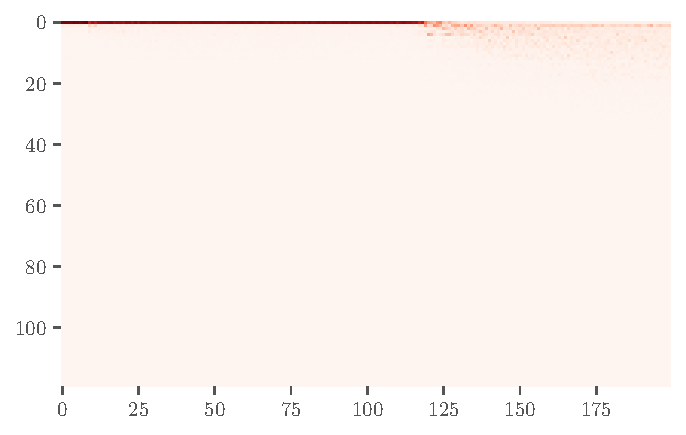
\includegraphics[width=\textwidth]{Figures/Correspondence/LeNet5_fixlr0.01/xxT_Trueest_real_corr_expand_t200_CIFAR10_Exp1_LeNet5_fixlr0.01R2_E-1_fc1.pdf}
%         \caption{$\mH$ with $\E[\vx\vx^\T]$}
%         \label{fig:Corr_xxT_True_fc}
%     \end{subfigure}%
%     \begin{subfigure}[t]{0.23\textwidth}
%         \centering
%         \captionsetup{justification=centering}
%         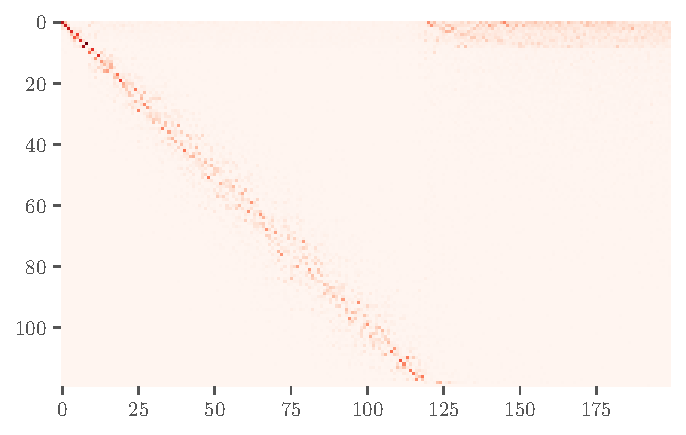
\includegraphics[width=\textwidth]{Figures/Correspondence/LeNet5_fixlr0.01/UTAU_Trueest_real_corr_expand_t200_CIFAR10_Exp1_LeNet5_fixlr0.01R2_E-1_fc1.pdf}
%         \caption{$\mH$ with $\E[\mM]$}
%         \label{fig:Corr_UTAU_True_fc}
%     \end{subfigure}%
%     \begin{subfigure}[t]{0.23\textwidth}
%         \centering
%         \captionsetup{justification=centering}
%         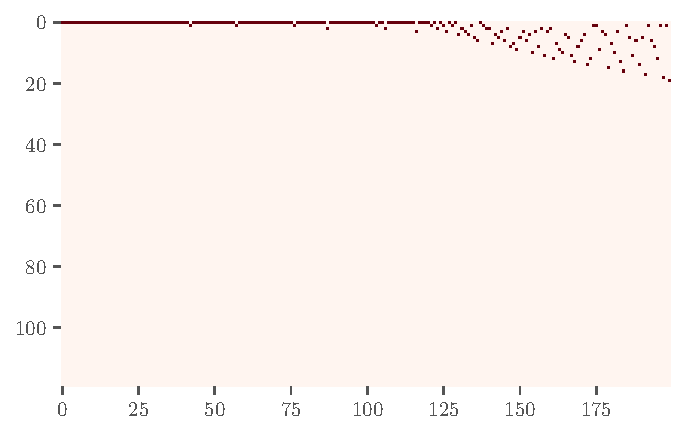
\includegraphics[width=\textwidth]{Figures/Correspondence/LeNet5_fixlr0.01/xxT_Approxest_real_corr_expand_t200_CIFAR10_Exp1_LeNet5_fixlr0.01R2_E-1_fc1.pdf}
%         \caption{$\hat{\mH}$ with $\E[\vx\vx^\T]$}
%         \label{fig:Corr_xxT_Approx_fc}
%     \end{subfigure}%
%     \begin{subfigure}[t]{0.23\textwidth}
%         \centering
%         \captionsetup{justification=centering}
%         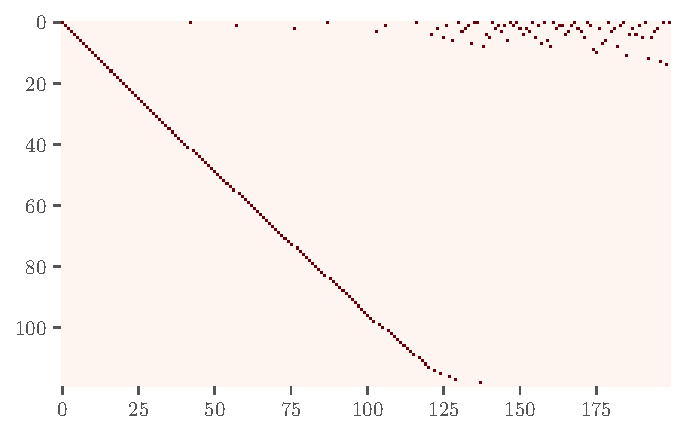
\includegraphics[width=\textwidth]{Figures/Correspondence/LeNet5_fixlr0.01/UTAU_Approxest_real_corr_expand_t200_CIFAR10_Exp1_LeNet5_fixlr0.01R2_E-1_fc1.pdf}
%         \caption{$\hat{\mH}$ with $\E[\vx\vx^\T]$}
%         \label{fig:Corr_UTAU_Approx_fc}
%     \end{subfigure}%
%     \begin{subfigure}[t]{0.032\textwidth}
%         \centering
%         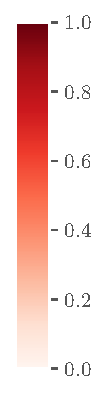
\includegraphics[width=\textwidth]{Figures/Misc/colorbar.pdf}
%     \end{subfigure}
%     }
%     %\captionsetup{justification=centering}
%     \caption{Heatmap of Eigenvector Correspondence Matrices for fc1:LeNet5, which has 120 output neurons. Here we take the top left corner of the eigenvector correspondence matrices. Similarities between (a)(c) and (b)(d) respectively verify the decoupling conjecture.}
%     \vspace{-0.1in}
%     \label{fig:Corr_fc}
% \end{figure*}

% In \figureref{fig:Corr_fc} we can see that the correspondence matrices for the true layer-wise Hessian $\mH$ approximately satisfies this property for top eigenvectors. The similarity between the correspondence patterns for the true and Kroneckor product approximated Hessian $\hat{\mH}$ also verifies the validity of the Kronecker approximation for dominate eigenspace.
% %Also note that since we are using Kronecker product to construct the approximated Hessian, the correspondence matrices of the approximated Hessian should have the ``perfect correlation''.
% From \figureref{fig:Corr_xxT_True_fc} and \figureref{fig:Corr_xxT_Approx_fc}, the top $m$ eigenvectors of the true layer-wise Hessian and the approximated Hessian are all highly correlated with $\vv_1$, the first eigenvector of $\E[\vx\vx^\T]$. From \figureref{fig:Corr_UTAU_True_fc} and \figureref{fig:Corr_UTAU_Approx_fc}, the correspondence with the $\E[\mM]$ component has a near diagonal pattern for both the true Hessian and the Kronecker approximation. Thus for small $i$ we have $\vh_i\approx \vv_1\otimes \vu_i$.
% %\rnote{Rong stopped here.}



% To understand the structure of $\E[\mM]$ itself, we consider a simplified setting where we have a random two-layer neural network with random data.
% \begin{theorem}[informal]
% For a two-layer neural network with Gaussian input, at initialization, when the network is large, the output Hessian of the first layer is approximately rank $(c-1)$ and the corresponding top eigenspace is $\gR(\mW^{(2)})\backslash\{\mW^{(2)}\cdot\textbf{1}\}$ and $\gR(\mW^{(2)})$ denotes the row space of the weight matrix $\mW^{(2)}$ of the second layer.
% \label{thm:gaussian_low_rank}
% \end{theorem}
% % To prove this theorem, we show that even after conditioning on $\mW$, the output of the network is approximately Gaussian, and is also weakly independent with the activations. These observations allows us to have a closed-form for the Hessian matrix and we leverage its form to prove the low rank structures. Note that even though the phenomenon that outputs are approximately Hessian is similar to recent works which understands wide networks as Gaussian processes \citep{lee2017deep}, the proof techniques are very different as we need to condition on $\mW$ while the Gaussian process critically relies on the fact that $\mW$ is random.

% The formal statement of this theorem and the full proof is in \sectionref{sec:appendix_low_rank}.
% The closed form calculation can be heuristically extended to the case with multiple layers, that the top eigenspace of the output Hessian of the $k$-layer would be approximately $\gR(\mS^{(k)})\setminus\{\mS^{(k)}\cdot\textbf{1}\}$,
% %$\gR\left(\mS^{(k)}\right)\setminus\{\mS^{(k)}\cdot\textbf{1}\}$, 
% %\begin{equation}
% %    \label{eqn:M-approx}
% %    \gR(\mS^{(k)})\setminus\{\mS^{(k)}\cdot\textbf{1}\}
% %\end{equation}
% where $\mS^{(k)} = \mW^{(n)}\mW^{(n-1)}\cdots\mW^{(k+1)}$ and $\gR(\mS^{(k)})$ is the row space of $\mS^{(k)}$.

% Though our result was only proven for random initialization and random data, we observe that this subspace also has high overlap with the top eigenspace of output Hessian at the minima of models trained with real datasets. The corresponding empirical results are shown in \sectionref{sec:app_outhessian_exp}. %\znote{Random Label not sufficiently discussed here: The estimation is indeed worse, which actually fits with \figureref{fig:UTAU_H_spec_RL}}
% % \begin{table}[H]
% % \vskip -0.15in
% % \caption{Overlap of $ \gR(\mS^{(k)})\setminus\{\mS^{(k)}\cdot\textbf{1}\}$ and the top $c-1$ dimension eigenspace of $\E[\mM^{(k)}]$ of different layers at minima.}
% % \vskip 0.1in
% % \begin{center}
% % \begin{small}
% % % \begin{sc}
% % \begin{tabular}{ccccccccc}
% % \toprule
% % Dataset & \multicolumn{2}{c}{MNIST} & \multicolumn{2}{c}{MNIST-R} & \multicolumn{2}{c}{CIFAR10} & \multicolumn{2}{c}{CIFAR10-R} \\
% % Network & F-$1500^3$    & LeNet5    & F-$1500^3$     & LeNet5     & F-$1500^3$     & LeNet5     & F-$1500^3$      & LeNet5     \\ \midrule
% % fc1     & 0.602         & 0.890     & 0.235          & 0.518      & 0.880          & 0.951      & 0.903           & 0.213       \\
% % fc2     & 0.967         & 0.931     & 0.801          & 0.912      & 0.943          & 0.972      & 0.931           & 0.701       \\
% % fc3     & 0.982         & 0.999     & 0.998          & 0.999      & 0.993          & 0.999      & 0.996           & 0.999     \\ \bottomrule
% % \end{tabular}
% % % \end{sc}
% % \end{small}
% % \end{center}
% % \label{tab:approx-m}
% % \vskip -0.15in
% % \end{table}
% % % \znote{This table can be compressed}
% % Note that the overlap can be low for random-label datasets which do not have a clear eigengap (as in \figureref{fig:UTAU_H_spec}). Understanding how the data could change the behavior of the Hessian is an interesting open problem. Other papers have given alternative explanations which are not directly comparable to ours, however ours is the only one that gives a closed-form formula for top eigenspace. In \sectionref{sec:appendix_M_struct} we will discuss the other explanations in more details.

% %We investigate why outliers occur in \sectionref{sec:appendix_M_struct} and explained the case at initialization.
% %Other paper has different explanations. For example,
% %\citet{papyan2019measurements} provides explanation for the low rank structure of hessian at minima using class clustering. However, in the setting of \cref{thm:gaussian_low_rank} such a clustering cannot happen because labels are also random. Our results are therefore incomparable. We discuss this in more detail in \sectionref{sec:appendix_M_struct}. \znote{The papyan paper explains the outliers at the minima using class clustering, Thm 4.1 was on initialization.}
% %\ynote{Should we mention we try to explain the outliers in the Appendix? Actually only the outlier for initialization is explained. We can say "We investigate the relation between structure of E[M] and outliers shown in Appendix" or "We explain the outliers at initialization in the Appendix"}
% %While previous work \citet{papyan2019measurements} provided some explanations for the gap using a clustering effect, such clustering does not happen in all of our experiments (and especially weak when the network is trained with random labels). 

% %\citet{papyan2019measurements} provides explanation for the gap in eigenspectrum using class clustering. Although we reproduced their results on their networks, there is no clear class clustering for both $\E[M]$ and layer-wise Hessian at the Minimum for networks we experiment on. The reason is unclear but we conjecture that class clustering is only significant for very large networks.

% %The outliers at initialization, however, are easier to explain. Similar to what \citet{papyan2019measurements} suggested for full Hessian, we observe logit clustering in $\E[\mM]$'s. Since there are $C$ logits, we would expect there are $C$ outliers. The results are shown in Appendix.

\section{Hessian Structure for Infinite Width Two-Layer ReLU Neural Network}
\label{sec:theoretical}
% In this section, we provide the proof sketch of the decoupling conjecture for the top $c-1$ eigenspace of the layer-wise parameter Hessian of a simplified setting. In particular, we consider an infinite width neural network over random data at initialization.

In this section, %we analyze the top eigenspace of the Hessian for a special network: 
we show that for a simple setting of 2-layer networks, % 2-layer infinite width neural network over random data at initialization, 
the layer-wise parameter Hessian has $c-1$ large eigenvalues and its top $c-1$ eigenspace is close to the top $c-1$ eigenspace of the Kronecker product approximation.
%\znote{not sure about the wording here} \ynote{changed wording}

\paragraph{Problem Setting and Notations}
\label{sec:theory:setting}
%In this section we will generally follow the notation defined in \sectionref{sec:prelim}. Moreover, 
Let bold non-italic letters such as $\rvv, \rmM$ denote random vectors (lowercase) and matrices (uppercase).
Consider a two layer fully connected ReLU activated neural network with input dimension $d$, hidden layer dimension $n$ and output dimension $c$. In particular, let $d=n^{1+\alpha}$ for some constant $\alpha>0$. Let the network has positive input from a rectified Gaussian $\rvx\sim \rectNormal(0, \mI_d)$ where every entry is identically distributed as $\max\{\hat{\rvx},0\}$ for $\hat{\rvx}\sim \mathcal{N}(0,1)$. %which, for a single entry, has density $f_\rectNormal(x) =\frac12\delta(x)+\frac{1}{\sqrt{2\pi}}\exp(-\frac{x^2}{2})\ind\sbr{x> 0}$ where $\delta(x)$ is the Dirac delta function. 
Let $\mW^{(1)}\in\R^{n\times d}$ and $\mW^{(2)}\in\R^{c\times n}$ be the weight matrices. In this problem we consider a random Gaussian initialization that $\mW^{(1)}\sim \cN(0,\frac1d\mI_{dn})$ and $\mW^{(2)}\sim \cN(0,\frac1n\mI_{nc})$. Both weight matrices has expected row norm of 1. Let the loss objective be cross entropy $\ell$. Training labels are irrelevant as they are independent from the Hessian at initialization. %We do not need to specify the training labels as they are independent from the Hessian at initialization.

Denote the output of the first and second layer as $\rvy$ and $\rvz$ respectively. We have $\rvy = \sigma(\mW^{(1)}\rvx)$ and $\rvz = \mW^{(2)}\rvy.$ Here $\sigma$ is the element-wise ReLU function.
Let $\rmD\triangleq\diag(\ind\sbr{\rvy\geq 0})\in\R^{n\times n}$ denote the 0/1 diagonal matrix representing the activation of $\sigma$ that $\rvy=\rmD\mW^{(1)}\rvx$.
Let $\rvp=\mbox{softmax}(\rvz)$ and let $\rmA\triangleq\diag(\rvp)-\rvp\rvp^\T$. Note $\rmA$ is rank $c-1$ with the null space of the all one vector.  We give full details about our settings in \sectionref{sec:proof-prelim}.
By simple matrix calculus (see \sectionref{sec:appendix_derivation}), the output Hessian of $\mM^{(1)}$ and the full layer-wise Hessian has closed-form
\begin{equation}
    \mM^{(1)} = \exop{\rvx\sim \rectNormal(0, \mI_d)}{\rmD\mW^{(2)\T}\rmA\mW^{(2)}\rmD}, \mH^{(1)} = \exop{\rvx\sim \rectNormal(0, \mI_d)}{\rmD\mW^{(2)\T}\rmA\mW^{(2)}\rmD\otimes \rvx\rvx^\T}.
\end{equation}
Following the decoupling conjecture, the Kronecker approximation of the layer-wise Hessian is \begin{equation}
    \hat\mH^{(1)} \triangleq \exop{\rvx\sim \rectNormal(0, \mI_d)}{\rmD\mW^{(2)\T}\rmA\mW^{(2)}\rmD}\otimes \exop{\rvx\sim \rectNormal(0, \mI_d)}{\rvx\rvx^\T}.
\end{equation}
Since we are always taking the expectation over the input $\rvx$, we will neglect the subscript and use $\E$ for expectation. Now we are ready to state our main theorem.

\begin{theorem}
\label{thm:main-full}
For an infinite width two-layer ReLU activated neural network with Gaussian initialization as defined above, let $V_1$ and $V_2$ be the top $c-1$ eigenspaces of $\mH^{(1)}$ and $\hat\mH^{(1)}$ respectively, for all $\eps>0$, 
$
    \lim_{n\to\infty}\mathop{\Pr}_{\mW^{(1)}\sim\gN(0,\frac{1}{d}\mI_{nd}), \mW^{(2)}\sim\gN(0,\frac{1}{n}\mI_{cn})}\left[\Overlap\left(V_1,V_2\right)>1-\eps\right] = 1.
$
Moreover $\mH^{(1)}$ has $c-1$ large eigenvalues that, \begin{equation}
    \lim_{n\to\infty}\mathop{\Pr}_{\mW^{(1)}\sim\gN(0,\frac{1}{d}\mI_{nd}), \mW^{(2)}\sim\gN(0,\frac{1}{n}\mI_{cn})}\left[\left(\left.\frac{\lambda_c(\mH^{(1)})}{\lambda_{c-1}(\mH^{(1)})}\right|_{\mW^{(1)}, \mW^{(2)}}\right) < \eps\right] = 1.
\end{equation}
\end{theorem}

Instead of directly working on the layer-wise Hessian, we first show a similar theorem for the output Hessian $\mM^{(1)}$. We will then show that the proof technique of the following theorem can be easily generalized to prove our main theorem.

\begin{theorem}
\label{thm:main-out}
For the same network as in \theoremref{thm:main-full}, let $\mM^*\triangleq \ex{\rmD'\mW^{(2)\T}\rmA\mW^{(2)}\rmD'}$ where $\rmD'$ is an independent copy of $\rmD$ and is independent of $\rmA$. Let $S_1$ and $S_2$ be the top $c-1$ eigenspaces of $\mM^{(1)}$ and $\mM^*$ respectively, $S_2$ is approximately $\gR\{\mW_i\}_{i=1}^c\backslash\{\textbf{1}^\T\mW\}$ where $\gR$ is the row span, and for all $\eps>0$,
$\lim_{n\to\infty}\mathop{\Pr}_{\mW^{(1)}\sim\gN(0,\frac{1}{d}\mI_{nd}), \mW^{(2)}\sim\gN(0,\frac{1}{n}\mI_{cn})}\left[\Overlap\left(S_1,S_2\right)>1-\eps\right] = 1.$
Moreover, $\mM$ has $c-1$ large eigenvalues that \begin{equation}
    \lim_{n\to\infty}\mathop{\Pr}_{\mW^{(1)}\sim\gN(0,\frac{1}{d}\mI_{nd}), \mW^{(2)}\sim\gN(0,\frac{1}{n}\mI_{cn})}\left[\left(\left.\frac{\lambda_c(\mM^{(1)})}{\lambda_{c-1}(\mM^{(1)})}\right|_{\mW^{(1)}, \mW^{(2)}}\right) < \eps\right] = 1.
\end{equation}
\end{theorem}

\textbf{Remark.}
The closed form approximating of $S_1$ in \cref{thm:main-out} can be heuristically extended to the case with multiple layers, that the top eigenspace of the output Hessian of the $k$-layer would be approximately $\gR(\mS^{(k)})\setminus\{\textbf{1}^\T\mS^{(k)}\}$
where $\mS^{(k)} = \mW^{(n)}\mW^{(n-1)}\cdots\mW^{(k+1)}$ and $\gR(\mS^{(k)})$ is the row space of $\mS^{(k)}$.
Though our result was only proven for random initialization and random data, we observe that this subspace also has high overlap with the top eigenspace of output Hessian at the minima of models trained with real datasets. The corresponding empirical results are shown in \cref{sec:app_outhessian_exp}. 

\paragraph{Proof Sketch for \theoremref{thm:main-out}}
For simplicity of notations, in this section we will use $\mW$ to denote $\mW^{(2)}$ and $\mM$ to denote $\mM^{(1)}$ unless specified otherwise.
Our proof of \theoremref{thm:main-out} mainly consists of three parts. First we analyze the structure of $\mM^*$ and show that it is approximately rank $c-1$. Then we show that $\mM^*$ and $\mM$ are roughly equivalent via an approximate independence between $\rmD$ and $\rmA$. Finally, by projecting both $\mM$ and $\mM^*$ onto a $c\times c$ matrix using $\mW$, we can apply the approximate independence and prove that the top $c-1$ eigenspace of $\mM^*$ is approximately that of $\mM$, which concludes the proof.

\paragraph{(1) Structure of $\mM^*$} When $n\to\infty$, the output of the second layer $\rvy$ converges to a multivariate Gaussian (\lemmaref{lemma:y-gaussian}), hence we can consider each diagonal entry of $\rmD$ as a $p=\frac12$ Bernoulli random variable. Since we assumed that $\rmD'$ and $\rmA$ are independent, by some simple calculation,
\begin{equation}
    \mM^*=\frac14\left(\mW^\T\E[\rmA]\mW+\text{diag}(\mW^\T\E[\rmA]\mW)\right).
\end{equation}
Here $\E[\rmA]$ is rank $c-1$ with the $(c-1)$-th eigenvalue bounded below from 0 (\lemmaref{lemma:A-rank-c-1}).
Since the two terms in the sum has the same trace while $\mW^\T\E[\rmA]\mW$ is rank $c-1$ compared to rank $n$ of $\diag(\mW^\T\E[\rmA]\mW)$, we can show that the top eigenspace is dominated by the eigenspace of $\mW^\T\E[\rmA]\mW$, which is approximately $\gR\{\mW_i\}_{i=1}^c\backslash\{\textbf{1}^\T\mW\}$. 

\paragraph{(2) Approximate Independence Between $\rmA$ and $\rmD$} Intuitively, if $\rmD$ and $\rmA$ are independent, then $\mM = \mM^*$. However, this is clearly not true - if the activations align with a row of $\mW$ then the corresponding output is going to be large, which changes $\rmA$ significantly. To address this problem, we observe that the formula for $\mM$ is only of degree 2 in $\rmD$, so one can focus on conditioning on two of the activations \--- a negligible fraction in the limit. More precisely, if one expand out the expression of each element squared in $\mM$, it is an homogeneous polynomial of the form
$p(\rmA,\rmD,\bar\rmA,\bar\rmD) = \sum_{i,j,k,l=1}^c\sum_{p,q=1}^n c_{ijklpq}\rmA_{ij}\bar\rmA_{kl}\rmD_{pp}\bar\rmD_{qq},
$
where $(\bar\rmA,\bar\rmD)$ are independent copies of $(\rmA, \rmD)$. The same element squared in $\mM^*$ is just going to be $p(\rmA,\rmD',\bar\rmA,\bar\rmD')$.
By nice properties of the Gaussian initialized weight matrix, we show that as $n\to\infty$, $\rmA$ is invariant when conditioning on two entries of $\rmD$ (\lemmaref{lemma:z-invariant}). Therefore, in the limit we have $\lim_{n\to\infty}\ex{p(\rmA, \rmD, \bar\rmA, \bar\rmD)} = \ex{p(\rmA, \rmD', \bar\rmA, \bar\rmD')}$ (detailed proof in Appendix). 
%Hence by the portmanteau theorem we have the following key lemma:
%\begin{lemma}
%\label{lemma:polynomial-maintext} (informal)
%Let $p(\rmA,\rmD,\bar\rmA,\bar\rmD)$ be a homogeneous polynomial as defined above with an upper bounded $\ell_1$ norm of the coefficients, then
%\begin{equation}
%    \lim_{n\to\infty}\ex{p(\rmA, \rmD, \bar\rmA, \bar\rmD)} = \ex{p(\rmA, \rmD', \bar\rmA, \bar\rmD')}.
%\end{equation}
%\end{lemma}

\paragraph{(3) Equivalence between $\mM^*$ and $\mM$} Since the size of $\mM$ also goes to infinity as we take the limit on $n$, it is technically difficult to directly compare their eigenspaces. In this case we utilize the fact that $\mW$ has approximately orthogonal rows, and project $\mM$ onto $\mW\mM\mW^\T$. In particular, by expanding out the Frobenious norms as polynomials and bounding the $\ell_1$ norm of the coefficients, using \lemmaref{lemma:z-invariant} we are able to show that $\fns{\mM}\approx\fns{\mW\mM\mW^\T}\approx \fns{\mW\mM^*\mW^\T}\approx \fns{\mM^*}$ (\lemmaref{lemma:M-proj-preserve-f-norm}- \lemmaref{lemma:F-norm-equal}).
This result tells us that the projection does not lose information, and hence indirectly gives us the dominating eigenspace of $\mM$. This concludes our proof for \theoremref{thm:main-out}

\paragraph{Proving \theoremref{thm:main-full} and Beyond}
To prove Theorem~\ref{thm:main-full}, we use a very similar strategy. We consider a re-scaled Hessian $\tmH\triangleq\frac1d\mH$ and show that in the independent setting $\tmH^* = \frac1d\E[\rmD'\mW\rmA\mW\rmD'\otimes \rvx''\rvx''^\T] = \mM^*\otimes\frac1d \E[\rvx''\rvx''^\T].$ We then generalize the conditioning technique to involve conditioning on two entries of $x$. 
\iffalse For simplicity of notations, we will use $\mH$ to denote $\mH^{(1)}$. Since the norm of $\mH$ goes to infinity as $n\to\infty$, we consider a re-scaled Hessian $\tmH\triangleq\frac1d\mH$. Similar to the proof for the output Hessian, we consider $\tmH^*\triangleq\frac1d\ex{\rmD'\mW\rmA\mW\rmD'\otimes \rvx''\rvx''^\T}$ that $(\rmD', \rvx'')$ are independent copies of $(\rmD, \rvx)$. Note that by the independence assumption, $\tmH^* = \frac1d\E[\rmD'\mW\rmA\mW\rmD'\otimes \rvx''\rvx''^\T] = \mM^*\otimes\frac1d \E[\rvx''\rvx''^\T].$
Since $\rvx$ is a multivariate rectified Gaussian, its mean dominates its variance for large $d$. Hence $\frac1d \E[\rvx''\rvx''^\T]$ is approximately rank-1 with the first eigenvector as $\frac{1}{\sqrt{d}}\1_d$. Combining with the result from \theoremref{thm:main-out}, the top eigenspace of $\tmH$ is just $\gR\{\frac{1}{\sqrt{d}}\mW_i\otimes\1_d^\T\}_{i=1}^c\backslash\{\frac{1}{\sqrt{d}}\mW\otimes\1_d^\T\cdot\textbf{1}\}$.
We may generalize \lemmaref{lemma:polynomial-maintext} so that we can condition on two extra entries of $\rvx$ (\corollaryref{cor:polynomial}), and finally establish the equivalence between $\tmH$ and $\tmH^*$ by projection using $\mW\otimes\1_d$ (\lemmaref{lemma:H-proj-preserve-f-norm}- \lemmaref{lemma:F-norm-equal-H}). Following similar arguments of the output Hessian conclude the proof.

\paragraph{Remark}
Using the same proof strategy, we can generalize the theorem to the second layer-wise Hessian $\mH^{(2)} = \E[\rmA\otimes \rvy\rvy^\T]$. Moreover, since \lemmaref{lemma:polynomial-maintext} can be generalized to include activations and inputs of multiple layers, this proof technique can be generalized to deal with deeper networks.
\fi

\section{Empirical Observation and Verification}
\label{sec:empirical}
In this section, we present some empirical observations that either verifies, or are induced by the decoupling conjecture.
We conduct experiments on the CIFAR-10, CIFAR-100  \citep{Krizhevsky09learningmultiple}, and MNIST  \citep{lecun1998gradient} datasets as well as their random labeled versions, namely MNIST-R and CIFAR10-R. 
% We use PyTorch \citep{NEURIPS2019_9015} framework for all experiments.
We used different fully connected (fc) networks (a fc network with $m$ hidden layers and $n$ neurons each hidden layer is denoted as F-$n^m$), several variations of LeNet \citep{lecun1998gradient}, VGG11 \citep{simonyan2014very}, and ResNet18 \citep{kaiming2015}.
% The results shown in the main text are from variants of VGG11 and ResNet18 trained on CIFAR100, variants of LeNet5 trained on CIFAR10, and F-$200^2$ trained on MNIST.
% The eigenvalues and eigenvectors of the exact layer-wise Hessians are approximated using a modified Lanczos algorithm \citep{hessian-eigenthings} which is described in detail in \sectionref{sec:appendix_eigencomp}. 
We use ``layer:network'' to denote a layer of a particular network. For example, conv2:LeNet5 refers to the second convolutional layer in LeNet5.
More empirical results are included in \sectionref{sec:appendix_exp_res}.

\subsection{Kronecker Approximation of Layer-wise Hessian and Full Hessian}\label{subsec:approx}

% \begin{figure}[h]
% \centering
% \vspace{-1em}
% \subfigure[\small{Top eigenvalues of\\ $\mH_\cL^{(i)}$ and $\hat\mH_\cL^{(i)}$ (fc1)}]{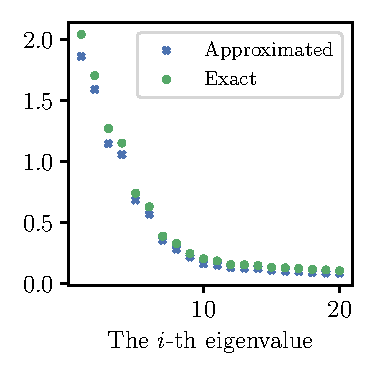
\includegraphics[width=0.24\linewidth]{Figures/ApproxQuality/FC2_fixlr/eigenval_compare_top20_MNIST_Exp1_FC2_fixlr0.01R2_E-1_narrow_fc1.pdf}}
% \subfigure[\small{Eigenspace overlap\\ of $\hat\mH^{(i)}_\cL$ and $\mH^{(i)}_\cL$}]{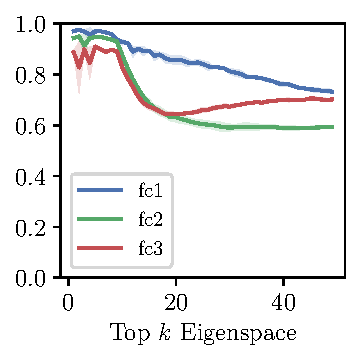
\includegraphics[width=0.24\linewidth]{Figures/ApproxQuality/FC2_fixlr/sample_kron_decomp_traceoverlap_d80_MNIST_Exp1_FC2_fixlr0.01Average_E-1_narrow.pdf}}
% \subfigure[\small{Top eigenvalues of\\ $\mH_\cL$ and $\hat\mH_\cL$ (full)}]{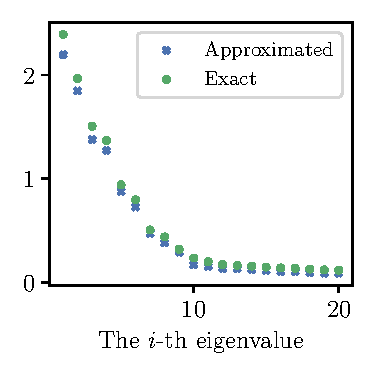
\includegraphics[width=0.24\linewidth]{Figures/ApproxQuality/FC2_fixlr/MNIST_Exp1_FC2_fixlr0.01_fulleigenval_approx.pdf}}
% \subfigure[\small{Eigenspace overlap\\ of $\hat\mH_\cL$ and $\mH_\cL$}]{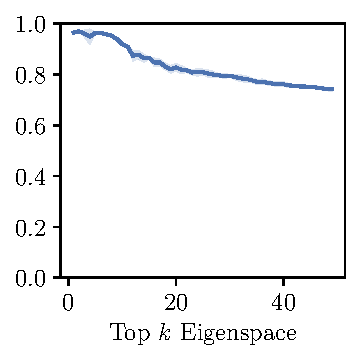
\includegraphics[width=0.24\linewidth]{Figures/ApproxQuality/FC2_fixlr/MNIST_Exp1_FC2_fixlr0.01_Average_fulleigenvec_overlap.pdf}}
% \caption{Comparison between the approximated and true layer-wise Hessian of F-$200^2$. $\mH^{(i)}_\cL$ denote the layer-wise Hessian, and $\mH_\cL$ denote the full Hessian including off-diagonal blocks. The approximated full Hessian $\hat\mH_\cL$ is defined in \sectionref{sec:appendix_full_hessian}}
% \label{fig:eigeninfo_approx}
% \vspace{-1em}
% \end{figure}

% To verify our approximation using Kronecker factorization, we compare the top eigenvalues and eigenspaces of the approximated Hessian and the true Hessian. We use the standard definition of subspace overlap (\cref{def:overlap}) to measure the similarity between top eigenspaces. %We define the dimension $k$ top eigenspace of a matrix as the subspace spanned by the eigenvectors corresponding to its $k$ largest eigenvalues. 
To verify the decoupling conjecture in practical settings, we compare the top eigenvalues and eigenspaces of the approximated Hessian and the true Hessian. We use subspace overlap (\definitionref{def:overlap}) to measure the similarity between top eigenspaces. As shown in \figureref{fig:eigeninfo_approx}, this approximation works reasonably well on the top eigenspace.

\begin{figure}[ht]
    \centering
\begin{subfigure}[b]{0.24\columnwidth}
    \captionsetup{justification=centering}
    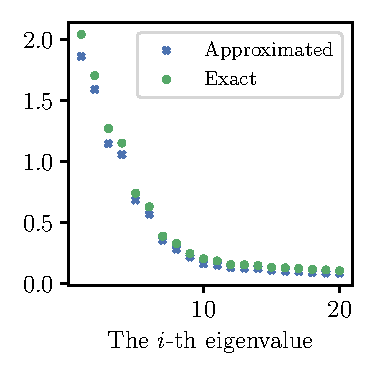
\includegraphics[width=\columnwidth]{Figures/ApproxQuality/FC2_fixlr/eigenval_compare_top20_MNIST_Exp1_FC2_fixlr0.01R2_E-1_narrow_fc1.pdf}
    \vspace{-0.2in}
    \caption{Top eigenvalues of layer-wise Hessian of fc1}
    % \caption{Eigenvalues}
    \label{fig:eigenval_approx}
\end{subfigure}%
\begin{subfigure}[b]{0.24\columnwidth}
    \captionsetup{justification=centering}
    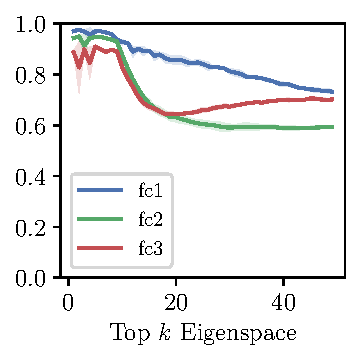
\includegraphics[width=\columnwidth]{Figures/ApproxQuality/FC2_fixlr/sample_kron_decomp_traceoverlap_d80_MNIST_Exp1_FC2_fixlr0.01Average_E-1_narrow.pdf}
    \vspace{-0.2in}
    \caption{Top eigenspace of layer-wise Hessians}
    % \caption{Eigenspace overlap}
    \label{fig:overlap_approx}
\end{subfigure}
\begin{subfigure}[b]{0.24\columnwidth}
    \captionsetup{justification=centering}
    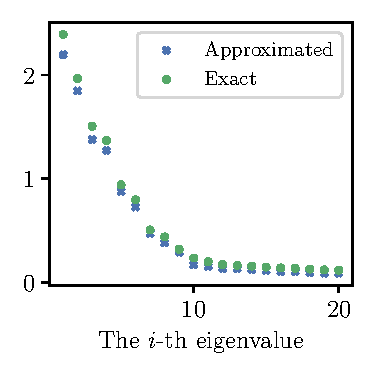
\includegraphics[width=\columnwidth]{Figures/ApproxQuality/FC2_fixlr/MNIST_Exp1_FC2_fixlr0.01_fulleigenval_approx.pdf}
    \vspace{-0.2in}
    \caption{Top eigenvalues of the full Hessian}
    % \caption{Eigenspace overlap}
    \label{fig:eigenval_approx_full}
\end{subfigure}
\begin{subfigure}[b]{0.24\columnwidth}
    \captionsetup{justification=centering}
    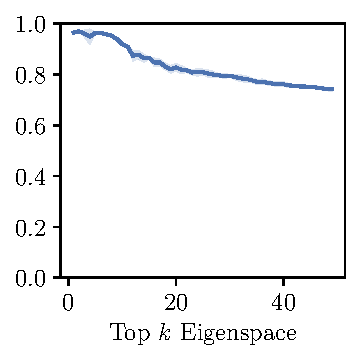
\includegraphics[width=\columnwidth]{Figures/ApproxQuality/FC2_fixlr/MNIST_Exp1_FC2_fixlr0.01_Average_fulleigenvec_overlap.pdf}
    \vspace{-0.2in}
    \caption{Top eigenspace of the full Hessian}
    % \caption{Eigenspace overlap}
    \label{fig:overlap_approx_full}
\end{subfigure}
% \vspace{-0.2in}
\caption{Comparison between the approximated and true layer-wise Hessian of F-$200^2$.}
\vspace{-4pt}
\label{fig:eigeninfo_approx}
\end{figure}
%for the top eigenvalues and eigenspaces of both layer-wise weight Hessians and the full parameter Hessian.
%In this section we leverage the Kronecker factorization to understand structures of the dominating eigenspace of layerwise Hessians.
\subsection{Low Rank Structure of \texorpdfstring{$\E[\mM]$}{EM} and \texorpdfstring{$\mH$}{H}}
\label{sec:emp_outlier}
Another way to empirically verify the decoupling conjecture is to show the similarity between the outliers in eigenspectrum of the layer-wise Hessian $\E[\mM]$ and the output Hessian $\mH_\cL$.
%We can also conjecture that the outliers also appear in $\E[\mM]$.
\figureref{fig:UTAU_H_spec} shows the similarity of eigenvalue spectrum between $\E[\mM]$ and layer-wise Hessians in different situations, which agrees with our prediction. For (a) and  (b) we are also seeing the eigengap at $c-1$, which is consistent with our analysis and previous observations \citep{sagun2017empirical,papyan2019measurements}. However, the eigengap does not appear at minimum for random labeled data with a under-parameterized network, meaning that our theory may not generalize to all settings.

\begin{figure*}[h]
\resizebox{\textwidth}{!}{%
    \centering
    \captionsetup[sub]{format=subcaptionformat}
    \begin{subfigure}[b]{0.3\textwidth}
        \centering
        \captionsetup{justification=centering}
        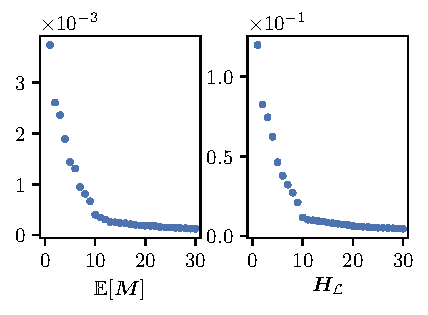
\includegraphics[width=\textwidth]{Figures/EM_vs_H/LeNet5_fixlr_0.01_init/UTAU_vs_full_sigval_d30_CIFAR10_Exp1_LeNet5_fixlr0.01R1_E0_fc1.pdf}
        \caption{fc1:LeNet5 at initialization (CIFAR10).}
        \label{fig:UTAU_H_spec_FC2}
    \end{subfigure}%
    \begin{subfigure}[b]{0.3\textwidth}
        \centering
        \captionsetup{justification=centering}
        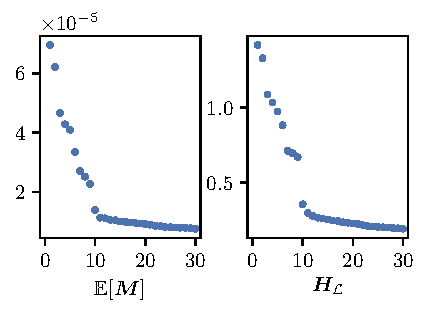
\includegraphics[width=\textwidth]{Figures/EM_vs_H/LeNet5_fixlr0.01/UTAU_vs_full_sigval_d30_CIFAR10_Exp1_LeNet5_fixlr0.01R1_E-1_fc1.pdf}
        \caption{fc1:LeNet5 at minimum\\ (CIFAR10).}
        \label{fig:UTAU_H_spec_Lenet}
    \end{subfigure}%
    \begin{subfigure}[b]{0.3\textwidth}
        \centering
        \captionsetup{justification=centering}
        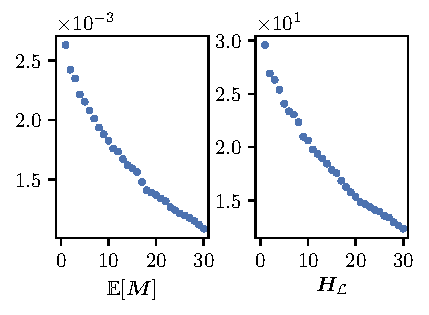
\includegraphics[width=\textwidth]{Figures/EM_vs_H/LeNet5_RL/UTAU_vs_full_sigval_d30_CIFAR10_RandomLabel_LeNet5_fixlr0.01_RLR4_E-1_fc1.pdf}
        \caption{fc1:LeNet5 at minimum\\ (CIFAR10-R).}
        \label{fig:UTAU_H_spec_RL}
    \end{subfigure}%
    }
     %\captionsetup{justification=centering}
    
    \caption{Eigenspectrum of the layer-wise output Hessian $\E[\mM]$ and the layer-wise weight Hessian $\mH_\Ls(\vw^{(p)})$. The vertical axes denote the eigenvalues. Similarity between the two eigenspectra is a direct consequence of a low rank $\E[\vx\vx^T]$ and the decoupling conjecture.}
    \label{fig:UTAU_H_spec}
    \vskip -0.05in
\end{figure*}

% \begin{figure}[h]
%     \centering
%     % \vspace{-1em}
%     \subfigure[\small{fc1:LeNet5 at init\\ (CIFAR10)}]{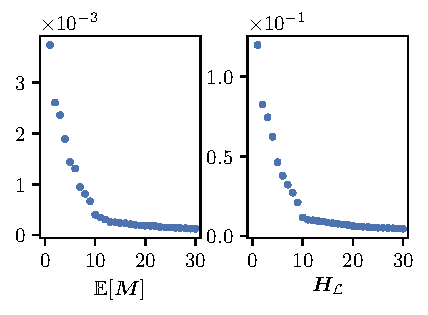
\includegraphics[width=0.25\linewidth]{Figures/EM_vs_H/LeNet5_fixlr_0.01_init/UTAU_vs_full_sigval_d30_CIFAR10_Exp1_LeNet5_fixlr0.01R1_E0_fc1.pdf}}
%     \qquad
%     \subfigure[\small{fc1:LeNet5 at min\\ (CIFAR10)}]{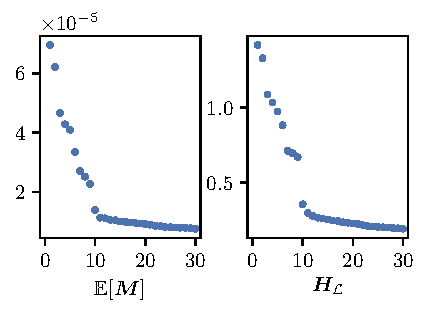
\includegraphics[width=0.25\linewidth]{Figures/EM_vs_H/LeNet5_fixlr0.01/UTAU_vs_full_sigval_d30_CIFAR10_Exp1_LeNet5_fixlr0.01R1_E-1_fc1.pdf}}
%     \qquad
%     \subfigure[\small{fc1:LeNet5 at min\\ (CIFAR10-R)}]{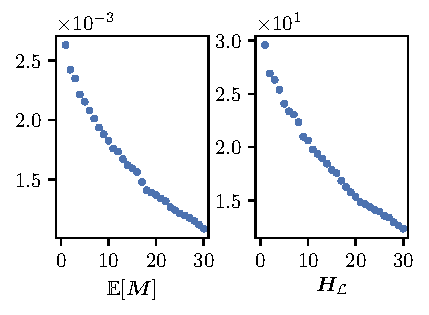
\includegraphics[width=0.25\linewidth]{Figures/EM_vs_H/LeNet5_RL/UTAU_vs_full_sigval_d30_CIFAR10_RandomLabel_LeNet5_fixlr0.01_RLR4_E-1_fc1.pdf}}
%     \caption{Eigenspectrum of the layer-wise output Hessian $\E[\mM]$ and the layer-wise weight Hessian $\mH_\Ls(\vw^{(p)})$. The vertical axes denote the eigenvalues. Similarity between the two eigenspectra is a direct consequence of a low rank $\E[\vx\vx^\T]$ and the decoupling conjecture.}
%     \label{fig:UTAU_H_spec}
%     \vspace{-2.5em}
% \end{figure}

% \subsection{Dominating Eigenvectors of Layer-wise Hessian are Low Rank}
% \label{sec:domin_eig}
% Here we verify the second prediction in \sectionref{sec:conjecture-implication}. From \figureref{fig:eigenvector-lowrank}
% for top eigenvector $\vh_i$, $\norm{\Mat(\vh_i)}$ is at least $\fn{\Mat(\vh_i)}/2$ (and often much larger), indicating the top eigenvectors of the layer-wise Hessians are very close to rank 1 after matricization.
% \begin{figure}[h]
% % \vskip -0.1in
% \centering
%     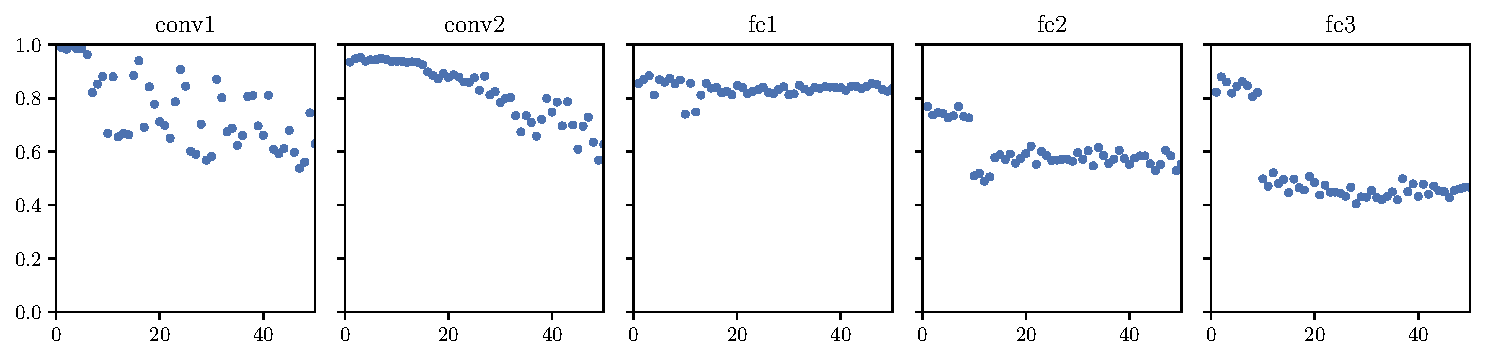
\includegraphics[width=0.75\columnwidth]{Figures/Eigenvec_Lowrank/NLeNet_base/5x1_Top_Eigenvector_rank_CIFAR10_Exp1_LeNet5_normnew_fixlr0.01R2_E-1_50.pdf}
%     %\captionsetup{justification=centering}
%     \vspace{-0.2in}
%     \caption{Ratio between top singular value and Frobenius norm of matricized dominating eigenvectors. (LeNet5 on CIFAR10). The horizontal axes denote the index $i$ of eigenvector $\vh_i$, and the vertical axes denote $\|\Mat(\vh_i)\|/\|\Mat(\vh_i)\|_F$.}
%     \label{fig:eigenvector-lowrank}
%     \vspace{-2.5em}
% \end{figure}
%\figureref{fig:eigen_lowrank} shows first singular values of $\Mat(\vh_i)$ divided by its Frobenius Norm for $i$ from 1 to 200. We can see that the top eigenvectors of the layer-wise Hessians are very close to rank 1.
% \znote{This figure does not contain much information}
% \begin{figure}[h]
% % \vskip -0.1in
% \centering
%     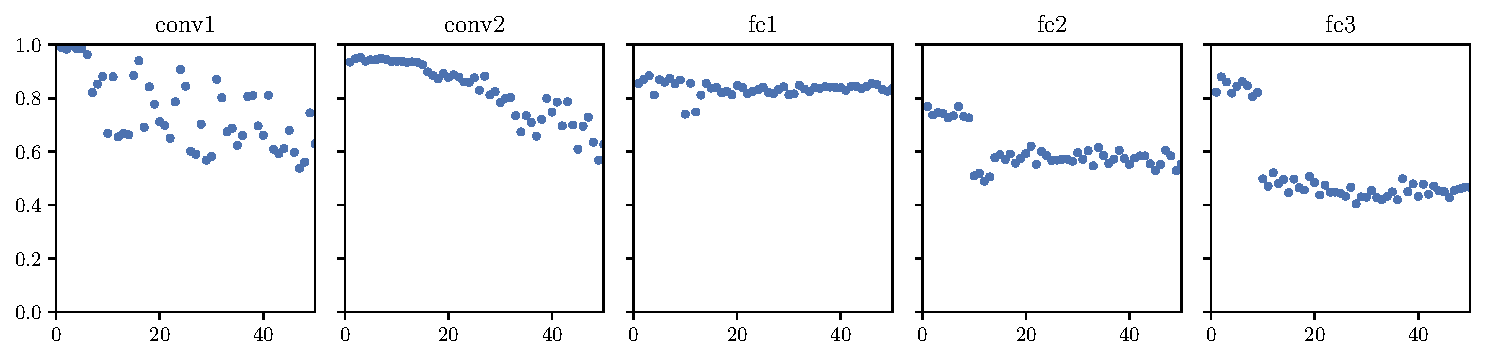
\includegraphics[width=0.75\columnwidth]{Figures/Eigenvec_Lowrank/NLeNet_base/5x1_Top_Eigenvector_rank_CIFAR10_Exp1_LeNet5_normnew_fixlr0.01R2_E-1_50.pdf}
%     %\captionsetup{justification=centering}
%     \vspace{-0.2in}
%     \caption{Ratio between top singular value and Frobenius norm of matricized dominating eigenvectors. (LeNet5 on CIFAR10). The horizontal axes denote the index $i$ of eigenvector $\vh_i$, and the vertical axes denote $\|\Mat(\vh_i)\|/\|\Mat(\vh_i)\|_F$.}
%     \label{fig:eigenvector-lowrank}
%     \vspace{-2.5em}
% \end{figure}

\subsection{Eigenspace Overlap of Different Models}
\label{sec:models}
Apart from the phenomena that are direct consequences of the decoupling conjecture, we observe another nontrivial phenomenon involving different minima.
Consider models with the same structure, trained on the same dataset, but using different random initializations, despite no obvious correlation between their parameters, we observe surpisingly high overlap between the dominating eigenspace of some of their layer-wise Hessians.
% \begin{figure}[h]
% \centering
% % \vspace{-1em}
% \subfigure[\small{conv12:ResNet18} ]{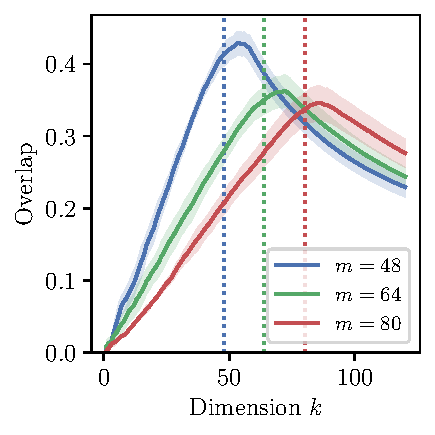
\includegraphics[width=0.25\linewidth]{Figures/SubspaceOverlap/NeurIPS/Overlap_ResNet_conv12.conv1.pdf}}
% \quad
% \subfigure[\small{conv6:VGG11} ]{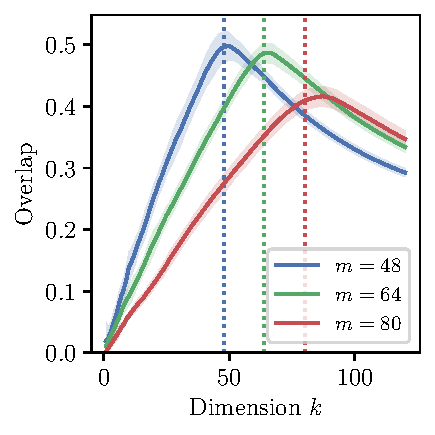
\includegraphics[width=0.25\linewidth]{Figures/SubspaceOverlap/NeurIPS/VGG11_conv6.pdf}}
% \quad
% \subfigure[\small{fc1:LeNet5} ]{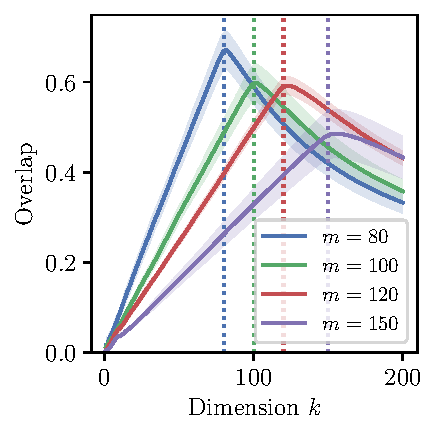
\includegraphics[width=0.25\linewidth]{Figures/SubspaceOverlap/NeurIPS/LeNetVarying.pdf}}
% \caption{Overlap between the top $k$ dominating eigenspace of different independently trained models. In each figure, we vary the number of output neuron/channels $m$. We includes 4 variants of LeNet5 trained on CIFAR10 (a), 3 variants of ResNet18 trained on CIFAR100 (b), and 3 different of VGG11 trained on CIFAR100 (c). For each structural variant, 5 models are trained from independent random initializations. We plot the average pairwise overlap between the top eigenspaces of those models' layer-wise Hessians. The overlap peaks at the output dimension $m$.}
% \label{fig:overlap}
% \vspace{-1em}
% \end{figure}


\begin{figure}[H]
    \captionsetup[sub]{format=subcaptionformat}
    \centering
    \begin{subfigure}[h]{0.32\columnwidth}
        \centering
        \captionsetup{justification=centering}
        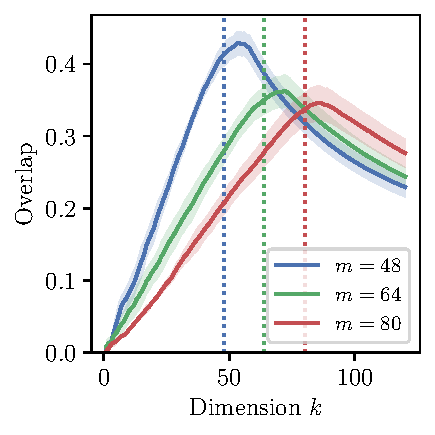
\includegraphics[width=\textwidth]{Figures/SubspaceOverlap/NeurIPS/Overlap_ResNet_conv12.conv1.pdf}
        \vspace{-0.2in}
        \caption{conv12:ResNet18 (CIFAR100) with 48/64/80 output channels}

        \label{fig:Overlap_resnet_conv1}
    \end{subfigure}
    \begin{subfigure}[h]{0.32\columnwidth}
        \centering
        \captionsetup{justification=centering}
        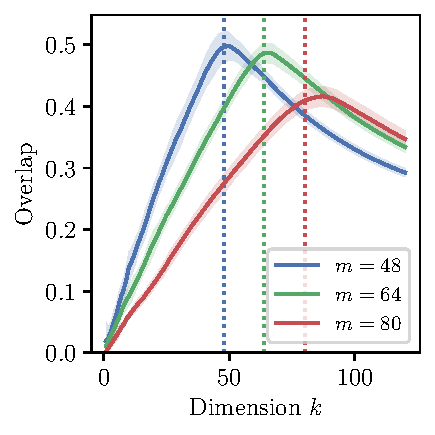
\includegraphics[width=\textwidth]{Figures/SubspaceOverlap/NeurIPS/VGG11_conv6.pdf}
        \vspace{-0.2in}
        \caption{conv6:VGG11 (CIFAR100) with 48/64/80 output channels}

        \label{fig:Overlap_resnet_conv2}
    \end{subfigure}
    \begin{subfigure}[h]{0.32\columnwidth}
        \centering
        \captionsetup{justification=centering}
        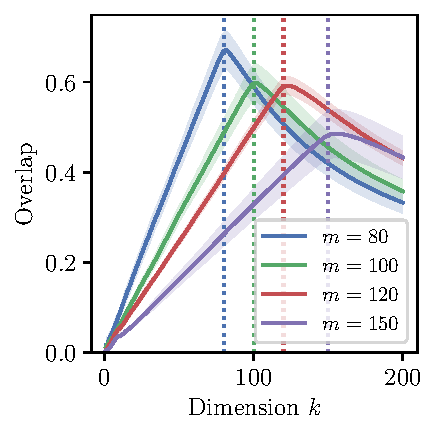
\includegraphics[width=\textwidth]{Figures/SubspaceOverlap/NeurIPS/LeNetVarying.pdf}
        \vspace{-0.2in}
        \caption{fc1:LeNet5 (CIFAR10) with 80/100/120/150 output neurons}

        \label{fig:Overlap_fc1}
    \end{subfigure}
    %\captionsetup{justification=centering}

    \caption{Overlap between the top $k$ dominating eigenspace of different independently trained models. The overlap peaks at the output dimension $m$. The eigenspace overlap is defined in \cref{def:overlap}.}
    \label{fig:overlap}
    \vskip -0.1in
\end{figure}

It turns out that the nontrivial overlap is also a consequence of the decoupling conjecture, which arises when the output Hessian and autocorrelation are related in the following way: When the small eigenvalues of $\E[\mM]\in\R^{m\times m}$ approaches 0 slower than the small eigenvalues of $\E[\vx\vx^\T]$, the top $m$ eigenspace will then be approximately spanned by $\mI_m\otimes \E[\vx]^\T$ by the decoupling conjecture.
Now suppose we have two different models with $\hE[\vx]_1$ and $\hE[\vx]_2$ respectively. Their top-$m$ eigenspaces are approximately $\mI_m \otimes \hE[\vx]_1$ and $\mI_m \otimes \hE[\vx]_2$. Thus the overlap at dimension $m$ is approximately $(\hE[\vx]_1^\T \hE[\vx]_2)^2$, which is large since $\hE[\vx]_1$ and $\hE[\vx]_2$ are the same for the input layer and all non-negative for other layers.
While this particular relation between $\E[\mM]$ and $\E[\vx\vx^\T]$ are true in many shallow networks and in later layers of deeper networks, they are not satisfied for earlier layers of deeper networks.  In \sectionref{sec:appendix_model_overlap} we explain how one can still understand the overlap using correspondence matrices when the above simplified argument does not hold. %why the overlap before rank-$m$ grows linearly. We also make a more general explanation and account for some cases where this argument does not hold. 

%Note that fc3 does not have the linear growth since neurons cannot be permuted in the last layer. \ynote{In addition, for the first layer, models with the same dataset would have the same $\hE[\vx]$, and that would lead to an overlap close to 1 at dimension $n$. Omit since we did not show the first layer}

%Then, consider the $(m+1)$th eigenvector of the first model. Since top $n$ eigenvectors span the full space $\Krsp(\hE[\vx]_1)$, it will be orthogonal to this space. It will also have low overlap with $\Krsp(\hE[\vx]_2)$ since $(\hE[\vx]_1 \cdot \hE[\vx]_2)$ is large. This explains the immediate drop in eigenspace overlap at dimension $m+1$. \ynote{May not be necessary}

% \subsection{Batch Normalization and Zero-mean Input}
% \snote{The approximation worsen, but is still relevant. Reason of low overlap: low correlation between $x$ in different layers, random permutation of neurons in FC layers.}
% According to our explanation, the good approximation and high overlap of top eigenspace both depend on the low rank structure of $\E[\vx\vx^T]$. Also, the low rank structure is caused by the fact that $\E[\vx]\E[\vx]^T$ dominates $\mSigma_\vx$ in most cases. Therefore, it's natural to conjecture that models trained using Batch Normalization (BN) \citep{ioffe2015batch} will change these phenomena as $\E[\vx]$ will be zero and $\E[\vx\vx^T] = \mSigma_\vx$ for those models. Indeed, as shown in \citet{ghorbani2019investigation}, BN suppresses the outliers in the Hessian eigenspectrum and \citet{papyan2020traces} provided an explanation.

% We experiment on our networks with BN. The results are shown in \sectionref{sec:appendix_batchnorm}. We found that $\E[\vx\vx^T]$ is no longer close to rank 1 for models trained with BN. However, $\E[\vx\vx^T]$ still have a few large eigenvalues. % and is not similar to a random matrix.
% In this case, all the previous structures ($c$ outliers, high eigenspace overlap, low rank eigenvectors) become weaker. The decoupling conjecture itself also becomes less accurate. However, the approximation still gives meaningful information. %our approximation in \sectionref{sec:approx_top_eig} is not accurate. Thus, the overlap of top $k$ eigenspace between different models can no longer be approximated as in \cref{eqn:model_overlap}. As expected, models with BN give a much lower eigenspace overlap at dimension smaller than $n$ and there is no obvious peak.

%The approximation of Hessian eigenvalues using Kronecker factorization is also not so accurate in models using BN, agreeing with our conjecture. However, the approximation still gives meaningful information and the top eigenspace overlap between true and approximated hessian is still (). It is lower than the case without BN but much larger than the expected value for 2 random subspaces.

% \paragraph{Remark} \znote{Batchnorm}

\section{Tighter PAC-Bayes Bound with Hessian Information}
\label{sec:appendix_pac}
Given a model parameterized with $\theta$ and an input-label pair $(\vx,\vy)\in\R^d\times \R^c$, the classification error of $\theta$ over the input sample $\vx$ is $\breve{l}(\theta, \vx) := \1[\arg\max f_\theta(\vx) = \arg\max\vy].$ With the underlying data distribution $D$ and training set $S$ i.i.d. sampled from $D$, we define
\begin{equation}
e(\theta):=\E_{(\vx, \vy)\sim D}[\breve{l}(\theta,\vx)],\qquad \hat{e}(\theta):=\frac{1}{N}\sum_{i=1}^N[\breve{l}(\theta,\vx_i)]
\end{equation}
as the expected and empirical classification error of $\theta$, respectively.
We define the measurable hypothesis space of parameters $\gH:= \R^P$.
%\znote{measurability is STATEd for KL to be generally well-defined, do we need to define $P$ and $Q$ as probability measure as well?}
For any probabilistic measure $P$ in $\gH$, let $e(P) = \E_{\theta\sim P}e(\theta)$, $\hat{e}(P) = \E_{\theta\sim P}\hat{e}(\theta)$, and $\breve{e}(P) = \E_{\theta\sim P}\mathcal{L}(\theta)$. Here $\breve{e}(P)$ serves as a differentiable convex surrogate of $\hat{e}(P).$

\begin{theorem}[Pac-Bayes Bound]
\citep{mcallester1999some}\citep{langford2001bounds}
For any prior distribution $P$ in $\gH$ that is chosen independently from the training set $S$, and any posterior distribution $Q$ in $\gH$ whose choice may inference $S$, with probability $1-\delta$,
\begin{equation}
    \label{eqn:appendix_pac_bayes_inf}
    \KL\left(\hat{e}(Q)\Vert e(Q)\right)\leq \frac{\KL(Q\Vert P) + \log\frac{|S|}{\delta}}{|S|-1}.
\end{equation}
\end{theorem}
Fix some constant $b, c \geq 0$ and $\theta_0\in\gH$ as a random initialization, \citet{dziugaite2017computing} shows that when setting $Q = \gN(\vw, \diag(\vs))$, $P = \gN(\theta_0, \lambda\mI_P)$, where $\vw, \vs\in\gH$ and $\lambda = c\exp{(-j/ b)}$ for some $j\in\mathbb{N}$, and solve the optimization problem
\begin{equation}
    \min_{\vw,\vs,\lambda}\breve{e}(Q) + \sqrt{\frac{\KL(Q\Vert P) + \log\frac{|S|}{\delta}}{2(|S|-1)},}
\end{equation} with initialization $\vw = \theta$, $\vs = \theta^2$,
one can achieved a nonvacous PAC-Bayes bound by \equationref{eqn:appendix_pac_bayes_inf}.

In order to avoid discrete optimization for $j\in \N$, \citet{dziugaite2017computing} uses the $\BRE$ term to replace the bound in \tableref{eqn:appendix_pac_bayes_inf}. The $\BRE$ term is defined as
\begin{equation}
    \BRE(\vw,\vs,\lambda; \delta) = \frac{\KL(P\Vert Q)+2\log(b\log \frac{c}{\lambda})+\log \frac{\pi^2 |S|}{6\delta}} {|S|-1},
\end{equation}
where $Q = \gN(\vw, \diag(\vs))$, $P = \gN(\theta_0, \lambda\mI_P)$.
The optimization goal actually used in the implementation is thus
\begin{equation}
    \min_{\vw \in \R^P,\vs\in \R^P_+,\lambda\in (0,c)}\breve{e}(Q) + \sqrt{\frac{1}{2}\BRE(\vw,\vs,\lambda; \delta)}.
\end{equation}

\algorithmref{alg:pac} shows the algorithm for \emph{Iterative Hessian} (\textsc{Iter}) PAC-Bayes Optimization. If we set $\eta = T$, the algorithm will be come \emph{Approximate Hessian} (\textsc{Appr}) PAC-Bayes Optimization. It is based on Algorithm 1 in \citet{dziugaite2017computing}. The initialization of $\vw$ is different from \citet{dziugaite2017computing} because we believe what they wrote, $\abso(\vw)$ is a typo and $\log[\abso(\vw)]$ is what they actually means. It is more reasonable to initialize the variance $\vs$ as $\vw^2$ instead of $\exp[2\abso(\vw)]$.

\begin{algorithm}[ht]
\caption{PAC-Bayes bound optimization using layer-wise Hessian eigenbasis}
\textbf{Input:}\\
\algind$\vw_0\in\R^P$\Comment{Network parameters (Initialization)}\\
\algind$\vw\in \R^P$\Comment{Network parameters (SGD solution)}\\
\algind$S$ \Comment{Training examples}\\
\algind$\delta \in (0,1)$ \Comment{Confidence parameter}\\
\algind$b \in \mathbb{N}, c \in (0,1)$ \Comment{Precision and bound for $\lambda$}\\
\algind$\tau\in(0,1), T \in\mathbb{N}$ \Comment{Learning rate; No. of iterations}\\
\algind$\eta \in \mathbb{N}$ \Comment{Epoch interval for Hessian calculation}\\
\textbf{Output}\\
\algind$\vw$\Comment{Optimized network parameters}\\
\algind$\vs$\Comment{Optimized posterior variances in Hessian eigenbasis}\\
\algind$\lambda$\Comment{Optimized prior variancce}
\begin{algorithmic}[1]
\Procedure{Iterative-Hessian-PAC-Bayes}{}
    \State $\vvarsigma \gets \log[\abso(\vw)]$\Comment{where $\vs(\vvarsigma)= \exp(2\vvarsigma)$}
    \State $\varrho \gets -3$\Comment{where $\lambda(\varrho) = \exp(2\varrho)$}
    \State $R(\vw, \vs, \lambda) = \sqrt{\frac{1}{2}\BRE(\vw,\vs,\lambda; \delta)}$
    \Comment{BRE term}
    \State $B(\vw,\vs,\lambda,\vw') = \Ls(\vw')+R(\vw,\vs,\lambda)$\Comment{Optimization goal}
    \For{$t = 0 \to T-1$}\Comment{Run SGD for T iterations}
        \If{$t\mod \eta == 0$}
            \State $\textsc{HessianCalc}(w)$
        \EndIf
        \State \text{Sample} $\vxi \sim \N(0,1)^P$ 
        \State $\vw'(\vw,\vvarsigma)= \vw +\textsc{ToStandard}\left(\vxi \odot \exp(\vvarsigma)\right)$ \Comment{Generate noisy parameter for SNN}
        \State $\vw \gets \vw- \tau\left[\nabla_\vw R(\vw, \vs, \lambda)+\nabla_{\vw'}\Ls(\vw')\right]$
        \State $\vvarsigma \gets \vvarsigma - \tau\left[\nabla_\vvarsigma R(\vw, \vs(\vvarsigma), \lambda)+\textsc{ToHessian}\left(\nabla_{\vw'}\Ls(\vw')\right)\odot \vxi \odot \exp(\vvarsigma)\right]$
        \State $\varrho \gets \varrho - \tau\nabla_{\varrho}R(\vw,\vs,\lambda(\varrho))$ \Comment{Gradient descent}
    \EndFor
    \State \Return $w, s(\vvarsigma), \lambda(\varrho)$
\EndProcedure
\end{algorithmic}
\label{alg:pac}
\end{algorithm}

% \begin{algorithm2e}[ht]
% \caption{PAC-Bayes bound optimization using layer-wise Hessian eigenbasis}
% \SetKwInOut{KwInput}{Input}
% \SetKwInOut{KwOutput}{Output}
% \KwInput{
% $\vw_0\in\R^P$\tcp{Network parameters (Initialization)}
% $\vw\in \R^P$\tcp{Network parameters (SGD solution)}
% $S$ \tcp{Training examples}
% $\delta \in (0,1)$ \tcp{Confidence parameter}
% $b \in \mathbb{N}, c \in (0,1)$ \tcp{Precision and bound for $\lambda$}
% $\tau\in(0,1), T \in\mathbb{N}$ \tcp{Learning rate; No. of iterations}
% $\eta \in \mathbb{N}$ \tcp{Epoch interval for Hessian calculation}}
% \KwOutput{
% $\vw\in \R^P$\tcp{Optimized network parameters}
% $\vs\in \R^P$\tcp{Optimized posterior variances in Hessian eigenbasis}
% $\lambda \in \R_+$\tcp{Optimized prior variancce}}
% \Begin{
%     $\vvarsigma \gets \log[\abso(\vw)]$\tcp{where $\vs(\vvarsigma)= \exp(2\vvarsigma)$}
%     $\varrho \gets -3$\tcp{where $\lambda(\varrho) = \exp(2\varrho)$}
%     $R(\vw, \vs, \lambda) = \sqrt{\frac{1}{2}\BRE(\vw,\vs,\lambda; \delta)}$
%     \tcp{BRE term}
%     $B(\vw,\vs,\lambda,\vw') = \Ls(\vw')+R(\vw,\vs,\lambda)$\tcp{Optimization goal}
%     \For(\tcp*[h]{Run SGD for T iterations}){$t = 0 \to T-1$} {
%         \If{$t\mod \eta == 0$} {
%             $\textsc{HessianCalc}(w)$
%         }
%     Sample $\vxi \sim \N(0,1)^P$ 
%     $\vw'(\vw,\vvarsigma)= \vw +\textsc{ToStandard}\left(\vxi \odot \exp(\vvarsigma)\right)$ \tcp{Generate noisy parameter for SNN}
%     $\vw \gets \vw- \tau\left[\nabla_\vw R(\vw, \vs, \lambda)+\nabla_{\vw'}\Ls(\vw')\right]$\\
%     $\vvarsigma \gets \vvarsigma - \tau\left[\nabla_\vvarsigma R(\vw, \vs(\vvarsigma), \lambda)+\textsc{ToHessian}\left(\nabla_{\vw'}\Ls(\vw')\right)\odot \vxi \odot \exp(\vvarsigma)\right]$\\
%     $\varrho \gets \varrho - \tau\nabla_{\varrho}R(\vw,\vs,\lambda(\varrho))$ \tcp{Gradient descent}
%     }
%     \Return $w, s(\vvarsigma), \lambda(\varrho)$
% }\label{alg:pac}
% \end{algorithm2e}

In the algorithm, \textsc{HessianCalc}$(\vw)$ is the process to calculate Hessian information with respect to the posterior mean $\vw$ in order to produce the Hessian eigenbasis to perform the change of basis. For very small networks, we can calculate Hessian explicitly but it is prohibitive for most common networks. However, efficient approximate change of basis can be performed using our approximated layer-wise Hessians. In this case, we would just need to calculate the full eigenspace of $\E[\mM]$ and that of $\E[\vx\vx^\T]$ for each layer. For $p$th layer, we denote them as $\mU^{(p)}$ and $\mV^{(p)}$ respectively with eigenvectors as columns. We can also store the corresponding eigenvalues by doing pairwise multiplications between eigenvalues of $\E[\mM]$ and $\E[\vx\vx^\T]$.

After getting the eigenspaces, we can perform the change of basis. Note that we perform change of basis on vectors with the same dimensionality as the parameter vector (or the posterior mean). $\textsc{ToHessian}(\vu)$ is the process to put a vector $\vu$ in the standard basis to the Hessian eigenbasis. We first break $\vu$ into different layers and let $\vu^{(p)}$ be the vector for the $p$th layer. We then define $\Mat^{(p)}$ as the reshape of a vector to the shape of the parameter matrix $\mW^{(p)}$ of that layer. We have the new vector $\vv^{(p)}$ in Hessian basis as
\begin{equation}
\label{eqn:appendix_pacbayes_changebasis}
    \vv^{(p)} = \vect\left[\mU^{(p)T}\Mat^{(p)}(\vu^{(p)})\mV^{(p)}\right].
\end{equation}
The new vector $\vv = \textsc{ToHessian}(\vu)$ is thus the concatenation of all the $\vv^{(p)}$.

$\textsc{ToStandard}(\vv)$ is the process to put a vector $\vv$ in the Hessian eigenbasis to the standard basis. It is the reverse process to $\textsc{ToHessian}$. We also break $\vv$ into layers and let the vector for the $p$th layer be $\vv^{(p)}$. Then, the new vector $\vu^{(p)}$ is
\begin{equation}
    \vu^{(p)} = \vect\left[\mU^{(p)}\Mat^{(p)}(\vv^{(p)})\mV^{(p)T}\right],
\end{equation}
The new vector $\vu = \textsc{ToStandard}(\vv)$ is thus the concatenation of all $\vu^{(p)}$.

After getting optimized $\vw, \vs, \lambda$, we compute the final bound using Monte Carlo methods same as in \citet{dziugaite2017computing}.

Note that the prior $P$ is invariant with respect to the change of basis, since its covariance matrix is a multiple of identity $\lambda\mI_P$. Thus, the KL divergence can be calculate in the Hessian eigenbasis without changing the value of $\lambda$. In the \emph{Iterative Hessian with approximated output Hessian} (\textsc{Iter.M}), we use $\Tilde{M}$ to approximate $\E[\mM]$, as in \equationref{eqn:M_SAS_Approx}.

We followed the experiment setting proposed by \citet{dziugaite2017computing} in general. In all the results we present, we first trained the models from Gaussian random initialization $w_0$ to the initial posterior mean estimate $w$ using SGD (lr=0.01) with batch-size 128 and epoch number 1000.

We then optimize the posterior mean and variance with layer-wise Hessian information using \algorithmref{alg:pac},
where $\delta = 0.025$, $b=100$, and $c=0.1$.
We train for 2000 epochs, with learning rate $\tau$ initialized at 0.001 and decays with ratio 0.1 every 400 epochs. For \emph{Approximated Hessian} algorithm, we set $\eta=1$. For \emph{Iterative Hessian} algorithm, we set $\eta=10$. We also tried $\eta$ with the same decay schedule as learning rate (multiply $\eta$ by 10 every time the learning rate is multiplied by 0.1) and the results are similar to those without decay.
We also used the same Monte Carlo method as in \citet{dziugaite2017computing} to calculate the final PAC-Bayes bound. Except that we used 50000 iterations instead of 150000 iterations because extra iterations do not further tighten the bound significantly. We use sample frequency 100 and $\delta'=0.01$ as in that paper.

The complete experiment results are listed in \tableref{tab:app_pac}. We follow the same naming convention as in \citet{dziugaite2017computing} except adding T-$200^2$ we introduced in \sectionref{sec:hessian}. T-$600_{10}$, T-$600^2_{10}$, and T-$200^2_{10}$ are trained on standard MNIST with 10 classes, and others are trained on MNIST-2 (see \sectionref{sec:appendix_exp_dataset}), in which we combined class 0-4 and class 5-9.

In \tableref{tab:app_pac}, Prev means the previous results in \citet{dziugaite2017computing}, \textsc{Appr} means \emph{Approximated Hessian}, \textsc{Iter} means \emph{Iterative Hessian}, \textsc{Iter} (D) means \emph{Iterative Hessian} with decaying $\eta$, \textsc{Iter.M} means \emph{Iterative Hessian with approximated output Hessian}. \textsc{Base} are Base PAC-Bayes optimization as in the previous paper.

We also plotted the final posterior variance, $\vs$. \figureref{fig:app_PAC} shown below is for T-$200^2_{10}$. For posterior variance optimized with our algorithms (\textsc{Appr}, \textsc{Iter}, and \textsc{Iter.M}) we can see that direction associated with larger eigenvalue has a smaller variance. This agrees with our presumption that top eigenvectors are aligned with sharper directions and should have smaller variance after optimization. The effect is more significant and consistent for Iterative Hessian, where the PAC-Bayes bound is also tighter.
\begin{figure}[H]
    \centering
    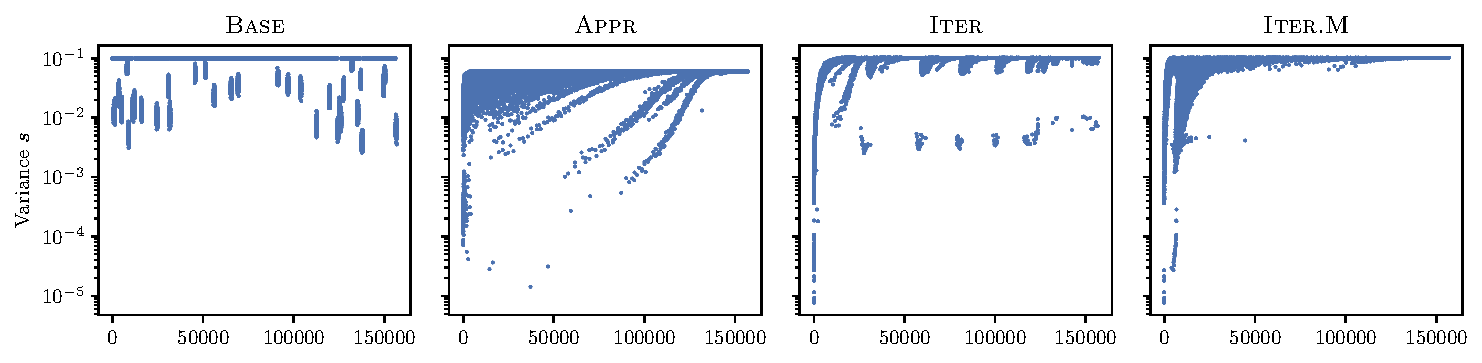
\includegraphics[width=\textwidth]{Figures/PacBayes/FC2_10cls/sigma_post_compare_iter_iterH_Sigma_post_MNIST_Exp1FC2_fixlr0.01_fc1.weight.pdf}
    % \captionsetup{justification=centering}
    \caption{Optimized posterior variance, $\vs$. (fc1:T-$200^2$, trained on MNIST), the horizontal axis is ordered with decreasing eigenvalues.}
    \label{fig:app_PAC}
\end{figure}

\newpage



\begin{table}[H]
  \centering
  \caption{Full PAC-Bayes bound optimization results}
  \vskip 0.1in
    \begin{center}
    \begin{tabular}{llccccc}
    \toprule
    \textbf{Network} & \textbf{Method} &  \shortstack{PAC-Bayes\\Bound} & \shortstack{KL\\Divergence} & \shortstack{SNN\\loss} & \shortstack{$\lambda$ (prior)} &\shortstack{Test\\Error} 
    \\ \midrule
    T-600          & \textsc{Prev}         & 0.161  & 5144   & 0.028   &    -    & 0.017 \\
                   & \textsc{Base}      & 0.154  & 4612.6 & 0.03373 & -1.3313 & 0.0153 \\
                   & \textsc{Appr}     & 0.1432 & 3980.6 & 0.03417 & -1.6063 & 0.0153 \\
                   & \textsc{Iter}       & \textbf{0.1198} & 3766.1 & 0.02347 & -1.2913 & 0.0153 \\
                   & \textsc{Iter(D)} & 0.1199 & 3751.1 & 0.02366 & -1.2913 & 0.0153 \\
                   & \textsc{Iter.M} & 0.1255 & 3929.9 & 0.02494 & -1.3213 & 0.0153\\
    \hline\rule{0pt}{2.5ex}
    T-$600^2$      & \textsc{Prev}        & 0.186  & 6534   & 0.028   &    -    & 0.016 \\
                   & \textsc{Base}      & 0.1921 & 6966.6 & 0.03262 & -1.4163 & 0.0148 \\
                   & \textsc{Appr}     & 0.1658 & 5176.1 & 0.03468 & -2.0963 & 0.0148 \\
                   & \textsc{Iter}       & 0.1456 & 5086.5 & 0.02473 & -1.7963 & 0.0148 \\
                   & \textsc{Iter(D)} & \textbf{0.1443} & 4956.8 & 0.02523 & -1.7963 & 0.0148 \\
                   & \textsc{Iter.M} & 0.1502 & 5024.5 & 0.02767 & -1.8363 & 0.0148\\
    \hline\rule{0pt}{2.5ex}
    
    
    T-1200         & \textsc{Prev}         & 0.179  & 5977   & 0.027   &    -    & 0.016 \\
                   & \textsc{Base}      & 0.1754 & 5917.6 & 0.03295 & -1.5463 & 0.0161 \\
                   & \textsc{Appr}     & 0.1725 & 5318.8 & 0.03701 & -1.8313 & 0.0161 \\
                   & \textsc{Iter}       & 0.1417 & 5071  & 0.02292 & -1.4763 & 0.0161 \\
                   & \textsc{Iter(D)} & \textbf{0.1413} & 5021.1 & 0.02316 & -1.4763 & 0.0161 \\
                   & \textsc{Iter.M} & 0.1493 & 5185.4 & 0.02576	& -1.5363 &	0.0161\\
    \hline\rule{0pt}{2.5ex}
    T-$300^2$      & \textsc{Prev}         & 0.17   & 5791   & 0.027   &    -    & 0.015 \\
                   & \textsc{Base}      & 0.1686 & 5514.9 & 0.03329 & -1.1513 & 0.015 \\
                   & \textsc{Appr}     & 0.1434 & 4105.4 & 0.03296 & -1.8063 & 0.015 \\
                   & \textsc{Iter}       & 0.1249 & 3873.2 & 0.02514 & -1.4763 & 0.015 \\
                   & \textsc{Iter(D)} & \textbf{0.1244} & 3833.7 & 0.02526 & -1.4763 & 0.015 \\
                   & \textsc{Iter.M} & 0.1308	& 3987.2 &	0.02721	 & -1.5713 & 0.015 \\
    \hline\rule{0pt}{2.5ex}
    R-600          & \textsc{Prev}         & 1.352  & 201131 & 0.112   &    -    & 0.501 \\
                   & \textsc{Base}      & 0.6046 & 1144.8 & 0.507   & -1.8263 & 0.4925 \\
                   & \textsc{Appr}     & 0.5653 & 390.25 & 0.5066  & -2.4713 & 0.4925 \\
                   & \textsc{Iter(D)} & 0.5681 & 431.62 & 0.5066  & -2.4513 & 0.4925 \\
                   & \textsc{Iter.M} & \textbf{0.5616} & 340.62 &	0.5065	& -2.5263 &	0.4925\\
    \hline\rule{0pt}{2.5ex}
    T-$200^2_{10}$     & \textsc{Base}      & 0.4165 & 21896  & 0.04706 & -1.1513 & 0.0208 \\
                   & \textsc{Appr}     & 0.2621 & 11068  & 0.0366  & -1.4213 & 0.0208 \\
                   & \textsc{Iter}       & \textbf{0.2145} & 9821  & 0.02229 & -1.1513 & 0.0208 \\
                   & \textsc{Iter(D)} & 0.2311 & 9758.5 & 0.03071 & -1.1513 & 0.0208 \\
                   & \textsc{Iter.M} & 0.2728 & 13406 & 0.02605	& -1.1513 &	0.0208\\
    \hline\rule{0pt}{2.5ex}
    T-$600_{10}$   & \textsc{Base}      & 0.2879 & 12674  & 0.03854 & -1.1513 & 0.018 \\
                   & \textsc{Appr}     & 0.2424 & 9095.8 & 0.04159 & -1.6013 & 0.018 \\
                   & \textsc{Iter}       & \textbf{0.2132} & 8697.9 & 0.02947 & -1.3063 & 0.018 \\
                   & \textsc{Iter.M} & 0.2227	& 8870.9	& 0.03294	& -1.4613	& 0.018 \\
    \hline\rule{0pt}{2.5ex}
    T-$600^2_{10}$ & \textsc{Base}      & 0.3472 & 17212  & 0.03884 & -1.1513 & 0.0186 \\
                   & \textsc{Appr}     & 0.2896 & 11618  & 0.04723 & -2.0563 & 0.0186 \\
                   & \textsc{Iter}       & \textbf{0.2431} & 10568 & 0.03057 & -1.5713 & 0.0186 \\
    \bottomrule
    \end{tabular}
\end{center}
  \label{tab:app_pac}
\end{table}


\section{Limitations and Conclusions}
%!TEX root = stability_manifold_TSP.tex
In this paper, we have defined manifold convolutions and manifold neural networks. We prove that the deformations on the embedded submanifolds can be represented as a form of perturbations to the Laplace-Beltrami operator. Considering the infinite dimensionality of LB operators, we import the definition of frequency difference threshold filters and frequency ratio threshold filters to help separate the spectrum. By assigning similar frequency responses to the eigenvalues that are close enough, these filters can be proved to be stable under absolute and relative perturbations to the LB operator respectively with Lipschitz continuous assumptions. While the manifold filters need to trade-off between the stability and discriminability.  MNNs composed with layers of manifold filters and pointwise nonlinearities can be proved to be stable to absolute and relative perturbations to the LB operators. While the frequency mixing brought by pointwise nonlinearity can help with the discriminability. We conclude that the MNNs are thus both stable to deformations and discriminative. We also show the discretizations of MNNs in both spatial and time domains to make our proposed MNNs implementable. 
We finally verified our results numerically with a point cloud classification problem with ModelNet10 dataset.

\bibliography{VOLDNN_arXiv}
\bibliographystyle{icml2021}

%%%%%%%%%%%%%%%%%%%%%%%%%%%%%%%%%%%%%%%%%%%%%%%%%%%%%%%%%%%%

\appendix

\section{Detailed Derivations}
\label{sec:appendix_derivation_main}
\subsection{Derivation of Hessian}
\label{sec:appendix_derivation}
For an input $\vx$ with label $\vy$, we define the Hessian of single input loss with respect to vector $\vv$ as
\begin{equation}
    \mH_\ell(\vv, \vx) = \nabla^2_\vv \ell(f_\vtheta(\vx), \vy) = \nabla^2_\vv \ell(\zx, \vy).
\end{equation}
We define the Hessian of loss with respect to $\vv$ for the entire training sample as
\begin{equation}
   \HessL(\vv) = \nabla^2_\vv\Ls(\vtheta) = \sum_{i=1}^N \nabla^2_\vv \ell(f_\vtheta(\vx_i), \vy_i)= \sum_{i=1}^N \mH_\ell(\vv, \vx_i) = \E\left[ \mH_\ell(\vv, \vx)\right].
\end{equation}
We now derive the Hessian for a fixed input label pair ($\vx, \vy$). Following the definition and notations in \sectionref{sec:prelim}, we also denote output as $\vz = f_\vtheta(\vx)$. We fix a layer $p$ for the layer-wise Hessian. Here the layer-wise weight Hessian is $\mH_\ell(\vw^{(p)}, \vx)$. We also have the output for the layer as $\vz^{(p)}$. Since $\vw^{(p)}$ only appear in the layer but not the subsequent layers, we can consider $ \vz = f_\vtheta(\vx) = g_\vtheta(\vz^{(p)}(\vw,\vx))$ where $g_\vtheta$ only contains the layers after the $p$-th layer and does not depend on $\vw^{(p)}$. Thus, using the Hessian Chain rule \citep{skorski2019chain}, we have 
\begin{equation}
    \mH_\ell(\vw^{(p)}, \vx) = \left(\frac{\partial \vz^{(p)}}{\partial\vw^{(p)}}\right)^\T\mH_\ell(\vz^{(p)}, \vx)\left(\frac{\partial \vz^{(p)}}{\partial\vw^{(p)}}\right) + \sum_{i=1}^{m^{(p)}} \frac{\partial \ell(\vz, \vy)}{\partial\evz_i^{(p)}} \nabla^2_{\vw^{(p)}} \evz_i^{(p)},
\end{equation}
where $\evz_i^{(p)}$ is the $i$th entry of $\vz^{(p)}$ and $m^{(p)}$ is the number of neurons in $p$-th layer (size of $\vz^{(p)}$).

Since $\vz^{(p)} = \mW^{(p)}\vx^{(p)} + \vb^{(p)}$ and $\vw^{(p)} = \vect(\mW^{(p)})$ we have
\begin{equation}
    \frac{\partial \vz^{(p)}}{\partial\vw^{(p)}} = \mI_{m^{(p)}} \otimes \vx^{(p)\T}.
\end{equation}
Since $\frac{\partial \vz^{(p)}}{\partial\vw^{(p)}}$ does not depend on $\vw^{(p)}$, for all $i$ we have $\nabla^2_{\vw^{(p)}} \evz_i^{(p)} = 0$.
Thus, \begin{equation}
    \mH_\ell(\vw^{(p)}, \vx) = \left(\mI_{m^{(p)}} \otimes \vx^{(p)}\right)\mH_\ell(\vz^{(p)}, \vx)\left(\mI_{m^{(p)}} \otimes \vx^{(p)\T}\right).
\end{equation}
We define $\mM^{(p)}_\vx = \mH_\ell(\vz^{(p)}, \vx)$ as in \sectionref{sec:prelim} so that \begin{equation}
    \mH_\ell(\vw^{(p)}, \vx) = \left(\mI_{m^{(p)}} \otimes \vx^{(p)}\right)\mM^{(p)}_\vx\left(\mI_{m^{(p)}} \otimes \vx^{(p)\T}\right) = \mM_\vx^{(p)} \otimes \vx^{(p)}\vx^{(p)\T}.
    \label{eqn:appendix_closeformhessian}
\end{equation}

We now look into $\mM_x^{(p)} = \mH_\ell(\vz^{(p)}, \vx)$. Again we have $\vz = g_\vtheta(\vz^{(p)})$ and can use chain rule here,
\begin{equation}
    \mH_\ell(\vz^{(p)}, \vx) = \left(\frac{\partial \vz}{\partial\vz^{(p)}}\right)^\T\mH_\ell(\vz, \vx)\left(\frac{\partial \vz}{\partial\vz^{(p)}}\right) + \sum_{i=1}^{c} \frac{\partial \ell(\vz, \vy)}{\partial\evz_i} \nabla^2_{\vz^{(p)}} \evz_i
\end{equation}
By letting $\vp := \softmax(\vz)$ be the output confidence vector, we define the Hessian with respect to output logit $\vz$ as $\mA_\vx$ and have
\begin{equation}
    \label{eqn:hessian_decomp_general}
    \mA_\vx := \mH_\ell(\vz, \vx) = \nabla^2_\vz l(\vz,\vy)= \diag(\vp)- \vp\vp^\T,
\end{equation}
according to \citet{singla2019understanding}.

We also define the Jacobian of $\vz$ with respect to $\vz^{(p)}$ (informally logit gradient for layer $p$) as $\mG^{(p)}_\vx := \frac{\partial \vz}{\partial\vz^{(p)}}$.
For FC layers with ReLUs, we can consider ReLU after the $p$-th layer as multiplying $\vz^{(p)}$ by an indicator function $\1_{\vz^{(p)} > 0}$. To use matrix multiplication, we can turn the indicator function into a diagonal matrix and define it as $\mD^{(p)}$ where
\begin{equation}
    \mD^{(p)} := \diag\left(\1_{\vz^{(p)} > 0}\right).
\end{equation}
Thus, we have the input of the next layer as $\vx^{(p+1)} = \mD^{(p)}\vz^{(p)}$.
The FC layers can then be considered as a sequential matrix multiplication and we have the final output as
\begin{equation}
    \vz = \mW^{(L)}\mD^{(L-1)}\mW^{(L-1)}\mD^{(L-2)}\cdots \mD^{(p)}\vz^{(p)}.
\end{equation}
Thus, \begin{equation}
    \mG_\vx^{(p)} = \frac{\partial \vz}{\partial\vz^{(p)}} = \mW^{(L)}\mD^{(L-1)}\mW^{(L-1)}\mD^{(L-2)}\cdots \mD^{(p)}.
\end{equation}
Since $\mG_\vx^{(p)}$ is independent of $\vz^{(p)}$, we have
\begin{equation}
    \nabla^2_{\vz^{(p)}} \evz_i = 0, \forall i.
    \label{eqn:appendix_zero_logit_output_hessian}
\end{equation}
Thus, \begin{equation}
    \mM_\vx^{(p)} = \mH_\ell(\vz^{(p)}, \vx) = \mG_\vx^{(p)\T}\mA_\vx\mG_\vx^{(p)}.
\end{equation}
Moreover, loss Hessian with respect to the bias term $\vb^{(p)}$ equals to that with respect to the output of that layer $\vz^{(p)}$. We thus have
\begin{equation}
    \mH_\ell(\vb^{(p)}, \vx) = \mM_\vx^{(p)} = \mG_\vx^{(p)\T}\mA_\vx\mG_\vx^{(p)}.
\end{equation}

The Hessians of loss for the entire training sample are simply the empirical expectations of the Hessian for single input. We have the formula as the following:
\begin{align}
    \HessL(\vw^{(p)}) &= \E\left[\mH_\ell(\vw^{(p)}, \vx)\right] = \E\left[\mM^{(p)}_\vx \otimes \vx^{(p)}\vx^{(p)\T}\right],\label{eqn:app_layerwise_approx}\\
    \HessL(\vb^{(p)}) &= \HessL(\vz^{(p)}) = \E\left[\mM^{(p)}_\vx\right] = \E\left[\mG_\vx^{(p)\T}\mA_\vx\mG_\vx^{(p)}\right].
\end{align}

Note that we can further decompose $\mA_\vx = \mQ_\vx^\T\mQ_\vx$, where 
\begin{equation}
    \Qx = \diag\left(\sqrt{\vp}\right)\left(\mI_c-\1_c\vp^\T\right),
    \label{eqn:app_qx}
\end{equation}
with $\1_c$ is a all one vector of size $c$, proved in \citet{papyan2019measurements}.

We can further extend the close form expression to off diagonal blocks and the bias entries to get the full Gauss-Newton term of Hessian. Let
\begin{align}
    \mF^\T_\vx = \begin{pmatrix}
    \Gx^{(1)\T} \otimes \vx^{(1)}\\
    \Gx^{(1)\T}\\
    \Gx^{(2)\T} \otimes \vx^{(2)}\\
    \Gx^{(2)\T}\\
    \vdots\\
    \Gx^{(L)\T} \otimes \vx^{(n)}\\
    \Gx^{(L)\T}
    \end{pmatrix}.
\end{align}
The full Hessian is given by
\begin{equation}
    \HessL(\vtheta) = \E \left[\mF^\T_{\vx}\mA_\vx\mF_{\vx}\right] + \E\left[\sum_{i=1}^c \frac{\partial \ell(\vz,\vy)}{\evz_i} \nabla^2_\vtheta \evz_i \right].
\label{eqn:app_full_hessian}
\end{equation}
\subsection{Approximating Weight Hessian of Convolutional Layers}
\label{sec:appendix_conv}
The approximation of weight Hessian of convolutional layer is a trivial extension from the approximation of Fisher information matrix of convolutional layer by \citet{grosse2016kronecker}.

Consider a two dimensional convolutional layer of neural network with $m$ input channels and $n$ output channels. Let its input feature map $\tX$ be of shape $(n, X_1, X_2)$ and output feature map $\tZ$ be of shape $(m, P_1, P_2)$. Let its convolution kernel be of size $K_1\times K_2$. Then the weight $\tW$ is of shape $(m, n, K_1, K_2)$, and the bias $\vb$ is of shape $(m)$. Let $P$ be the number of patches slide over by the convolution kernel, we have $P=P_1P_2$.

Follow  \citet{dangel2020modular}, we define $\mZ\in\R^{m\times P}$ as the reshaped matrix of $\tZ$ and $\mW\in\R^{m \times nK_1K_2}$ as the reshaped matrix of $\tW.$
Define $\mB\in\R^{m\times P}$ by broadcasting $\vb$ to $P$ dimensions. Let $\mX\in\R^{nK_1K_2 \times P}$ be the unfolded $\tX$ with respect to the convolutional layer. The unfold operation \citep{NEURIPS2019_9015} is commonly used in computation to model convolution as matrix operations.

After the above transformation, we have the linear expression of the $p$-th convolutional layer similar to FC layers:\begin{equation}
    \label{eqn:conv_linear}
    \mZ^{(p)} = \mW^{(p)}\mX^{(p)} + \mB^{(p)}
\end{equation}
We still omit superscription of $(p)$ for dimensions for simplicity. We also denote $\vz^{(p)}$ as the vector form of $\mZ^{(p)}$ and has size $mP$.
Similar to fully connected layer, we have analogue of \equationref{eqn:appendix_closeformhessian} for convolutional layer as
\begin{equation}
    \label{eqn:appendix_closeformhessian_conv}
    \mH_\ell(\vw^{(p)}, \mX) = \left(\mI_{m} \otimes \mX^{(p)}\right)\mM_\vx^{(p)}\left(\mI_{m} \otimes \mX^{(p)\T}\right),
\end{equation}
where $\mM_\vx^{(p)} = \mH_\ell(\vz^{(p)}, \mX)$ and is a $mP \times mP$ matrix.
Also, since convolutional layers can also be considered as linear operations (matrix multiplication with reshape) together with FC layers and ReLUs, \equationref{eqn:appendix_zero_logit_output_hessian} still holds. Thus, we still have  \begin{equation}
    \mH_\ell(\vz^{(p)}, \mX) = \mM_\vx^{(p)} = \mG_\vx^{(p)\T}\mA_\vx\mG_\vx^{(p)},
\end{equation}
where $\mG_\vx^{(p)} = \frac{\partial \vz}{\partial\vz^{(p)}}$ and has dimension $c \times mP$, although is cannot be further decomposed as direct multiplication of weight matrices as in the FC layers.

However, for convolutional layers, $\mX^{(p)}$ is a matrix instead of a vector. Thus, we cannot make \equationref{eqn:appendix_closeformhessian_conv} into the form of a Kronecker product as in \equationref{eqn:appendix_closeformhessian}.

Despite this, it is still possible to have a Kronecker factorization of the weight Hessian in the form
\begin{equation}
   \mH_\ell(\vw^{(p)}, \mX) \approx \tmM^{(p)}_\vx \otimes \mX^{(p)}\mX^{(p)\T},
\end{equation}
using further approximation motivated by \cite{grosse2016kronecker}.
Note that $\tmM^{(p)}_\vx$ need to have a different shape ($m\times m$) from $\mM^{(p)}_\vx$ ($mP\times mP$), since $\mH_\ell(\vw^{(p)},\mX)$ is $mnK1K2 \times mnK1K2$ and $\mX^{(p)}\mX^{(p)\T}$ is $nK1K2 \times nK1K2$.

Since we can further decompose $\Ax = \Qx^\T\Qx$, we then have
\begin{equation}
    \Mx^{(p)} = \mG_\vx^{(p)\T}\Ax\mG_\vx^{(p)} = \left(\Qx\Gx^{(p)}\right)^\T\left(\Qx\Gx^{(p)}\right).
\end{equation}
We define $\mN_\vx^{(p)} =\Qx\Gx^{(p)}$. Here $\Qx$ is $c\times c$ and $\Gx^{(p)}$ is $c\times mP$ so that $\mN_\vx^{(p)}$ is $c \times mP$. We can reshape $\mN_\vx^{(p)}$ into a $cP\times m$ matrix $\tmN_\vx^{(p)}$. We then reduce $\mM^{(p)}_\vx$ ($mP\times mP$) into a $m\times m$ matrix as 
\begin{equation}
    \tmM^{(p)}_\vx = \frac{1}{P}\tmN_\vx^{(p)\T}\tmN_\vx^{(p)}.
\end{equation}
The scalar $\frac{1}{P}$ is a normalization factor since we squeeze a dimension of size $P$ into size 1.

Thus, we can have similar Kronecker factorization approximation as
\begin{align}
    \HessL(\vw^{(p)}) &= \E\left[\mH_\ell(\vw^{(p)}, \mX)\right] = 
    \E\left[\left(\mI_{m} \otimes \mX^{(p)}\right)\mM_\vx^{(p)}\left(\mI_{m} \otimes \mX^{(p)\T}\right)\right] \\ &\approx \E\left[\tmM^{(p)}_\vx \otimes \mX^{(p)}\mX^{(p)\T}\right] \approx \E\left[\tmM^{(p)}_\vx\right] \otimes \E\left[\mX^{(p)}\mX^{(p)\T}\right].
\end{align}
\newpage
\section{Main Proof}
\label{sec:main-proof-full}
This is the complete proof for the two main theorems sketched in \sectionref{sec:theoretical}.
\subsection{Preliminaries}
\label{sec:proof-prelim}
\subsubsection{Notations}
In this section, we generally follow the notation standard by \citet{goodfellow2016deep}. We will use bold italic lowercase letters ($\vv$) to denote vectors, bold non-italic lowercase letters to denote random vectors ($\rvv$), bold italic uppercase letters ($\mA$) to denote matrices, and bold italic uppercase letters ($\rmA$) to denote random matrices.

Moreover, we use $[n]$ for positive integer $n$ to denote the set $\{1,\cdots,n\}$, and $\norm{\mM}$ to denote the spectral norm of a matrix $\mM$. We use $\innerf{\mA, \mB}$ to denote the Frobenius inner product of two matrices $\mA$ and $\mB$, namely $\innerf{\mA, \mB} \triangleq\sum_{i,j}\mA_{i,j}\mB_{i,j}$. We use $\tr(\mM)$ to denote the trace of a matrix $\mM$, and we use $\textbf{1}_c$ to denote the all-one vector of dimension $c$ (the subscript may be omitted when it's clear from the context).

For probability distributions, we use $\rectNormal(\mu,\sigma)$ to denote the rectified Gaussian distribution which has density function\begin{equation}
    f_\rectNormal(x;\mu,\sigma) = \Phi\rbr{\frac\mu\sigma}\delta(x)+\frac{1}{\sqrt{2\pi\sigma^2}}\exp\rbr{-\frac{(x-\mu)^2}{2\sigma^2}}\ind\sbr{x> 0}.
\end{equation}
Here $\Phi$ is the CDF of standard normal distribution, $\delta(x)$ is the Dirac delta function. Note that when $\mu=0$, the density function simplifies to\begin{align}
    f_\rectNormal(x;0,\sigma) = 
    \frac12\delta(x)+\frac{1}{\sqrt{2\pi\sigma^2}}\exp\rbr{-\frac{x^2}{2\sigma^2}}\ind\sbr{x> 0}.
\end{align}
We will use the same notation for multivariate rectified Gaussian distribution, which will be used to characterize the inputs of the network.
% \znote{Move this to somewhere after we define the network?}
\subsubsection{Problem Setting}

Consider a two layer fully connected ReLU activated neural network with input dimension $d$, hidden layer dimension $n$ and output dimension $c$. In particular, $n$ goes to infinity, $d=n^{1+\alpha}$ for some $\alpha>0$, and $c$ is a finite constant. Let network be trained with cross-entropy objective $\gL$. Let $\sigma$ denote the element-wise ReLU activation function which acts as $\sigma(x) = x\cdot\ind_{x\geq 0}$ and the product here is applied element-wise.
Let $\mW^{(1)}\in\R^{n\times d}$ and $\mW^{(2)}\in\R^{c\times n}$ denote the weight matrices of the first and second layer respectively. 
%Let $\vb^{(1)}\in\R^{n}$ and $\vb^{(2)}\in\R^{c}$ denote the weight matrices of the first and second layer respectively.

We consider the case that the neural network has rectified standard Gaussian input $\rvx\sim \rectNormal(0, \mI_d)$. 
Denote the output of the first and second layer as $\rvy$ and $\rvz$ respectively. We have $\rvy = \sigma(\mW^{(1)}\rvx)$ and $\rvz = \mW^{(2)}\rvy.$ Let $\rvp=\mbox{softmax}(\rvz)$ denote the softmax output of the network and let $\rmA\triangleq\diag(\rvp)-\rvp\rvp^\T$.

In this problem, we look into the state of random Gaussian initialization, in which entries of both matrices are i.i.d. sampled from a standard normal distribution, and then re-scaled such that each row of $\mW^{(1)}$ and $\mW^{(2)}$ has norm 1. When taking $n$ and $d$ to infinity, with the concentration of norm in high-dimensional Gaussian random variables, we assume in this problem that entries of $\mW^{(1)}$ are iid sampled from a zero-mean distribution with variance $1/d$, and entries of $\mW^{(2)}$ are iid sampled from a zero-mean distribution with variance $1/n$. This initialization is standard in training neural networks. From the previous analysis of Hessian, the output Hessian corresponding to the first layer has closed form
\begin{equation}
    \mM^{(1)} \triangleq \exop{\rvx\sim \rectNormal(0, \mI_d)}{\rmD\mW^{(2)\\T}\rmA\mW^{(2)}\rmD},
\end{equation}
where $\rmD\triangleq\diag(\ind\sbr{\rvy\geq 0})\in\R^{n\times n}$ is the random 0/1 diagonal matrix representing the activations of ReLU function after the first layer. Note that the output Hessian of the second layer is simply $\mM^{(2)}\triangleq\ex{\rmA}$.

By the Kronecker decomposition, the closed form of the layer-wise Hessians of the first and the second layer are\begin{align*}
    \mH^{(1)} &\triangleq \exop{\rvx\sim \rectNormal(0, \mI_d)}{\rmD\mW^{(2)\T}\rmA\mW^{(2)}\rmD\otimes \rvx\rvx^\T},\\
    \mH^{(2)} &\triangleq \exop{\rvx\sim \rectNormal(0, \mI_d)}{\rmA\otimes \rmD\mW^{(1)}\rvx\rvx^\T\mW^{(1)\T}\rmD}.
\end{align*}
Following the decoupling conjecture, let the Kronecker approximation of the Hessians above be\begin{align*}
    \hat\mH^{(1)} &\triangleq \exop{\rvx\sim \rectNormal(0, \mI_d)}{\rmD\mW^{(2)\T}\rmA\mW^{(2)}\rmD}\otimes\exop{\rvx\sim \rectNormal(0, \mI_d)}{\rvx\rvx^\T},\\
    \hat\mH^{(2)} &\triangleq \exop{\rvx\sim \rectNormal(0, \mI_d)}{\rmA}\otimes\exop{\rvx\sim \rectNormal(0, \mI_d)}{\rmD\mW^{(1)}\rvx\rvx^\T\mW^{(1)\T}\rmD}.
\end{align*}
The decoupling conjecture is then equivalent to $\mH^{(1)}\approx \hat\mH^{(1)}$, $\mH^{(2)}\approx \hat\mH^{(2)}$.

Since our formulae for the Hessians are going to depend on the weight matrices, throughout the section we will condition on the value of $\mW^{(1)}$ and $\mW^{(2)}$ when we take expectation (i.e. the expectation is only taken over the input $\rvx\sim \rectNormal(0, \mI_d)$). We will neglect this under-script of the expectation operator $\E$ as there will be no confusion. When we are discussing the Hessians of a certain layer, we will also neglect the upper-script and just use $\mH$ and $\mM$ when there is no confusion. Moreover, we denote $\rmX\triangleq\ex{\rvx\rvx^\T}$ as the autocorrelation of the input.

Furthermore, for simplicity of notations, we will sometimes use the verbal description ``with probability 1 over $\mW^{(1)}$/$\mW^{(2)}$, event $E$ is true'' to denote
\begin{equation}
    \lim_{n\to\infty}\prop{\mW^{(1)}\sim\gN(0,\frac{1}{d}\mI_{nd}), \mW^{(2)}\sim\gN(0,\frac{1}{n}\mI_{cn})}{E} = 1.
\end{equation}

% \newpage
\subsection{Detailed Proof}
\label{sec:detailed-proof}
\input{MainProof/main-theorems}
\input{MainProof/w-properties}
\input{MainProof/approx-independence}
\input{MainProof/A-structure}
\input{MainProof/projection-approx}
\input{MainProof/out-hessian-structure}
\input{MainProof/full-hessian-structure}
\newpage
\section{Structure of Dominating Eigenvectors of the Full Hessian.}

% \znote{should we move thiis section to an earlier place?}
\label{sec:appendix_full_hessian}
Although it is not possible to apply Kronecker factorization to the full Hessian directly, we can construct an approximation of the top eigenvectors and eigenspace using similar ideas and our findings.In this section, we will always have superscript $(p)$ for all layer-wise matrices and vectors in order to distinguish them from the full versions.
As shown in \equationref{eqn:app_full_hessian} of \sectionref{sec:appendix_derivation}, we have the full Hessian of fully connected networks as 
\begin{equation}
    \HessL(\vtheta) = \E \left[\mF^\T_{\vx}\mA_\vx\mF_{\vx}\right] + \E\left[\sum_{i=1}^c \frac{\partial \ell(\vz,\vy)}{\evz_i} \nabla^2_\vtheta \evz_i \right],
\label{eqn:app_full_hessian_2}
\end{equation}
where
\begin{align}
    \mF^\T_\vx = \begin{pmatrix}
    \Gx^{(1)\T} \otimes \vx^{(1)}\\
    \Gx^{(1)\T}\\
    \Gx^{(2)\T} \otimes \vx^{(2)}\\
    \Gx^{(2)\T}\\
    \vdots\\
    \Gx^{(L)\T} \otimes \vx^{(n)}\\
    \Gx^{(L)\T}
    \end{pmatrix}.
\end{align}
In order to simplify the formula, we define \begin{equation}
    \tilde{\vx}^{(p)} = \begin{pmatrix}
    \vx^{(p)}\\
    1
    \end{pmatrix}
\end{equation} to be the extended input of the $p$-th layer. Thus, the terms in the Hessian attributed to the bias can be included in the Kronecker product with the extended input, and $\mF_\vx^\T$ can be simplified as
\begin{align}
\label{eqn:app_f_extened}
    \mF^\T_\vx = \begin{pmatrix}
    \Gx^{(1)\T} \otimes \tilde{\vx}^{(1)}\\
    \Gx^{(2)\T} \otimes \tilde{\vx}^{(2)}\\
    \vdots\\
    \Gx^{(L)\T} \otimes \tilde{\vx}^{(n)}\\
    \end{pmatrix}.
\end{align}

As discussed in several previous works \citep{sagun2016eigenvalues, papyan2018full, papyan2019measurements, fort2019emergent}, the full Hessian can be decomposed in to the G-term and the H-term. Specifically, the G-term is $\E \left[\mF^\T_{\vx}\mA_\vx\mF_{\vx}\right]$, and the H-term is $\E\left[\sum_{i=1}^c \frac{\partial \ell(\vz,\vy)}{\evz_i} \nabla^2_\vtheta \evz_i \right]$ in \equationref{eqn:app_full_hessian_2}.

Empirically, the G-term usually dominates the H-term, and the top eigenvalues and eigenspace of the Hessian are mainly attributed to the G-term. Since we focus on the top eigenspace, we can approximate our full Hessian using the G-term, as
\begin{equation}
     \HessL(\vtheta) \approx  \E\left[\mF^\T_{\vx}\mA_\vx\mF_{\vx}\right].
\end{equation}

In our approximation of the layer-wise Hessian $\HessL(\vw^{(p)})$ \equationref{eqn:decomp}, the two parts of the Kronecker factorization are the layer-wise output Hessian $\E[\mM^{(p)}_\vx]$ and the auto-correlation matrix of the input $\E[\vx^{(p)}\vx^{(p)\T}]$. Although we cannot apply Kronecker factorization to $\E\left[\mF^\T_{\vx}\mA_\vx\mF_{\vx}\right]$, we can still approximate its eigenspace using the eigenspace of the full output Hessian.

Note here that the full output Hessian is not a common definition. Let $\hat{m} = \sum_{p=1}^Lm^{(p)}$ be the sum of output dimension of each layer. We define a full output vector $\tilde{\vz}\in\R^{\hat{m}}$ by concatenating all the layerwise outputs together,
\begin{equation}
    \tilde{\vz} := \begin{pmatrix}
    \vz^{(1)}\\
    \vz^{(2)}\\
    \vdots\\
    \vz^{(L)}
    \end{pmatrix}.
\end{equation} 
We then define the full output Hessian is the Hessian w.r.t. $\tilde{\vz}$. Let the full output Hessian for a single input $\vx$ be $\mM_\vx\in\R^{\hat{m}\times \hat{m}}$. Similar to \equationref{eqn:app_layerwise_approx}, it can be expressed as
\begin{equation}
    \mM_\vx := \mH_\ell(\tilde{\vz}, \vx) = \mG_\vx^{\T}\mA_\vx\mG_\vx,
\end{equation}
where
\begin{equation}
    \mG^\T_\vx = \begin{pmatrix}
    \mG_\vx^{(1)\T}\\
    \mG_\vx^{(2)\T}\\
    \vdots\\
    \mG_\vx^{(L)\T}
    \end{pmatrix}
\end{equation}
similar to \equationref{eqn:app_f_extened}.
The full output Hessian for the entire training sample is thus
\begin{equation}
    \HessL(\tilde{\vz}) = \E[\mM_\vx] = \E[\mG_\vx^{\T}\mA_\vx\mG_\vx].
\end{equation}

We can then approximate the eigenvectors of the full Hessian $\HessL(\vtheta)$ using the eigenvectors of $\E[\mM_\vx]$. Let the $i$-th eigenvector of $\HessL(\vtheta)$ be $\vv_i$ and that of $\E[\mM_\vx]$ be $\vu_i$. We may then break up $\vu_i$ into segments corresponding to different layers as in
\begin{equation}
    \vu_i = \begin{pmatrix}
    \vu_i^{(1)}\\
    \vu_i^{(2)}\\
    \vdots\\
    \vu_i^{(L)}
    \end{pmatrix},
\end{equation}
where for all layer $p$, $\vu_i^{(p)}\in\R^{m^{(p)}}$.
Motivated by the relation between $\mG_\vx$ and $\mF_\vx$, the $i$-th eigenvector of $\HessL(\vtheta)$ can be approximated as the following. Let
\begin{equation}
    \vw_i = \begin{pmatrix}
    \vu_i^{(1)} \otimes \E[\tilde{\vx^{(1)}}]\\
    \vu_i^{(2)}\otimes \E[\tilde{\vx^{(2)}}]\\
    \vdots\\
    \vu_i^{(L)}\otimes \E[\tilde{\vx^{(L)}}]
    \end{pmatrix}.
\end{equation}
We then have
\begin{equation}
    \vv_i \approx \frac{\vw_i}{\|\vw_i\|}
\end{equation}
We can then use the Gram–Schmidt process to get the basis vectors of the approximated eigenspace.

Another reason for this approximation is that the expectation is the input of each layer $\E[\vx^{(p)}]$ dominates its covariance as shown in \sectionref{sec:appendix_xxT}. Thus, the approximate is accurate for top eigenvectors and also top eigenspace. For latter eigenvectors, the approximation would not be as accurate since this approximate loses all information in the covariance of the inputs.

We also approximated the eigenvalues using this approximation. Let the $i$-th eigenvalue of $\HessL(\vtheta)$ be $\lambda_i$ and that of $\E[\mM_\vx]$ be $\sigma_i$. We have
\begin{equation}
    \lambda_i \approx \sigma_i\|\vw_i\|^2.
\end{equation}

Below we show the approximation of the eigenvalues top eigenspace using this method. The eigenspace overlap is defined as in \definitionref{def:overlap}. We experimented on several fully connected networks, the results shown below are for F-$200^2$ (same as  \figureref{fig:eigeninfo_approx}(c)(d) in the main text), F-$200^4$, F-$600^4$, and F-$600^8$, all with dimension 50. The approximations are reasonably accurate.

\begin{figure}[H]
    \centering
    \begin{subfigure}[t]{0.5\textwidth}
        \centering
        \captionsetup{justification=centering}
        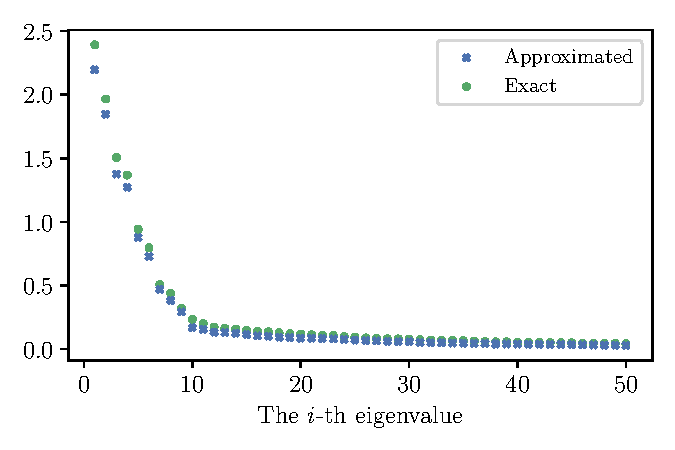
\includegraphics[width=\textwidth]{Appendix_Figures/Full_hessian/newplots/eigenval_fc2_200.pdf}
        \caption{Eigenvalues for F-$200^2$}
    \end{subfigure}%
    \begin{subfigure}[t]{0.5\textwidth}
        \centering
        \captionsetup{justification=centering}
        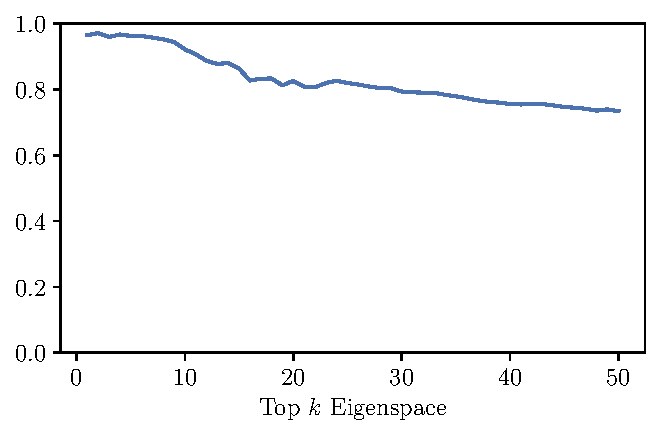
\includegraphics[width=\textwidth]{Appendix_Figures/Full_hessian/newplots/eigenvec_fc2_200.pdf}
        \caption{Eigenspace overlap for F-$200^2$}
    \end{subfigure}\\
    \begin{subfigure}[t]{0.5\textwidth}
        \centering
        \captionsetup{justification=centering}
        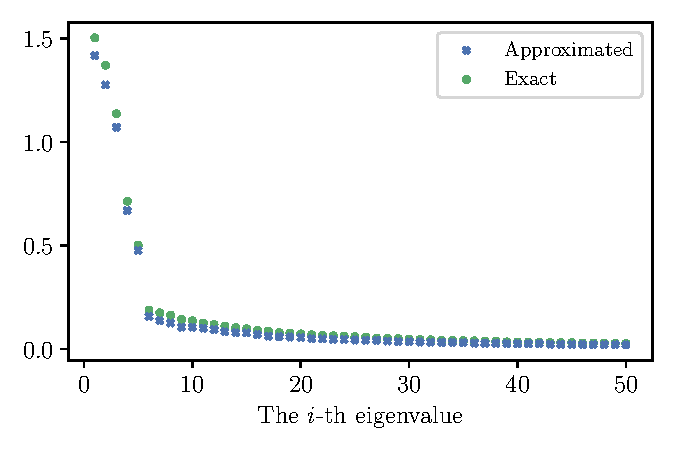
\includegraphics[width=\textwidth]{Appendix_Figures/Full_hessian/newplots/eigenval_fc4_200.pdf}
        \caption{Eigenvalues for F-$200^4$}
    \end{subfigure}%
    \begin{subfigure}[t]{0.5\textwidth}
        \centering
        \captionsetup{justification=centering}
        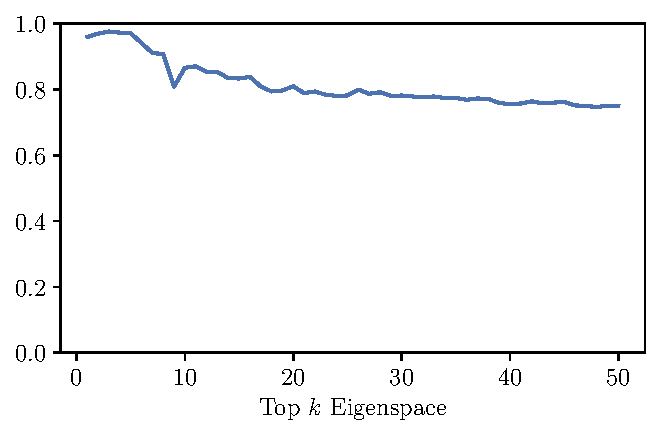
\includegraphics[width=\textwidth]{Appendix_Figures/Full_hessian/newplots/eigenvec_fc4_200.pdf}
        \caption{Eigenspace overlap for F-$200^4$}
    \end{subfigure}\\
    \begin{subfigure}[t]{0.5\textwidth}
        \centering
        \captionsetup{justification=centering}
        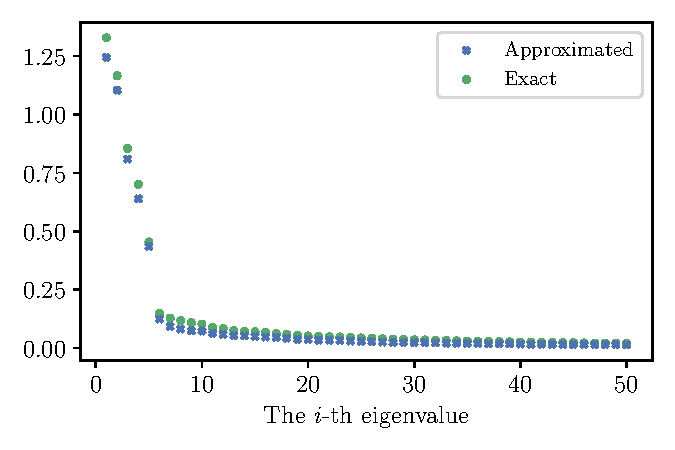
\includegraphics[width=\textwidth]{Appendix_Figures/Full_hessian/newplots/eigenval_fc4_600.pdf}
        \caption{Eigenvalues for F-$600^4$}
    \end{subfigure}%
    \begin{subfigure}[t]{0.5\textwidth}
        \centering
        \captionsetup{justification=centering}
        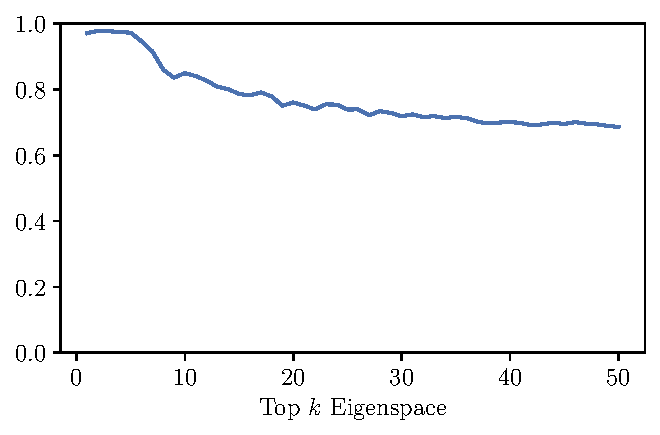
\includegraphics[width=\textwidth]{Appendix_Figures/Full_hessian/newplots/eigenvec_fc4_600.pdf}
        \caption{Eigenspace overlap for F-$600^4$}
    \end{subfigure}\\
    \begin{subfigure}[t]{0.5\textwidth}
        \centering
        \captionsetup{justification=centering}
        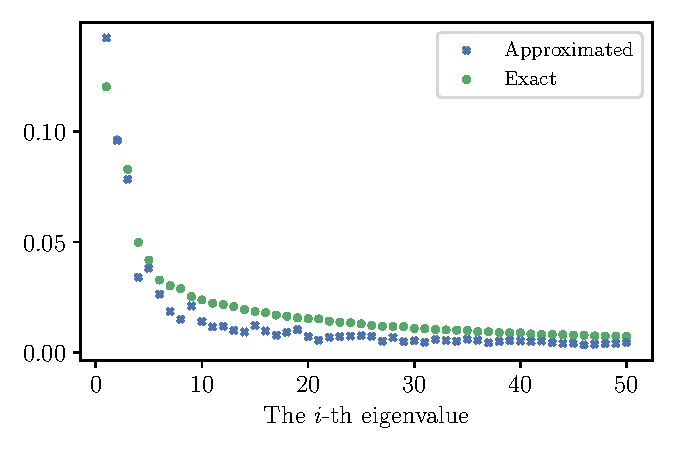
\includegraphics[width=\textwidth]{Appendix_Figures/Full_hessian/newplots/eigenval_fc8_600.pdf}
        \caption{Eigenvalues for F-$600^8$}
    \end{subfigure}%
    \begin{subfigure}[t]{0.5\textwidth}
        \centering
        \captionsetup{justification=centering}
        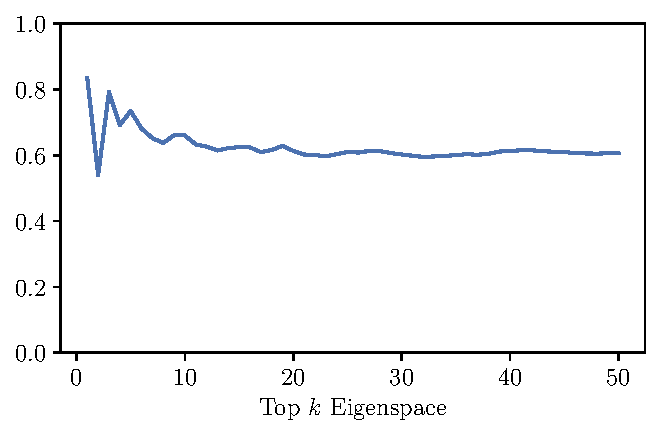
\includegraphics[width=\textwidth]{Appendix_Figures/Full_hessian/newplots/eigenvec_fc8_600.pdf}
        \caption{Eigenspace overlap for F-$600^8$}
    \end{subfigure}\\
    \caption{Top 50 Eigenvalues and Eigenspace approximation for full Hessian}
    \label{fig:Corrfc11}
\end{figure}
% \newpage
% \begin{figure}[h]
%     \centering
%     \vspace{-1em}
%     \subfigure[\small{Eigenvalues for F-$200^2$}]{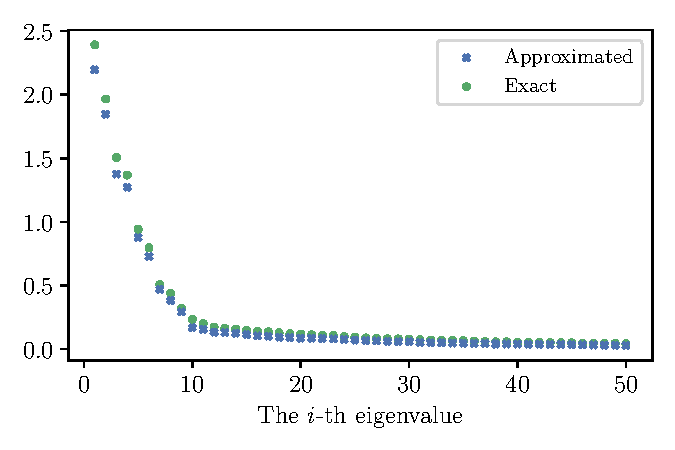
\includegraphics[width=0.42\linewidth]{Appendix_Figures/Full_hessian/newplots/eigenval_fc2_200.pdf}}
%     \subfigure[\small{Eigenspace overlap for F-$200^2$}]{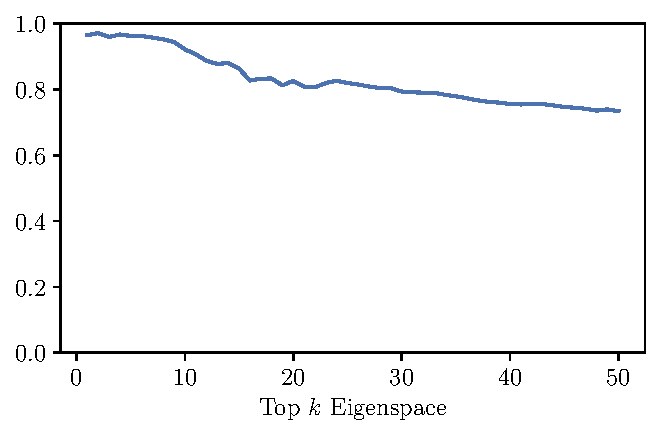
\includegraphics[width=0.42\linewidth]{Appendix_Figures/Full_hessian/newplots/eigenvec_fc2_200.pdf}}\\
%     \subfigure[\small{Eigenvalues for F-$200^4$}]{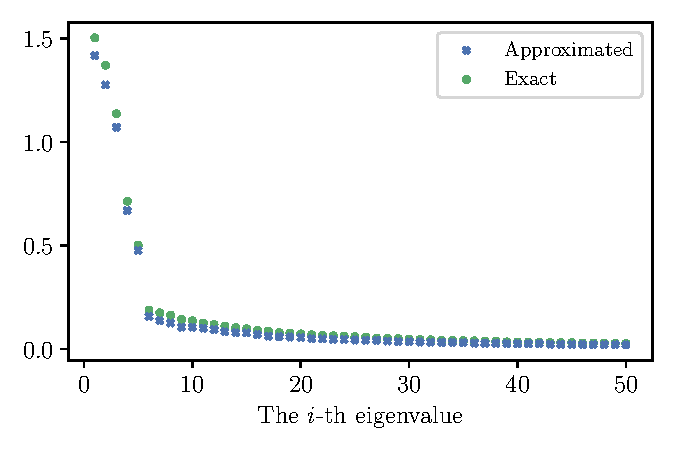
\includegraphics[width=0.42\linewidth]{Appendix_Figures/Full_hessian/newplots/eigenval_fc4_200.pdf}}
%     \subfigure[\small{Eigenspace overlap for F-$200^4$}]{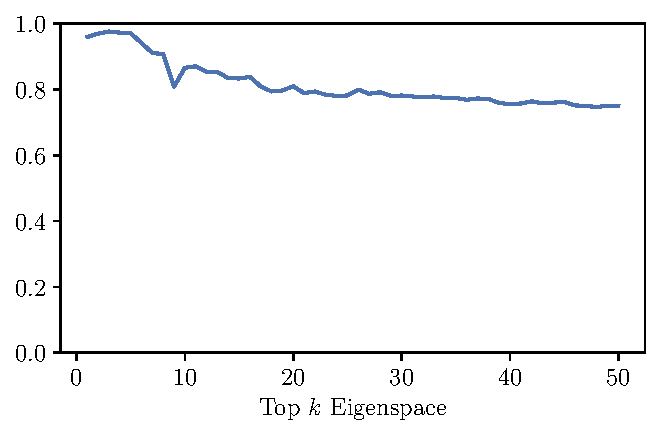
\includegraphics[width=0.42\linewidth]{Appendix_Figures/Full_hessian/newplots/eigenvec_fc4_200.pdf}}\\
%     \subfigure[\small{Eigenvalues for F-$600^4$}]{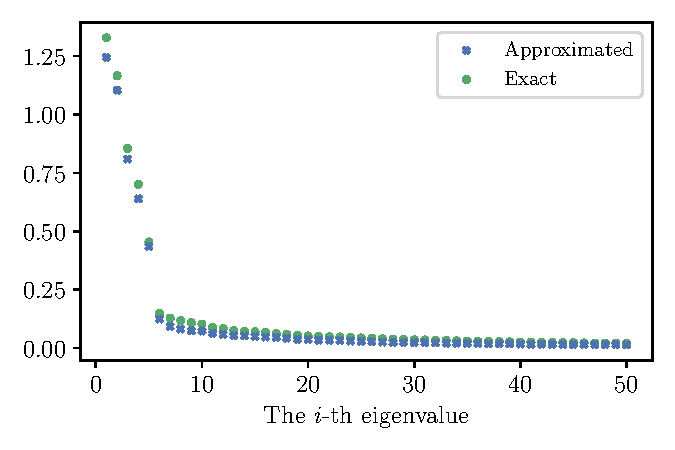
\includegraphics[width=0.42\linewidth]{Appendix_Figures/Full_hessian/newplots/eigenval_fc4_600.pdf}}
%     \subfigure[\small{Eigenspace overlap for F-$600^4$}]{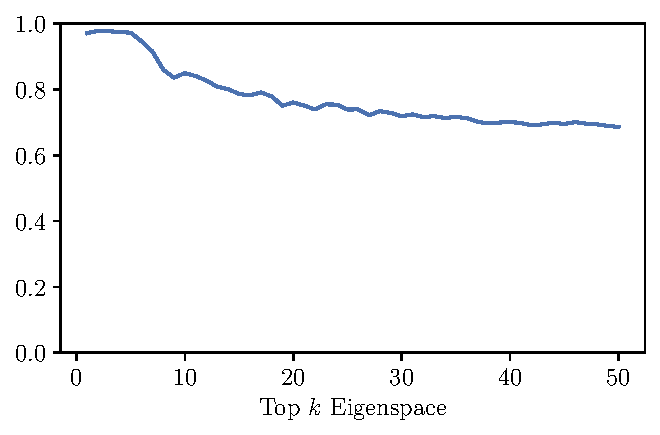
\includegraphics[width=0.42\linewidth]{Appendix_Figures/Full_hessian/newplots/eigenvec_fc4_600.pdf}}\\
%     \subfigure[\small{Eigenvalues for F-$600^8$}]{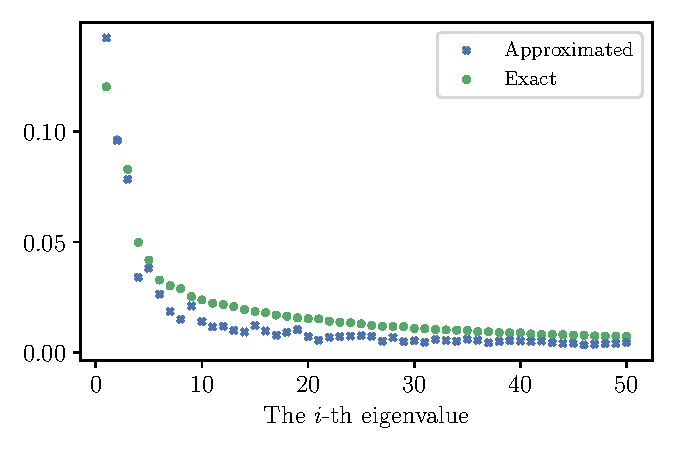
\includegraphics[width=0.42\linewidth]{Appendix_Figures/Full_hessian/newplots/eigenval_fc8_600.pdf}}
%     \subfigure[\small{Eigenspace overlap for F-$600^8$}]{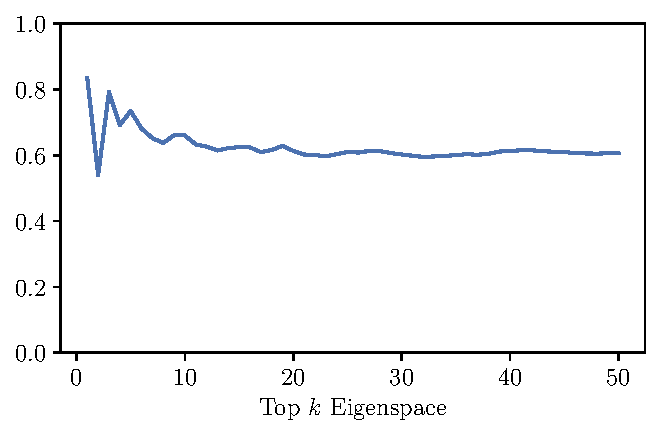
\includegraphics[width=0.42\linewidth]{Appendix_Figures/Full_hessian/newplots/eigenvec_fc8_600.pdf}}\\
%     \caption{Top 50 Eigenvalues and Eigenspace approximation for full Hessian}
%     \label{fig:Corrfc11}
%     \vspace{-1em}
% \end{figure}
\newpage
\section{Computation of Hessian Eigenvalues and Eigenvectors}
\label{sec:appendix_eigencomp}
For Hessian approximated using Kronecker factorization, we compute $\E[\mM]$ and $\E[\vx\vx^T]$ explicitly. Let $\vm$ and $\vv$ be an eigenvector of $\E[\mM]$ and $\E[\vx\vx^T]$ respectively, with corresponding eigenvalues $\lambda_\vm$ and $\lambda_\vv$. Since both matrices are positive semi-definite, $\vm \otimes \vv$ is an eigenvector of $\E[\mM] \otimes \E[\vx\vx^T]$ with eigenvalue $\lambda_\vm\lambda_\vv$. In this way, since $\E[\mM]$ has $m$ eigenvectors and $\E[\vx\vx^T]$ has $n$ eigenvectors, we can approximate all $mn$ eigenvectors for the layer-wise Hessian. All these calculation can be done directly.

However, it is almost prohibitive to calculate the true Hessian explicitly. Thus, we use numerical methods with automatic differentiation \citep{paszke2017automatic} to calculate them. The packages we use is \citet{hessian-eigenthings} and we use the Lanczos method in most of the calculations. We also use package in \citet{yao2019pyhessian} as a reference.

For layer-wise Hessian, we modified the \citet{hessian-eigenthings} package. In particular, the package relies on the calculation of Hessian-vector product $\mH\vv$, where $\vv$ is a vector with the same size as parameter $\theta$. To calculate eigenvalues and eigenvectors for layer-wise Hessian at the $p$-th layer, we cut the $\vv$ into different layers. Then, we only leave the part corresponding to weights of the $p$-th layer and set all other entries to 0. Note that the dimension does not change. We let the new vector be $\vv^{(p)}$ and get the value of $\vu = \mH\vv^{(p)}$ using auto differentiation. Then, we do the same operation to $\vu$ and get $\vu^{(p)}$.
\newpage
\section{Detailed Experiment Setup}
\label{sec:appendix_exp_setup}
\subsection{Datasets}
\label{sec:appendix_exp_dataset}
We conduct experiment on CIFAR-10, CIFAR-100 (MIT) \citep{Krizhevsky09learningmultiple} (\url{https://www.cs.toronto.edu/~kriz/cifar.html}), and MNIST (CC BY-SA 3.0) \citep{lecun1998gradient} (\url{http://yann.lecun.com/exdb/mnist/}). The datasets are downloaded through torchvision \citep{NEURIPS2019_9015} (\url{https://pytorch.org/vision/stable/index.html}). We used their default splitting of training and testing set.

To compare our work on PAC-Bayes bound with the work of \citet{dziugaite2017computing}, we created a custom dataset MNIST-2 by setting the label of images 0-4 to 0 and 5-9 to 1.
We also created random-labeled datasets MNIST-R and CIFAR10-R by randomly labeling the images from the training set of MNIST and CIFAR10.
The dataset information is summarized in \tableref{tab:appendix_dataset}
\begin{table}[h]
\small
  \centering
  \caption{Datasets}
  \vskip 0.1in
    \begin{center}

    \begin{tabular}{lccccc}
    \toprule
    &   \multicolumn{2}{c}{\# Data Points}    &    & &     \\
    Dataset & Train & Test & Input Size & \# Classes & Label \\
    \midrule
    CIFAR10 & 50000 & 10000 & $3\times32\times32$ & 10 & True \\
    CIFAR10-R & 50000 & 10000 & $3\times32\times32$ & 10 & Random \\
    CIFAR100 & 50000 & 10000 & $3\times32\times32$ & 100 & True \\
    MNIST & 60000 & 10000 & $28\times28$ & 10 & True \\
    MNIST-2 & 60000 & 10000 & $28\times28$ & 2 & True \\
    MNIST-R & 60000 & 10000 & $28\times28$ & 10 & Random \\\bottomrule
    \end{tabular}
\end{center}
  \label{tab:appendix_dataset}%
\end{table}%

All the datasets (MNIST, CIFAR-10, and CIFAR-100) we used are publicly available. According to their descriptions on the contents and collection methods, they should not contain any personal information or offensive content. MNIST is a remix of datasets from the National Institute of Standards and Technology (NIST), which obtained consent for collecting the data. However, we also note that CIFAR-10 and CIFAR-100 are subsets of the dataset 80 Million Tiny Image \citep{torralba2007tiny} (\url{http://groups.csail.mit.edu/vision/TinyImages/}), which used automatic collection and includes some offensive images.

\subsection{Network Structures}
\label{appendix_exp_nn}
\paragraph{Fully Connected Network:}
We used several different fully connected networks varying in the number of hidden layers and the number of neurons for each hidden layer. The output of all layers except the last layer are passed into ReLU before feeding into the subsequent layer.  As described in \sectionref{subsec:approx}, we denote a fully connected network with $m$ hidden layers and $n$ neurons each hidden layer by F-$n^m$. For networks without uniform layer width, we denote them by a sequence of numbers (e.g. for a network with three hidden layers, where the first two layers has 200 neurons each and the third has 100 neurons, we denote it as F-$200^2$-$100$). For example, the structure of F-$200^2$ is shown in \tableref{tab:appendix_fc_struct}.

\begin{table}[h]
\small
  \centering
  \caption{Structure of F-$200^2$ on MNIST}
  \vskip 0.1in
    \begin{center}
    \begin{tabular}{rllcc}
    \toprule
    \# & Name & Module & In Shape & Out Shape\\
    \midrule
    1 & & Flatten & (28,28) & 784\\
    2 & fc1 & Linear(784, 200) & 784 & 200\\
    3 & & ReLU & 200 & 200\\
    4 & fc2 & Linear(200, 200) & 200 & 200\\
    5 & & ReLU & 200 & 200\\
    6 & fc3 & Linear(200, 10) & 200 & 10\\
    \multicolumn{5}{c}{\emph{output}}\\\bottomrule
    \end{tabular}%
\end{center}

  \label{tab:appendix_fc_struct}%
\end{table}%

\paragraph{LeNet5:} We adopted the LeNet5 structure proposed by \citet{lecun1998gradient} for MNIST, and slightly modified the input convolutional layers to adapt the input of CIFAR-10 dataset. The standard LeNet5 structure we used in the experiments is shown in \tableref{tab:appendix_lenet_struct}. We further modified the dimension of fc1 and conv2 to create several variants for the experiment in \sectionref{sec:models}. Take the model whose first fully connected layer is adjusted to have 80 neurons as an example, we denote it as LeNet5-(fc1-80).

\begin{table}[h]
\small
  \centering
  \caption{Structure of LeNet5 on CIFAR-10}
  \vskip 0.1in
    \begin{center}
    \begin{tabular}{rllcc}
    \toprule
    \# & Name & Module & In Shape & Out Shape\\\midrule
    1 & conv1 & Conv2D(3, 6, 5, 5) & (3, 32, 32) & (6, 28, 28)\\
    2 & & ReLU & (6, 28, 28) & (6, 28, 28)\\
    3 & maxpool1 & MaxPooling2D(2,2) & (6, 28, 28) & (6, 14, 14)\\
    4 & conv2 & Conv2D(6, 16, 5, 5) & (6, 14, 14) & (16, 10, 10)\\
    5 & & ReLU & (16, 10, 10) & (16, 10, 10)\\
    6 & maxpool2 & MaxPooling2D(2,2) & (16, 10, 10) & (16, 5, 5)\\
    7 & & Flatten & (16, 5, 5) & 400\\
    8 & fc1 & Linear(400, 120) & 400 & 120\\
    9 & & ReLU & 120 & 120\\
    10 & fc2 & Linear(120, 84) & 120 & 84\\
    11 & & ReLU & 84 & 84\\
    12 & fc3 & Linear(84, 10) & 84 & 10\\
    \multicolumn{5}{c}{\emph{output}} \\\bottomrule
    \end{tabular}%
\end{center}
  \label{tab:appendix_lenet_struct}%
\end{table}%

\paragraph{Networks with Batch Normalization:} In \sectionref{sec:appendix_batchnorm} we conducted several experiments regarding the effect of batch normalization on our results. For those experiments, we use the existing structures and add batch normalization layer for each intermediate output after it passes the ReLU module. In order for the Hessian to be well-defined, we fix the running statistics of batch normalization and treat it as a linear layer during inference. We also turn off the learnable parameters $\theta$ and $\beta$ \citep{ioffe2015batch} for simplicity. For network structure X, we denote the variant with batch normalization after all hidden layers X-BN.
For example, the detailed structure LeNet5-BN is shown in \tableref{tab:appendix_lenetBN_struct}.

\begin{table}[h]
\small
  \centering
  \caption{Structure of LeNet5-BN on CIFAR-10}
  \vskip 0.1in
  \begin{center}
    \begin{tabular}{rllcc}
    \toprule
    \# & Name & Module & In Shape & Out Shape\\\midrule
    1 & conv1 & Conv2D(3, 6, 5, 5) & (3, 32, 32) & (6, 28, 28)\\
    2 & & ReLU & (6, 28, 28) & (6, 28, 28)\\
    3 & & BatchNorm2D & (6, 28, 28) & (6, 28, 28)\\
    4 & maxpool1 & MaxPooling2D(2,2) & (6, 28, 28) & (6, 14, 14)\\
    5 & conv2 & Conv2D(6, 16, 5, 5) & (6, 14, 14) & (16, 10, 10)\\
    6 & & ReLU & (16, 10, 10) & (16, 10, 10)\\
    7 & & BatchNorm2D & (16, 10, 10) & (16, 10, 10)\\
    8 & maxpool2 & MaxPooling2D(2,2) & (16, 10, 10) & (16, 5, 5)\\
    9 & & Flatten & (16, 5, 5) & 400\\
    10 & fc1 & Linear(400, 120) & 400 & 120\\
    11 & & ReLU & 120 & 120\\
    12 & & BatchNorm1D & 120 & 120\\
    13 & fc2 & Linear(120, 84) & 120 & 84\\
    14 & & ReLU & 84 & 84\\
    15 & & BatchNorm1D & 84 & 84\\
    16 & fc3 & Linear(84, 10) & 84 & 10\\
    \multicolumn{5}{c}{\emph{output}} \\\bottomrule
    \end{tabular}%
\end{center}
  \label{tab:appendix_lenetBN_struct}%
\end{table}%

\paragraph{Variants of VGG11:} To verify that our results apply to larger networks, we trained a number of variant of VGG11 (originally named VGG-A in the paper, but commonly refered as VGG11) proposed by \citet{simonyan2014very}. For simplicity, we removed the dropout regularization in the original network. To adapt the structure, which is originally designed for the $3\times224\times224$ input of ImageNet, to $3\times32\times32$ input of CIFAR-10.

Since the original VGG11 network is too large for computing the top eigenspace up to hundreds of dimensions, we reduce the number of output channels of each convolution layer in the network to 32, 48, 64, 80, and  200. We denote the small size variants as VGG11-W32, VGG11-W48, VGG11-W64, VGG11-W80, and VGG11-W200 respectively. We use conv1 - conv8 and fc1 to denote the layers of VGG11 where conv1 is closest to the input feature and fc1 is the classification layer.

\paragraph{Variants of ResNet18:} We also trained a number of variant of ResNet18 proposed by \citet{kaiming2015}. As batch normalization will change the low rank structure of the auto correlation matrix and reduce the overlap, we removed all batch normalization operations.
Following the adaptation of ResNet to CIFAR dataset as in \url{https://github.com/kuangliu/pytorch-cifar}, we changed the input size to $3\times32\times32$ and added a 1x1 convolutional layer for each shortcut after the first block.

Similar to VGG11, we reduce the number of output channels of each convolution layer in the network to 48, 64, 80. We denote the small size variants as ResNet18-W48, ResNet18-W64, and ResNet18-W80 respectively.
We use conv1 - conv17 and fc1 to denote the layers of the ResNet18 backbone where conv1 is closest to the input feature and fc1 is the classification layer. For the 1x1 convolutional layers in the shortcut, we denote them by sc-conv1 - sc-conv3. where sc-conv1 is the convolutional layer on the shortcut of the second ResNet block and  sc-conv3 is the convolutional layer on the shortcut of the fourth ResNet block.

\subsection{Training Process and Hyperparameter Configuration}
\label{sec:appendix_exp_train}
For all datasets, we used the default splitting of training and testing set. All models (except explicitly stated otherwise) are trained using batched stochastic gradient descent (SGD) with batch-size 128 and fixed learning rate 0.01 for 1000 epochs. No momentum and weight decay regularization were used. The loss objective converges by the end of training, so we may assume that the final models are at local minima. For generality we also used a training scheme with fixed learning rate at 0.001, and a training scheme with fixed learning rate at 0.01 with momentum of 0.9 and weight-decay factor of 0.0005. Models trained with these settings will be explicitly stated. Otherwise we assume they were trained with the default scheme mentioned above.

Follow the default initialization scheme of PyTorch\citep{NEURIPS2019_9015}, the  weights of linear layers and convolutional layers are initialized using the Xavier method  \citep{glorot2010understanding}, and bias of each layer are initialized to be zero.
\newpage
\section{Additional Empirical Results}
\label{sec:appendix_exp_res}

\subsection{Low Rank Structure of Auto-correlation Matrix \texorpdfstring{$\E[\vx\vx^\T]$}{ExxT}}
\label{sec:appendix_xxT}

We have briefly discussed about the autocorrelation matrix $\E[\vx\vx^\T]$ being approximately rank 1 in \sectionref{sec:xxT} in the main text. In particular, we claimed that the mean of layer input dominate the covariance, that $\E[\vx\vx^\T]\approx \E[\vx]\E[\vx^\T]$. In this section we provide some additional empirical results supporting that claim.

We use two metrics to quantify the quality of this approximation: the squared dot product between normalized $\E[\vx]$ and the first eigenvector of $\E[\vx\vx^\T]$ and the ratio between the first and second eigenvalue of $\E[\vx\vx^\T]$. Intuitively if the first quantity is close to 1 and the second quantity is large, then the approximation is accurate.
Formally, for fully connected layers, define $\hE[\vx]$ as the normalized expectation of the layer input $\vx$, namely ${\E[\vx]}/{\|\E[\vx]\|}$.
For convolutional layers, following the notations in \sectionref{sec:appendix_conv}, define $\hE[\vx]$ as the first left singular vector of $\E[\mX]$ where $\hE[\vx]\in \R^{nK_1K_2}$. Abusing notations for simplicity, we use $\E[\vx\vx^\T]$ to denote the $nK_1K_2\times nK_1K_2$ matrix $\E[\mX\mX^\T]$. In this section we consider the squared dot product between $\hE[\vx]$ and the first eigenvector $\vv_1$ of $\E[\vx\vx^\T]$, namely $(\vv_1^\T\hE[\vx])^2$.

For the spectral ratio, let $\lambda_1$ be the first eigenvalue of $\E[\vx\vx^\T]$ and $\lambda_2$ be the second. We have
\begin{equation}
    \frac{\lambda_1}{\lambda_2} \geq \frac{\|\E[\vx]\E[\vx]^\T\|-\|\mSigma_\vx\| }{\|\mSigma_\vx\|} = \frac{\|\E[\vx]\E[\vx]^\T\|}{\|\mSigma_\vx\|} -1,
\end{equation}
where $\mSigma_\vx$ is the covariance of $\vx$. Thus, the spectral norm of $\E[\vx]\E[\vx]^\T$ divided by that of $\mSigma_\vx$ gives a lower bound to ${\lambda_1}/{\lambda_2}$. In our experiments, we usually have
${\lambda_1}/{\lambda_2} \geq {\|\E[\vx]\E[\vx]^\T\|}/{\|\mSigma_\vx\|}$.

As we can see from \tableref{tab:appendix_xxT_spec_fc} and \tableref{tab:appendix_xxT_spec_conv}, in a variety of settings, $\E[\vx]\E[\vx]^\T$ indeed dominated the autocorrelation matrix $\E[\vx\vx^\T]$ for fully connected layers. Similar phenomenon also holds for convolutional layers in the modern architectures, but the spectral gap are generally smaller compared to that of the fully connected layers.
% The values for F-$200^2$(MNIST) and LeNet5 (CIFAR10) are average of 5 different models. From \cref{tab:appendix_xxT_spec} and \cref{fig:appedix_xxT_lowrank} we can see that the $\mathbb{E}[\vx\vx^\T]$ matrix is close to rank 1 for all the models (without batch normalization) we experiment on, and the principle component is approximately $\hE[x]$ from \cref{tab:appendix_xxT_inner}.
 
\newpage

\begin{table}[h]
\small
  \centering
  \caption{Squared dot product $(\vv_1^\T\hE[\vx])^2$ and spectral ratio $\lambda_1/\lambda_2$ for fully connected layers in a selection of network structures and datasets. We independently trained 5 runs for each instance and compute the mean, minimum, and maximum of the two quantities over all layers (except the first layer which takes the input with mean-zero) in all runs.}
  \vskip 0.1in
    \begin{center}
    \begin{tabular}{llccccccc}
    \toprule
         &                  &              & \multicolumn{3}{c}{$(\vv_1^\T\hE[\vx])^2$} & \multicolumn{3}{c}{$\lambda_1/\lambda_2$} \\
Dataset  & Network          & \# fc & mean        & min         & max         & mean         & min          & max         \\
         \midrule
MNIST    & F-$200^2$        & 2            & 1.000       & 1.000       & 1.000       & 12.29        & 9.65         & 16.16       \\
         & F-$600^2$        & 2            & 0.999       & 0.999       & 0.999       & 12.00        & 11.42        & 13.00       \\
         & F-$600^4$        & 4            & 1.000       & 0.999       & 1.000       & 17.81        & 7.33         & 28.00       \\
         & F-$600^8$        & 8            & 0.991       & 0.965       & 1.000       & 6.63         & 2.28         & 11.15       \\
\midrule
CIFAR10  & F-$600^2$        & 2            & 0.999       & 0.998       & 1.000       & 9.24         & 4.74         & 13.74       \\
         & F-$1500^3$       & 3            & 0.999       & 0.997       & 1.000       & 13.27        & 6.10         & 18.41       \\
         & LeNet5           & 3            & 0.998       & 0.997       & 0.999       & 7.21         & 5.88         & 9.02        \\
         & LeNet5-(fc1-80)  & 3            & 0.998       & 0.996       & 0.999       & 7.80         & 6.77         & 11.01       \\
         & LeNet5-(fc1-100) & 3            & 0.997       & 0.995       & 0.999       & 7.42         & 6.20         & 9.10        \\
         & LeNet5-(fc1-150) & 3            & 0.998       & 0.992       & 0.999       & 7.35         & 5.34         & 9.62        \\
         & VGG11-W32        & 1            & 0.990       & 0.988       & 0.993       & 6.02         & 5.57         & 6.51        \\
         & VGG11-W64        & 1            & 0.996       & 0.993       & 0.999       & 5.87         & 5.32         & 6.26        \\
         & VGG11-W64        & 1            & 0.995       & 0.993       & 0.996       & 6.24         & 5.97         & 6.70        \\
\midrule
CIFAR100 & VGG11-W48        & 1            & 0.999       & 0.999       & 0.999       & 17.861       & 15.456       & 20.491      \\
         & VGG11-W64        & 1            & 0.999       & 0.999       & 1.000       & 19.185       & 18.358       & 20.410      \\
         & VGG11-W80        & 1            & 0.999       & 0.999       & 1.000       & 19.455       & 18.120       & 21.450      \\
         & ResNet18-W48     & 1            & 1.000       & 1.000       & 1.000       & 28.23        & 27.37        & 29.27       \\
         & ResNet18-W64     & 1            & 1.000       & 1.000       & 1.000       & 27.07        & 25.72        & 29.50       \\
         & ResNet18-W80     & 1            & 1.000       & 1.000       & 1.000       & 28.23        & 25.98        & 30.03      \\\bottomrule
\end{tabular}
\end{center}
  \label{tab:appendix_xxT_spec_fc}%
\end{table}
\newpage
\begin{table}[h]
\small
  \centering
  \caption{Squared dot product $(\vv_1^\T\hE[\vx])^2$ and spectral ratio $\lambda_1/\lambda_2$ for convolutional layers in the selection of network structures and datasets in \tableref{tab:appendix_xxT_spec_fc}.}
  \vskip 0.1in
    \begin{center}
    \begin{tabular}{llccccccc}
\toprule
         &                  &         & \multicolumn{3}{c}{$(\vv_1^\T\hE[\vx])^2$} & \multicolumn{3}{c}{$\lambda_1/\lambda_2$} \\
Dataset  & Network          & \# conv & mean        & min         & max         & mean         & min          & max         \\
\midrule
CIFAR10  & LeNet5           & 1       & 0.999       & 0.998       & 0.999       & 15.87        & 11.15        & 27.20       \\
         & LeNet5-(fc1-80)  & 1       & 0.998       & 0.998       & 0.999       & 12.36        & 9.53         & 13.36       \\
         & LeNet5-(fc1-100) & 1       & 0.999       & 0.999       & 0.999       & 19.49        & 16.69        & 21.92       \\
         & LeNet5-(fc1-150) & 1       & 0.999       & 0.998       & 0.999       & 12.86        & 7.65         & 16.34       \\
         & VGG11-W32        & 7       & 0.995       & 0.991       & 0.999       & 5.31         & 2.39         & 9.09        \\
         & VGG11-W64        & 7       & 0.997       & 0.993       & 1.000       & 5.76         & 2.50         & 9.98        \\
         & VGG11-W64        & 7       & 0.998       & 0.995       & 1.000       & 5.81         & 2.53         & 10.62       \\
\midrule
CIFAR100 & VGG11-W48        & 7       & 0.996       & 0.991       & 0.999       & 5.72         & 2.46         & 9.90        \\
         & VGG11-W64        & 7       & 0.995       & 0.991       & 0.999       & 5.66         & 2.50         & 10.79       \\
         & VGG11-W80        & 7       & 0.994       & 0.988       & 0.998       & 5.18         & 2.50         & 8.45        \\
         & ResNet18-W48     & 19      & 0.981       & 0.917       & 0.998       & 3.79         & 1.89         & 7.56        \\
         & ResNet18-W64     & 19      & 0.985       & 0.910       & 0.998       & 3.96         & 1.81         & 7.53        \\
         & ResNet18-W80     & 19      & 0.987       & 0.954       & 0.997       & 4.16         & 2.11         & 7.04        \\ \bottomrule
\end{tabular}
\vspace{-0.15in}
\end{center}
  \label{tab:appendix_xxT_spec_conv}%
\end{table}

% \begin{figure}[ht]
%     \centering
%     \begin{subfigure}[b]{0.27\textwidth}
%         \centering
%         \captionsetup{justification=centering}
%         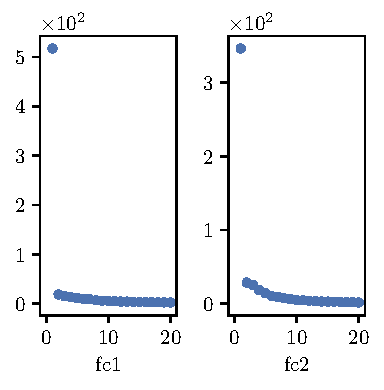
\includegraphics[width=\textwidth]{Figures/Eigenspectrum/xxT/xxT_sigval_d20_MNIST_Exp1_FC2_fixlr0.01R1_E-1_fc1fc2.pdf}

%         \caption{fc1:F-$200^2$ (MNIST)}
%         \label{fig:xxT_sig_lenet_init}%
%     \end{subfigure}
%     \hfill
%     \begin{subfigure}[b]{0.27\textwidth}
%         \centering
%         \captionsetup{justification=centering}
%         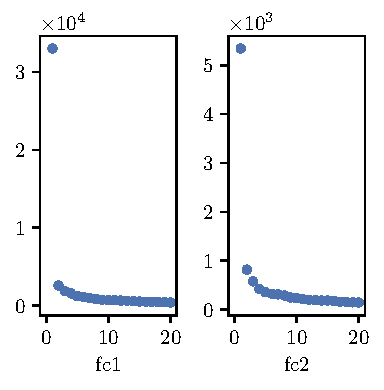
\includegraphics[width=\textwidth]{Figures/Eigenspectrum/xxT/xxT_sigval_d20_CIFAR10_Exp1_LeNet5_fixlr0.01R1_E-1_fc1fc2.pdf}

%         \caption{fc1:LeNet5 (CIFAR10)}
%         \label{fig:xxT_sig_lenet}
%     \end{subfigure}%
%     \hfill
%     \begin{subfigure}[b]{0.27\textwidth}
%         \centering
%         \captionsetup{justification=centering}
%         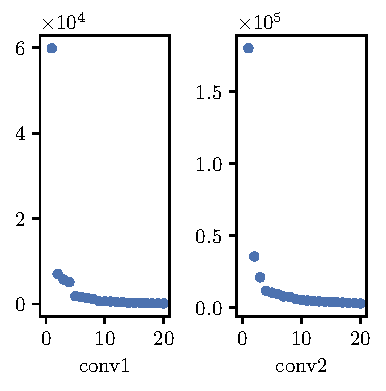
\includegraphics[width=\textwidth]{Figures/Eigenspectrum/xxT/xxTConv_sigval_d20_CIFAR10_Exp1_LeNet5_fixlr0.01_E-1.pdf}

%         \caption{conv1:LeNet5 (CIFAR10)}
%         \label{fig:xxT_sig_lenet_random}
%     \end{subfigure}
%     \captionsetup{justification=centering}

%     \caption{Eigenspectrum of $\E[\vx\vx^\T]$ for different layers in different models. All are close to rank 1.}
%     \label{fig:appedix_xxT_lowrank}
% \end{figure}
\newpage

\subsection{Eigenspace Overlap Between Different Models}
\label{sec:appendix_expres_ovlp}
The non trivial overlap between top eigenspaces of layer-wise Hessians is one of our interesting observations that had been discusses in \sectionref{sec:models}. Here we provide more related empirical results. Some will further verify our claim in \sectionref{sec:models} and some will appear to be challenge that. Both results will be explained discussed more extensively in \sectionref{sec:appendix_explanation}.

\subsubsection{Overlap preserved when varying hyper-parameters:}
We first verify that the overlap also exists for a set of models trained with the different hyper-parameters. Using the LeNet5 (defined in \tableref{tab:appendix_lenet_struct}) as the network structure. We train 6 models using the default training scheme (SGD, lr=0.01, momentum=0), 5 models using a smaller learning rate (SGD, lr=0.001, momentum=0), and 5 models using a combination of optimization tricks (SGD, lr=0.01, momentum=0.9, weight decay=0.0005).
With these 16 models, we compute the pairwise eigenspace overlap of their layer-wise Hessians (120 pairs in total) and plot their average in \figureref{fig:app_overlap_different_hyperparam}. The shade areas in the figure represents the standard deviation. The pattern of overlap is clearly preserved, and the position of the peak roughly agrees with the output dimension $m$, demonstrating that the phenomenon is caused by a common structure instead of similarities in training process.

\begin{figure}[H]
    \centering
    % \vspace{-1em}
    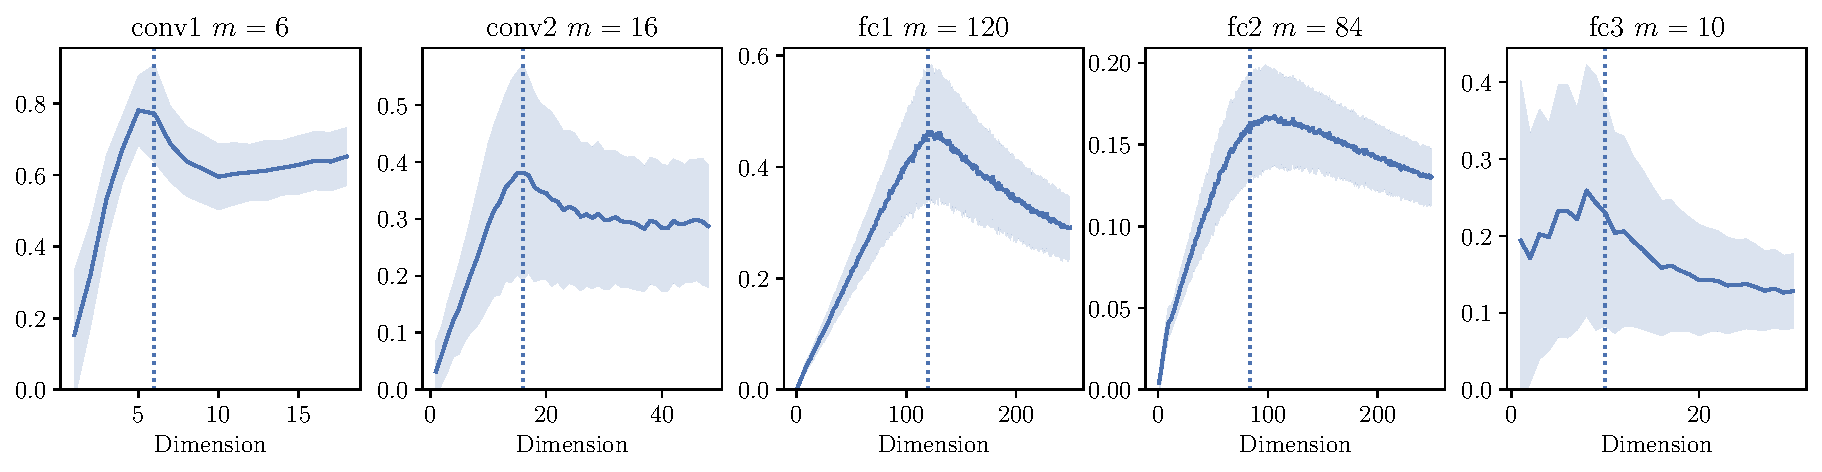
\includegraphics[width=\textwidth]{Appendix_Figures/Overlap_different_models/DimOverlap_CIFAR10_LeNet5_normnew_fixlr0.001_X_LeNet5_normnew_fixlr0.01_X_LeNet5_normnew_fixlr0.01_momentum_appendix_full.pdf}
    \vspace{-1em}
    \caption{Eigenspace overlap of different models of LeNet5 trained with different hyperparameters.}
    \vspace{-1em}
    \label{fig:app_overlap_different_hyperparam}
\end{figure}

Note that for fc3 (the final output layer), we are not observing a linear growth starting from 0 like other layers. This can be explained by the lack of neuron permutation. Related details will be discussed along with the reason for the linear growth pattern for other layers in \sectionref{sec:appendix_model_overlap}.

\subsubsection{Eigenspace overlap for convolutional layers in large models:}
Even though the exact Kroneckor Factorization for layer-wise Hessians is only well-defined for fully connected layers, we also observe similar nontrivial eigenspace overlap for convolutional layers in larger and deeper networks including variants of VGG11 and ResNet18 on datasets CIFAR10 and CIFAR100. Some representative results are shown in \figureref{fig:app_adexp_vgg} and \figureref{fig:app_adexp_resnet}. For each model on each dataset, we independently train 5 models and compute the average pairwise eigenspace overlap. The shade areas represents the standard deviation.
 
For most of the convolutional layers, the eigenspace overlap peaks around the dimension which is equal to the number of output channels of that layer, which is similar to the layers in LeNet5 as in \figureref{fig:app_overlap_different_hyperparam}. The eigenspace overlap of the final fully connected-layer also behaves similar to fc3:LeNet5, which remains around a constant then drops after exceeding the dimension of final output.
However, there are also layers whose overlap does not peak around the output dimensions, (e.g. conv2 of \figureref{fig:app_adexp_vgg}(a) and conv7 of \figureref{fig:app_adexp_resnet}(a)). We will discuss these special cases in the following paragraph.

% \begin{figure}[H]
%     \centering
%     \subfigure[\centering\small{VGG11-W32 (CIFAR10)}]{
%     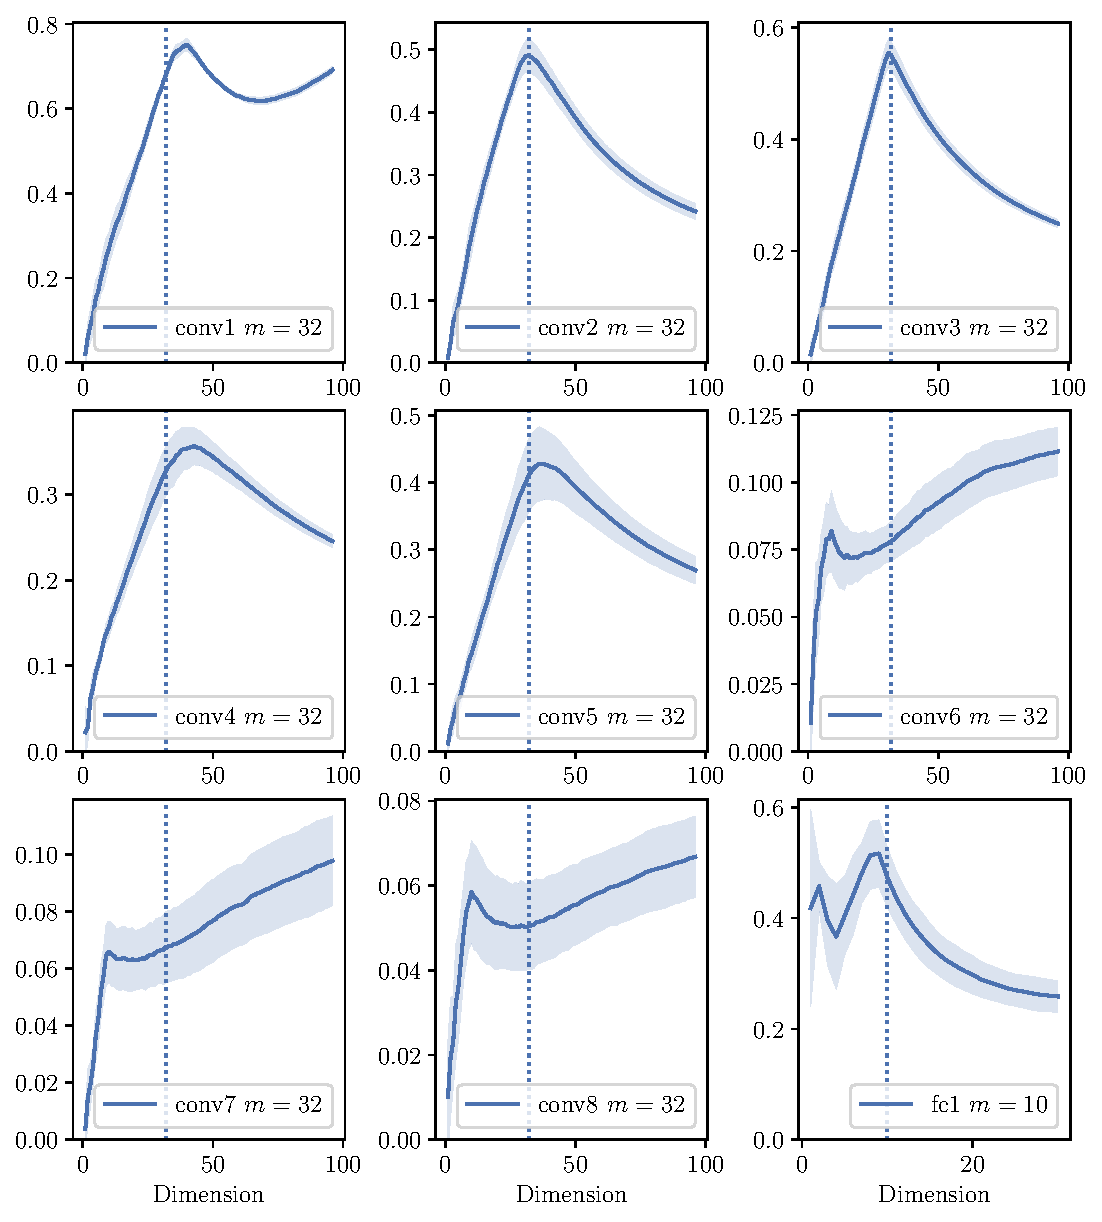
\includegraphics[width=0.48\textwidth]{Appendix_Figures/Overlap_large_model/overlap_raw/DimOverlap_CIFAR10_VGG11W32_fixlr0.01_appendix_vertical_3col.pdf}}
%     \subfigure[\centering\small{VGG11-W200 (CIFAR10)}]{
%     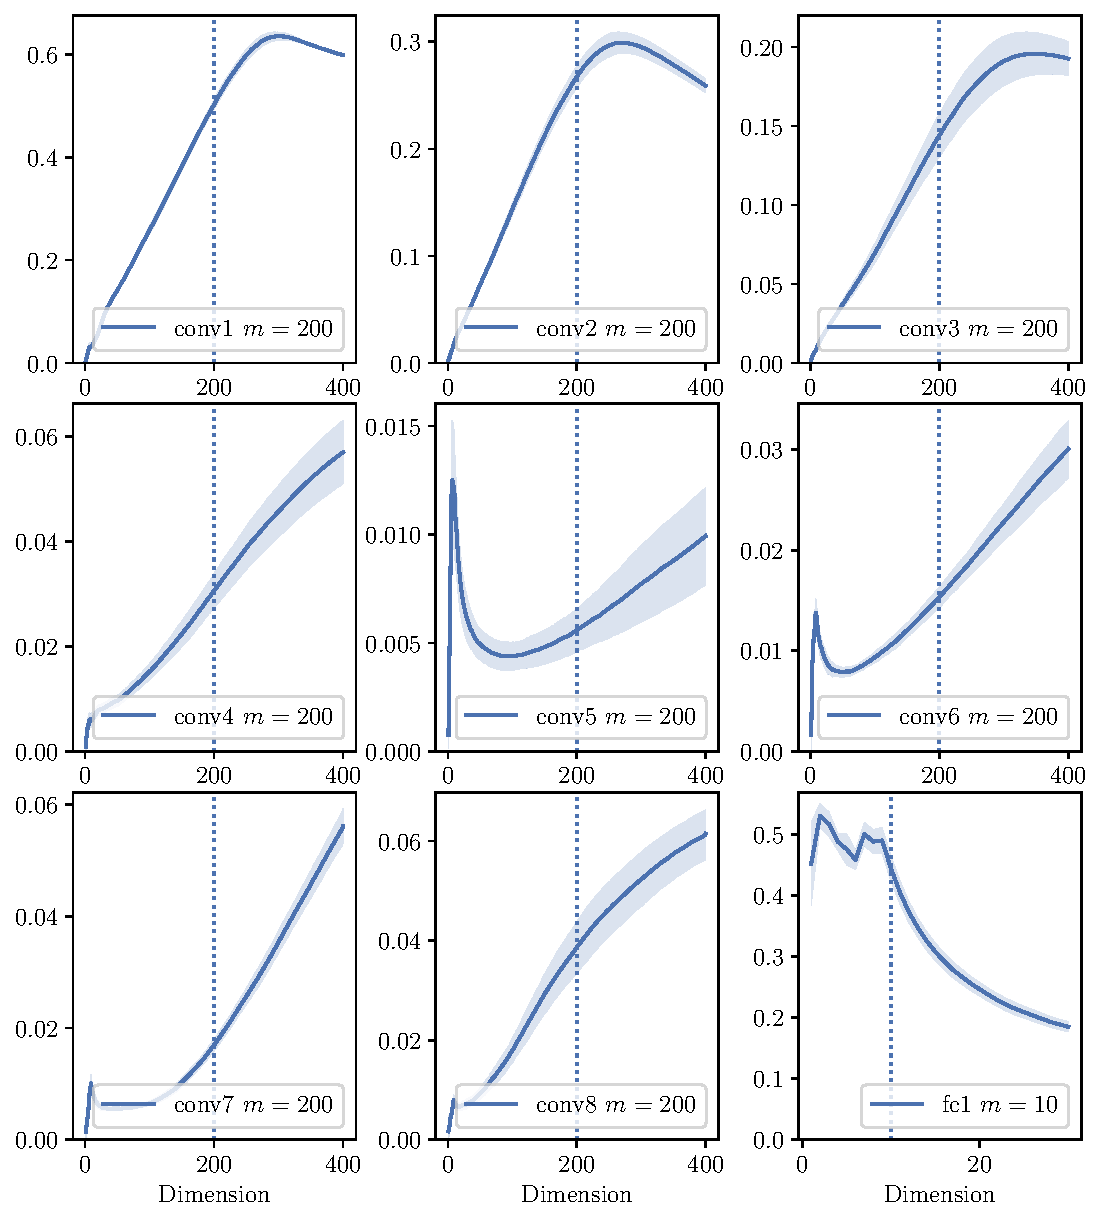
\includegraphics[width=0.48\textwidth]{Appendix_Figures/Overlap_large_model/overlap_raw/DimOverlap_CIFAR10_VGG11W200_fxlr0.01_appendix_vertical_3col.pdf}}\\
%     \subfigure[\centering\small{VGG11-W200 (CIFAR10)}]{
%     \includegraphics[width=0.48\textwidth]{Appendix_Figures/Overlap_large_model/overlap_raw/DimOverlap_CIFAR100_VGG11W48New_nobn_fixlr0.01_appendix_vertical_3col.pdf}}
%     \subfigure[\centering\small{VGG11-W80 (CIFAR100)}]{
%     \includegraphics[width=0.48\textwidth]{Appendix_Figures/Overlap_large_model/overlap_raw/DimOverlap_CIFAR100_VGG11W80New_nobn_fixlr0.01_appendix_vertical_3col.pdf}}
%     \caption{Top Eigenspace overlap for varients of VGG11 on CIFAR10 and CIFAR100.}
%     \label{fig:app_adexp_vgg}
% \end{figure}

\begin{figure}[H]
    \centering
    \begin{subfigure}[b]{0.48\textwidth}
        \centering
        \captionsetup{justification=centering}
        \includegraphics[width=\textwidth]{Appendix_Figures/Overlap_large_model/overlap_raw/DimOverlap_CIFAR10_VGG11W32_fixlr0.01_appendix_vertical_3col.pdf}
        \caption{VGG11-W32 (CIFAR10)}
        \label{fig:app_adexp_cifar10_vgg32}
    \end{subfigure}%
    \ \ \ \ \ \
    \begin{subfigure}[b]{0.48\textwidth}
        \centering
        \captionsetup{justification=centering}
        \includegraphics[width=\textwidth]{Appendix_Figures/Overlap_large_model/overlap_raw/DimOverlap_CIFAR10_VGG11W200_fxlr0.01_appendix_vertical_3col.pdf}
        \caption{VGG11-W200 (CIFAR10)}
        \label{fig:app_adexp_cifar10_vgg200}
    \end{subfigure}
    \\\vspace{0.1in}
    \begin{subfigure}[b]{0.48\textwidth}
        \centering
        \captionsetup{justification=centering}
        \includegraphics[width=\textwidth]{Appendix_Figures/Overlap_large_model/overlap_raw/DimOverlap_CIFAR100_VGG11W48New_nobn_fixlr0.01_appendix_vertical_3col.pdf}
        \caption{VGG11-W48 (CIFAR100)}
        \label{fig:app_adexp_cifar100_vgg48}
    \end{subfigure}%
    \ \ \ \ \ \
    \begin{subfigure}[b]{0.48\textwidth}
        \centering
        \captionsetup{justification=centering}
        \includegraphics[width=\textwidth]{Appendix_Figures/Overlap_large_model/overlap_raw/DimOverlap_CIFAR100_VGG11W80New_nobn_fixlr0.01_appendix_vertical_3col.pdf}
        \caption{VGG11-W80 (CIFAR100)}
        \label{fig:app_adexp_cifar100_vgg80}
    \end{subfigure}
    \captionsetup{justification=centering}
    \caption{Top Eigenspace overlap for varients of VGG11 on CIFAR10 and CIFAR100}
    \label{fig:app_adexp_vgg}
\end{figure}

% \begin{figure}[H]
%     \centering
%     \subfigure[\centering\small{ResNet18-W48 (CIFAR100)}]{
%     \includegraphics[width=0.8\textwidth]{Appendix_Figures/Overlap_large_model/overlap_raw/ResNet/Resnet18W48New_nobn_fixlr0.01_appendix_vertical_7col.pdf}}\\
%     \subfigure[\centering\small{ResNet18-W64 (CIFAR100)}]{
%     \includegraphics[width=0.8\textwidth]{Appendix_Figures/Overlap_large_model/overlap_raw/ResNet/Resnet18W64New_nobn_fixlr0.01_appendix_vertical_7col.pdf}}\\
%     \subfigure[\centering\small{ResNet18-W80 (CIFAR100)}]{
%     \includegraphics[width=0.8\textwidth]{Appendix_Figures/Overlap_large_model/overlap_raw/ResNet/Resnet18W80_nobn_fixlr0.01_appendix_vertical_7col.pdf}}
%     \caption{Top Eigenspace overlap for variants of ResNet18 on CIFAR100}
%     \label{fig:app_adexp_resnet}
% \end{figure}

\begin{figure}[H]
    \centering
    \begin{subfigure}[b]{\textwidth}
        \centering
        \captionsetup{justification=centering}
        \includegraphics[width=\textwidth]{Appendix_Figures/Overlap_large_model/overlap_raw/ResNet/Resnet18W48New_nobn_fixlr0.01_appendix_vertical_7col.pdf}
        \caption{ResNet18-W48 (CIFAR100)}
        \label{fig:app_adexp_cifar100_resnet48}
    \end{subfigure}%
    \\
    \begin{subfigure}[b]{\textwidth}
        \centering
        \captionsetup{justification=centering}
        \includegraphics[width=\textwidth]{Appendix_Figures/Overlap_large_model/overlap_raw/ResNet/Resnet18W64New_nobn_fixlr0.01_appendix_vertical_7col.pdf}
        \caption{ResNet18-W64 (CIFAR100)}
        \label{fig:app_adexp_cifar100_resnet64}
    \end{subfigure}
    \\
    \begin{subfigure}[b]{\textwidth}
        \centering
        \captionsetup{justification=centering}
        \includegraphics[width=\textwidth]{Appendix_Figures/Overlap_large_model/overlap_raw/ResNet/Resnet18W80_nobn_fixlr0.01_appendix_vertical_7col.pdf}
        \caption{ResNet18-W80 (CIFAR100)}
        \label{fig:app_adexp_cifar100_resnet80}
    \end{subfigure}
    \captionsetup{justification=centering}
    \caption{Top Eigenspace overlap for variants of ResNet18 on CIFAR100}
    \label{fig:app_adexp_resnet}
\end{figure}


\subsubsection{Failed cases for eigenspace overlap}
\label{sec:appendix-failed-exp}
As seen in \figureref{fig:app_adexp_vgg} and \figureref{fig:app_adexp_resnet}, there is a small portion of layers, usually closer to the input, whose eigenspace overlap does peak around the output dimensions. These layers can be clustered into the following two general cases.


\paragraph{Early Peak of Low Overlap}
For layers shown in \figureref{fig:app_adexp_failure_early}. The overlap of dominating eigenspaces are significantly lower than the other layers. Also there exists a small peak at very small dimensions.

% \begin{figure}[H]
%     \centering
%     \subfigure[\centering\small{fc2:F-$200^2$\\(MNIST)}]{
%     \includegraphics[width=0.23\textwidth]{Appendix_Figures/Overlap_large_model/FailCases/early/FC2_fixlr0.01_fc2_zoom_stacked.pdf}}
%     \subfigure[\centering\small{conv5:VGG11-W200\\(CIFAR10)}]{
%     \includegraphics[width=0.23\textwidth]{Appendix_Figures/Overlap_large_model/FailCases/early/CIFAR10_VGG11W200_fxlr0.01_conv5_zoom_stacked.pdf}}
%     \subfigure[\centering\small{conv2:VGG11-W80\\(CIFAR100)}]{
%     \includegraphics[width=0.23\textwidth]{Appendix_Figures/Overlap_large_model/FailCases/early/CIFAR100_VGG11W80New_nobn_fixlr0.01_conv2_zoom_stacked.pdf}}
%     \subfigure[\centering\small{conv5:RN18-W64\\(CIFAR100)}]{
%     \includegraphics[width=0.23\textwidth]{Appendix_Figures/Overlap_large_model/FailCases/early/CIFAR100_ResNet18W80_nobn_fixlr0.01_conv5_zoom_stacked.pdf}}
%     \caption{Top eigenspace overlap for layers with an early low peak. Figures in the second row are the zoomed in versions of the figures in the first row. (RN denotes ResNet in (\emph{d}))}
%     \label{fig:app_adexp_failure_early}
% \end{figure}

\begin{figure}[h]
    \centering
    \begin{subfigure}[b]{0.23\textwidth}
        \centering
        \captionsetup{justification=centering}
        \includegraphics[width=\textwidth]{Appendix_Figures/Overlap_large_model/FailCases/early/FC2_fixlr0.01_fc2_zoom_stacked.pdf}
        \caption{fc2:F-$200^2$\\(MNIST)}
        \label{fig:app_adexp_overlap_early_mnistfc2}
    \end{subfigure}
    \begin{subfigure}[b]{0.23\textwidth}
        \centering
        \captionsetup{justification=centering}
        \includegraphics[width=\textwidth]{Appendix_Figures/Overlap_large_model/FailCases/early/CIFAR10_VGG11W200_fxlr0.01_conv5_zoom_stacked.pdf}
        \caption{conv5:VGG11-W200\\(CIFAR10)}
        \label{fig:app_adexp_overlap_early_vgg_cifar10}
    \end{subfigure}
    \begin{subfigure}[b]{0.23\textwidth}
        \centering
        \captionsetup{justification=centering}
        \includegraphics[width=\textwidth]{Appendix_Figures/Overlap_large_model/FailCases/early/CIFAR100_VGG11W80New_nobn_fixlr0.01_conv2_zoom_stacked.pdf}
        \caption{conv2:VGG11-W80\\(CIFAR100)}
        \label{fig:app_adexp_overlap_early_vgg_cifar100}
    \end{subfigure}
    \begin{subfigure}[b]{0.23\textwidth}
        \centering
        \captionsetup{justification=centering}
        \includegraphics[width=\textwidth]{Appendix_Figures/Overlap_large_model/FailCases/early/CIFAR100_Resnet18W80_nobn_fixlr0.01_conv5_zoom_stacked.pdf}
        \caption{conv5:ResNet18-W64\\(CIFAR100)}
        \label{fig:app_adexp_overlap_early_resnet}
    \end{subfigure}
    \captionsetup{justification=centering}
    \caption{Top eigenspace overlap for layers with an early low peak.\\Figures in the second row are the zoomed in versions of the figures in the first row.}
    \label{fig:app_adexp_failure_early}
\end{figure}

\paragraph{Delayed Peak / Peak Doesn't Decline} 
For layers shown in \figureref{fig:app_adexp_failure_late}, the top eigenspaces has a nontrivial overlap, but the peak dimension is larger than predicted output dimension.

% \begin{figure}[H]
%     \centering
%     \subfigure[\centering\small{conv2:VGG11-W200\\(CIFAR10)}]{
%     \includegraphics[width=0.23\textwidth]{Appendix_Figures/Overlap_large_model/FailCases/late/CIFAR10_VGG11W200_fxlr0.01_conv2.pdf}}
%     \subfigure[\centering\small{conv7:VGG11-W48\\(CIFAR100)}]{
%     \includegraphics[width=0.23\textwidth]{Appendix_Figures/Overlap_large_model/FailCases/late/CIFAR100_VGG11W48New_nobn_fixlr0.01_conv7.pdf}}
%     \subfigure[\centering\small{conv7:RN18-W48\\(CIFAR100)}]{
%     \includegraphics[width=0.23\textwidth]{Appendix_Figures/Overlap_large_model/FailCases/late/CIFAR100_Resnet18W48New_nobn_fixlr0.01_conv7.pdf}}
%     \subfigure[\centering\small{conv7:RN18-W64\\(CIFAR100)}]{
%     \includegraphics[width=0.23\textwidth]{Appendix_Figures/Overlap_large_model/FailCases/late/CIFAR100_Resnet18W64New_nobn_fixlr0.01_conv7.pdf}}
%     \caption{Top eigenspace overlap for layers with a delayed peak (RN denotes ResNet).}
%     \label{fig:app_adexp_failure_late}
% \end{figure}

\begin{figure}[h]
    \centering
    \begin{subfigure}[b]{0.23\textwidth}
        \centering
        \captionsetup{justification=centering}
        \includegraphics[width=\textwidth]{Appendix_Figures/Overlap_large_model/FailCases/late/CIFAR10_VGG11W200_fxlr0.01_conv2.pdf}
        \caption{conv2:VGG11-W200\\(CIFAR10)}
        \label{fig:app_adexp_overlap_late_vgg_cifar10}
    \end{subfigure}
    \begin{subfigure}[b]{0.23\textwidth}
        \centering
        \captionsetup{justification=centering}
        \includegraphics[width=\textwidth]{Appendix_Figures/Overlap_large_model/FailCases/late/CIFAR100_VGG11W48New_nobn_fixlr0.01_conv7.pdf}
        \caption{conv7:VGG11-W48\\(CIFAR100)}
        \label{fig:app_adexp_overlap_late_vgg_cifar100}
    \end{subfigure}
    \begin{subfigure}[b]{0.23\textwidth}
        \centering
        \captionsetup{justification=centering}
        \includegraphics[width=\textwidth]{Appendix_Figures/Overlap_large_model/FailCases/late/CIFAR100_Resnet18W48New_nobn_fixlr0.01_conv7.pdf}
        \caption{conv7:VGG11-W48\\(CIFAR100)}
        \label{fig:app_adexp_overlap_late_resnet48}
    \end{subfigure}
    \begin{subfigure}[b]{0.23\textwidth}
        \centering
        \captionsetup{justification=centering}
        \includegraphics[width=\textwidth]{Appendix_Figures/Overlap_large_model/FailCases/late/CIFAR100_Resnet18W64New_nobn_fixlr0.01_conv7.pdf}
        \caption{conv7:ResNet18-W64\\(CIFAR100)}
        \label{fig:app_adexp_overlap_late_resnet}
    \end{subfigure}
    \captionsetup{justification=centering}
    \caption{Top eigenspace overlap for layers with a delayed peak.}
    \label{fig:app_adexp_failure_late}
\end{figure}

However, the existence of such failure cases \emph{does not} undermine the theory of Kronecker factorization approximation. In fact, both appear because the top hessian eigenspace is not completely spanned by $\E[\vx]$,  and can be predicted by computing the auto correlation matrices and the output Hessians. The details will also be elaborated in \sectionref{sec:appendix_model_overlap} with the help of correspondence matrices.

% \paragraph{Overlap may exhibits a early peak for some layers:} For the eigenspace overlap plot of F-$200^2$ (\figureref{fig:app_overlap_fail}), we see that the overlap for fc2 is significantly lower than the other layers, and there exists a small peak near dimension $k=10$. This is because the top hessian eigenspace is not completely spanned by $\E[\vx]$. This phenomenon will also be elaborated in \sectionref{sec:appendix_model_overlap} with the help of correspondence matrices.
% \begin{figure}[h]
%     \centering
%     \includegraphics[width=0.6\textwidth]{Appendix_Figures/Overlap_different_models/DimOverlap_MNIST_FC2_fixlr0.01_appendix_full.pdf}
%     \caption{Eigenspace overlap of different models of F-$200^2$.}
%     \label{fig:app_overlap_fail}

% \end{figure}


\subsection{Eigenvector Correspondence}
\label{sec:app_exp_corr}

In this section, we leverage the idea of eigenvector matricization (\definitionref{def:matricization}) and analyze the validity of the decoupling conjecture using a matrix which we defined as the eigenvector corresponding matrix. First let us recall the definition of eigenvector matricization

\paragraph{\definitionref{def:matricization}} \emph{Consider a layer with input dimension $n$ and output dimension $m$. For an eigenvector $\vh\in\R^{mn}$ of its layer-wise Hessian, the matricized form of $\vh$ is $\Mat(\vh)\in\R^{m\times n}$ where $\Mat(\vh)_{i,j} = \vh_{(i-1)m+j}$.}
\vspace{1em}

Suppose the $i$-th eigenvector for $\E[\vx\vx^\T]$ is $\vv_i$ and the $j$-th eigenvector for $\E[\mM]$ is $\vu_j$. Then the Kronecker product $\E[\mM]\otimes \E[\vx\vx^\T]$ has an eigenvector $\vu_j\otimes \vv_i$. Therefore if the decoupling conjecture is true, one would expect that the top eigenvector of the layer-wise Hessian have a clear correspondence with the top eigenvectors of its two components. Note that $\vu\otimes\vv$ is just the flattened matrix $\vu\vv^\T$.

More concretely, to demonstrate the correspondence between the eigenvectors of the layerwise hessian and the eigenvectors of matrix $\E[\mM]$ and $\E[\vx\vx^\T]$, we introduce ``eigenvector correspondence matrices'' as shown in \figureref{fig:Corr_fc}.
\begin{definition}[Eigenvector Correspondence Matrices]
For layer-wise Hessian matrix $\mH\in\R^{mn\times mn}$ with eigenvectors $\vh_1, \cdots, \vh_{mn}$, and its corresponding auto-correlation matrix $\E[\vx\vx^\T]\in\R^{n\times n}$ with eigenvectors $\vv_1, \cdots, \vv_n$. The correspondence between $\vv_i$ and $\vh_j$ can be defined as \begin{equation}
    \Corr(\vv_i,\vh_j) := \|\Mat(\vh_j)\vv_i\|^2.
\end{equation}
For the output Hessian matrix $\E[\mM]\in\R^{m\times m}$ with eigenvectors $\vu_1, \cdots, \vu_m$, we can likewise define correspondence between $\vv_i$ and $\vh_j$ as
\begin{equation}
    \Corr(\vu_i,\vh_j) := \|\Mat(\vh_j)^\T\vu_i\|^2
\end{equation}
We may then define the eigenvector correspondence matrix between $\mH$ and $\E[\vx\vx^\T]$ as a $n\times mn$ matrix whose $i,j$-th entry is $\Corr(\vv_i,\vh_j)$, and the eigenvector correspondence matrix between $\mH$ and $\E[\mM]$ as a $m\times mn$ matrix whose $i,j$-th entry is $\Corr(\vu_i,\vh_j)$.
\label{def:corr_mat}
\end{definition}

Intuitively, if the $i,j$-th entry of the corresponding matrix is close to 1, then the eigenvector $\vh_j$ is likely to be the Kronecker product of $\vv_i$ (or $\vu_i$) with some vector. Note that if the decoupling conjecture holds absolutely, every eigenvector of the layer-wise Hessian (column of the correspondence matrices) should have a perfect correlation of 1 with exactly one of $\vv_i$ and one of $\vu_i$.
In \figureref{fig:Corr_fc} we can see that the correspondence matrices for the true layer-wise Hessian approximately satisfies this property for top eigenvectors. The similarity between the correspondence patterns for the true and approximated Hessian also verifies the validity of the Kronecker approximation for dominating eigenspace.

% \begin{figure}[th]
%     \centering
%     \subfigure[\small{True Hessian with $\E[\vx\vx^\T].$}]{\includegraphics[width=0.45\textwidth]{Figures/Correspondence/LeNet5_fixlr0.01/xxT_Trueest_real_corr_expand_t200_CIFAR10_Exp1_LeNet5_fixlr0.01R2_E-1_fc1.pdf}}
%     \subfigure[\small{True Hessian with $\E[\mM^\T].$}]{\includegraphics[width=0.45\textwidth]{Figures/Correspondence/LeNet5_fixlr0.01/UTAU_Trueest_real_corr_expand_t200_CIFAR10_Exp1_LeNet5_fixlr0.01R2_E-1_fc1.pdf}\includegraphics[width=0.06\textwidth]{Figures/Misc/colorbar.pdf}}
%     \\
%     \subfigure[\small{Approx Hessian with $\E[\vx\vx^\T].$}]{\includegraphics[width=0.45\textwidth]{Figures/Correspondence/LeNet5_fixlr0.01/xxT_Approxest_real_corr_expand_t200_CIFAR10_Exp1_LeNet5_fixlr0.01R2_E-1_fc1.pdf}}
%     \subfigure[\small{Approx Hessian with $\E[\mM^\T].$}]{\includegraphics[width=0.45\textwidth]{Figures/Correspondence/LeNet5_fixlr0.01/UTAU_Approxest_real_corr_expand_t200_CIFAR10_Exp1_LeNet5_fixlr0.01R2_E-1_fc1.pdf}\includegraphics[width=0.06\textwidth]{Figures/Misc/colorbar.pdf}}
%     \caption{Heatmap of Eigenvector Correspondence Matrices for fc1:LeNet5, which has 120 output neurons. Here we take the top left corner of the eigenvector correspondence matrices. We can see that the top 120 eigenvectors of $\E[\mH]$, roughly corresponds to the top 120 eigenvectors of $\E[\mM]$ (as shown by the diagonal patter of (\emph{b})) and the first eigenvector of $\E[\vx\vx^\T]$ (as shown by the horizontal pattern of (\emph{a})). The similarity between the first row and the second row also shows the validity of the Kronecker approximation}
%     \label{fig:Corr_fc}
%     \vspace{-1em}
%     % \vspace{-4em}
% \end{figure}
In \figureref{fig:Corr_fc}, we show the heatmap of Eigenvector Correspondence Matrices for fc1:LeNet5, which has 120 output neurons. Here we take the top left corner of the eigenvector correspondence matrices. We can see that the top 120 eigenvectors of $\E[\mH]$, roughly corresponds to the top 120 eigenvectors of $\E[\mM]$ (as shown by the diagonal patter of (\emph{b})) and the first eigenvector of $\E[\vx\vx^\T]$ (as shown by the horizontal pattern of (\emph{a})). The similarity between the first row and the second row also shows the validity of the Kronecker approximation.
\label{sec:eigen_corr}
\begin{figure}[H]
    \centering
    \begin{subfigure}[t]{0.46\textwidth}
        \centering
        \captionsetup{justification=centering}
        \includegraphics[width=0.9\textwidth]{Figures/Correspondence/LeNet5_fixlr0.01/xxT_Trueest_real_corr_expand_t200_CIFAR10_Exp1_LeNet5_fixlr0.01R2_E-1_fc1.pdf}
        \caption{True Hessian with $\E[\vx\vx^\T].$}
        \label{fig:Corr_xxT_True_fc}
    \end{subfigure}%
    \begin{subfigure}[t]{0.46\textwidth}
        \centering
        \captionsetup{justification=centering}
        \includegraphics[width=0.9\textwidth]{Figures/Correspondence/LeNet5_fixlr0.01/UTAU_Trueest_real_corr_expand_t200_CIFAR10_Exp1_LeNet5_fixlr0.01R2_E-1_fc1.pdf}
        \caption{True Hessian with $\E[\mM].$}
        \label{fig:Corr_UTAU_True_fc}
    \end{subfigure}%
    \begin{subfigure}[t]{0.065\textwidth}
        \centering
        \includegraphics[width=\textwidth]{Figures/Misc/colorbar.pdf}
    \end{subfigure}
    \bigskip
\begin{subfigure}[t]{0.46\textwidth}
        \centering
        \captionsetup{justification=centering}
        \includegraphics[width=0.9\textwidth]{Figures/Correspondence/LeNet5_fixlr0.01/xxT_Approxest_real_corr_expand_t200_CIFAR10_Exp1_LeNet5_fixlr0.01R2_E-1_fc1.pdf}
        \caption{Approximated Hessian with $\E[\vx\vx^\T].$}
        \label{fig:Corr_xxT_Approx_fc}
    \end{subfigure}%
    \begin{subfigure}[t]{0.46\textwidth}
        \centering
        \captionsetup{justification=centering}
        \includegraphics[width=0.9\textwidth]{Figures/Correspondence/LeNet5_fixlr0.01/UTAU_Approxest_real_corr_expand_t200_CIFAR10_Exp1_LeNet5_fixlr0.01R2_E-1_fc1.pdf}
        \caption{Approximated Hessian with $\E[\vx\vx^\T].$}
        \label{fig:Corr_UTAU_Approx_fc}
    \end{subfigure}%
    \begin{subfigure}[t]{0.065\textwidth}
        \centering
        \includegraphics[width=\textwidth]{Figures/Misc/colorbar.pdf}
    \end{subfigure}
    \captionsetup{justification=centering}
    \caption{Heatmap of Eigenvector Correspondence Matrices for fc1:LeNet5.}
    \label{fig:Corr_fc}
\end{figure}

Here we present the correspondence matrix for fc2, conv1, and conv2 layer of LeNet5. The top eigenvectors for all layers shows a strong correlation with the first eigenvector of $\E[\vx\vx^\T]$ (which is approximately $\hE[\vx]$). For convolutional layers, since the computation of $\mM$ is not exact, the correspondence matrices with $\E[\mM]$ does not exhibit the diagonal pattern. For fc2:LeNet5 as in \figureref{fig:Corrfc22}, the diagonal pattern in (\emph{b}) and the strong correlation with $\E[\vx]$ stops at dimension 9. This fells into one of the ``failed cases'' as described in \sectionref{sec:appendix-failed-exp} case that the small eigenvalues of $\E[\rmM]$ are approaching $0$ faster than $\E[\vx\vx^\T]$. We will discuss this case in more detail in \sectionref{sec:appendix-failure}.


\begin{figure}[H]
    \centering
    \begin{subfigure}[t]{0.5\textwidth}
        \centering
        \captionsetup{justification=centering}
        \includegraphics[width=\textwidth]{Figures/Correspondence/LeNet5_fixlr0.01/xxT_Trueest_real_corr_expand_t200_CIFAR10_Exp1_LeNet5_fixlr0.01R2_E-1_fc1.pdf}
        \caption{Correspondence with $\E[\vx\vx^T].$}
        \label{fig:Corr_xxT_True_fc1}
    \end{subfigure}%
    \begin{subfigure}[t]{0.5\textwidth}
        \centering
        \captionsetup{justification=centering}
        \includegraphics[width=\textwidth]{Figures/Correspondence/LeNet5_fixlr0.01/UTAU_Trueest_real_corr_expand_t200_CIFAR10_Exp1_LeNet5_fixlr0.01R2_E-1_fc1.pdf}
        \caption{Correspondence with $\E[\mM].$}
        \label{fig:Corr_UTAU_True_fc1}
    \end{subfigure}
    \caption{Eigenvector Correspondence for fc1:LeNet5. ($m$=120)}
    \label{fig:Corrfc11}
\end{figure}

\begin{figure}[H]
    \centering
    \begin{subfigure}[t]{0.5\textwidth}
        \centering
        \captionsetup{justification=centering}
        \includegraphics[width=\textwidth]{Figures/Correspondence/LeNet5_fixlr0.01/xxT_Trueest_real_corr_expand_t200_CIFAR10_Exp1_LeNet5_fixlr0.01R2_E-1_fc2.pdf}
        \caption{Correspondence with $\E[\vx\vx^T].$}
        \label{fig:Corr_xxT_True_fc2}
    \end{subfigure}%
    \begin{subfigure}[t]{0.5\textwidth}
        \centering
        \captionsetup{justification=centering}
        \includegraphics[width=\textwidth]{Figures/Correspondence/LeNet5_fixlr0.01/UTAU_Trueest_real_corr_expand_t200_CIFAR10_Exp1_LeNet5_fixlr0.01R2_E-1_fc2.pdf}
        \caption{Correspondence with $\E[\mM].$}
        \label{fig:Corr_UTAU_True_fc2}
    \end{subfigure}
    \caption{Eigenvector Correspondence for fc2:LeNet5. ($m$=84)}
    \label{fig:Corrfc22}
\end{figure}

\begin{figure}[H]
    \centering
    \begin{subfigure}[t]{0.5\textwidth}
        \centering
        \captionsetup{justification=centering}
        \includegraphics[width=\textwidth]{Figures/Correspondence/LeNet5_fixlr0.01/Conv/xxT_Trueest_real_corr_expand_t50_CIFAR10_Exp1_LeNet5_fixlr0.01_E-1_conv1.pdf}
        \caption{Correspondence with $\E[\vx\vx^T].$}
        \label{fig:Corr_xxT_True_conv1}
    \end{subfigure}%
    \begin{subfigure}[t]{0.5\textwidth}
        \centering
        \captionsetup{justification=centering}
        \includegraphics[width=\textwidth]{Figures/Correspondence/LeNet5_fixlr0.01/Conv/UTAU_Trueest_real_corr_expand_t50_CIFAR10_Exp1_LeNet5_fixlr0.01_E-1_conv1.pdf}
        \caption{Correspondence with $\E[\mM].$}
        \label{fig:Corr_UTAU_True_conv1}
    \end{subfigure}
    \caption{Eigenvector Correspondence for conv1:LeNet5. ($m$=6)}
    \label{fig:Corr_conv1}
\end{figure}

\begin{figure}[H]
    \centering
    \begin{subfigure}[t]{0.5\textwidth}
        \centering
        \captionsetup{justification=centering}
        \includegraphics[width=\textwidth]{Figures/Correspondence/LeNet5_fixlr0.01/Conv/xxT_Trueest_real_corr_expand_t50_CIFAR10_Exp1_LeNet5_fixlr0.01_E-1_conv2.pdf}
        \caption{Correspondence with $\E[\vx\vx^T].$}
        \label{fig:Corr_xxT_True_conv2}
    \end{subfigure}%
    \begin{subfigure}[t]{0.5\textwidth}
        \centering
        \captionsetup{justification=centering}
        \includegraphics[width=\textwidth]{Figures/Correspondence/LeNet5_fixlr0.01/Conv/UTAU_Trueest_real_corr_expand_t50_CIFAR10_Exp1_LeNet5_fixlr0.01_E-1_conv2.pdf}
        \caption{Correspondence with $\E[\mM].$}
        \label{fig:Corr_UTAU_True_conv2}
    \end{subfigure}
    \caption{Eigenvector Correspondence for conv2:LeNet5. ($m$=16)}
    \label{fig:Corr_conv2}
\end{figure}


% \begin{figure}[H]
%     \centering
%     \subfigure[\small{Correspondence with $\E[\vx\vx^\T].$}]{\includegraphics[width=0.45\textwidth]{Figures/Correspondence/LeNet5_fixlr0.01/xxT_Trueest_real_corr_expand_t200_CIFAR10_Exp1_LeNet5_fixlr0.01R2_E-1_fc2.pdf}}
%     \subfigure[\small{Correspondence with $\E[\mM].$}]{\includegraphics[width=0.45\textwidth]{Figures/Correspondence/LeNet5_fixlr0.01/UTAU_Trueest_real_corr_expand_t200_CIFAR10_Exp1_LeNet5_fixlr0.01R2_E-1_fc2.pdf}}
%     \caption{Eigenvector Correspondence for fc2:LeNet5. ($m$=84)}
%     \label{fig:Corr_fc2}
%     \vspace{-1em}
%     % \vspace{-4em}
% \end{figure}

% \begin{figure}[H]
%     \centering
%     \subfigure[\small{Correspondence with $\E[\vx\vx^\T].$}]{\includegraphics[width=0.45\textwidth]{Figures/Correspondence/LeNet5_fixlr0.01/Conv/xxT_Trueest_real_corr_expand_t50_CIFAR10_Exp1_LeNet5_fixlr0.01_E-1_conv1.pdf}}
%     \subfigure[\small{Correspondence with $\E[\mM].$}]{\includegraphics[width=0.45\textwidth]{Figures/Correspondence/LeNet5_fixlr0.01/Conv/UTAU_Trueest_real_corr_expand_t50_CIFAR10_Exp1_LeNet5_fixlr0.01_E-1_conv1.pdf}}
%     \caption{Eigenvector Correspondence for conv1:LeNet5. ($m$=6)}
%     \label{fig:Corr_conv1}
%     \vspace{-1em}
%     % \vspace{-4em}
% \end{figure}

% \begin{figure}[H]
%     \centering
%     \subfigure[\small{Correspondence with $\E[\vx\vx^\T].$}]{\includegraphics[width=0.45\textwidth]{Figures/Correspondence/LeNet5_fixlr0.01/Conv/xxT_Trueest_real_corr_expand_t50_CIFAR10_Exp1_LeNet5_fixlr0.01_E-1_conv2.pdf}}
%     \subfigure[\small{Correspondence with $\E[\mM].$}]{\includegraphics[width=0.45\textwidth]{Figures/Correspondence/LeNet5_fixlr0.01/Conv/UTAU_Trueest_real_corr_expand_t50_CIFAR10_Exp1_LeNet5_fixlr0.01_E-1_conv2.pdf}}
%     \caption{Eigenvector Correspondence for conv2:LeNet5. ($m$=16)}
%     \label{fig:Corr_conv2}
%     \vspace{-1em}
%     % \vspace{-4em}
% \end{figure}

For VGG11 we also observe a strong correlation with the first eigenvector of $\E[\vx\vx^\T]$.

% \begin{figure}[H]
%     \centering
%     % \captionsetup{justification=centering}
%     \includegraphics[width=0.8\textwidth]{Appendix_Figures/Correspondance/xxT_Truexxt_corr_expand_t400_CIFAR10_Exp1_VGG11_nobn_fixlr0.01_E-1_features.0.pdf}
%     \caption{Eigenvector Correspondence with $\E[\vx\vx^\T]$ for conv1:VGG11. ($m$=64)}
%     \label{fig:Corr_VGG_conv1}
% \end{figure}

% \begin{figure}[H]
%     \centering
%     % \captionsetup{justification=centering}
%     \includegraphics[width=0.8\textwidth]{Appendix_Figures/Correspondance/xxT_Truexxt_corr_expand_t400_CIFAR10_Exp1_VGG11_nobn_fixlr0.01_E-1_features.3.pdf}
%     \caption{Eigenvector Correspondence with $\E[\vx\vx^\T]$ for conv2:VGG11. ($m$=128)}
%     \label{fig:Corr_VGG_conv2}
% \end{figure}
% \begin{figure}[th]
%     \centering
%     \subfigure[\small{Correspondence with $\E[\vx\vx^\T].$}]{\includegraphics[width=0.45\textwidth]{Figures/Correspondence/LeNet5_fixlr0.01/xxT_Trueest_real_corr_expand_t200_CIFAR10_Exp1_LeNet5_fixlr0.01R2_E-1_fc2.pdf}}
%     \subfigure[\small{Correspondence with $\E[\mM].$}]{\includegraphics[width=0.45\textwidth]{Figures/Correspondence/LeNet5_fixlr0.01/UTAU_Trueest_real_corr_expand_t200_CIFAR10_Exp1_LeNet5_fixlr0.01R2_E-1_fc2.pdf}\includegraphics[width=0.06\textwidth]{Figures/Misc/colorbar.pdf}}
%     \caption{Eigenvector Correspondence for fc2:LeNet5. ($m$=84)}
%     \label{fig:Corr_fc2}
%     \vspace{-1em}
%     % \vspace{-4em}
% \end{figure}


% \begin{figure}[H]
%     \centering
%     \begin{subfigure}[t]{0.5\textwidth}
%         \centering
%         \captionsetup{justification=centering}
%         \includegraphics[width=\textwidth]{Figures/Correspondence/LeNet5_fixlr0.01/xxT_Trueest_real_corr_expand_t200_CIFAR10_Exp1_LeNet5_fixlr0.01R2_E-1_fc1.pdf}
%         \caption{Correspondence with $\E[\vx\vx^\T].$}
%         \label{fig:Corr_xxT_True_fc1}
%     \end{subfigure}%
%     \begin{subfigure}[t]{0.5\textwidth}
%         \centering
%         \captionsetup{justification=centering}
%         \includegraphics[width=\textwidth]{Figures/Correspondence/LeNet5_fixlr0.01/UTAU_Trueest_real_corr_expand_t200_CIFAR10_Exp1_LeNet5_fixlr0.01R2_E-1_fc1.pdf}
%         \caption{Correspondence with $\E[\mM].$}
%         \label{fig:Corr_UTAU_True_fc1}
%     \end{subfigure}
%     \caption{Eigenvector Correspondence for fc1:LeNet5. ($m$=120)}
%     \label{fig:Corrfc11}
% \end{figure}

% \begin{figure}[H]
%     \centering
%     \begin{subfigure}[t]{0.5\textwidth}
%         \centering
%         \captionsetup{justification=centering}
%         \includegraphics[width=\textwidth]{Figures/Correspondence/LeNet5_fixlr0.01/xxT_Trueest_real_corr_expand_t200_CIFAR10_Exp1_LeNet5_fixlr0.01R2_E-1_fc2.pdf}
%         \caption{Correspondence with $\E[\vx\vx^\T].$}
%         \label{fig:Corr_xxT_True_fc2}
%     \end{subfigure}%
%     \begin{subfigure}[t]{0.5\textwidth}
%         \centering
%         \captionsetup{justification=centering}
%         \includegraphics[width=\textwidth]{Figures/Correspondence/LeNet5_fixlr0.01/UTAU_Trueest_real_corr_expand_t200_CIFAR10_Exp1_LeNet5_fixlr0.01R2_E-1_fc2.pdf}
%         \caption{Correspondence with $\E[\mM].$}
%         \label{fig:Corr_UTAU_True_fc2}
%     \end{subfigure}
%     \caption{Eigenvector Correspondence for fc2:LeNet5. ($m$=84)}
%     \label{fig:Corrfc11}
% \end{figure}

% \begin{figure}[H]
%     \centering
%     \begin{subfigure}[t]{0.5\textwidth}
%         \centering
%         \captionsetup{justification=centering}
%         \includegraphics[width=\textwidth]{Figures/Correspondence/LeNet5_fixlr0.01/Conv/xxT_Trueest_real_corr_expand_t50_CIFAR10_Exp1_LeNet5_fixlr0.01_E-1_conv1.pdf}
%         \caption{Correspondence with $\E[\vx\vx^\T].$}
%         \label{fig:Corr_xxT_True_conv1}
%     \end{subfigure}%
%     \begin{subfigure}[t]{0.5\textwidth}
%         \centering
%         \captionsetup{justification=centering}
%         \includegraphics[width=\textwidth]{Figures/Correspondence/LeNet5_fixlr0.01/Conv/UTAU_Trueest_real_corr_expand_t50_CIFAR10_Exp1_LeNet5_fixlr0.01_E-1_conv1.pdf}
%         \caption{Correspondence with $\E[\mM].$}
%         \label{fig:Corr_UTAU_True_conv1}
%     \end{subfigure}
%     \caption{Eigenvector Correspondence for conv1:LeNet5. ($m$=6)}
%     \label{fig:Corr_conv1}
% \end{figure}

% \begin{figure}[H]
%     \centering
%     \begin{subfigure}[t]{0.5\textwidth}
%         \centering
%         \captionsetup{justification=centering}
%         \includegraphics[width=\textwidth]{Figures/Correspondence/LeNet5_fixlr0.01/Conv/xxT_Trueest_real_corr_expand_t50_CIFAR10_Exp1_LeNet5_fixlr0.01_E-1_conv2.pdf}
%         \caption{Correspondence with $\E[\vx\vx^\T].$}
%         \label{fig:Corr_xxT_True_conv2}
%     \end{subfigure}%
%     \begin{subfigure}[t]{0.5\textwidth}
%         \centering
%         \captionsetup{justification=centering}
%         \includegraphics[width=\textwidth]{Figures/Correspondence/LeNet5_fixlr0.01/Conv/UTAU_Trueest_real_corr_expand_t50_CIFAR10_Exp1_LeNet5_fixlr0.01_E-1_conv2.pdf}
%         \caption{Correspondence with $\E[\mM].$}
%         \label{fig:Corr_UTAU_True_conv2}
%     \end{subfigure}
%     \caption{Eigenvector Correspondence for conv2:LeNet5. ($m$=16)}
%     \label{fig:Corr_conv2}
% \end{figure}

% For VGG11 we also observe a strong correlation with the first eigenvector of $\E[\vx\vx^\T]$. However the phenomenon is not as strong as the ones exhibited by LeNet5.

\begin{figure}[H]
    \centering
    \captionsetup{justification=centering}
    \includegraphics[width=0.8\textwidth]{Appendix_Figures/Correspondance/xxT_Truexxt_corr_expand_t400_CIFAR10_Exp1_VGG11_nobn_fixlr0.01_E-1_features.0.pdf}

    \caption{Eigenvector Correspondence with $\E[\vx\vx^\T]$ for conv1:VGG11. ($m$=64)}
    \label{fig:Corr_VGG_conv1}
\end{figure}

\begin{figure}[H]
    \centering
    \captionsetup{justification=centering}
    \includegraphics[width=0.8\textwidth]{Appendix_Figures/Correspondance/xxT_Truexxt_corr_expand_t400_CIFAR10_Exp1_VGG11_nobn_fixlr0.01_E-1_features.3.pdf}

    \caption{Eigenvector Correspondence with $\E[\vx\vx^\T]$ for conv2:VGG11. ($m$=128)}
    \label{fig:Corr_VGG_conv2}
\end{figure}

\begin{figure}[H]
    \centering
    \captionsetup{justification=centering}
    \includegraphics[width=0.8\textwidth]{Appendix_Figures/Correspondance/xxT_Truexxt_corr_expand_t400_CIFAR10_Exp1_VGG11_nobn_fixlr0.01_E-1_features.6.pdf}

    \caption{Eigenvector Correspondence with $\E[\vx\vx^\T]$ for conv3:VGG11. ($m$=256)}
    \label{fig:Corr_VGG_conv2}
\end{figure}

\subsection{Structure of \texorpdfstring{$\E[\vx\vx^\T]$}{ExxT} and \texorpdfstring{$\E[\mM]$}{EM} During Training}
\label{sec:appendix_training_traj}
We observed the pattern of $\E[\vx\vx^\T]$ matrix and $\E[\mM]$ matrix along the training trajectory (\figureref{fig:traj_xxT_lenet5_fc1}, \figureref{fig:traj_UTAU_lenet5_fc1}). It shows that $\E[\vx\vx^\T]$ is always approximately rank 1, and $\E[\mM]$ always have around $c$ large eigenvalues. According to our analysis, since the nontrivial eigenspace overlap is likely to be a consequence of a approximately rank 1 $\E[\vx\vx^\T]$, we would conjecture that the overlap phenomenon is likely to happen on the training trajectory as well.

\begin{figure}[H]
    \centering
    \includegraphics[height=0.2\textheight]{Appendix_Figures/Along_traj/ExxT_val/ExxT_trend_10_CIFAR10_Exp1_LeNet5_fixlr0.01R1_0_1000_fc1.pdf}
    % \captionsetup{justification=centering}
    \caption{Top eigenvalues of $\E[\vx\vx^\T]$ along training trajectory. (fc1:LeNet5)}
    \label{fig:traj_xxT_lenet5_fc1}
\end{figure}

\begin{figure}[H]
    \centering
    \includegraphics[height=0.2\textheight]{Appendix_Figures/Along_traj/UTAU_val/EUTAU_trend_20_CIFAR10_Exp1_LeNet5_fixlr0.01R1_0_1000_fc1.pdf}
    % \captionsetup{justification=centering}
    \caption{Top eigenvalues of $\E[\mM]$ along training trajectory. (fc1:LeNet5)}
    \label{fig:traj_UTAU_lenet5_fc1}
\end{figure}
% % \newpage
% \newpage
% \section{Computation of Hessian Eigenvalues and Eigenvectors}
\label{sec:appendix_eigencomp}
For Hessian approximated using Kronecker factorization, we compute $\E[\mM]$ and $\E[\vx\vx^T]$ explicitly. Let $\vm$ and $\vv$ be an eigenvector of $\E[\mM]$ and $\E[\vx\vx^T]$ respectively, with corresponding eigenvalues $\lambda_\vm$ and $\lambda_\vv$. Since both matrices are positive semi-definite, $\vm \otimes \vv$ is an eigenvector of $\E[\mM] \otimes \E[\vx\vx^T]$ with eigenvalue $\lambda_\vm\lambda_\vv$. In this way, since $\E[\mM]$ has $m$ eigenvectors and $\E[\vx\vx^T]$ has $n$ eigenvectors, we can approximate all $mn$ eigenvectors for the layer-wise Hessian. All these calculation can be done directly.

However, it is almost prohibitive to calculate the true Hessian explicitly. Thus, we use numerical methods with automatic differentiation \citep{paszke2017automatic} to calculate them. The packages we use is \citet{hessian-eigenthings} and we use the Lanczos method in most of the calculations. We also use package in \citet{yao2019pyhessian} as a reference.

For layer-wise Hessian, we modified the \citet{hessian-eigenthings} package. In particular, the package relies on the calculation of Hessian-vector product $\mH\vv$, where $\vv$ is a vector with the same size as parameter $\theta$. To calculate eigenvalues and eigenvectors for layer-wise Hessian at the $p$-th layer, we cut the $\vv$ into different layers. Then, we only leave the part corresponding to weights of the $p$-th layer and set all other entries to 0. Note that the dimension does not change. We let the new vector be $\vv^{(p)}$ and get the value of $\vu = \mH\vv^{(p)}$ using auto differentiation. Then, we do the same operation to $\vu$ and get $\vu^{(p)}$.
% \newpage
\section{Detailed Experiment Setup}
\label{sec:appendix_exp_setup}
\subsection{Datasets}
\label{sec:appendix_exp_dataset}
We conduct experiment on CIFAR-10, CIFAR-100 (MIT) \citep{Krizhevsky09learningmultiple} (\url{https://www.cs.toronto.edu/~kriz/cifar.html}), and MNIST (CC BY-SA 3.0) \citep{lecun1998gradient} (\url{http://yann.lecun.com/exdb/mnist/}). The datasets are downloaded through torchvision \citep{NEURIPS2019_9015} (\url{https://pytorch.org/vision/stable/index.html}). We used their default splitting of training and testing set.

To compare our work on PAC-Bayes bound with the work of \citet{dziugaite2017computing}, we created a custom dataset MNIST-2 by setting the label of images 0-4 to 0 and 5-9 to 1.
We also created random-labeled datasets MNIST-R and CIFAR10-R by randomly labeling the images from the training set of MNIST and CIFAR10.
The dataset information is summarized in \tableref{tab:appendix_dataset}
\begin{table}[h]
\small
  \centering
  \caption{Datasets}
  \vskip 0.1in
    \begin{center}

    \begin{tabular}{lccccc}
    \toprule
    &   \multicolumn{2}{c}{\# Data Points}    &    & &     \\
    Dataset & Train & Test & Input Size & \# Classes & Label \\
    \midrule
    CIFAR10 & 50000 & 10000 & $3\times32\times32$ & 10 & True \\
    CIFAR10-R & 50000 & 10000 & $3\times32\times32$ & 10 & Random \\
    CIFAR100 & 50000 & 10000 & $3\times32\times32$ & 100 & True \\
    MNIST & 60000 & 10000 & $28\times28$ & 10 & True \\
    MNIST-2 & 60000 & 10000 & $28\times28$ & 2 & True \\
    MNIST-R & 60000 & 10000 & $28\times28$ & 10 & Random \\\bottomrule
    \end{tabular}
\end{center}
  \label{tab:appendix_dataset}%
\end{table}%

All the datasets (MNIST, CIFAR-10, and CIFAR-100) we used are publicly available. According to their descriptions on the contents and collection methods, they should not contain any personal information or offensive content. MNIST is a remix of datasets from the National Institute of Standards and Technology (NIST), which obtained consent for collecting the data. However, we also note that CIFAR-10 and CIFAR-100 are subsets of the dataset 80 Million Tiny Image \citep{torralba2007tiny} (\url{http://groups.csail.mit.edu/vision/TinyImages/}), which used automatic collection and includes some offensive images.

\subsection{Network Structures}
\label{appendix_exp_nn}
\paragraph{Fully Connected Network:}
We used several different fully connected networks varying in the number of hidden layers and the number of neurons for each hidden layer. The output of all layers except the last layer are passed into ReLU before feeding into the subsequent layer.  As described in \sectionref{subsec:approx}, we denote a fully connected network with $m$ hidden layers and $n$ neurons each hidden layer by F-$n^m$. For networks without uniform layer width, we denote them by a sequence of numbers (e.g. for a network with three hidden layers, where the first two layers has 200 neurons each and the third has 100 neurons, we denote it as F-$200^2$-$100$). For example, the structure of F-$200^2$ is shown in \tableref{tab:appendix_fc_struct}.

\begin{table}[h]
\small
  \centering
  \caption{Structure of F-$200^2$ on MNIST}
  \vskip 0.1in
    \begin{center}
    \begin{tabular}{rllcc}
    \toprule
    \# & Name & Module & In Shape & Out Shape\\
    \midrule
    1 & & Flatten & (28,28) & 784\\
    2 & fc1 & Linear(784, 200) & 784 & 200\\
    3 & & ReLU & 200 & 200\\
    4 & fc2 & Linear(200, 200) & 200 & 200\\
    5 & & ReLU & 200 & 200\\
    6 & fc3 & Linear(200, 10) & 200 & 10\\
    \multicolumn{5}{c}{\emph{output}}\\\bottomrule
    \end{tabular}%
\end{center}

  \label{tab:appendix_fc_struct}%
\end{table}%

\paragraph{LeNet5:} We adopted the LeNet5 structure proposed by \citet{lecun1998gradient} for MNIST, and slightly modified the input convolutional layers to adapt the input of CIFAR-10 dataset. The standard LeNet5 structure we used in the experiments is shown in \tableref{tab:appendix_lenet_struct}. We further modified the dimension of fc1 and conv2 to create several variants for the experiment in \sectionref{sec:models}. Take the model whose first fully connected layer is adjusted to have 80 neurons as an example, we denote it as LeNet5-(fc1-80).

\begin{table}[h]
\small
  \centering
  \caption{Structure of LeNet5 on CIFAR-10}
  \vskip 0.1in
    \begin{center}
    \begin{tabular}{rllcc}
    \toprule
    \# & Name & Module & In Shape & Out Shape\\\midrule
    1 & conv1 & Conv2D(3, 6, 5, 5) & (3, 32, 32) & (6, 28, 28)\\
    2 & & ReLU & (6, 28, 28) & (6, 28, 28)\\
    3 & maxpool1 & MaxPooling2D(2,2) & (6, 28, 28) & (6, 14, 14)\\
    4 & conv2 & Conv2D(6, 16, 5, 5) & (6, 14, 14) & (16, 10, 10)\\
    5 & & ReLU & (16, 10, 10) & (16, 10, 10)\\
    6 & maxpool2 & MaxPooling2D(2,2) & (16, 10, 10) & (16, 5, 5)\\
    7 & & Flatten & (16, 5, 5) & 400\\
    8 & fc1 & Linear(400, 120) & 400 & 120\\
    9 & & ReLU & 120 & 120\\
    10 & fc2 & Linear(120, 84) & 120 & 84\\
    11 & & ReLU & 84 & 84\\
    12 & fc3 & Linear(84, 10) & 84 & 10\\
    \multicolumn{5}{c}{\emph{output}} \\\bottomrule
    \end{tabular}%
\end{center}
  \label{tab:appendix_lenet_struct}%
\end{table}%

\paragraph{Networks with Batch Normalization:} In \sectionref{sec:appendix_batchnorm} we conducted several experiments regarding the effect of batch normalization on our results. For those experiments, we use the existing structures and add batch normalization layer for each intermediate output after it passes the ReLU module. In order for the Hessian to be well-defined, we fix the running statistics of batch normalization and treat it as a linear layer during inference. We also turn off the learnable parameters $\theta$ and $\beta$ \citep{ioffe2015batch} for simplicity. For network structure X, we denote the variant with batch normalization after all hidden layers X-BN.
For example, the detailed structure LeNet5-BN is shown in \tableref{tab:appendix_lenetBN_struct}.

\begin{table}[h]
\small
  \centering
  \caption{Structure of LeNet5-BN on CIFAR-10}
  \vskip 0.1in
  \begin{center}
    \begin{tabular}{rllcc}
    \toprule
    \# & Name & Module & In Shape & Out Shape\\\midrule
    1 & conv1 & Conv2D(3, 6, 5, 5) & (3, 32, 32) & (6, 28, 28)\\
    2 & & ReLU & (6, 28, 28) & (6, 28, 28)\\
    3 & & BatchNorm2D & (6, 28, 28) & (6, 28, 28)\\
    4 & maxpool1 & MaxPooling2D(2,2) & (6, 28, 28) & (6, 14, 14)\\
    5 & conv2 & Conv2D(6, 16, 5, 5) & (6, 14, 14) & (16, 10, 10)\\
    6 & & ReLU & (16, 10, 10) & (16, 10, 10)\\
    7 & & BatchNorm2D & (16, 10, 10) & (16, 10, 10)\\
    8 & maxpool2 & MaxPooling2D(2,2) & (16, 10, 10) & (16, 5, 5)\\
    9 & & Flatten & (16, 5, 5) & 400\\
    10 & fc1 & Linear(400, 120) & 400 & 120\\
    11 & & ReLU & 120 & 120\\
    12 & & BatchNorm1D & 120 & 120\\
    13 & fc2 & Linear(120, 84) & 120 & 84\\
    14 & & ReLU & 84 & 84\\
    15 & & BatchNorm1D & 84 & 84\\
    16 & fc3 & Linear(84, 10) & 84 & 10\\
    \multicolumn{5}{c}{\emph{output}} \\\bottomrule
    \end{tabular}%
\end{center}
  \label{tab:appendix_lenetBN_struct}%
\end{table}%

\paragraph{Variants of VGG11:} To verify that our results apply to larger networks, we trained a number of variant of VGG11 (originally named VGG-A in the paper, but commonly refered as VGG11) proposed by \citet{simonyan2014very}. For simplicity, we removed the dropout regularization in the original network. To adapt the structure, which is originally designed for the $3\times224\times224$ input of ImageNet, to $3\times32\times32$ input of CIFAR-10.

Since the original VGG11 network is too large for computing the top eigenspace up to hundreds of dimensions, we reduce the number of output channels of each convolution layer in the network to 32, 48, 64, 80, and  200. We denote the small size variants as VGG11-W32, VGG11-W48, VGG11-W64, VGG11-W80, and VGG11-W200 respectively. We use conv1 - conv8 and fc1 to denote the layers of VGG11 where conv1 is closest to the input feature and fc1 is the classification layer.

\paragraph{Variants of ResNet18:} We also trained a number of variant of ResNet18 proposed by \citet{kaiming2015}. As batch normalization will change the low rank structure of the auto correlation matrix and reduce the overlap, we removed all batch normalization operations.
Following the adaptation of ResNet to CIFAR dataset as in \url{https://github.com/kuangliu/pytorch-cifar}, we changed the input size to $3\times32\times32$ and added a 1x1 convolutional layer for each shortcut after the first block.

Similar to VGG11, we reduce the number of output channels of each convolution layer in the network to 48, 64, 80. We denote the small size variants as ResNet18-W48, ResNet18-W64, and ResNet18-W80 respectively.
We use conv1 - conv17 and fc1 to denote the layers of the ResNet18 backbone where conv1 is closest to the input feature and fc1 is the classification layer. For the 1x1 convolutional layers in the shortcut, we denote them by sc-conv1 - sc-conv3. where sc-conv1 is the convolutional layer on the shortcut of the second ResNet block and  sc-conv3 is the convolutional layer on the shortcut of the fourth ResNet block.

\subsection{Training Process and Hyperparameter Configuration}
\label{sec:appendix_exp_train}
For all datasets, we used the default splitting of training and testing set. All models (except explicitly stated otherwise) are trained using batched stochastic gradient descent (SGD) with batch-size 128 and fixed learning rate 0.01 for 1000 epochs. No momentum and weight decay regularization were used. The loss objective converges by the end of training, so we may assume that the final models are at local minima. For generality we also used a training scheme with fixed learning rate at 0.001, and a training scheme with fixed learning rate at 0.01 with momentum of 0.9 and weight-decay factor of 0.0005. Models trained with these settings will be explicitly stated. Otherwise we assume they were trained with the default scheme mentioned above.

Follow the default initialization scheme of PyTorch\citep{NEURIPS2019_9015}, the  weights of linear layers and convolutional layers are initialized using the Xavier method  \citep{glorot2010understanding}, and bias of each layer are initialized to be zero.
% \newpage
\section{Additional Empirical Results}
\label{sec:appendix_exp_res}

\subsection{Low Rank Structure of Auto-correlation Matrix \texorpdfstring{$\E[\vx\vx^\T]$}{ExxT}}
\label{sec:appendix_xxT}

We have briefly discussed about the autocorrelation matrix $\E[\vx\vx^\T]$ being approximately rank 1 in \sectionref{sec:xxT} in the main text. In particular, we claimed that the mean of layer input dominate the covariance, that $\E[\vx\vx^\T]\approx \E[\vx]\E[\vx^\T]$. In this section we provide some additional empirical results supporting that claim.

We use two metrics to quantify the quality of this approximation: the squared dot product between normalized $\E[\vx]$ and the first eigenvector of $\E[\vx\vx^\T]$ and the ratio between the first and second eigenvalue of $\E[\vx\vx^\T]$. Intuitively if the first quantity is close to 1 and the second quantity is large, then the approximation is accurate.
Formally, for fully connected layers, define $\hE[\vx]$ as the normalized expectation of the layer input $\vx$, namely ${\E[\vx]}/{\|\E[\vx]\|}$.
For convolutional layers, following the notations in \sectionref{sec:appendix_conv}, define $\hE[\vx]$ as the first left singular vector of $\E[\mX]$ where $\hE[\vx]\in \R^{nK_1K_2}$. Abusing notations for simplicity, we use $\E[\vx\vx^\T]$ to denote the $nK_1K_2\times nK_1K_2$ matrix $\E[\mX\mX^\T]$. In this section we consider the squared dot product between $\hE[\vx]$ and the first eigenvector $\vv_1$ of $\E[\vx\vx^\T]$, namely $(\vv_1^\T\hE[\vx])^2$.

For the spectral ratio, let $\lambda_1$ be the first eigenvalue of $\E[\vx\vx^\T]$ and $\lambda_2$ be the second. We have
\begin{equation}
    \frac{\lambda_1}{\lambda_2} \geq \frac{\|\E[\vx]\E[\vx]^\T\|-\|\mSigma_\vx\| }{\|\mSigma_\vx\|} = \frac{\|\E[\vx]\E[\vx]^\T\|}{\|\mSigma_\vx\|} -1,
\end{equation}
where $\mSigma_\vx$ is the covariance of $\vx$. Thus, the spectral norm of $\E[\vx]\E[\vx]^\T$ divided by that of $\mSigma_\vx$ gives a lower bound to ${\lambda_1}/{\lambda_2}$. In our experiments, we usually have
${\lambda_1}/{\lambda_2} \geq {\|\E[\vx]\E[\vx]^\T\|}/{\|\mSigma_\vx\|}$.

As we can see from \tableref{tab:appendix_xxT_spec_fc} and \tableref{tab:appendix_xxT_spec_conv}, in a variety of settings, $\E[\vx]\E[\vx]^\T$ indeed dominated the autocorrelation matrix $\E[\vx\vx^\T]$ for fully connected layers. Similar phenomenon also holds for convolutional layers in the modern architectures, but the spectral gap are generally smaller compared to that of the fully connected layers.
% The values for F-$200^2$(MNIST) and LeNet5 (CIFAR10) are average of 5 different models. From \cref{tab:appendix_xxT_spec} and \cref{fig:appedix_xxT_lowrank} we can see that the $\mathbb{E}[\vx\vx^\T]$ matrix is close to rank 1 for all the models (without batch normalization) we experiment on, and the principle component is approximately $\hE[x]$ from \cref{tab:appendix_xxT_inner}.
 
\newpage

\begin{table}[h]
\small
  \centering
  \caption{Squared dot product $(\vv_1^\T\hE[\vx])^2$ and spectral ratio $\lambda_1/\lambda_2$ for fully connected layers in a selection of network structures and datasets. We independently trained 5 runs for each instance and compute the mean, minimum, and maximum of the two quantities over all layers (except the first layer which takes the input with mean-zero) in all runs.}
  \vskip 0.1in
    \begin{center}
    \begin{tabular}{llccccccc}
    \toprule
         &                  &              & \multicolumn{3}{c}{$(\vv_1^\T\hE[\vx])^2$} & \multicolumn{3}{c}{$\lambda_1/\lambda_2$} \\
Dataset  & Network          & \# fc & mean        & min         & max         & mean         & min          & max         \\
         \midrule
MNIST    & F-$200^2$        & 2            & 1.000       & 1.000       & 1.000       & 12.29        & 9.65         & 16.16       \\
         & F-$600^2$        & 2            & 0.999       & 0.999       & 0.999       & 12.00        & 11.42        & 13.00       \\
         & F-$600^4$        & 4            & 1.000       & 0.999       & 1.000       & 17.81        & 7.33         & 28.00       \\
         & F-$600^8$        & 8            & 0.991       & 0.965       & 1.000       & 6.63         & 2.28         & 11.15       \\
\midrule
CIFAR10  & F-$600^2$        & 2            & 0.999       & 0.998       & 1.000       & 9.24         & 4.74         & 13.74       \\
         & F-$1500^3$       & 3            & 0.999       & 0.997       & 1.000       & 13.27        & 6.10         & 18.41       \\
         & LeNet5           & 3            & 0.998       & 0.997       & 0.999       & 7.21         & 5.88         & 9.02        \\
         & LeNet5-(fc1-80)  & 3            & 0.998       & 0.996       & 0.999       & 7.80         & 6.77         & 11.01       \\
         & LeNet5-(fc1-100) & 3            & 0.997       & 0.995       & 0.999       & 7.42         & 6.20         & 9.10        \\
         & LeNet5-(fc1-150) & 3            & 0.998       & 0.992       & 0.999       & 7.35         & 5.34         & 9.62        \\
         & VGG11-W32        & 1            & 0.990       & 0.988       & 0.993       & 6.02         & 5.57         & 6.51        \\
         & VGG11-W64        & 1            & 0.996       & 0.993       & 0.999       & 5.87         & 5.32         & 6.26        \\
         & VGG11-W64        & 1            & 0.995       & 0.993       & 0.996       & 6.24         & 5.97         & 6.70        \\
\midrule
CIFAR100 & VGG11-W48        & 1            & 0.999       & 0.999       & 0.999       & 17.861       & 15.456       & 20.491      \\
         & VGG11-W64        & 1            & 0.999       & 0.999       & 1.000       & 19.185       & 18.358       & 20.410      \\
         & VGG11-W80        & 1            & 0.999       & 0.999       & 1.000       & 19.455       & 18.120       & 21.450      \\
         & ResNet18-W48     & 1            & 1.000       & 1.000       & 1.000       & 28.23        & 27.37        & 29.27       \\
         & ResNet18-W64     & 1            & 1.000       & 1.000       & 1.000       & 27.07        & 25.72        & 29.50       \\
         & ResNet18-W80     & 1            & 1.000       & 1.000       & 1.000       & 28.23        & 25.98        & 30.03      \\\bottomrule
\end{tabular}
\end{center}
  \label{tab:appendix_xxT_spec_fc}%
\end{table}
\newpage
\begin{table}[h]
\small
  \centering
  \caption{Squared dot product $(\vv_1^\T\hE[\vx])^2$ and spectral ratio $\lambda_1/\lambda_2$ for convolutional layers in the selection of network structures and datasets in \tableref{tab:appendix_xxT_spec_fc}.}
  \vskip 0.1in
    \begin{center}
    \begin{tabular}{llccccccc}
\toprule
         &                  &         & \multicolumn{3}{c}{$(\vv_1^\T\hE[\vx])^2$} & \multicolumn{3}{c}{$\lambda_1/\lambda_2$} \\
Dataset  & Network          & \# conv & mean        & min         & max         & mean         & min          & max         \\
\midrule
CIFAR10  & LeNet5           & 1       & 0.999       & 0.998       & 0.999       & 15.87        & 11.15        & 27.20       \\
         & LeNet5-(fc1-80)  & 1       & 0.998       & 0.998       & 0.999       & 12.36        & 9.53         & 13.36       \\
         & LeNet5-(fc1-100) & 1       & 0.999       & 0.999       & 0.999       & 19.49        & 16.69        & 21.92       \\
         & LeNet5-(fc1-150) & 1       & 0.999       & 0.998       & 0.999       & 12.86        & 7.65         & 16.34       \\
         & VGG11-W32        & 7       & 0.995       & 0.991       & 0.999       & 5.31         & 2.39         & 9.09        \\
         & VGG11-W64        & 7       & 0.997       & 0.993       & 1.000       & 5.76         & 2.50         & 9.98        \\
         & VGG11-W64        & 7       & 0.998       & 0.995       & 1.000       & 5.81         & 2.53         & 10.62       \\
\midrule
CIFAR100 & VGG11-W48        & 7       & 0.996       & 0.991       & 0.999       & 5.72         & 2.46         & 9.90        \\
         & VGG11-W64        & 7       & 0.995       & 0.991       & 0.999       & 5.66         & 2.50         & 10.79       \\
         & VGG11-W80        & 7       & 0.994       & 0.988       & 0.998       & 5.18         & 2.50         & 8.45        \\
         & ResNet18-W48     & 19      & 0.981       & 0.917       & 0.998       & 3.79         & 1.89         & 7.56        \\
         & ResNet18-W64     & 19      & 0.985       & 0.910       & 0.998       & 3.96         & 1.81         & 7.53        \\
         & ResNet18-W80     & 19      & 0.987       & 0.954       & 0.997       & 4.16         & 2.11         & 7.04        \\ \bottomrule
\end{tabular}
\vspace{-0.15in}
\end{center}
  \label{tab:appendix_xxT_spec_conv}%
\end{table}

% \begin{figure}[ht]
%     \centering
%     \begin{subfigure}[b]{0.27\textwidth}
%         \centering
%         \captionsetup{justification=centering}
%         \includegraphics[width=\textwidth]{Figures/Eigenspectrum/xxT/xxT_sigval_d20_MNIST_Exp1_FC2_fixlr0.01R1_E-1_fc1fc2.pdf}

%         \caption{fc1:F-$200^2$ (MNIST)}
%         \label{fig:xxT_sig_lenet_init}%
%     \end{subfigure}
%     \hfill
%     \begin{subfigure}[b]{0.27\textwidth}
%         \centering
%         \captionsetup{justification=centering}
%         \includegraphics[width=\textwidth]{Figures/Eigenspectrum/xxT/xxT_sigval_d20_CIFAR10_Exp1_LeNet5_fixlr0.01R1_E-1_fc1fc2.pdf}

%         \caption{fc1:LeNet5 (CIFAR10)}
%         \label{fig:xxT_sig_lenet}
%     \end{subfigure}%
%     \hfill
%     \begin{subfigure}[b]{0.27\textwidth}
%         \centering
%         \captionsetup{justification=centering}
%         \includegraphics[width=\textwidth]{Figures/Eigenspectrum/xxT/xxTConv_sigval_d20_CIFAR10_Exp1_LeNet5_fixlr0.01_E-1.pdf}

%         \caption{conv1:LeNet5 (CIFAR10)}
%         \label{fig:xxT_sig_lenet_random}
%     \end{subfigure}
%     \captionsetup{justification=centering}

%     \caption{Eigenspectrum of $\E[\vx\vx^\T]$ for different layers in different models. All are close to rank 1.}
%     \label{fig:appedix_xxT_lowrank}
% \end{figure}
\newpage

\subsection{Eigenspace Overlap Between Different Models}
\label{sec:appendix_expres_ovlp}
The non trivial overlap between top eigenspaces of layer-wise Hessians is one of our interesting observations that had been discusses in \sectionref{sec:models}. Here we provide more related empirical results. Some will further verify our claim in \sectionref{sec:models} and some will appear to be challenge that. Both results will be explained discussed more extensively in \sectionref{sec:appendix_explanation}.

\subsubsection{Overlap preserved when varying hyper-parameters:}
We first verify that the overlap also exists for a set of models trained with the different hyper-parameters. Using the LeNet5 (defined in \tableref{tab:appendix_lenet_struct}) as the network structure. We train 6 models using the default training scheme (SGD, lr=0.01, momentum=0), 5 models using a smaller learning rate (SGD, lr=0.001, momentum=0), and 5 models using a combination of optimization tricks (SGD, lr=0.01, momentum=0.9, weight decay=0.0005).
With these 16 models, we compute the pairwise eigenspace overlap of their layer-wise Hessians (120 pairs in total) and plot their average in \figureref{fig:app_overlap_different_hyperparam}. The shade areas in the figure represents the standard deviation. The pattern of overlap is clearly preserved, and the position of the peak roughly agrees with the output dimension $m$, demonstrating that the phenomenon is caused by a common structure instead of similarities in training process.

\begin{figure}[H]
    \centering
    % \vspace{-1em}
    \includegraphics[width=\textwidth]{Appendix_Figures/Overlap_different_models/DimOverlap_CIFAR10_LeNet5_normnew_fixlr0.001_X_LeNet5_normnew_fixlr0.01_X_LeNet5_normnew_fixlr0.01_momentum_appendix_full.pdf}
    \vspace{-1em}
    \caption{Eigenspace overlap of different models of LeNet5 trained with different hyperparameters.}
    \vspace{-1em}
    \label{fig:app_overlap_different_hyperparam}
\end{figure}

Note that for fc3 (the final output layer), we are not observing a linear growth starting from 0 like other layers. This can be explained by the lack of neuron permutation. Related details will be discussed along with the reason for the linear growth pattern for other layers in \sectionref{sec:appendix_model_overlap}.

\subsubsection{Eigenspace overlap for convolutional layers in large models:}
Even though the exact Kroneckor Factorization for layer-wise Hessians is only well-defined for fully connected layers, we also observe similar nontrivial eigenspace overlap for convolutional layers in larger and deeper networks including variants of VGG11 and ResNet18 on datasets CIFAR10 and CIFAR100. Some representative results are shown in \figureref{fig:app_adexp_vgg} and \figureref{fig:app_adexp_resnet}. For each model on each dataset, we independently train 5 models and compute the average pairwise eigenspace overlap. The shade areas represents the standard deviation.
 
For most of the convolutional layers, the eigenspace overlap peaks around the dimension which is equal to the number of output channels of that layer, which is similar to the layers in LeNet5 as in \figureref{fig:app_overlap_different_hyperparam}. The eigenspace overlap of the final fully connected-layer also behaves similar to fc3:LeNet5, which remains around a constant then drops after exceeding the dimension of final output.
However, there are also layers whose overlap does not peak around the output dimensions, (e.g. conv2 of \figureref{fig:app_adexp_vgg}(a) and conv7 of \figureref{fig:app_adexp_resnet}(a)). We will discuss these special cases in the following paragraph.

% \begin{figure}[H]
%     \centering
%     \subfigure[\centering\small{VGG11-W32 (CIFAR10)}]{
%     \includegraphics[width=0.48\textwidth]{Appendix_Figures/Overlap_large_model/overlap_raw/DimOverlap_CIFAR10_VGG11W32_fixlr0.01_appendix_vertical_3col.pdf}}
%     \subfigure[\centering\small{VGG11-W200 (CIFAR10)}]{
%     \includegraphics[width=0.48\textwidth]{Appendix_Figures/Overlap_large_model/overlap_raw/DimOverlap_CIFAR10_VGG11W200_fxlr0.01_appendix_vertical_3col.pdf}}\\
%     \subfigure[\centering\small{VGG11-W200 (CIFAR10)}]{
%     \includegraphics[width=0.48\textwidth]{Appendix_Figures/Overlap_large_model/overlap_raw/DimOverlap_CIFAR100_VGG11W48New_nobn_fixlr0.01_appendix_vertical_3col.pdf}}
%     \subfigure[\centering\small{VGG11-W80 (CIFAR100)}]{
%     \includegraphics[width=0.48\textwidth]{Appendix_Figures/Overlap_large_model/overlap_raw/DimOverlap_CIFAR100_VGG11W80New_nobn_fixlr0.01_appendix_vertical_3col.pdf}}
%     \caption{Top Eigenspace overlap for varients of VGG11 on CIFAR10 and CIFAR100.}
%     \label{fig:app_adexp_vgg}
% \end{figure}

\begin{figure}[H]
    \centering
    \begin{subfigure}[b]{0.48\textwidth}
        \centering
        \captionsetup{justification=centering}
        \includegraphics[width=\textwidth]{Appendix_Figures/Overlap_large_model/overlap_raw/DimOverlap_CIFAR10_VGG11W32_fixlr0.01_appendix_vertical_3col.pdf}
        \caption{VGG11-W32 (CIFAR10)}
        \label{fig:app_adexp_cifar10_vgg32}
    \end{subfigure}%
    \ \ \ \ \ \
    \begin{subfigure}[b]{0.48\textwidth}
        \centering
        \captionsetup{justification=centering}
        \includegraphics[width=\textwidth]{Appendix_Figures/Overlap_large_model/overlap_raw/DimOverlap_CIFAR10_VGG11W200_fxlr0.01_appendix_vertical_3col.pdf}
        \caption{VGG11-W200 (CIFAR10)}
        \label{fig:app_adexp_cifar10_vgg200}
    \end{subfigure}
    \\\vspace{0.1in}
    \begin{subfigure}[b]{0.48\textwidth}
        \centering
        \captionsetup{justification=centering}
        \includegraphics[width=\textwidth]{Appendix_Figures/Overlap_large_model/overlap_raw/DimOverlap_CIFAR100_VGG11W48New_nobn_fixlr0.01_appendix_vertical_3col.pdf}
        \caption{VGG11-W48 (CIFAR100)}
        \label{fig:app_adexp_cifar100_vgg48}
    \end{subfigure}%
    \ \ \ \ \ \
    \begin{subfigure}[b]{0.48\textwidth}
        \centering
        \captionsetup{justification=centering}
        \includegraphics[width=\textwidth]{Appendix_Figures/Overlap_large_model/overlap_raw/DimOverlap_CIFAR100_VGG11W80New_nobn_fixlr0.01_appendix_vertical_3col.pdf}
        \caption{VGG11-W80 (CIFAR100)}
        \label{fig:app_adexp_cifar100_vgg80}
    \end{subfigure}
    \captionsetup{justification=centering}
    \caption{Top Eigenspace overlap for varients of VGG11 on CIFAR10 and CIFAR100}
    \label{fig:app_adexp_vgg}
\end{figure}

% \begin{figure}[H]
%     \centering
%     \subfigure[\centering\small{ResNet18-W48 (CIFAR100)}]{
%     \includegraphics[width=0.8\textwidth]{Appendix_Figures/Overlap_large_model/overlap_raw/ResNet/Resnet18W48New_nobn_fixlr0.01_appendix_vertical_7col.pdf}}\\
%     \subfigure[\centering\small{ResNet18-W64 (CIFAR100)}]{
%     \includegraphics[width=0.8\textwidth]{Appendix_Figures/Overlap_large_model/overlap_raw/ResNet/Resnet18W64New_nobn_fixlr0.01_appendix_vertical_7col.pdf}}\\
%     \subfigure[\centering\small{ResNet18-W80 (CIFAR100)}]{
%     \includegraphics[width=0.8\textwidth]{Appendix_Figures/Overlap_large_model/overlap_raw/ResNet/Resnet18W80_nobn_fixlr0.01_appendix_vertical_7col.pdf}}
%     \caption{Top Eigenspace overlap for variants of ResNet18 on CIFAR100}
%     \label{fig:app_adexp_resnet}
% \end{figure}

\begin{figure}[H]
    \centering
    \begin{subfigure}[b]{\textwidth}
        \centering
        \captionsetup{justification=centering}
        \includegraphics[width=\textwidth]{Appendix_Figures/Overlap_large_model/overlap_raw/ResNet/Resnet18W48New_nobn_fixlr0.01_appendix_vertical_7col.pdf}
        \caption{ResNet18-W48 (CIFAR100)}
        \label{fig:app_adexp_cifar100_resnet48}
    \end{subfigure}%
    \\
    \begin{subfigure}[b]{\textwidth}
        \centering
        \captionsetup{justification=centering}
        \includegraphics[width=\textwidth]{Appendix_Figures/Overlap_large_model/overlap_raw/ResNet/Resnet18W64New_nobn_fixlr0.01_appendix_vertical_7col.pdf}
        \caption{ResNet18-W64 (CIFAR100)}
        \label{fig:app_adexp_cifar100_resnet64}
    \end{subfigure}
    \\
    \begin{subfigure}[b]{\textwidth}
        \centering
        \captionsetup{justification=centering}
        \includegraphics[width=\textwidth]{Appendix_Figures/Overlap_large_model/overlap_raw/ResNet/Resnet18W80_nobn_fixlr0.01_appendix_vertical_7col.pdf}
        \caption{ResNet18-W80 (CIFAR100)}
        \label{fig:app_adexp_cifar100_resnet80}
    \end{subfigure}
    \captionsetup{justification=centering}
    \caption{Top Eigenspace overlap for variants of ResNet18 on CIFAR100}
    \label{fig:app_adexp_resnet}
\end{figure}


\subsubsection{Failed cases for eigenspace overlap}
\label{sec:appendix-failed-exp}
As seen in \figureref{fig:app_adexp_vgg} and \figureref{fig:app_adexp_resnet}, there is a small portion of layers, usually closer to the input, whose eigenspace overlap does peak around the output dimensions. These layers can be clustered into the following two general cases.


\paragraph{Early Peak of Low Overlap}
For layers shown in \figureref{fig:app_adexp_failure_early}. The overlap of dominating eigenspaces are significantly lower than the other layers. Also there exists a small peak at very small dimensions.

% \begin{figure}[H]
%     \centering
%     \subfigure[\centering\small{fc2:F-$200^2$\\(MNIST)}]{
%     \includegraphics[width=0.23\textwidth]{Appendix_Figures/Overlap_large_model/FailCases/early/FC2_fixlr0.01_fc2_zoom_stacked.pdf}}
%     \subfigure[\centering\small{conv5:VGG11-W200\\(CIFAR10)}]{
%     \includegraphics[width=0.23\textwidth]{Appendix_Figures/Overlap_large_model/FailCases/early/CIFAR10_VGG11W200_fxlr0.01_conv5_zoom_stacked.pdf}}
%     \subfigure[\centering\small{conv2:VGG11-W80\\(CIFAR100)}]{
%     \includegraphics[width=0.23\textwidth]{Appendix_Figures/Overlap_large_model/FailCases/early/CIFAR100_VGG11W80New_nobn_fixlr0.01_conv2_zoom_stacked.pdf}}
%     \subfigure[\centering\small{conv5:RN18-W64\\(CIFAR100)}]{
%     \includegraphics[width=0.23\textwidth]{Appendix_Figures/Overlap_large_model/FailCases/early/CIFAR100_ResNet18W80_nobn_fixlr0.01_conv5_zoom_stacked.pdf}}
%     \caption{Top eigenspace overlap for layers with an early low peak. Figures in the second row are the zoomed in versions of the figures in the first row. (RN denotes ResNet in (\emph{d}))}
%     \label{fig:app_adexp_failure_early}
% \end{figure}

\begin{figure}[h]
    \centering
    \begin{subfigure}[b]{0.23\textwidth}
        \centering
        \captionsetup{justification=centering}
        \includegraphics[width=\textwidth]{Appendix_Figures/Overlap_large_model/FailCases/early/FC2_fixlr0.01_fc2_zoom_stacked.pdf}
        \caption{fc2:F-$200^2$\\(MNIST)}
        \label{fig:app_adexp_overlap_early_mnistfc2}
    \end{subfigure}
    \begin{subfigure}[b]{0.23\textwidth}
        \centering
        \captionsetup{justification=centering}
        \includegraphics[width=\textwidth]{Appendix_Figures/Overlap_large_model/FailCases/early/CIFAR10_VGG11W200_fxlr0.01_conv5_zoom_stacked.pdf}
        \caption{conv5:VGG11-W200\\(CIFAR10)}
        \label{fig:app_adexp_overlap_early_vgg_cifar10}
    \end{subfigure}
    \begin{subfigure}[b]{0.23\textwidth}
        \centering
        \captionsetup{justification=centering}
        \includegraphics[width=\textwidth]{Appendix_Figures/Overlap_large_model/FailCases/early/CIFAR100_VGG11W80New_nobn_fixlr0.01_conv2_zoom_stacked.pdf}
        \caption{conv2:VGG11-W80\\(CIFAR100)}
        \label{fig:app_adexp_overlap_early_vgg_cifar100}
    \end{subfigure}
    \begin{subfigure}[b]{0.23\textwidth}
        \centering
        \captionsetup{justification=centering}
        \includegraphics[width=\textwidth]{Appendix_Figures/Overlap_large_model/FailCases/early/CIFAR100_Resnet18W80_nobn_fixlr0.01_conv5_zoom_stacked.pdf}
        \caption{conv5:ResNet18-W64\\(CIFAR100)}
        \label{fig:app_adexp_overlap_early_resnet}
    \end{subfigure}
    \captionsetup{justification=centering}
    \caption{Top eigenspace overlap for layers with an early low peak.\\Figures in the second row are the zoomed in versions of the figures in the first row.}
    \label{fig:app_adexp_failure_early}
\end{figure}

\paragraph{Delayed Peak / Peak Doesn't Decline} 
For layers shown in \figureref{fig:app_adexp_failure_late}, the top eigenspaces has a nontrivial overlap, but the peak dimension is larger than predicted output dimension.

% \begin{figure}[H]
%     \centering
%     \subfigure[\centering\small{conv2:VGG11-W200\\(CIFAR10)}]{
%     \includegraphics[width=0.23\textwidth]{Appendix_Figures/Overlap_large_model/FailCases/late/CIFAR10_VGG11W200_fxlr0.01_conv2.pdf}}
%     \subfigure[\centering\small{conv7:VGG11-W48\\(CIFAR100)}]{
%     \includegraphics[width=0.23\textwidth]{Appendix_Figures/Overlap_large_model/FailCases/late/CIFAR100_VGG11W48New_nobn_fixlr0.01_conv7.pdf}}
%     \subfigure[\centering\small{conv7:RN18-W48\\(CIFAR100)}]{
%     \includegraphics[width=0.23\textwidth]{Appendix_Figures/Overlap_large_model/FailCases/late/CIFAR100_Resnet18W48New_nobn_fixlr0.01_conv7.pdf}}
%     \subfigure[\centering\small{conv7:RN18-W64\\(CIFAR100)}]{
%     \includegraphics[width=0.23\textwidth]{Appendix_Figures/Overlap_large_model/FailCases/late/CIFAR100_Resnet18W64New_nobn_fixlr0.01_conv7.pdf}}
%     \caption{Top eigenspace overlap for layers with a delayed peak (RN denotes ResNet).}
%     \label{fig:app_adexp_failure_late}
% \end{figure}

\begin{figure}[h]
    \centering
    \begin{subfigure}[b]{0.23\textwidth}
        \centering
        \captionsetup{justification=centering}
        \includegraphics[width=\textwidth]{Appendix_Figures/Overlap_large_model/FailCases/late/CIFAR10_VGG11W200_fxlr0.01_conv2.pdf}
        \caption{conv2:VGG11-W200\\(CIFAR10)}
        \label{fig:app_adexp_overlap_late_vgg_cifar10}
    \end{subfigure}
    \begin{subfigure}[b]{0.23\textwidth}
        \centering
        \captionsetup{justification=centering}
        \includegraphics[width=\textwidth]{Appendix_Figures/Overlap_large_model/FailCases/late/CIFAR100_VGG11W48New_nobn_fixlr0.01_conv7.pdf}
        \caption{conv7:VGG11-W48\\(CIFAR100)}
        \label{fig:app_adexp_overlap_late_vgg_cifar100}
    \end{subfigure}
    \begin{subfigure}[b]{0.23\textwidth}
        \centering
        \captionsetup{justification=centering}
        \includegraphics[width=\textwidth]{Appendix_Figures/Overlap_large_model/FailCases/late/CIFAR100_Resnet18W48New_nobn_fixlr0.01_conv7.pdf}
        \caption{conv7:VGG11-W48\\(CIFAR100)}
        \label{fig:app_adexp_overlap_late_resnet48}
    \end{subfigure}
    \begin{subfigure}[b]{0.23\textwidth}
        \centering
        \captionsetup{justification=centering}
        \includegraphics[width=\textwidth]{Appendix_Figures/Overlap_large_model/FailCases/late/CIFAR100_Resnet18W64New_nobn_fixlr0.01_conv7.pdf}
        \caption{conv7:ResNet18-W64\\(CIFAR100)}
        \label{fig:app_adexp_overlap_late_resnet}
    \end{subfigure}
    \captionsetup{justification=centering}
    \caption{Top eigenspace overlap for layers with a delayed peak.}
    \label{fig:app_adexp_failure_late}
\end{figure}

However, the existence of such failure cases \emph{does not} undermine the theory of Kronecker factorization approximation. In fact, both appear because the top hessian eigenspace is not completely spanned by $\E[\vx]$,  and can be predicted by computing the auto correlation matrices and the output Hessians. The details will also be elaborated in \sectionref{sec:appendix_model_overlap} with the help of correspondence matrices.

% \paragraph{Overlap may exhibits a early peak for some layers:} For the eigenspace overlap plot of F-$200^2$ (\figureref{fig:app_overlap_fail}), we see that the overlap for fc2 is significantly lower than the other layers, and there exists a small peak near dimension $k=10$. This is because the top hessian eigenspace is not completely spanned by $\E[\vx]$. This phenomenon will also be elaborated in \sectionref{sec:appendix_model_overlap} with the help of correspondence matrices.
% \begin{figure}[h]
%     \centering
%     \includegraphics[width=0.6\textwidth]{Appendix_Figures/Overlap_different_models/DimOverlap_MNIST_FC2_fixlr0.01_appendix_full.pdf}
%     \caption{Eigenspace overlap of different models of F-$200^2$.}
%     \label{fig:app_overlap_fail}

% \end{figure}


\subsection{Eigenvector Correspondence}
\label{sec:app_exp_corr}

In this section, we leverage the idea of eigenvector matricization (\definitionref{def:matricization}) and analyze the validity of the decoupling conjecture using a matrix which we defined as the eigenvector corresponding matrix. First let us recall the definition of eigenvector matricization

\paragraph{\definitionref{def:matricization}} \emph{Consider a layer with input dimension $n$ and output dimension $m$. For an eigenvector $\vh\in\R^{mn}$ of its layer-wise Hessian, the matricized form of $\vh$ is $\Mat(\vh)\in\R^{m\times n}$ where $\Mat(\vh)_{i,j} = \vh_{(i-1)m+j}$.}
\vspace{1em}

Suppose the $i$-th eigenvector for $\E[\vx\vx^\T]$ is $\vv_i$ and the $j$-th eigenvector for $\E[\mM]$ is $\vu_j$. Then the Kronecker product $\E[\mM]\otimes \E[\vx\vx^\T]$ has an eigenvector $\vu_j\otimes \vv_i$. Therefore if the decoupling conjecture is true, one would expect that the top eigenvector of the layer-wise Hessian have a clear correspondence with the top eigenvectors of its two components. Note that $\vu\otimes\vv$ is just the flattened matrix $\vu\vv^\T$.

More concretely, to demonstrate the correspondence between the eigenvectors of the layerwise hessian and the eigenvectors of matrix $\E[\mM]$ and $\E[\vx\vx^\T]$, we introduce ``eigenvector correspondence matrices'' as shown in \figureref{fig:Corr_fc}.
\begin{definition}[Eigenvector Correspondence Matrices]
For layer-wise Hessian matrix $\mH\in\R^{mn\times mn}$ with eigenvectors $\vh_1, \cdots, \vh_{mn}$, and its corresponding auto-correlation matrix $\E[\vx\vx^\T]\in\R^{n\times n}$ with eigenvectors $\vv_1, \cdots, \vv_n$. The correspondence between $\vv_i$ and $\vh_j$ can be defined as \begin{equation}
    \Corr(\vv_i,\vh_j) := \|\Mat(\vh_j)\vv_i\|^2.
\end{equation}
For the output Hessian matrix $\E[\mM]\in\R^{m\times m}$ with eigenvectors $\vu_1, \cdots, \vu_m$, we can likewise define correspondence between $\vv_i$ and $\vh_j$ as
\begin{equation}
    \Corr(\vu_i,\vh_j) := \|\Mat(\vh_j)^\T\vu_i\|^2
\end{equation}
We may then define the eigenvector correspondence matrix between $\mH$ and $\E[\vx\vx^\T]$ as a $n\times mn$ matrix whose $i,j$-th entry is $\Corr(\vv_i,\vh_j)$, and the eigenvector correspondence matrix between $\mH$ and $\E[\mM]$ as a $m\times mn$ matrix whose $i,j$-th entry is $\Corr(\vu_i,\vh_j)$.
\label{def:corr_mat}
\end{definition}

Intuitively, if the $i,j$-th entry of the corresponding matrix is close to 1, then the eigenvector $\vh_j$ is likely to be the Kronecker product of $\vv_i$ (or $\vu_i$) with some vector. Note that if the decoupling conjecture holds absolutely, every eigenvector of the layer-wise Hessian (column of the correspondence matrices) should have a perfect correlation of 1 with exactly one of $\vv_i$ and one of $\vu_i$.
In \figureref{fig:Corr_fc} we can see that the correspondence matrices for the true layer-wise Hessian approximately satisfies this property for top eigenvectors. The similarity between the correspondence patterns for the true and approximated Hessian also verifies the validity of the Kronecker approximation for dominating eigenspace.

% \begin{figure}[th]
%     \centering
%     \subfigure[\small{True Hessian with $\E[\vx\vx^\T].$}]{\includegraphics[width=0.45\textwidth]{Figures/Correspondence/LeNet5_fixlr0.01/xxT_Trueest_real_corr_expand_t200_CIFAR10_Exp1_LeNet5_fixlr0.01R2_E-1_fc1.pdf}}
%     \subfigure[\small{True Hessian with $\E[\mM^\T].$}]{\includegraphics[width=0.45\textwidth]{Figures/Correspondence/LeNet5_fixlr0.01/UTAU_Trueest_real_corr_expand_t200_CIFAR10_Exp1_LeNet5_fixlr0.01R2_E-1_fc1.pdf}\includegraphics[width=0.06\textwidth]{Figures/Misc/colorbar.pdf}}
%     \\
%     \subfigure[\small{Approx Hessian with $\E[\vx\vx^\T].$}]{\includegraphics[width=0.45\textwidth]{Figures/Correspondence/LeNet5_fixlr0.01/xxT_Approxest_real_corr_expand_t200_CIFAR10_Exp1_LeNet5_fixlr0.01R2_E-1_fc1.pdf}}
%     \subfigure[\small{Approx Hessian with $\E[\mM^\T].$}]{\includegraphics[width=0.45\textwidth]{Figures/Correspondence/LeNet5_fixlr0.01/UTAU_Approxest_real_corr_expand_t200_CIFAR10_Exp1_LeNet5_fixlr0.01R2_E-1_fc1.pdf}\includegraphics[width=0.06\textwidth]{Figures/Misc/colorbar.pdf}}
%     \caption{Heatmap of Eigenvector Correspondence Matrices for fc1:LeNet5, which has 120 output neurons. Here we take the top left corner of the eigenvector correspondence matrices. We can see that the top 120 eigenvectors of $\E[\mH]$, roughly corresponds to the top 120 eigenvectors of $\E[\mM]$ (as shown by the diagonal patter of (\emph{b})) and the first eigenvector of $\E[\vx\vx^\T]$ (as shown by the horizontal pattern of (\emph{a})). The similarity between the first row and the second row also shows the validity of the Kronecker approximation}
%     \label{fig:Corr_fc}
%     \vspace{-1em}
%     % \vspace{-4em}
% \end{figure}
In \figureref{fig:Corr_fc}, we show the heatmap of Eigenvector Correspondence Matrices for fc1:LeNet5, which has 120 output neurons. Here we take the top left corner of the eigenvector correspondence matrices. We can see that the top 120 eigenvectors of $\E[\mH]$, roughly corresponds to the top 120 eigenvectors of $\E[\mM]$ (as shown by the diagonal patter of (\emph{b})) and the first eigenvector of $\E[\vx\vx^\T]$ (as shown by the horizontal pattern of (\emph{a})). The similarity between the first row and the second row also shows the validity of the Kronecker approximation.
\label{sec:eigen_corr}
\begin{figure}[H]
    \centering
    \begin{subfigure}[t]{0.46\textwidth}
        \centering
        \captionsetup{justification=centering}
        \includegraphics[width=0.9\textwidth]{Figures/Correspondence/LeNet5_fixlr0.01/xxT_Trueest_real_corr_expand_t200_CIFAR10_Exp1_LeNet5_fixlr0.01R2_E-1_fc1.pdf}
        \caption{True Hessian with $\E[\vx\vx^\T].$}
        \label{fig:Corr_xxT_True_fc}
    \end{subfigure}%
    \begin{subfigure}[t]{0.46\textwidth}
        \centering
        \captionsetup{justification=centering}
        \includegraphics[width=0.9\textwidth]{Figures/Correspondence/LeNet5_fixlr0.01/UTAU_Trueest_real_corr_expand_t200_CIFAR10_Exp1_LeNet5_fixlr0.01R2_E-1_fc1.pdf}
        \caption{True Hessian with $\E[\mM].$}
        \label{fig:Corr_UTAU_True_fc}
    \end{subfigure}%
    \begin{subfigure}[t]{0.065\textwidth}
        \centering
        \includegraphics[width=\textwidth]{Figures/Misc/colorbar.pdf}
    \end{subfigure}
    \bigskip
\begin{subfigure}[t]{0.46\textwidth}
        \centering
        \captionsetup{justification=centering}
        \includegraphics[width=0.9\textwidth]{Figures/Correspondence/LeNet5_fixlr0.01/xxT_Approxest_real_corr_expand_t200_CIFAR10_Exp1_LeNet5_fixlr0.01R2_E-1_fc1.pdf}
        \caption{Approximated Hessian with $\E[\vx\vx^\T].$}
        \label{fig:Corr_xxT_Approx_fc}
    \end{subfigure}%
    \begin{subfigure}[t]{0.46\textwidth}
        \centering
        \captionsetup{justification=centering}
        \includegraphics[width=0.9\textwidth]{Figures/Correspondence/LeNet5_fixlr0.01/UTAU_Approxest_real_corr_expand_t200_CIFAR10_Exp1_LeNet5_fixlr0.01R2_E-1_fc1.pdf}
        \caption{Approximated Hessian with $\E[\vx\vx^\T].$}
        \label{fig:Corr_UTAU_Approx_fc}
    \end{subfigure}%
    \begin{subfigure}[t]{0.065\textwidth}
        \centering
        \includegraphics[width=\textwidth]{Figures/Misc/colorbar.pdf}
    \end{subfigure}
    \captionsetup{justification=centering}
    \caption{Heatmap of Eigenvector Correspondence Matrices for fc1:LeNet5.}
    \label{fig:Corr_fc}
\end{figure}

Here we present the correspondence matrix for fc2, conv1, and conv2 layer of LeNet5. The top eigenvectors for all layers shows a strong correlation with the first eigenvector of $\E[\vx\vx^\T]$ (which is approximately $\hE[\vx]$). For convolutional layers, since the computation of $\mM$ is not exact, the correspondence matrices with $\E[\mM]$ does not exhibit the diagonal pattern. For fc2:LeNet5 as in \figureref{fig:Corrfc22}, the diagonal pattern in (\emph{b}) and the strong correlation with $\E[\vx]$ stops at dimension 9. This fells into one of the ``failed cases'' as described in \sectionref{sec:appendix-failed-exp} case that the small eigenvalues of $\E[\rmM]$ are approaching $0$ faster than $\E[\vx\vx^\T]$. We will discuss this case in more detail in \sectionref{sec:appendix-failure}.


\begin{figure}[H]
    \centering
    \begin{subfigure}[t]{0.5\textwidth}
        \centering
        \captionsetup{justification=centering}
        \includegraphics[width=\textwidth]{Figures/Correspondence/LeNet5_fixlr0.01/xxT_Trueest_real_corr_expand_t200_CIFAR10_Exp1_LeNet5_fixlr0.01R2_E-1_fc1.pdf}
        \caption{Correspondence with $\E[\vx\vx^T].$}
        \label{fig:Corr_xxT_True_fc1}
    \end{subfigure}%
    \begin{subfigure}[t]{0.5\textwidth}
        \centering
        \captionsetup{justification=centering}
        \includegraphics[width=\textwidth]{Figures/Correspondence/LeNet5_fixlr0.01/UTAU_Trueest_real_corr_expand_t200_CIFAR10_Exp1_LeNet5_fixlr0.01R2_E-1_fc1.pdf}
        \caption{Correspondence with $\E[\mM].$}
        \label{fig:Corr_UTAU_True_fc1}
    \end{subfigure}
    \caption{Eigenvector Correspondence for fc1:LeNet5. ($m$=120)}
    \label{fig:Corrfc11}
\end{figure}

\begin{figure}[H]
    \centering
    \begin{subfigure}[t]{0.5\textwidth}
        \centering
        \captionsetup{justification=centering}
        \includegraphics[width=\textwidth]{Figures/Correspondence/LeNet5_fixlr0.01/xxT_Trueest_real_corr_expand_t200_CIFAR10_Exp1_LeNet5_fixlr0.01R2_E-1_fc2.pdf}
        \caption{Correspondence with $\E[\vx\vx^T].$}
        \label{fig:Corr_xxT_True_fc2}
    \end{subfigure}%
    \begin{subfigure}[t]{0.5\textwidth}
        \centering
        \captionsetup{justification=centering}
        \includegraphics[width=\textwidth]{Figures/Correspondence/LeNet5_fixlr0.01/UTAU_Trueest_real_corr_expand_t200_CIFAR10_Exp1_LeNet5_fixlr0.01R2_E-1_fc2.pdf}
        \caption{Correspondence with $\E[\mM].$}
        \label{fig:Corr_UTAU_True_fc2}
    \end{subfigure}
    \caption{Eigenvector Correspondence for fc2:LeNet5. ($m$=84)}
    \label{fig:Corrfc22}
\end{figure}

\begin{figure}[H]
    \centering
    \begin{subfigure}[t]{0.5\textwidth}
        \centering
        \captionsetup{justification=centering}
        \includegraphics[width=\textwidth]{Figures/Correspondence/LeNet5_fixlr0.01/Conv/xxT_Trueest_real_corr_expand_t50_CIFAR10_Exp1_LeNet5_fixlr0.01_E-1_conv1.pdf}
        \caption{Correspondence with $\E[\vx\vx^T].$}
        \label{fig:Corr_xxT_True_conv1}
    \end{subfigure}%
    \begin{subfigure}[t]{0.5\textwidth}
        \centering
        \captionsetup{justification=centering}
        \includegraphics[width=\textwidth]{Figures/Correspondence/LeNet5_fixlr0.01/Conv/UTAU_Trueest_real_corr_expand_t50_CIFAR10_Exp1_LeNet5_fixlr0.01_E-1_conv1.pdf}
        \caption{Correspondence with $\E[\mM].$}
        \label{fig:Corr_UTAU_True_conv1}
    \end{subfigure}
    \caption{Eigenvector Correspondence for conv1:LeNet5. ($m$=6)}
    \label{fig:Corr_conv1}
\end{figure}

\begin{figure}[H]
    \centering
    \begin{subfigure}[t]{0.5\textwidth}
        \centering
        \captionsetup{justification=centering}
        \includegraphics[width=\textwidth]{Figures/Correspondence/LeNet5_fixlr0.01/Conv/xxT_Trueest_real_corr_expand_t50_CIFAR10_Exp1_LeNet5_fixlr0.01_E-1_conv2.pdf}
        \caption{Correspondence with $\E[\vx\vx^T].$}
        \label{fig:Corr_xxT_True_conv2}
    \end{subfigure}%
    \begin{subfigure}[t]{0.5\textwidth}
        \centering
        \captionsetup{justification=centering}
        \includegraphics[width=\textwidth]{Figures/Correspondence/LeNet5_fixlr0.01/Conv/UTAU_Trueest_real_corr_expand_t50_CIFAR10_Exp1_LeNet5_fixlr0.01_E-1_conv2.pdf}
        \caption{Correspondence with $\E[\mM].$}
        \label{fig:Corr_UTAU_True_conv2}
    \end{subfigure}
    \caption{Eigenvector Correspondence for conv2:LeNet5. ($m$=16)}
    \label{fig:Corr_conv2}
\end{figure}


% \begin{figure}[H]
%     \centering
%     \subfigure[\small{Correspondence with $\E[\vx\vx^\T].$}]{\includegraphics[width=0.45\textwidth]{Figures/Correspondence/LeNet5_fixlr0.01/xxT_Trueest_real_corr_expand_t200_CIFAR10_Exp1_LeNet5_fixlr0.01R2_E-1_fc2.pdf}}
%     \subfigure[\small{Correspondence with $\E[\mM].$}]{\includegraphics[width=0.45\textwidth]{Figures/Correspondence/LeNet5_fixlr0.01/UTAU_Trueest_real_corr_expand_t200_CIFAR10_Exp1_LeNet5_fixlr0.01R2_E-1_fc2.pdf}}
%     \caption{Eigenvector Correspondence for fc2:LeNet5. ($m$=84)}
%     \label{fig:Corr_fc2}
%     \vspace{-1em}
%     % \vspace{-4em}
% \end{figure}

% \begin{figure}[H]
%     \centering
%     \subfigure[\small{Correspondence with $\E[\vx\vx^\T].$}]{\includegraphics[width=0.45\textwidth]{Figures/Correspondence/LeNet5_fixlr0.01/Conv/xxT_Trueest_real_corr_expand_t50_CIFAR10_Exp1_LeNet5_fixlr0.01_E-1_conv1.pdf}}
%     \subfigure[\small{Correspondence with $\E[\mM].$}]{\includegraphics[width=0.45\textwidth]{Figures/Correspondence/LeNet5_fixlr0.01/Conv/UTAU_Trueest_real_corr_expand_t50_CIFAR10_Exp1_LeNet5_fixlr0.01_E-1_conv1.pdf}}
%     \caption{Eigenvector Correspondence for conv1:LeNet5. ($m$=6)}
%     \label{fig:Corr_conv1}
%     \vspace{-1em}
%     % \vspace{-4em}
% \end{figure}

% \begin{figure}[H]
%     \centering
%     \subfigure[\small{Correspondence with $\E[\vx\vx^\T].$}]{\includegraphics[width=0.45\textwidth]{Figures/Correspondence/LeNet5_fixlr0.01/Conv/xxT_Trueest_real_corr_expand_t50_CIFAR10_Exp1_LeNet5_fixlr0.01_E-1_conv2.pdf}}
%     \subfigure[\small{Correspondence with $\E[\mM].$}]{\includegraphics[width=0.45\textwidth]{Figures/Correspondence/LeNet5_fixlr0.01/Conv/UTAU_Trueest_real_corr_expand_t50_CIFAR10_Exp1_LeNet5_fixlr0.01_E-1_conv2.pdf}}
%     \caption{Eigenvector Correspondence for conv2:LeNet5. ($m$=16)}
%     \label{fig:Corr_conv2}
%     \vspace{-1em}
%     % \vspace{-4em}
% \end{figure}

For VGG11 we also observe a strong correlation with the first eigenvector of $\E[\vx\vx^\T]$.

% \begin{figure}[H]
%     \centering
%     % \captionsetup{justification=centering}
%     \includegraphics[width=0.8\textwidth]{Appendix_Figures/Correspondance/xxT_Truexxt_corr_expand_t400_CIFAR10_Exp1_VGG11_nobn_fixlr0.01_E-1_features.0.pdf}
%     \caption{Eigenvector Correspondence with $\E[\vx\vx^\T]$ for conv1:VGG11. ($m$=64)}
%     \label{fig:Corr_VGG_conv1}
% \end{figure}

% \begin{figure}[H]
%     \centering
%     % \captionsetup{justification=centering}
%     \includegraphics[width=0.8\textwidth]{Appendix_Figures/Correspondance/xxT_Truexxt_corr_expand_t400_CIFAR10_Exp1_VGG11_nobn_fixlr0.01_E-1_features.3.pdf}
%     \caption{Eigenvector Correspondence with $\E[\vx\vx^\T]$ for conv2:VGG11. ($m$=128)}
%     \label{fig:Corr_VGG_conv2}
% \end{figure}
% \begin{figure}[th]
%     \centering
%     \subfigure[\small{Correspondence with $\E[\vx\vx^\T].$}]{\includegraphics[width=0.45\textwidth]{Figures/Correspondence/LeNet5_fixlr0.01/xxT_Trueest_real_corr_expand_t200_CIFAR10_Exp1_LeNet5_fixlr0.01R2_E-1_fc2.pdf}}
%     \subfigure[\small{Correspondence with $\E[\mM].$}]{\includegraphics[width=0.45\textwidth]{Figures/Correspondence/LeNet5_fixlr0.01/UTAU_Trueest_real_corr_expand_t200_CIFAR10_Exp1_LeNet5_fixlr0.01R2_E-1_fc2.pdf}\includegraphics[width=0.06\textwidth]{Figures/Misc/colorbar.pdf}}
%     \caption{Eigenvector Correspondence for fc2:LeNet5. ($m$=84)}
%     \label{fig:Corr_fc2}
%     \vspace{-1em}
%     % \vspace{-4em}
% \end{figure}


% \begin{figure}[H]
%     \centering
%     \begin{subfigure}[t]{0.5\textwidth}
%         \centering
%         \captionsetup{justification=centering}
%         \includegraphics[width=\textwidth]{Figures/Correspondence/LeNet5_fixlr0.01/xxT_Trueest_real_corr_expand_t200_CIFAR10_Exp1_LeNet5_fixlr0.01R2_E-1_fc1.pdf}
%         \caption{Correspondence with $\E[\vx\vx^\T].$}
%         \label{fig:Corr_xxT_True_fc1}
%     \end{subfigure}%
%     \begin{subfigure}[t]{0.5\textwidth}
%         \centering
%         \captionsetup{justification=centering}
%         \includegraphics[width=\textwidth]{Figures/Correspondence/LeNet5_fixlr0.01/UTAU_Trueest_real_corr_expand_t200_CIFAR10_Exp1_LeNet5_fixlr0.01R2_E-1_fc1.pdf}
%         \caption{Correspondence with $\E[\mM].$}
%         \label{fig:Corr_UTAU_True_fc1}
%     \end{subfigure}
%     \caption{Eigenvector Correspondence for fc1:LeNet5. ($m$=120)}
%     \label{fig:Corrfc11}
% \end{figure}

% \begin{figure}[H]
%     \centering
%     \begin{subfigure}[t]{0.5\textwidth}
%         \centering
%         \captionsetup{justification=centering}
%         \includegraphics[width=\textwidth]{Figures/Correspondence/LeNet5_fixlr0.01/xxT_Trueest_real_corr_expand_t200_CIFAR10_Exp1_LeNet5_fixlr0.01R2_E-1_fc2.pdf}
%         \caption{Correspondence with $\E[\vx\vx^\T].$}
%         \label{fig:Corr_xxT_True_fc2}
%     \end{subfigure}%
%     \begin{subfigure}[t]{0.5\textwidth}
%         \centering
%         \captionsetup{justification=centering}
%         \includegraphics[width=\textwidth]{Figures/Correspondence/LeNet5_fixlr0.01/UTAU_Trueest_real_corr_expand_t200_CIFAR10_Exp1_LeNet5_fixlr0.01R2_E-1_fc2.pdf}
%         \caption{Correspondence with $\E[\mM].$}
%         \label{fig:Corr_UTAU_True_fc2}
%     \end{subfigure}
%     \caption{Eigenvector Correspondence for fc2:LeNet5. ($m$=84)}
%     \label{fig:Corrfc11}
% \end{figure}

% \begin{figure}[H]
%     \centering
%     \begin{subfigure}[t]{0.5\textwidth}
%         \centering
%         \captionsetup{justification=centering}
%         \includegraphics[width=\textwidth]{Figures/Correspondence/LeNet5_fixlr0.01/Conv/xxT_Trueest_real_corr_expand_t50_CIFAR10_Exp1_LeNet5_fixlr0.01_E-1_conv1.pdf}
%         \caption{Correspondence with $\E[\vx\vx^\T].$}
%         \label{fig:Corr_xxT_True_conv1}
%     \end{subfigure}%
%     \begin{subfigure}[t]{0.5\textwidth}
%         \centering
%         \captionsetup{justification=centering}
%         \includegraphics[width=\textwidth]{Figures/Correspondence/LeNet5_fixlr0.01/Conv/UTAU_Trueest_real_corr_expand_t50_CIFAR10_Exp1_LeNet5_fixlr0.01_E-1_conv1.pdf}
%         \caption{Correspondence with $\E[\mM].$}
%         \label{fig:Corr_UTAU_True_conv1}
%     \end{subfigure}
%     \caption{Eigenvector Correspondence for conv1:LeNet5. ($m$=6)}
%     \label{fig:Corr_conv1}
% \end{figure}

% \begin{figure}[H]
%     \centering
%     \begin{subfigure}[t]{0.5\textwidth}
%         \centering
%         \captionsetup{justification=centering}
%         \includegraphics[width=\textwidth]{Figures/Correspondence/LeNet5_fixlr0.01/Conv/xxT_Trueest_real_corr_expand_t50_CIFAR10_Exp1_LeNet5_fixlr0.01_E-1_conv2.pdf}
%         \caption{Correspondence with $\E[\vx\vx^\T].$}
%         \label{fig:Corr_xxT_True_conv2}
%     \end{subfigure}%
%     \begin{subfigure}[t]{0.5\textwidth}
%         \centering
%         \captionsetup{justification=centering}
%         \includegraphics[width=\textwidth]{Figures/Correspondence/LeNet5_fixlr0.01/Conv/UTAU_Trueest_real_corr_expand_t50_CIFAR10_Exp1_LeNet5_fixlr0.01_E-1_conv2.pdf}
%         \caption{Correspondence with $\E[\mM].$}
%         \label{fig:Corr_UTAU_True_conv2}
%     \end{subfigure}
%     \caption{Eigenvector Correspondence for conv2:LeNet5. ($m$=16)}
%     \label{fig:Corr_conv2}
% \end{figure}

% For VGG11 we also observe a strong correlation with the first eigenvector of $\E[\vx\vx^\T]$. However the phenomenon is not as strong as the ones exhibited by LeNet5.

\begin{figure}[H]
    \centering
    \captionsetup{justification=centering}
    \includegraphics[width=0.8\textwidth]{Appendix_Figures/Correspondance/xxT_Truexxt_corr_expand_t400_CIFAR10_Exp1_VGG11_nobn_fixlr0.01_E-1_features.0.pdf}

    \caption{Eigenvector Correspondence with $\E[\vx\vx^\T]$ for conv1:VGG11. ($m$=64)}
    \label{fig:Corr_VGG_conv1}
\end{figure}

\begin{figure}[H]
    \centering
    \captionsetup{justification=centering}
    \includegraphics[width=0.8\textwidth]{Appendix_Figures/Correspondance/xxT_Truexxt_corr_expand_t400_CIFAR10_Exp1_VGG11_nobn_fixlr0.01_E-1_features.3.pdf}

    \caption{Eigenvector Correspondence with $\E[\vx\vx^\T]$ for conv2:VGG11. ($m$=128)}
    \label{fig:Corr_VGG_conv2}
\end{figure}

\begin{figure}[H]
    \centering
    \captionsetup{justification=centering}
    \includegraphics[width=0.8\textwidth]{Appendix_Figures/Correspondance/xxT_Truexxt_corr_expand_t400_CIFAR10_Exp1_VGG11_nobn_fixlr0.01_E-1_features.6.pdf}

    \caption{Eigenvector Correspondence with $\E[\vx\vx^\T]$ for conv3:VGG11. ($m$=256)}
    \label{fig:Corr_VGG_conv2}
\end{figure}

\subsection{Structure of \texorpdfstring{$\E[\vx\vx^\T]$}{ExxT} and \texorpdfstring{$\E[\mM]$}{EM} During Training}
\label{sec:appendix_training_traj}
We observed the pattern of $\E[\vx\vx^\T]$ matrix and $\E[\mM]$ matrix along the training trajectory (\figureref{fig:traj_xxT_lenet5_fc1}, \figureref{fig:traj_UTAU_lenet5_fc1}). It shows that $\E[\vx\vx^\T]$ is always approximately rank 1, and $\E[\mM]$ always have around $c$ large eigenvalues. According to our analysis, since the nontrivial eigenspace overlap is likely to be a consequence of a approximately rank 1 $\E[\vx\vx^\T]$, we would conjecture that the overlap phenomenon is likely to happen on the training trajectory as well.

\begin{figure}[H]
    \centering
    \includegraphics[height=0.2\textheight]{Appendix_Figures/Along_traj/ExxT_val/ExxT_trend_10_CIFAR10_Exp1_LeNet5_fixlr0.01R1_0_1000_fc1.pdf}
    % \captionsetup{justification=centering}
    \caption{Top eigenvalues of $\E[\vx\vx^\T]$ along training trajectory. (fc1:LeNet5)}
    \label{fig:traj_xxT_lenet5_fc1}
\end{figure}

\begin{figure}[H]
    \centering
    \includegraphics[height=0.2\textheight]{Appendix_Figures/Along_traj/UTAU_val/EUTAU_trend_20_CIFAR10_Exp1_LeNet5_fixlr0.01R1_0_1000_fc1.pdf}
    % \captionsetup{justification=centering}
    \caption{Top eigenvalues of $\E[\mM]$ along training trajectory. (fc1:LeNet5)}
    \label{fig:traj_UTAU_lenet5_fc1}
\end{figure}
% \newpage
\newpage
\newpage

\section{Additional Explanations}
\label{sec:appendix_explanation}

\subsection{Heuristic Approximating of the Top Eigenspace of Output Hessians}
\label{sec:app_outhessian_exp}

As briefly mentioned in \cref{sec:theoretical}, the closed form approximating of $S_1$ in \cref{thm:main-out} can be heuristically extended to the case with multiple layers, that the top eigenspace of the output Hessian of the $k$-layer would be approximately $\gR(\mS^{(k)})\setminus\{\textbf{1}^\T\mS^{(k)}\}$
where $\mS^{(k)} = \mW^{(n)}\mW^{(n-1)}\cdots\mW^{(k+1)}$ and $\gR(\mS^{(k)})$ is the row space of $\mS^{(k)}$.

Though our result was only proven for random initialization and random data, we observe that this subspace also has high overlap with the top eigenspace of output Hessian at the minima of models trained with real datasets. In \cref{tab:approx-m}  we show the overlap of $ \gR(\mS^{(k)})\setminus\{\textbf{1}^\T \mS^{(k)}\}$ and the top $c-1$ dimension eigenspace of $\E[\mM^{(k)}]$ of different layers at minima.


\begin{table}[H]
\vskip -0.15in
\caption{Overlap of $ \gR(\mS^{(k)})\setminus\{\textbf{1}^\T \mS^{(k)}\}$ and the top $c-1$ dimension eigenspace of $\E[\mM^{(k)}]$ of different layers.}
\vskip 0.1in
\begin{center}
\begin{small}
% \begin{sc}
\begin{tabular}{ccccccccc}
\toprule
Dataset & \multicolumn{2}{c}{MNIST} & \multicolumn{2}{c}{MNIST-R} & \multicolumn{2}{c}{CIFAR10} & \multicolumn{2}{c}{CIFAR10-R} \\
Network & F-$1500^3$    & LeNet5    & F-$1500^3$     & LeNet5     & F-$1500^3$     & LeNet5     & F-$1500^3$      & LeNet5     \\ \midrule
fc1     & 0.602         & 0.890     & 0.235          & 0.518      & 0.880          & 0.951      & 0.903           & 0.213       \\
fc2     & 0.967         & 0.931     & 0.801          & 0.912      & 0.943          & 0.972      & 0.931           & 0.701       \\
fc3     & 0.982         & 0.999     & 0.998          & 0.999      & 0.993          & 0.999      & 0.996           & 0.999     \\ \bottomrule
\end{tabular}
% \end{sc}
\end{small}
\end{center}
\label{tab:approx-m}
\vskip -0.15in
\end{table}
% \znote{This table can be compressed}
Note that the overlap can be low for random-label datasets which do not have a clear eigengap (as in \cref{fig:UTAU_H_spec}). Understanding how the data could change the behavior of the Hessian is an interesting open problem. Other papers including \citet{papyan2019measurements} have given alternative explanations which are not directly comparable to ours, however ours is the only one that gives a closed-form formula for top eigenspace. In \cref{sec:appendix_M_struct} we will discuss the other explanations in more details.

\subsection{Dominating Eigenvectors of Layer-wise Hessian are Low Rank}
\label{sec:appendix_low_rank_eigenvector}
% The structure of Hessians' eigenvectors is also important for assessing Hessian properties. 

A natural corollary for the Kronecker factorization approximation of layer-wise Hessians is that the eigenvectors of the layer-wise Hessians are low rank. Let $\vh_i$ be the $i$-th eigenvector of a layer-wise Hessian.
The rank of $\Mat(\vh_i)$ can be considered as an indicator of the complexity of the eigenvector. Consider the case that $\vh_i$ is one of the top eigenvectors. From \sectionref{sec:models}, we have $\vh_i \approx \vu_i \otimes \hE[\vx]$. % for some $\vu_i \in \R^m$.
Thus, $\Mat(\vh_i) \approx \vu_i\hE[\vx]^\T$, which is approximately rank 1. Experiments shows that first singular values of $\Mat(\vh_i)$ divided by its Frobenius Norm are usually much larger than 0.5, indicating the top eigenvectors of the layer-wise Hessians are very close to rank 1.
\figureref{fig:eigen_lowrank} shows first singular values of $\Mat(\vh_i)$ divided by its Frobenius Norm for $i$ from 1 to 200. We can see that the top eigenvectors of the layer-wise Hessians are very close to rank 1.
 \begin{figure}[h]
     \includegraphics[width=\columnwidth]{Figures/Eigenvec_Lowrank/NLeNet_base/5x1_Top_Eigenvector_rank_CIFAR10_Exp1_LeNet5_normnew_fixlr0.01R2_E-1_50.pdf}
    %  \captionsetup{justification=centering}
      \vspace{-0.2in}
     \caption{Ratio between top singular value and Frobenius norm of matricized dominating eigenvectors. (LeNet5 on CIFAR10). The horizontal axes denote the index $i$ of eigenvector $\vh_i$, and the vertical axes denote $\|\Mat(\vh_i)\|/\|\Mat(\vh_i)\|_F$.}
    \label{fig:eigen_lowrank}
     \vspace{-2em}
 \end{figure}

\subsection{Eigenspace Overlap of Different Models}
\label{sec:appendix_model_overlap}
% \begin{figure}[ht]
%     \centering
%     \includegraphics[width=\textwidth]{Appendix_Figures/Overlap_different_models/DimOverlap_CIFAR10_LeNet5_normnew_fixlr0.01_appendix_full.pdf}
%     \caption{Eigenspace overlap of different models of LeNet5}
%     \label{fig:app_adexp_lenet5_fixlr0.01}
% \end{figure}
% %In this section we explain
% %\begin{enumerate}
%     %\item linear growth (in general) and why no linear growth for fc3
%     %\item why fc2 bad (M too low rank)
%     %\item why conv1 high
%     %\item why fc2 still exhibits a linear segment at the begining.
% %\end{enumerate}
% \figureref{fig:app_adexp_lenet5_fixlr0.01} shows the average pairwise overlap between the top eigenspaces of the layer-wise Hessian of 5 different LeNet5 models.
From the experiment results in \sectionref{sec:appendix_exp_res} together with \figureref{fig:overlap}, we can see that our approximation and explanation stated in \sectionref{sec:models} of the main text is approximately correct but may not be so accurate for some layers.
We now present a more general explanation which addresses why the overlap before rank-$m$ grows linearly. We will also explain some exceptional cases as shown in \sectionref{sec:appendix_expres_ovlp} and possible discrepancies of our approximation.

Let $\vh_i$ be the $i$-th eigenvector of the layer-wise Hessian $\mH_\Ls(\vw^{(p)})$, under the assumption that the autocorrelation matrix $\E[\vx\vx^\T]$ is approximately rank 1 that $\E[\vx\vx^\T]\approx \E[\vx]\E[\vx]^\T$, for all $i \leq m$, we can approximate the $\vh_i$ as $\vu_i\otimes (\E[\vx]/\|\E[\vx]\|)$ where $\vu_i$ is the $i$-th eigenvector of $\E[\mM]$. Formally, the trend of top eigenspace can be characterized by the following theorem. For simplicity of notations, we abuse the superscript within parentheses to refer the two models instead of layer number in this section.
% If this approximation is reasonably accurate, the eigenspace overlap pattern is explained. However, this is actually not a necessary condition for this pattern and we can loose this requirement while still explaining the phenomenon.

% According to \figureref{fig:Corr_fc} and \sectionref{sec:app_exp_corr}, for the top $m$ eigenvectors of layer-wise Hessian, we can see that the approximation is usually more accurate for the $\E[\vx\vx^\T]$ part than the $\E[\mM]$ part and $\vh_i$ usually have a high correspondence with the top eigenvector of $\E[\vx\vx^\T]$. Indeed, this is the only condition we need. We can then have this theorem, with $\Corr(\vt, \vh_i) = \|\Mat(\vh_i)\vt\|^2$ as in \cref{subsec:correspondence}.
\begin{theorem}
Consider 2 different models with the same network structure trained on the same dataset. Fix the $p$-th hidden layer with input dimension $n$ and output dimension $m$. For the first model, denote its output Hessian as $\E[\mM]^{(1)}$ with eigenvalues $\tau^{(1)}_1 \geq \tau^{(1)}_2 \geq \cdots \geq \tau^{(1)}_m \geq 0$ and eigenvectors $\vr^{(1)}_1, \cdots, \vr^{(1)}_m\in\R^m$; denote its autocorrelation matrix as $\E[\vx\vx^\T]^{(1)}$, with eigenvalues $\gamma^{(1)}_1 \geq \gamma^{(1)}_2 \geq \cdots \geq \gamma^{(1)}_m \geq 0$ and eigenvectors $\vt^{(1)}_1, \cdots, \vt^{(1)}_n\in\R^n$. The variables for the second matrices are defined identically by changing 1 in the superscript parenthesis to 2.

Assume the Kronecker factorization approximation is accurate that $\mH_\Ls(\vw^{(p)})^{(1)}\approx \E[\mM]^{(1)}\otimes \E[\vx\vx^\T]^{(1)}$ and $\mH_\Ls(\vw^{(p)})^{(2)}\approx \E[\mM]^{(2)}\otimes \E[\vx\vx^\T]^{(2)}$.
Also assume the autocorrelation matrices of two models are sufficiently close to rank 1 in the sense that $\tau^{(1)}_m\gamma^{(1)}_1 > \tau^{(1)}_1\gamma^{(1)}_2$ and $\tau^{(2)}_m\gamma^{(2)}_1 > \tau^{(2)}_1\gamma^{(2)}_2$.
Then for all $k\leq m$, the overlap of top $k$ eigenspace between their layerwise Hessians $\mH_\Ls(\vw^{(p)})^{(1)}$ and $\mH_\Ls(\vw^{(p)})^{(2)}$ will be approximately 
$\frac{k}{m}(\vt^{(1)}_1 \cdot \vt^{(2)}_1)^2.$
Consequently, the top eigenspace overlap will show a linear growth before it reaches dimension $m$. The peak at $m$ is approximately $(\vt_1 \cdot \vt_2)^2$.
\label{thm:model_overlap}
\end{theorem}

% Note that if this theorem holds, then

\begin{proofof}{\theoremref{thm:model_overlap}}
Let $\vh^{(2)}_i$ be the $i$-th eigenvector of the layer-wise Hessian for the first model $\mH_\Ls(\vw^{(p)})^{(1)}$, and $\vg_i$ be that of the second model $\mH_\Ls(\vw^{(p)})^{(2)}$. Consider the first model. By the Kronecker factorization approximation, since $\tau^{(1)}_m\gamma^{(1)}_1 > \tau^{(1)}_1\gamma^{(1)}_2$, the top $m$ eigenvalues of the layer-wise Hessian are $\gamma^{(1)}_1\tau^{(1)}_1,\cdots, \gamma^{(1)}_1\tau^{(1)}_m$. Consequently, for all $i \leq m$ we have $\vh_i \approx \vr^{(1)\T}_i\otimes \vt^{(1)}_1$.
Thus, for any $k \leq m$, we have its top $k$ eigenspace as $\mV_k^{(1)} \otimes \vt_1^{(1)}$, where $\mV^{(1)}_k\in\R^{m\times k}$ has column vectors $\vr_1^{(1)}, \ldots, \vr_k^{(1)}$.
Similarly, for the second model we have $\vh^{(2)}_i \approx \vr^{(2)}_i\otimes \vt^{(2)}_1$ and the top $k$ eigenspace as $\mV^{(2)}_k \otimes \vt^{(2)}_1$, where $\mV^{(2)}_k$ has column vectors $\vr^{(2)}_1, \ldots, \vr^{(2)}_k$.
The eigenspace overlap of the 2 models at dimension $k$ is thus

\begin{align}
    \begin{split}
        \Overlap\left(\mV^{(1)}_k \otimes \vt^{(1)}_1, \mV^{(2)}_k \otimes \vt^{(2)}_1\right) &=\frac{1}{k}{\left\|\mV_k^{(1)\T}\mV^{(2)}_k \otimes \vt^{(1)\T}_1\vt^{(2)}_1\right\|}^2_F\\
    &= {\left(\vt^{(1)}_1 \cdot \vt^{(2)}_1\right)}^2\Overlap\left(\mV^{(1)}_k, \mV^{(2)}_k\right).
    \end{split}
\label{eqn:appendix_model_overlap}
\end{align}

Note that for all $i\leq m$, $\vr^{(1)}_i, \vr^{(2)}_i \in \R^n$, which is the space corresponding to the neurons. Since for hidden layers, the output neurons (channels for convolutional layers) can be arbitrarily permuted to give equivalent models while changing eigenvectors. For $\vh_i \approx \vr_i\otimes \vt_1$, permuting neurons will permute entries in $\vr_i$. Thus, we can assume that for two models, $\vr^{(1)}_i$ and $\vr^{(2)}_i$ are not correlated and thus have an expected inner product of $\sqrt{1/m}$.
%Thus, even the 2 models are equivalent, $\vs_i$ can be equal to $\vr_i$ with entries being randomly permuted.

It follows from \definitionref{def:overlap} that 
\begin{equation}
    \E[\Overlap(\mV^{(1)}_k, \mV^{(2)}_k)] = \sum_{i=1}^k\E[{(\vr_i^{(1)}\cdot\vr_i^{(2)})}^2] = k(\frac{1}{m}) = \frac{k}{m}
\end{equation}
and thus the eigenspace overlap of at dimension $k$ would be approximately $\frac{k}{m}(\vt^{(1)}_1 \cdot \vt^{(2)}_1)^2$. This explains the peak at dimension $m$ and the linear growth before it.
\end{proofof}

From our results on autocorrelation matrices in \sectionref{sec:xxT} and \sectionref{sec:appendix_xxT}, we have $\hE[\vx]^{(1)}\approx \vt^{(1)}_1$ and $\hE[\vx]^{(2)}\approx \vt^{(2)}_1$ where $\hE$ is the normalized expectation. Hence when $k=m$, the overlap is approximately $(\hE[\vx]^{(1)} \cdot \hE[\vx]^{(2)})^2$. Since $\hE[\vx]^{(1)}$ and $\hE[\vx]^{(2)}$ are the identical for the input layers, the overlap is expected to be very high at dimension $m$ for input layers. For other hidden layers in a ReLU network, $\vx$ are output of ReLU and thus non-negative. Two non-negative vectors $\hE[\vx]^{(1)}$ and $\hE[\vx]^{(2)}$ still have relatively large dot product, which contributes to the high overlap peak.

\subsubsection{The Decreasing Overlap After Output Dimension}
\label{sec:app_ovlp_dec}
Consider the $(m+1)$-th eigenvector $\vh^{(1)}_{m+1}$ of the first model. Following the Kronecker factorization approximation and assumptions in \theoremref{thm:model_overlap}, we have $\vh^{(1)}_{m+1}\approx \vr^{(1)}_1\otimes \vt^{(1)}_2$. Since top $m$ eigenspace of the first model is approximately $\mI_m \otimes \vt^{(1)}_1$ and $\vt^{(1)}_2$ is orthogonal to $\vt^{(1)}_1$, the $\vh^{(1)}_{m+1}$ eigenvector will be orthogonal to the top $m$ eigenspace of the first model. It will also have low overlap with $\mI_m \otimes \vt^{(2)}_1$ since $(\hE[\vx]^{(1)} \cdot \hE[\vx]^{(2)})^2$ is large.

Moreover, since the remaining eigenvectors of the autocorrelation matrix no longer has the all positive property as the first eigenvector and structure of the convariance $\Sigma_\vx$ is directly associated with the ordering of the input neurons which are randomly permuted across different models, the overlap between other eigenvectors of the autocorrelation matrix across different models will be close to random, hence the overlap after the top $m$ dimension will decrease until the eigenspaces has sufficiently many basis vectors to make the random overlap large.

\subsubsection{The Output Layer}
Note that for the last layer satisfying the assumptions in \theoremref{thm:model_overlap}, the overlap will stay high before dimension $m$ and be approximately $(\vt_1 \cdot \vt_2)^2$ since the output neurons directly correspondence to classes, and hence neurons cannot be permuted.
In this case, the overlap will be approximately $(\vt_1 \cdot \vt_2)^2$ for all dimension $k\leq m$. This is consistent with our observations.

% \begin{figure}[H]
%     \centering
%     % \vspace{-1em}
%     \subfigure[\centering\small{fc3:F-$200^2$\\(MNIST)}]{\includegraphics[width=0.23\linewidth]{Appendix_Figures/Overlap_large_model/overlap_raw/last_layer/DimOverlap_MNIST_FC2_fixlr0.01_fc3.pdf}}
%     \subfigure[\centering\small{fc3:LeNet5\\(CIFAR10)}]{\includegraphics[width=0.23\linewidth]{Appendix_Figures/Overlap_large_model/overlap_raw/last_layer/DimOverlap_CIFAR10_LeNet5_normnew_fixlr0.01_fc3.pdf}}
%     \subfigure[\centering\small{fc1:VGG11-W200\\(CIFAR10)}]{\includegraphics[width=0.23\linewidth]{Appendix_Figures/Overlap_large_model/overlap_raw/last_layer/CIFAR10_VGG11W200_fxlr0.01_fc1.pdf}}
%     \subfigure[\centering\small{fc1:ResNet18-W64\\(CIFAR100)}]{\includegraphics[width=0.23\linewidth]{Appendix_Figures/Overlap_large_model/overlap_raw/last_layer/DimOverlap_CIFAR100_Resnet18W64New_nobn_fixlr0.01_fc1.pdf}}
%     \caption{Top eigenspace overlap for the final fully connected layer.}
%     \label{fig:app_adexp_last}
% \end{figure}

\begin{figure}[H]
    \centering
    \begin{subfigure}[b]{0.24\textwidth}
        \centering
        \captionsetup{justification=centering}
        \includegraphics[width=\textwidth]{Appendix_Figures/Overlap_large_model/overlap_raw/last_layer/DimOverlap_MNIST_FC2_fixlr0.01_fc3.pdf}
        \caption{fc3:F-$200^2$\\(MNIST)}
        \label{fig:app_adexp_last_fc2}
    \end{subfigure}
    \begin{subfigure}[b]{0.24\textwidth}
        \centering
        \captionsetup{justification=centering}
        \includegraphics[width=\textwidth]{Appendix_Figures/Overlap_large_model/overlap_raw/last_layer/DimOverlap_CIFAR10_LeNet5_normnew_fixlr0.01_fc3.pdf}
        \caption{fc3:LeNet5\\(CIFAR10)}
        \label{fig:app_adexp_last_LeNet}
    \end{subfigure}
    \begin{subfigure}[b]{0.24\textwidth}
        \centering
        \captionsetup{justification=centering}
        \includegraphics[width=\textwidth]{Appendix_Figures/Overlap_large_model/overlap_raw/last_layer/CIFAR10_VGG11W200_fxlr0.01_fc1.pdf}
        \caption{fc1:VGG11-W200\\(CIFAR10)}
        \label{fig:app_adexp_last_vgg}
    \end{subfigure}
    \begin{subfigure}[b]{0.24\textwidth}
        \centering
        \captionsetup{justification=centering}
        \includegraphics[width=\textwidth]{Appendix_Figures/Overlap_large_model/overlap_raw/last_layer/DimOverlap_CIFAR100_Resnet18W64New_nobn_fixlr0.01_fc1.pdf}
        \caption{fc1:ResNet18-W64\\(CIFAR100)}
        \label{fig:app_adexp_last_resnet}
    \end{subfigure}
    \captionsetup{justification=centering}
    \caption{Top eigenspace overlap for the final fully connected layer.}
    \label{fig:app_adexp_last}
\end{figure}

% \newpage

\subsubsection{Explaining ``Failed Cases'' of Eigenspace Overlap}
\label{sec:appendix-failure}
As shown in \figureref{fig:app_adexp_failure_early} and \figureref{fig:app_adexp_failure_late}, the nontrivial top eigenspace overlap does not necessarily peak at the output dimension for all layers. Some layers has a low peak at very small dimensions and others has a peak at a larger dimension. With the more complete analysis provided above, we now proceed to explain these two phenomenons.
The major reason for such phenomenons is that the assumption of autocorrelation matrix being sufficiently close to rank 1 is not always satisfied. In particular, following the notations in \theoremref{thm:model_overlap}, for these exceptional layers we have $\tau_m\gamma_1 < \tau_1\gamma_2$.
We first consider the first phenomenon (early peak of low overlap) and take fc2:F-$200^2$ (MNIST) in as an example. Here \figureref{fig:app_adexp_fc2}(a) is identical to \figureref{fig:app_adexp_failure_early}(a), which displays the early peak around $m=10$.

% \begin{figure}[H]
%     \centering
%     \subfigure[\centering\small{Eigenspace overlap (zoomed in)}]{\includegraphics[width=0.24\linewidth]{Appendix_Figures/Overlap_large_model/FailExplanation/FC2/DimOverlap_MNIST_FC2_fixlr0.01_fc2_zoom.pdf}}
%     \subfigure[\centering\small{Eigenspectrum of $\E[\mM]$ and $\E[\vx\vx^\T]$}]{\includegraphics[width=0.24\linewidth]{Appendix_Figures/Overlap_large_model/FailExplanation/FC2/sigvals_t20_MNIST_Exp1_FC2_fixlr0.01R1_E-1_fc2.pdf}}
%     \subfigure[\centering\small{True Hessian with $\E[\vx\vx^\T]$}]{\includegraphics[width=0.24\linewidth]{Appendix_Figures/Overlap_large_model/FailExplanation/FC2/xxT_Trueest_real_corr_expand_t20_MNIST_Exp1_FC2_fixlr0.01R1_E-1_fc2.pdf}}
%     \subfigure[\centering\small{Approx Hessian with $\E[\vx\vx^\T]$}]{\includegraphics[width=0.24\linewidth]{Appendix_Figures/Overlap_large_model/FailExplanation/FC2/xxT_Approxest_real_corr_expand_t20_MNIST_Exp1_FC2_fixlr0.01R1_E-1_fc2.pdf}}
%     \caption{Eigenspace overlap, eigenspectrum, and cropped (upper $20\times 20$ block)\\eigenvector correspondence matrices for fc2:F-$200^2$ (MNIST)}
%     \label{fig:app_adexp_fc2}
%     \vspace{-2em}
% \end{figure}
% \begin{figure}[H]
%     \centering
%     \subfigure[\centering\small{Eigenspace overlap (zoomed in)}]{\includegraphics[width=0.24\linewidth]{Appendix_Figures/Overlap_large_model/FailExplanation/VGGearly/DimOverlap_CIFAR10_VGG11W200_fxlr0.01_conv5_zoom.pdf}}
%     \subfigure[\centering\small{Eigenspectrum of $\E[\mM]$ and $\E[\vx\vx^\T]$}]{\includegraphics[width=0.24\linewidth]{Appendix_Figures/Overlap_large_model/FailExplanation/VGGearly/sigvals_t20_CIFAR10_Exp1_VGG11W200_fxlr0.01_E-1_features.11.pdf}}
%     \subfigure[\centering\small{True Hessian with $\E[\vx\vx^\T]$}]{\includegraphics[width=0.24\linewidth]{Appendix_Figures/Overlap_large_model/FailExplanation/VGGearly/xxT_Trueest_real_corr_expand_t20_CIFAR10_Exp1_VGG11W200_fxlr0.01_E-1_features.11.pdf}}
%     \subfigure[\centering\small{Approximated Hessian with $\E[\vx\vx^\T]$}]{\includegraphics[width=0.24\linewidth]{Appendix_Figures/Overlap_large_model/FailExplanation/VGGearly/xxT_Approxest_real_corr_expand_t20_CIFAR10_Exp1_VGG11W200_fxlr0.01_E-1_features.11.pdf}}
%     \caption{Eigenspace overlap, eigenspectrum, and cropped (upper $20\times 20$ block)\\eigenvector correspondence matrices for conv5:VGG11-W200 (CIFAR10)}
%     \vspace{-0.1in}
%     \label{fig:app_adexp_vgg_fail}
% \end{figure}
\begin{figure}[H]
    \centering
    \begin{subfigure}[b]{0.24\textwidth}
        \centering
        \captionsetup{justification=centering}
        \includegraphics[width=\textwidth]{Appendix_Figures/Overlap_large_model/FailExplanation/FC2/DimOverlap_MNIST_FC2_fixlr0.01_fc2_zoom.pdf}
        \caption{Eigenspace overlap (zoomed in)}
        \label{fig:app_adexp_fc2_ovlp}
    \end{subfigure}%
    \begin{subfigure}[b]{0.24\textwidth}
        \centering
        \captionsetup{justification=centering}
        \includegraphics[width=\textwidth]{Appendix_Figures/Overlap_large_model/FailExplanation/FC2/sigvals_t20_MNIST_Exp1_FC2_fixlr0.01R1_E-1_fc2.pdf}
        \caption{Eigenspectrum of $\E[\mM]$ and $\E[\vx\vx^\T]$}
        \label{fig:app_adexp_fc2_sig}
    \end{subfigure}%
    \begin{subfigure}[b]{0.24\textwidth}
        \centering
        \captionsetup{justification=centering}
        \includegraphics[width=\textwidth]{Appendix_Figures/Overlap_large_model/FailExplanation/FC2/xxT_Trueest_real_corr_expand_t20_MNIST_Exp1_FC2_fixlr0.01R1_E-1_fc2.pdf}
        \caption{True Hessian with $\E[\vx\vx^\T]$}
        \label{fig:app_adexp_fc2_corr_real}
    \end{subfigure}
    \begin{subfigure}[b]{0.24\textwidth}
        \centering
        \captionsetup{justification=centering}
        \includegraphics[width=\textwidth]{Appendix_Figures/Overlap_large_model/FailExplanation/FC2/xxT_Approxest_real_corr_expand_t20_MNIST_Exp1_FC2_fixlr0.01R1_E-1_fc2.pdf}
        \caption{Approximated Hessian with $\E[\vx\vx^\T]$}
        \label{fig:app_adexp_fc2_corr_est}
    \end{subfigure}
    \captionsetup{justification=centering}
    \caption{Eigenspace overlap, eigenspectrum, and cropped (upper $20\times 20$ block)\\eigenvector correspondence matrices for fc2:F-$200^2$ (MNIST)}
    \vspace{-0.1in}
    \label{fig:app_adexp_fc2}
\end{figure}

\begin{figure}[H]
    \centering
    \begin{subfigure}[b]{0.24\textwidth}
        \centering
        \captionsetup{justification=centering}
        \includegraphics[width=\textwidth]{Appendix_Figures/Overlap_large_model/FailExplanation/VGGearly/DimOverlap_CIFAR10_VGG11W200_fxlr0.01_conv5_zoom.pdf}
        \caption{Eigenspace overlap (zoomed in)}
        \label{fig:app_adexp_vgg_ovlp}
    \end{subfigure}%
    \begin{subfigure}[b]{0.24\textwidth}
        \centering
        \captionsetup{justification=centering}
        \includegraphics[width=\textwidth]{Appendix_Figures/Overlap_large_model/FailExplanation/VGGearly/sigvals_t20_CIFAR10_Exp1_VGG11W200_fxlr0.01_E-1_features.11.pdf}
        \caption{Eigenspectrum of $\E[\mM]$ and $\E[\vx\vx^\T]$}
        \label{fig:app_adexp_vgg_sig}
    \end{subfigure}%
    \begin{subfigure}[b]{0.24\textwidth}
        \centering
        \captionsetup{justification=centering}
        \includegraphics[width=\textwidth]{Appendix_Figures/Overlap_large_model/FailExplanation/VGGearly/xxT_Trueest_real_corr_expand_t20_CIFAR10_Exp1_VGG11W200_fxlr0.01_E-1_features.11.pdf}
        \caption{True Hessian with $\E[\vx\vx^\T]$}
        \label{fig:app_adexp_vgg_corr_real}
    \end{subfigure}
    \begin{subfigure}[b]{0.24\textwidth}
        \centering
        \captionsetup{justification=centering}
        \includegraphics[width=\textwidth]{Appendix_Figures/Overlap_large_model/FailExplanation/VGGearly/xxT_Approxest_real_corr_expand_t20_CIFAR10_Exp1_VGG11W200_fxlr0.01_E-1_features.11.pdf}
        \caption{Approximated Hessian with $\E[\vx\vx^\T]$}
        \label{fig:app_adexp_vgg_corr_est}
    \end{subfigure}
    \captionsetup{justification=centering}
    \caption{Eigenspace overlap, eigenspectrum, and cropped (upper $50\times 50$ block)\\eigenvector correspondence matrices for conv2:VGG11-W200 (CIFAR10)}
    \vspace{-0.1in}
    \label{fig:app_adexp_vgg_fail}
\end{figure}

As shown in \figureref{fig:app_adexp_fc2}(b), the second eigenvalue of the auto correlation $\E[\vx\vx^\T]$ is as large as approximately 1/10 of the first eigenvalue.
With the output Hessian have $c-1=9$ significant large eigenvalues as described in \label{sec:emp_outlier}, it has $\tau_{10}\gamma_1 < \tau_1\gamma_2$.
Thus through the Kronecker factorization approximation, the top $m$ dimensional eigenspace is no longer simply $\mI_m\otimes \hE[\vx]$, but a subset of top eigenvectors of the output Hessian Kroneckered with a subset of top eigenvectors of $\E[\vx\vx^\T]$ as reflected in \figureref{fig:app_adexp_fc2}(d). This ``mixture'' of Kronecker product is moreover verified in \figureref{fig:app_adexp_fc2}(c).

As reflected by the first row of \figureref{fig:app_adexp_fc2}(c) and \figureref{fig:app_adexp_fc2}(d), for $i\leq 9$ we have $\vh_i\approx \vr_i\otimes\hE[\vx]$, which falls in the regime of \theoremref{thm:model_overlap}. Hence we are seeing an linearly growing pattern of the overlap for dimension less than 10 and reaches a mean overlap of around 0.012 by dimension 9. If following this linear trend, the overlap would be close to 0.25 by the output dimension of 200. However, since the 10-th eigenvalue of the output Hessian is significantly smaller, little of the 10-19 dimensional eigenspace were contributed by $\hE[\vx]$, hence the overlap of dimension larger than 10 falls into the regime discussed in \sectionref{sec:app_ovlp_dec}, for which we see a sharp decrease of overlap after dimension 9.
Note that this example shows that Kronecker factorization can be used to predict when our conditions in \theoremref{thm:model_overlap} fails and also predict the condition can be satisfied up to which dimension. As shown in \figureref{fig:app_adexp_vgg_fail}, similar explanation also applies to convolutional layers in larger networks.



% \begin{figure}[H]
%     \centering
%     \begin{subfigure}[b]{0.24\textwidth}
%         \centering
%         \captionsetup{justification=centering}
%         \includegraphics[width=\textwidth]{Appendix_Figures/Overlap_large_model/FailExplanation/VGGearly/DimOverlap_CIFAR10_VGG11W200_fxlr0.01_conv5_zoom.pdf}
%         \caption{Eigenspace overlap (zoomed in)}
%         \label{fig:app_adexp_vgg_ovlp}
%     \end{subfigure}%
%     \begin{subfigure}[b]{0.24\textwidth}
%         \centering
%         \captionsetup{justification=centering}
%         \includegraphics[width=\textwidth]{Appendix_Figures/Overlap_large_model/FailExplanation/VGGearly/sigvals_t20_CIFAR10_Exp1_VGG11W200_fxlr0.01_E-1_features.11.pdf}
%         \caption{Eigenspectrum of $\E[\mM]$ and $\E[\vx\vx^\T]$}
%         \label{fig:app_adexp_vgg_sig}
%     \end{subfigure}%
%     \begin{subfigure}[b]{0.24\textwidth}
%         \centering
%         \captionsetup{justification=centering}
%         \includegraphics[width=\textwidth]{Appendix_Figures/Overlap_large_model/FailExplanation/VGGearly/xxT_Trueest_real_corr_expand_t20_CIFAR10_Exp1_VGG11W200_fxlr0.01_E-1_features.11.pdf}
%         \caption{True Hessian with $\E[\vx\vx^\T]$}
%         \label{fig:app_adexp_vgg_corr_real}
%     \end{subfigure}
%     \begin{subfigure}[b]{0.24\textwidth}
%         \centering
%         \captionsetup{justification=centering}
%         \includegraphics[width=\textwidth]{Appendix_Figures/Overlap_large_model/FailExplanation/VGGearly/xxT_Approxest_real_corr_expand_t20_CIFAR10_Exp1_VGG11W200_fxlr0.01_E-1_features.11.pdf}
%         \caption{Approximated Hessian with $\E[\vx\vx^\T]$}
%         \label{fig:app_adexp_vgg_corr_est}
%     \end{subfigure}
%     \captionsetup{justification=centering}
%     \caption{Eigenspace overlap, eigenspectrum, and cropped (upper $20\times 20$ block)\\eigenvector correspondence matrices for conv5:VGG11-W200 (CIFAR10)}
%     \vspace{-0.1in}
%     \label{fig:app_adexp_vgg}
% \end{figure}

We then consider the second phenomenon (delayed peak) and take conv2:VGG11-W200 (CIFAR10) in as an example. Here \figureref{fig:app_adexp_vgg2}(a) is identical to \figureref{fig:app_adexp_failure_late}(d), which has the overlap peak later than the output dimension 200. In this case, the second eigenvalue of the auto correlation matrix is still not negligible compared to the top eigenvalue. What differentiate this case from the first phenomenon is that the eigenvalues of the output Hessian no longer has a significant peak \--- instead it has a heavy tail which is necessary for high overlap.

Towards dimension $m$ there gradually exhibits higher correspondence to later eigenvectors of the input autocorrelation matrix and hence less correspondence to $\hE[\vx]$. This eventually results in the delayed and flattened peak.


% \begin{figure}[H]
%     \centering
%     \subfigure[\centering\small{Eigenspace overlap\\ (zoomed in)}]{\includegraphics[width=0.23\linewidth]{Appendix_Figures/Overlap_large_model/FailCases/late/CIFAR10_VGG11W200_fxlr0.01_conv2.pdf}}
%     \subfigure[\centering\small{Eigenspectrum of\\ $\E[\mM]$ and $\E[\vx\vx^\T]$}]{\includegraphics[width=0.23\linewidth]{Appendix_Figures/Overlap_large_model/FailExplanation/VGGlate/sigvals_t20_CIFAR10_Exp1_VGG11W200_fxlr0.01_E-1_features.3.pdf}}
%     \subfigure[\centering\small{True Hessian\\ with $\E[\vx\vx^\T]$}]{\includegraphics[width=0.23\linewidth]{Appendix_Figures/Overlap_large_model/FailExplanation/VGGlate/xxT_Trueest_real_corr_expand_t50_CIFAR10_Exp1_VGG11W200_fxlr0.01_E-1_features.3.pdf}}
%     \subfigure[\centering\small{Approx Hessian\\ with $\E[\vx\vx^\T]$}]{\includegraphics[width=0.23\linewidth]{Appendix_Figures/Overlap_large_model/FailExplanation/VGGlate/xxT_Approxest_real_corr_expand_t50_CIFAR10_Exp1_VGG11W200_fxlr0.01_E-1_features.3.pdf}}\\
%     \vspace{0.15in}
%     \subfigure[\centering\small{First Row of Correspondence Matrix\\ of True Hessian with $\E[\vx\vx^\T]$}]{\includegraphics[width=0.49\linewidth]{Appendix_Figures/Overlap_large_model/FailExplanation/VGGlate/FL_xxT_Trueest_real_corr_expand_t400_CIFAR10_Exp1_VGG11W200_fxlr0.01_E-1_features.3.pdf}}
%     \subfigure[\centering\small{First Row of Correspondence Matrix of\\ Approximated Hessian with $\E[\vx\vx^\T]$}]{\includegraphics[width=0.49\linewidth]{Appendix_Figures/Overlap_large_model/FailExplanation/VGGlate/FL_xxT_Approxest_real_corr_expand_t400_CIFAR10_Exp1_VGG11W200_fxlr0.01_E-1_features.3.pdf}}
%     \caption{Eigenspace overlap, eigenspectrum, and cropped (upper $50\times 50$ block)\\eigenvector correspondence matrices for conv2:VGG11-W200 (CIFAR10)}
%     \label{fig:app_adexp_vgg2}
%     % \vspace{-1em}
% \end{figure}

\begin{figure}[H]
    \centering
    \begin{subfigure}[b]{0.24\textwidth}
        \centering
        \captionsetup{justification=centering}
        \includegraphics[width=\textwidth]{Appendix_Figures/Overlap_large_model/FailCases/late/CIFAR10_VGG11W200_fxlr0.01_conv2.pdf}
        \caption{Eigenspace overlap (zoomed in)}
        \label{fig:app_adexp_vgg2_ovlp}
    \end{subfigure}%
    \begin{subfigure}[b]{0.24\textwidth}
        \centering
        \captionsetup{justification=centering}
        \includegraphics[width=\textwidth]{Appendix_Figures/Overlap_large_model/FailExplanation/VGGlate/sigvals_t20_CIFAR10_Exp1_VGG11W200_fxlr0.01_E-1_features.3.pdf}
        \caption{Eigenspectrum of $\E[\mM]$ and $\E[\vx\vx^\T]$}
        \label{fig:app_adexp_vgg2_sig}
    \end{subfigure}%
    \begin{subfigure}[b]{0.24\textwidth}
        \centering
        \captionsetup{justification=centering}
        \includegraphics[width=\textwidth]{Appendix_Figures/Overlap_large_model/FailExplanation/VGGlate/xxT_Trueest_real_corr_expand_t50_CIFAR10_Exp1_VGG11W200_fxlr0.01_E-1_features.3.pdf}
        \caption{True Hessian with $\E[\vx\vx^\T]$}
        \label{fig:app_adexp_vgg2_corr_real}
    \end{subfigure}
    \begin{subfigure}[b]{0.24\textwidth}
        \centering
        \captionsetup{justification=centering}
        \includegraphics[width=\textwidth]{Appendix_Figures/Overlap_large_model/FailExplanation/VGGlate/xxT_Approxest_real_corr_expand_t50_CIFAR10_Exp1_VGG11W200_fxlr0.01_E-1_features.3.pdf}
        \caption{Approximated Hessian with $\E[\vx\vx^\T]$}
        \label{fig:app_adexp_vgg2_corr_est}
    \end{subfigure}\\
    \vspace{0.15in}
    \begin{subfigure}[b]{0.49\textwidth}
        \centering
        \captionsetup{justification=centering}
        \includegraphics[width=\textwidth]{Appendix_Figures/Overlap_large_model/FailExplanation/VGGlate/FL_xxT_Trueest_real_corr_expand_t400_CIFAR10_Exp1_VGG11W200_fxlr0.01_E-1_features.3.pdf}
        \caption{First Row of Correspondence Matrix of True Hessian with $\E[\vx\vx^\T]$}
        \label{fig:app_adexp_vgg2_corr_true_firstline}
    \end{subfigure}
    \begin{subfigure}[b]{0.49\textwidth}
        \centering
        \captionsetup{justification=centering}
        \includegraphics[width=\textwidth]{Appendix_Figures/Overlap_large_model/FailExplanation/VGGlate/FL_xxT_Approxest_real_corr_expand_t400_CIFAR10_Exp1_VGG11W200_fxlr0.01_E-1_features.3.pdf}
        \caption{First Row of Correspondence Matrix of Approximated Hessian with $\E[\vx\vx^\T]$}
        \label{fig:app_adexp_vgg2_corr_est_firstline}
    \end{subfigure}
    \captionsetup{justification=centering}
    \caption{Eigenspace overlap, eigenspectrum, and cropped (upper $50\times 50$ block)\\eigenvector correspondence matrices for conv2:VGG11-W200 (CIFAR10)}
    \vspace{-0.1in}
    \label{fig:app_adexp_vgg2}
\end{figure}

Since the full correspondence matrices are too large to be visualized, we plotted their first rows up to 400 dimensions in \figureref{fig:app_adexp_vgg2}(e) and \figureref{fig:app_adexp_vgg2}(f), in which each dot represents the average of correlation with $\hE[\vx]$ for the 10 eigenvector nearby. From these figures it is straightforward to see the gradual decreasing correlation with $\hE[\vx].$
% We can explain this case by looking at the eigenvector correspondence matrices shown in \figureref{fig:app_adexp_fc2}. The correspondence between eigenvectors of layer-wise Hessian and the top eigenvector of $\E[\vx\vx^\T]$ is only close to 1 for the top 9 eigenvectors. Thus, \theoremref{thm:model_overlap} does not apply here. However, we can observe a small peak at dimension 9 and linear growth before it, as shown in \figureref{fig:app_adexp_fc2_ovlp}. This is because our approximation can still be applied before dimension 9. Demonstrating that eigenspace overlap of different models can be predicted using eigenvector correspondence matrices.

% \begin{figure}[ht]
%     \centering
%     \begin{subfigure}[b]{0.24\textwidth}
%         \centering
%         \captionsetup{justification=centering}
%         \includegraphics[width=\textwidth]{Appendix_Figures/Explanation_LeNet5Case/fc2_corr/DimOverlap_CIFAR10_LeNet5_normnew_fixlr0.01_fc2_xlim20.pdf}
%         \caption{Eigenspace overlap (zoomed in)}
%         \label{fig:app_adexp_fc2_ovlp}
%     \end{subfigure}%
%     \begin{subfigure}[b]{0.24\textwidth}
%         \centering
%         \captionsetup{justification=centering}
%         \includegraphics[width=\textwidth]{Appendix_Figures/Explanation_LeNet5Case/fc2_corr/sigvals_t20_CIFAR10_Exp1_LeNet5_normnew_fixlr0.01R2_E-1_fc2.pdf}
%         \caption{Eigenspectrum of $\E[\mM]$ and $\E[\vx\vx^\T]$}
%         \label{fig:app_adexp_fc2_sig}
%     \end{subfigure}%
%     \begin{subfigure}[b]{0.24\textwidth}
%         \centering
%         \captionsetup{justification=centering}
%         \includegraphics[width=\textwidth]{Appendix_Figures/Explanation_LeNet5Case/fc2_corr/xxT_Trueest_real_corr_expand_t20_CIFAR10_Exp1_LeNet5_normnew_fixlr0.01R2_E-1_fc2.pdf}
%         \caption{True Hessian with $E[\vx\vx^\T]$}
%         \label{fig:app_adexp_fc2_corr_real}
%     \end{subfigure}
%     \begin{subfigure}[b]{0.24\textwidth}
%         \centering
%         \captionsetup{justification=centering}
%         \includegraphics[width=\textwidth]{Appendix_Figures/Explanation_LeNet5Case/fc2_corr/xxT_Approxest_real_corr_expand_t20_CIFAR10_Exp1_LeNet5_normnew_fixlr0.01R2_E-1_fc2.pdf}
%         \caption{Approximated Hessian with $E[\vx\vx^\T]$}
%         \label{fig:app_adexp_fc2_corr_est}
%     \end{subfigure}
%     \captionsetup{justification=centering}
%     \caption{Eigenspace overlap, Eigenspectrum, and Eigenvector correspondence matrices for fc2:LeNet5}
%     \label{fig:app_adexp_fc2}
% \end{figure}

% In addition, \figureref{fig:app_adexp_fc2_corr_est} shows the correspondence matrix for the approximated Hessian using Kronekecker factorization $\E[\mM]\otimes \E[\vx\vx^\T]$. Let $\vu_i$ be that of $\E[\mM]$ with corresponding eigenvalue $\lambda_i$. Let $\vv_i$ be the $i$th eigenvector of $\E[\vx\vx^\T]$ with corresponding eigenvalue $\mu_i$. This approximation shows that the top 9 eigenvectors can be approximated as $\vu_i\otimes \vv_1$ for some $\vu_i$ but the 10th eigenvector cannot. Since the eigenvectors are ranked according to the magnitude of their corresponding eigenvalues, which are approximated using products of eigenvalues of $\E[\mM]$ and $\E[\vx\vx^\T]$. This is equivalent to having $\lambda_{10}\mu_1 < \lambda_1\mu_2$. From \figureref{fig:app_adexp_fc2_sig}, we can see that there is a significant gap between $\lambda_9$ and $\lambda_{10}$, suggesting why we have this inequality.



% \paragraph{The cases of large networks: Large second eigenvalue of the input auto-correlation matrix reduces the overlap}

% There is another case when the overlap is not as high as expected. This situation happens in large networks in our experiments. It is when the input auto-correlation matrix $\E[\vx\vx^\T]$ has a large second eigenvalue.

% \begin{figure}[ht]
%     \centering
%     \includegraphics[width=\textwidth]{Appendix_Figures/Overlap_large_model/est_real_corr_expand_t300_CIFAR10_Exp1_VGG11W200_fxlr0.01_E-1_features.13.pdf}
%     \caption{Eigenvector correspondence and eigenspectrum for features.13:VGG11W200}
%     \label{fig:eigenvector_VGG_13}
% \end{figure}

% As we can see in \figureref{fig:eigenvector_VGG_13}, although the eigenspectrum of $\E[\vx\vx^\T]$ has a dominating first eigenvalue, it also have significantly large second and third eigenvalue. As we did in the case above (low rank output Hessian), we let $\vu_i$ be that of $\E[\mM]$ with corresponding eigenvalue $\lambda_i$. Let $\vv_i$ be the $i$th eigenvector of $\E[\vx\vx^\T]$ with corresponding eigenvalue $\mu_i$. In this case, we can see that the top 4 eigenvectors can be approximated as $\vu_i \otimes \vv_1$, but the 5th eigenvector cannot. We have $\lambda_5\mu_1 < \lambda_1\mu_2$. Thus, similar to the case for low rank output Hessian, our condition in \theoremref{thm:model_overlap} fails, which gives the reason why the overlap is not high for this layer. Kronecker factorization and eigenvector correspondence can be used to predict when our condition in \theoremref{thm:model_overlap} fails in both cases. 


\subsection{Batch Normalization and Zero-mean Input}
\label{sec:appendix_batchnorm}
In this section, we show the results on networks with using Batch normalization (BN) \citep{ioffe2015batch}. For layers after BN, we have $\E[\vx]\approx 0$ so that $\E[\vx]\E[\vx]^\T$ no longer dominates $\mSigma_\vx$ and the low rank structure of $\E[\vx\vx^\T]$ should disappear. Thus, we can further expect that the overlap between top eigenspace of layer-wise Hessian among different models will not have a peak.

\tableref{tab:appendix_bn_xxT} shows the same experiments done in \tableref{tab:appendix_xxT_spec_fc}. The values for each network are the average of 3 different models. It is clear that the high inner product and large spectral ratio both do not hold here, except for the first layer where there is no normalization applied. Note that we had channel-wise normalization (zero-mean for each channel but not zero-mean for $\vx$) for conv1 in LeNet5 so that the spectral ratio is also small.
\begin{table}[ht]
\small
    \centering
    \caption{Structure of $\E[\vx\vx^\T]$ for BN networks}
    \vskip 0.1in
    \begin{center}
    \begin{small}
\begin{tabular}{llccccccc}
\toprule
        &              &       & \multicolumn{3}{c}{$(v_1^\T\hE[\vx])^2$} & \multicolumn{3}{c}{$\lambda_1/\lambda_2$} \\
Dataset & Network      & \# fc & mean        & min         & max         & mean         & min          & max         \\
\midrule
MNIST   & F-$200^2$-BN & 2     & 0.062       & 0.001       & 0.260       & 1.16         & 1.04         & 1.30        \\
        & F-$600^2$-BN & 2     & 0.026       & 0.000       & 0.063       & 1.13         & 1.02         & 1.26        \\
        & F-$600^4$-BN & 4     & 0.027       & 0.000       & 0.146       & 1.11         & 1.03         & 1.19        \\
        \midrule
CIFAR10 & LeNet5-BN & 3     & 0.210       & 0.001       & 0.803       & 1.54         & 1.20         & 1.89        \\
        \bottomrule
\end{tabular}
    \end{small}
    \end{center}
  \label{tab:appendix_bn_xxT}%
\end{table}

\figureref{fig:app_exp_bn_overlap}(a) shows that $\E[\vx\vx^\T]$ is no longer close to rank 1 when having BN. This is as expected. However, $\E[\vx\vx^\T]$ still has a few large eigenvalues.

\figureref{fig:app_exp_bn_overlap}(b) shows the eigenvector correspondence matrix of True Hessian with $\E[\vx\vx^\T]$ for fc1:LeNet5. Because $\E[\vx\vx^\T]$ is no longer close to rank 1, only very few eigenvectors of the layer-wise Hessian will have high correspondence with the top eigenvector of $\E[\vx\vx^\T]$, as expected. This directly leads to the disappearance of peak in top eigenspace overlap of different models, as shown in \figureref{fig:app_exp_bn_overlap}. The peak still exists in conv1 because BN is not applied to the input.

% \begin{figure}[th]
%     \centering
%     \vspace{-1em}
%     \subfigure[\small{Eigenspectrum of  $\E[\vx\vx^\T]$}]{\includegraphics[width=0.48\linewidth]{Appendix_Figures/Explanation_LeNet5Case/BN/sigvals_xxt_t20_CIFAR10_Exp1_LeNet5_BN_nl_fixlr0.01R2_E-1.pdf}}
%     \subfigure[\small{True Hessian (fc1)}]{\includegraphics[width=0.24\linewidth]{Appendix_Figures/Explanation_LeNet5Case/BN/xxT_Trueest_real_corr_expand_t20_CIFAR10_Exp1_LeNet5_BN_nl_fixlr0.01R2_E-1_fc1.pdf}}
%     \subfigure[\small{Approx Hessian (fc1)}]{\includegraphics[width=0.24\linewidth]{Appendix_Figures/Explanation_LeNet5Case/BN/xxT_Approxest_real_corr_expand_t20_CIFAR10_Exp1_LeNet5_BN_nl_fixlr0.01R2_E-1_fc1.pdf}}
%     \caption{Eigenspectrum and Eigenvector correspondence matrices with $\E[\vx\vx^T]$ for LeNet5-BN.}
%     \label{fig:app_exp_bn_overlap}
% \end{figure}

\begin{figure}[ht]
    \centering
\begin{subfigure}[b]{0.5\textwidth}
    \includegraphics[width=\textwidth]{Appendix_Figures/Explanation_LeNet5Case/BN/sigvals_xxt_t20_CIFAR10_Exp1_LeNet5_BN_nl_fixlr0.01R2_E-1.pdf}
    \caption{Eigenspectrum for $\E[\vx\vx^\T]$}
    \label{fig:app_exp_bn_xxT_fc_eigenspec}
\end{subfigure}%
\begin{subfigure}[b]{0.25\textwidth}
    \includegraphics[width=\textwidth]{Appendix_Figures/Explanation_LeNet5Case/BN/xxT_Trueest_real_corr_expand_t20_CIFAR10_Exp1_LeNet5_BN_nl_fixlr0.01R2_E-1_fc1.pdf}
    \caption{True Hessian with\\ $\E[\vx\vx^\T]$ (fc1:LeNet5-BN)}
    \label{fig:app_exp_bn_corr_true}
\end{subfigure}%
\begin{subfigure}[b]{0.25\textwidth}
    \includegraphics[width=\textwidth]{Appendix_Figures/Explanation_LeNet5Case/BN/xxT_Approxest_real_corr_expand_t20_CIFAR10_Exp1_LeNet5_BN_nl_fixlr0.01R2_E-1_fc1.pdf}
    \caption{Approx Hessian with\\ $\E[\vx\vx^\T]$ (fc1:LeNet5-BN)}
    \label{fig:app_exp_bn_corr_est}
\end{subfigure}
\label{fig:app_exp_bn_corr}
\caption{Eigenspectrum and Eigenvector correspondence matrices with $\E[\vx\vx^\T]$ for LeNet5-BN.}
\end{figure}
\begin{figure}[ht]
    \centering
    \includegraphics[width=\textwidth]{Appendix_Figures/Explanation_LeNet5Case/BN/DimOverlap_CIFAR10_LeNet5_BN_nl_fixlr0.01_appendix_full.pdf}
    \caption{Eigenspace overlap of different models of LeNet5-BN.}
    \label{fig:app_exp_bn_overlap}
\end{figure}

Comparing \figureref{fig:app_exp_bn_overlap}(b) and \figureref{fig:app_exp_bn_overlap}(c), we can see that the Kronecker factorization still gives a reasonable approximation for the eigenvector correspondence matrix with $\E[\vx\vx^\T]$, although worse than the cases without BN (\figureref{fig:Corr_fc}).

\begin{figure}[ht]
\centering
\begin{subfigure}[b]{0.35\textwidth}
        \captionsetup{justification=centering}
    \includegraphics[width=\textwidth]{Appendix_Figures/Explanation_LeNet5Case/BN/eigenval_compare_top50_CIFAR10_Exp1_LeNet5_BN_nl_fixlr0.01R2_E-1_fc1.pdf}
    \caption{Top eigenvalues of approximated \\and exact layer-wise Hessian for fc2.}
    \label{fig:app_exp_bn_approx_eigenvalues}
\end{subfigure}%
\begin{subfigure}[b]{0.35\textwidth}
        \captionsetup{justification=centering}
    \includegraphics[width=\textwidth]{Appendix_Figures/Explanation_LeNet5Case/BN/sample_kron_decomp_traceoverlap_d80_CIFAR10_Exp1_LeNet5_BN_nl_fixlr0.01R2_E-1.pdf}
    \caption{Top eigenspace overlap between \\approximated and true layer-wise Hessian.}
    \label{fig:app_exp_bn_approx_overlap}
\end{subfigure}
\caption{Comparison between the true and approximated layer-wise Hessians for LeNet5-BN.}
\label{fig:app_exp_bn_approx}
\end{figure}
\figureref{fig:app_exp_bn_approx} compare the eigenvalues and top eigenspaces of the approximated Hessian and the true Hessian for LeNet5 with BN. The approximation using Kronecker factorization is also worse than the case without BN (\figureref{fig:eigeninfo_approx}). However, the approximation still gives meaningful information as the overlap of top eigenspace is still highly nontrivial.

% \begin{figure}[th]
%     \centering
%     \vspace{-1em}
%     \subfigure[\centering\small{Top eigenvalues of approximated \\and exact layer-wise Hessian for fc2.}]{\includegraphics[width=0.48\linewidth]{Appendix_Figures/Explanation_LeNet5Case/BN/eigenval_compare_top50_CIFAR10_Exp1_LeNet5_BN_nl_fixlr0.01R2_E-1_fc1.pdf}}
%     \subfigure[\centering\small{Top eigenspace overlap between \\approximated and true layer-wise Hessian.}]{\includegraphics[width=0.48\linewidth]{Appendix_Figures/Explanation_LeNet5Case/BN/sample_kron_decomp_traceoverlap_d80_CIFAR10_Exp1_LeNet5_BN_nl_fixlr0.01R2_E-1.pdf}}
%     \caption{Comparison between the true and approximated layer-wise Hessians for LeNet5-BN.}
%     \label{fig:app_exp_bn_approx}
% \end{figure}

\newpage
\subsection{Outliers in Hessian Eigenspectrum}
\label{sec:appendix_M_struct}
One characteristic of Hessian that has been mentioned by many is the outliers in the spectrum of eigenvalues. \citet{sagun2017empirical} suggests that there is a gap in Hessian eigenvalue distribution around the number of classes $c$ in most cases, where $c=10$ in our case. A popular theory to explain the gap is the class / logit clustering of the logit gradients \citep{fort2019emergent, papyan2019measurements, papyan2020traces}. 
Note that these explanations can be consistent with our heuristic formula for the top eigenspace of output Hessian at initialization\--- in the two-layer setting we considered the logit gradients are indeed clustered.

In the layer-wise setting, the clustering claim can be formalized as follows: For each class $k\in[c]$ and logit entry $l\in[c]$, with $\mQ$ be defined as in  \equationref{eqn:app_qx}, and $(\rvx, \ry)$ as the input, label pair, let
\begin{equation}
    \mDelta_{i,j} = \E\left[\left.\mQ_{\rvx}\frac{\partial \vz_{\rvx}}{\partial \vw^{(p)}_j}\right\vert\ervy=i\right].
\end{equation}
Then at the initialization, for each logit entry $j$, $\{\mDelta_{i,j}\}_{i\in[c]}$ is clustered around the ``logit center'' $\hat{\mDelta}_j \triangleq \E_{i\in[c]}[\mDelta_{i,j}]$; at the minima, for each class $i$, $\{\mDelta_{i,j}\}_{j\in[c]}$ is clustered around the ``class center''  $\hat{\mDelta}_i \triangleq \E_{j\in[c]}[\mDelta_{i,j}]$. With the decoupling conjectures, we may also consider similar claims for output Hessians, where
\begin{equation}
    \mGamma_{i,j} = \E\left[\left.\mQ_{\rvx}\frac{\partial \vz_{\rvx}}{\partial {\vz^{(p)}_{\rvx}}_j}\right\vert\ervy=i\right].
\end{equation}
A natural extension of the clustering phenomenon on output Hessians is then as follows: At the initialization, for each logit entry $j$, $ \{\mGamma_{i,j}\}_{i\in[c]}$ is clustered around $\hat{\mGamma}_j \triangleq\E_{i\in[c]}[\mGamma_{i,j}]$; at the minima, for each class $i$, $\{\mGamma_{i,j}\}_{j\in[c]}$ is clustered around $\hat{\mGamma}_i \triangleq \E_{j\in[c]}[\mGamma_{i,j}]$.
Note that we have the layer-wise Hessian and layer-wise output Hessian satisfying
\begin{equation}
    \mH_\Ls(\vw^{(p)}) = \mathop{\E}_{i,j\in[c]}[\mDelta_{i,j}^\T\mDelta_{i,j}],\ \  \mM^{(p)} = \mathop{\E}_{i,j\in[c]}[\mGamma_{i,j}^\T\mGamma_{i,j}].
\end{equation}
 %\textcolor{red}{Rong: Please check if this sentence makes sense}

\paragraph{Low-rank Hessian at Random Initialization and Logit Gradient Clustering}\text{} \\
We first briefly recapture our explanation on the low-rankness of Hessian at random initialization. In \sectionref{sec:theoretical} and \sectionref{sec:detailed-proof}, we have shown that for a two layer ReLU network with Gaussian random initialization and Gaussian random input, the output hessian of the first layer $\mM^{(1)}$ is approximately $\frac{1}{4}\mW^{(2)T}\mA\mW^{(2)}$. We then heuristically extend this approximation to a randomly initialized $L$-layer network, that with $\mS^{(p)} = \mW^{(L)}\mW^{(L-1)}\cdots\mW^{(p+1)}$, the output Hessian of the $p$-th layer $\mH^{(p)}$ can be approximated by $\Tilde{\mM}^{(p)}$ where
\begin{equation}
    \label{eqn:M_SAS_Approx}
    \Tilde{\mM}^{(p)} \triangleq \frac{1}{4^{L-p}}\mS^{(p)T}\mA\mS^{(P)}.
\end{equation}
Since $\mA$ is strictly rank $c-1$ with null space of the all-one vector, $\mH^{(p)}$ is strictly rank $c-1$. Thus $\mH^{(p)}$ is approximately rank $c-1$, and so is the corresponding layerwise Hessian according to the decoupling conjecture.

Now we discuss the connection between our analysis with the theory of logit gradient clustering. As previously observed by \citet{papyan2019measurements}, for each logit entry $l$, $\{\mDelta_{i,j}\}_{l\in[c]}$ are clustered around the logit gradients $\E_{l\in[c]}[\mDelta_{i,j}]$. Similar clustering effects for $\{\mGamma_{i,j}\}_{l\in[c]}$ were also empirically observed by our experiments. Moreover, through the approximation above and the decoupling conjecture, for each logit entry $j$, the cluster centers $\hat{\mGamma}_j$ and $\hat{\mDelta}_j$ can be approximated by
\begin{equation}
\begin{split}
    \hat{\mGamma}_j \approx \Breve{\mGamma}_j &\triangleq (\mS^\T\mQ)_j\\ \hat{\mDelta}_j \approx \Breve{\mDelta}_j &\triangleq ((\E[\vx]\otimes\mS^\T)\E[\mQ])_j.
\end{split}
\end{equation}

Following \citet{papyan2019measurements}, we used t-SNE \citep{vanDerMaaten2008} to visualize the logit gradients. As we see in \figureref{fig:tsne1}, the ``logit centers'' of the clustering directly corresponds to the approximated dominating eigenvectors of the Hessian, which is consistent with our analysis.

\paragraph{Gradient Clustering at Minima}

Currently our theory does not provide an explanation to the low rank structure of Hessian at the minima. However we have observed that the class clustering of logit gradients does not universally apply to all models at the minima, even when the models have around $c$ significant large eigenvalues. As shown in \figureref{fig:tsne2}, the class clustering is very weak but there are still around $c$ significant large eigenvalues. We conjecture that the class clustering of logit gradients may be a sufficient but not necessary condition for the Hessian to be low rank at minima.

% \begin{figure}[H]
%     \centering
%     \subfigure[\centering\small{Eigenspectrum of $\E[\mM]$ at initialization.}]{\includegraphics[width=0.25\linewidth]{Appendix_Figures/TSNE_M/new/spec_0.pdf}}
%     \subfigure[\centering\small{Clustering of $\mDelta$ with logits at initialization.}]{\includegraphics[width=0.36\linewidth]{Appendix_Figures/TSNE_M/new/E0_gamma_ccp_cluster_pred_fc1.pdf}}
%     \subfigure[\centering\small{Clustering of $\mGamma$ with logits at initialization.}]{\includegraphics[width=0.36\linewidth]{Appendix_Figures/TSNE_M/new/E0_delta_ccp_cluster_pred_fc1.pdf}}
%     \caption{Logit clustering behavior of $\mDelta$ and $\mGamma$ at initialization (fc1:T-$200^2$)}
%     \label{fig:tsne1}
% \end{figure}
\begin{figure}[h]
    \centering
    \begin{subfigure}[b]{0.2\textwidth}
        \centering
        \captionsetup{justification=centering}
        \includegraphics[width=\textwidth]{Appendix_Figures/TSNE_M/new/spec_0.pdf}
        \caption{Eigenspectrum of $\E[\mM]$ at initialization.}
        \label{fig:app_tsne_h_init}
    \end{subfigure}%
    \begin{subfigure}[b]{0.4\textwidth}
        \centering
        \captionsetup{justification=centering}
        \includegraphics[width=\textwidth]{Appendix_Figures/TSNE_M/new/E0_gamma_ccp_cluster_pred_fc1.pdf}
        \caption{Clustering of $\mGamma$ with logits at initialization.}
        \label{fig:app_tsne_h_min}
    \end{subfigure}%
    \begin{subfigure}[b]{0.4\textwidth}
        \centering
        \captionsetup{justification=centering}
        \includegraphics[width=\textwidth]{Appendix_Figures/TSNE_M/new/E0_delta_ccp_cluster_pred_fc1.pdf}
        \caption{Clustering of $\mDelta$ with logits at initialization.}
        \label{fig:app_tsne_m_init}
    \end{subfigure}%
    \captionsetup{justification=centering}
    \caption{Logit clustering behavior of $\mDelta$ and $\mGamma$ at initialization (fc1:T-$200^2$)}
    \label{fig:tsne1}
\end{figure}

% \begin{figure}[H]
%     \centering
%     \subfigure[\centering\small{Eigenspectrum of $\E[\mM]$ at initialization.}]{\includegraphics[width=0.25\linewidth]{Appendix_Figures/TSNE_M/new/spec_E-1_gamma_ccp_cluster_pred_fc1.pdf}}
%     \subfigure[\centering\small{Clustering of $\mGamma$ with logits at initialization.}]{\includegraphics[width=0.36\linewidth]{Appendix_Figures/TSNE_M/new/E-1_gamma_ccp_cluster_pred_fc1.pdf}}
%     \subfigure[\centering\small{Clustering of $\mDelta$ with logits at initialization.}]{\includegraphics[width=0.36\linewidth]{Appendix_Figures/TSNE_M/new/E-1_delta_ccp_cluster_pred_fc1.pdf}}
%     \caption{Logit clustering behavior of $\mDelta$ and $\mGamma$ at minimum (fc1:T-$200^2$)}
%     \label{fig:tsne2}
% \end{figure}

\begin{figure}[H]
    \centering
    \begin{subfigure}[b]{0.2\textwidth}
        \centering
        \captionsetup{justification=centering}
        \includegraphics[width=\textwidth]{Appendix_Figures/TSNE_M/new/spec_E-1_gamma_ccp_cluster_pred_fc1.pdf}
        \caption{Eigenspectrum of $\E[\mM]$ at minimum.}
        \label{fig:app_tsne_h_init}
    \end{subfigure}%
    \begin{subfigure}[b]{0.4\textwidth}
        \centering
        \captionsetup{justification=centering}
        \includegraphics[width=\textwidth]{Appendix_Figures/TSNE_M/new/E-1_gamma_ccp_cluster_pred_fc1.pdf}
        \caption{Clustering of $\mGamma$ with class at minimum.}
        \label{fig:app_tsne_h_min}
    \end{subfigure}%
    \begin{subfigure}[b]{0.4\textwidth}
        \centering
        \captionsetup{justification=centering}
        \includegraphics[width=\textwidth]{Appendix_Figures/TSNE_M/new/E-1_delta_ccp_cluster_pred_fc1.pdf}
        \caption{Clustering of $\mDelta$ with class at minimum.}
        \label{fig:app_tsne_m_init}
    \end{subfigure}%
    \captionsetup{justification=centering}
    \caption{Class clustering behavior of $\mDelta$ and $\mGamma$ at minimum. (fc1:T-$200^2$)}
    \label{fig:tsne2}
\end{figure}


\newpage
\section{Computing PAC-Bayes Bounds with Hessian Approximation}
\label{sec:appendix_pac}
Given a model parameterized with $\theta$ and an input-label pair $(\vx,\vy)\in\R^d\times \R^c$, the classification error of $\theta$ over the input sample $\vx$ is $\breve{l}(\theta, \vx) := \1[\arg\max f_\theta(\vx) = \arg\max\vy].$ With the underlying data distribution $D$ and training set $S$ i.i.d. sampled from $D$, we define
\begin{equation}
e(\theta):=\E_{(\vx, \vy)\sim D}[\breve{l}(\theta,\vx)],\qquad \hat{e}(\theta):=\frac{1}{N}\sum_{i=1}^N[\breve{l}(\theta,\vx_i)]
\end{equation}
as the expected and empirical classification error of $\theta$, respectively.
We define the measurable hypothesis space of parameters $\gH:= \R^P$.
%\znote{measurability is STATEd for KL to be generally well-defined, do we need to define $P$ and $Q$ as probability measure as well?}
For any probabilistic measure $P$ in $\gH$, let $e(P) = \E_{\theta\sim P}e(\theta)$, $\hat{e}(P) = \E_{\theta\sim P}\hat{e}(\theta)$, and $\breve{e}(P) = \E_{\theta\sim P}\mathcal{L}(\theta)$. Here $\breve{e}(P)$ serves as a differentiable convex surrogate of $\hat{e}(P).$

\begin{theorem}[Pac-Bayes Bound]
\citep{mcallester1999some}\citep{langford2001bounds}
For any prior distribution $P$ in $\gH$ that is chosen independently from the training set $S$, and any posterior distribution $Q$ in $\gH$ whose choice may inference $S$, with probability $1-\delta$,
\begin{equation}
    \label{eqn:appendix_pac_bayes_inf}
    \KL\left(\hat{e}(Q)\Vert e(Q)\right)\leq \frac{\KL(Q\Vert P) + \log\frac{|S|}{\delta}}{|S|-1}.
\end{equation}
\end{theorem}
Fix some constant $b, c \geq 0$ and $\theta_0\in\gH$ as a random initialization, \citet{dziugaite2017computing} shows that when setting $Q = \gN(\vw, \diag(\vs))$, $P = \gN(\theta_0, \lambda\mI_P)$, where $\vw, \vs\in\gH$ and $\lambda = c\exp{(-j/ b)}$ for some $j\in\mathbb{N}$, and solve the optimization problem
\begin{equation}
    \min_{\vw,\vs,\lambda}\breve{e}(Q) + \sqrt{\frac{\KL(Q\Vert P) + \log\frac{|S|}{\delta}}{2(|S|-1)},}
\end{equation} with initialization $\vw = \theta$, $\vs = \theta^2$,
one can achieved a nonvacous PAC-Bayes bound by \equationref{eqn:appendix_pac_bayes_inf}.

In order to avoid discrete optimization for $j\in \N$, \citet{dziugaite2017computing} uses the $\BRE$ term to replace the bound in \tableref{eqn:appendix_pac_bayes_inf}. The $\BRE$ term is defined as
\begin{equation}
    \BRE(\vw,\vs,\lambda; \delta) = \frac{\KL(P\Vert Q)+2\log(b\log \frac{c}{\lambda})+\log \frac{\pi^2 |S|}{6\delta}} {|S|-1},
\end{equation}
where $Q = \gN(\vw, \diag(\vs))$, $P = \gN(\theta_0, \lambda\mI_P)$.
The optimization goal actually used in the implementation is thus
\begin{equation}
    \min_{\vw \in \R^P,\vs\in \R^P_+,\lambda\in (0,c)}\breve{e}(Q) + \sqrt{\frac{1}{2}\BRE(\vw,\vs,\lambda; \delta)}.
\end{equation}

\algorithmref{alg:pac} shows the algorithm for \emph{Iterative Hessian} (\textsc{Iter}) PAC-Bayes Optimization. If we set $\eta = T$, the algorithm will be come \emph{Approximate Hessian} (\textsc{Appr}) PAC-Bayes Optimization. It is based on Algorithm 1 in \citet{dziugaite2017computing}. The initialization of $\vw$ is different from \citet{dziugaite2017computing} because we believe what they wrote, $\abso(\vw)$ is a typo and $\log[\abso(\vw)]$ is what they actually means. It is more reasonable to initialize the variance $\vs$ as $\vw^2$ instead of $\exp[2\abso(\vw)]$.

\begin{algorithm}[ht]
\caption{PAC-Bayes bound optimization using layer-wise Hessian eigenbasis}
\textbf{Input:}\\
\algind$\vw_0\in\R^P$\Comment{Network parameters (Initialization)}\\
\algind$\vw\in \R^P$\Comment{Network parameters (SGD solution)}\\
\algind$S$ \Comment{Training examples}\\
\algind$\delta \in (0,1)$ \Comment{Confidence parameter}\\
\algind$b \in \mathbb{N}, c \in (0,1)$ \Comment{Precision and bound for $\lambda$}\\
\algind$\tau\in(0,1), T \in\mathbb{N}$ \Comment{Learning rate; No. of iterations}\\
\algind$\eta \in \mathbb{N}$ \Comment{Epoch interval for Hessian calculation}\\
\textbf{Output}\\
\algind$\vw$\Comment{Optimized network parameters}\\
\algind$\vs$\Comment{Optimized posterior variances in Hessian eigenbasis}\\
\algind$\lambda$\Comment{Optimized prior variancce}
\begin{algorithmic}[1]
\Procedure{Iterative-Hessian-PAC-Bayes}{}
    \State $\vvarsigma \gets \log[\abso(\vw)]$\Comment{where $\vs(\vvarsigma)= \exp(2\vvarsigma)$}
    \State $\varrho \gets -3$\Comment{where $\lambda(\varrho) = \exp(2\varrho)$}
    \State $R(\vw, \vs, \lambda) = \sqrt{\frac{1}{2}\BRE(\vw,\vs,\lambda; \delta)}$
    \Comment{BRE term}
    \State $B(\vw,\vs,\lambda,\vw') = \Ls(\vw')+R(\vw,\vs,\lambda)$\Comment{Optimization goal}
    \For{$t = 0 \to T-1$}\Comment{Run SGD for T iterations}
        \If{$t\mod \eta == 0$}
            \State $\textsc{HessianCalc}(w)$
        \EndIf
        \State \text{Sample} $\vxi \sim \N(0,1)^P$ 
        \State $\vw'(\vw,\vvarsigma)= \vw +\textsc{ToStandard}\left(\vxi \odot \exp(\vvarsigma)\right)$ \Comment{Generate noisy parameter for SNN}
        \State $\vw \gets \vw- \tau\left[\nabla_\vw R(\vw, \vs, \lambda)+\nabla_{\vw'}\Ls(\vw')\right]$
        \State $\vvarsigma \gets \vvarsigma - \tau\left[\nabla_\vvarsigma R(\vw, \vs(\vvarsigma), \lambda)+\textsc{ToHessian}\left(\nabla_{\vw'}\Ls(\vw')\right)\odot \vxi \odot \exp(\vvarsigma)\right]$
        \State $\varrho \gets \varrho - \tau\nabla_{\varrho}R(\vw,\vs,\lambda(\varrho))$ \Comment{Gradient descent}
    \EndFor
    \State \Return $w, s(\vvarsigma), \lambda(\varrho)$
\EndProcedure
\end{algorithmic}
\label{alg:pac}
\end{algorithm}

% \begin{algorithm2e}[ht]
% \caption{PAC-Bayes bound optimization using layer-wise Hessian eigenbasis}
% \SetKwInOut{KwInput}{Input}
% \SetKwInOut{KwOutput}{Output}
% \KwInput{
% $\vw_0\in\R^P$\tcp{Network parameters (Initialization)}
% $\vw\in \R^P$\tcp{Network parameters (SGD solution)}
% $S$ \tcp{Training examples}
% $\delta \in (0,1)$ \tcp{Confidence parameter}
% $b \in \mathbb{N}, c \in (0,1)$ \tcp{Precision and bound for $\lambda$}
% $\tau\in(0,1), T \in\mathbb{N}$ \tcp{Learning rate; No. of iterations}
% $\eta \in \mathbb{N}$ \tcp{Epoch interval for Hessian calculation}}
% \KwOutput{
% $\vw\in \R^P$\tcp{Optimized network parameters}
% $\vs\in \R^P$\tcp{Optimized posterior variances in Hessian eigenbasis}
% $\lambda \in \R_+$\tcp{Optimized prior variancce}}
% \Begin{
%     $\vvarsigma \gets \log[\abso(\vw)]$\tcp{where $\vs(\vvarsigma)= \exp(2\vvarsigma)$}
%     $\varrho \gets -3$\tcp{where $\lambda(\varrho) = \exp(2\varrho)$}
%     $R(\vw, \vs, \lambda) = \sqrt{\frac{1}{2}\BRE(\vw,\vs,\lambda; \delta)}$
%     \tcp{BRE term}
%     $B(\vw,\vs,\lambda,\vw') = \Ls(\vw')+R(\vw,\vs,\lambda)$\tcp{Optimization goal}
%     \For(\tcp*[h]{Run SGD for T iterations}){$t = 0 \to T-1$} {
%         \If{$t\mod \eta == 0$} {
%             $\textsc{HessianCalc}(w)$
%         }
%     Sample $\vxi \sim \N(0,1)^P$ 
%     $\vw'(\vw,\vvarsigma)= \vw +\textsc{ToStandard}\left(\vxi \odot \exp(\vvarsigma)\right)$ \tcp{Generate noisy parameter for SNN}
%     $\vw \gets \vw- \tau\left[\nabla_\vw R(\vw, \vs, \lambda)+\nabla_{\vw'}\Ls(\vw')\right]$\\
%     $\vvarsigma \gets \vvarsigma - \tau\left[\nabla_\vvarsigma R(\vw, \vs(\vvarsigma), \lambda)+\textsc{ToHessian}\left(\nabla_{\vw'}\Ls(\vw')\right)\odot \vxi \odot \exp(\vvarsigma)\right]$\\
%     $\varrho \gets \varrho - \tau\nabla_{\varrho}R(\vw,\vs,\lambda(\varrho))$ \tcp{Gradient descent}
%     }
%     \Return $w, s(\vvarsigma), \lambda(\varrho)$
% }\label{alg:pac}
% \end{algorithm2e}

In the algorithm, \textsc{HessianCalc}$(\vw)$ is the process to calculate Hessian information with respect to the posterior mean $\vw$ in order to produce the Hessian eigenbasis to perform the change of basis. For very small networks, we can calculate Hessian explicitly but it is prohibitive for most common networks. However, efficient approximate change of basis can be performed using our approximated layer-wise Hessians. In this case, we would just need to calculate the full eigenspace of $\E[\mM]$ and that of $\E[\vx\vx^\T]$ for each layer. For $p$th layer, we denote them as $\mU^{(p)}$ and $\mV^{(p)}$ respectively with eigenvectors as columns. We can also store the corresponding eigenvalues by doing pairwise multiplications between eigenvalues of $\E[\mM]$ and $\E[\vx\vx^\T]$.

After getting the eigenspaces, we can perform the change of basis. Note that we perform change of basis on vectors with the same dimensionality as the parameter vector (or the posterior mean). $\textsc{ToHessian}(\vu)$ is the process to put a vector $\vu$ in the standard basis to the Hessian eigenbasis. We first break $\vu$ into different layers and let $\vu^{(p)}$ be the vector for the $p$th layer. We then define $\Mat^{(p)}$ as the reshape of a vector to the shape of the parameter matrix $\mW^{(p)}$ of that layer. We have the new vector $\vv^{(p)}$ in Hessian basis as
\begin{equation}
\label{eqn:appendix_pacbayes_changebasis}
    \vv^{(p)} = \vect\left[\mU^{(p)T}\Mat^{(p)}(\vu^{(p)})\mV^{(p)}\right].
\end{equation}
The new vector $\vv = \textsc{ToHessian}(\vu)$ is thus the concatenation of all the $\vv^{(p)}$.

$\textsc{ToStandard}(\vv)$ is the process to put a vector $\vv$ in the Hessian eigenbasis to the standard basis. It is the reverse process to $\textsc{ToHessian}$. We also break $\vv$ into layers and let the vector for the $p$th layer be $\vv^{(p)}$. Then, the new vector $\vu^{(p)}$ is
\begin{equation}
    \vu^{(p)} = \vect\left[\mU^{(p)}\Mat^{(p)}(\vv^{(p)})\mV^{(p)T}\right],
\end{equation}
The new vector $\vu = \textsc{ToStandard}(\vv)$ is thus the concatenation of all $\vu^{(p)}$.

After getting optimized $\vw, \vs, \lambda$, we compute the final bound using Monte Carlo methods same as in \citet{dziugaite2017computing}.

Note that the prior $P$ is invariant with respect to the change of basis, since its covariance matrix is a multiple of identity $\lambda\mI_P$. Thus, the KL divergence can be calculate in the Hessian eigenbasis without changing the value of $\lambda$. In the \emph{Iterative Hessian with approximated output Hessian} (\textsc{Iter.M}), we use $\Tilde{M}$ to approximate $\E[\mM]$, as in \equationref{eqn:M_SAS_Approx}.

We followed the experiment setting proposed by \citet{dziugaite2017computing} in general. In all the results we present, we first trained the models from Gaussian random initialization $w_0$ to the initial posterior mean estimate $w$ using SGD (lr=0.01) with batch-size 128 and epoch number 1000.

We then optimize the posterior mean and variance with layer-wise Hessian information using \algorithmref{alg:pac},
where $\delta = 0.025$, $b=100$, and $c=0.1$.
We train for 2000 epochs, with learning rate $\tau$ initialized at 0.001 and decays with ratio 0.1 every 400 epochs. For \emph{Approximated Hessian} algorithm, we set $\eta=1$. For \emph{Iterative Hessian} algorithm, we set $\eta=10$. We also tried $\eta$ with the same decay schedule as learning rate (multiply $\eta$ by 10 every time the learning rate is multiplied by 0.1) and the results are similar to those without decay.
We also used the same Monte Carlo method as in \citet{dziugaite2017computing} to calculate the final PAC-Bayes bound. Except that we used 50000 iterations instead of 150000 iterations because extra iterations do not further tighten the bound significantly. We use sample frequency 100 and $\delta'=0.01$ as in that paper.

The complete experiment results are listed in \tableref{tab:app_pac}. We follow the same naming convention as in \citet{dziugaite2017computing} except adding T-$200^2$ we introduced in \sectionref{sec:hessian}. T-$600_{10}$, T-$600^2_{10}$, and T-$200^2_{10}$ are trained on standard MNIST with 10 classes, and others are trained on MNIST-2 (see \sectionref{sec:appendix_exp_dataset}), in which we combined class 0-4 and class 5-9.

In \tableref{tab:app_pac}, Prev means the previous results in \citet{dziugaite2017computing}, \textsc{Appr} means \emph{Approximated Hessian}, \textsc{Iter} means \emph{Iterative Hessian}, \textsc{Iter} (D) means \emph{Iterative Hessian} with decaying $\eta$, \textsc{Iter.M} means \emph{Iterative Hessian with approximated output Hessian}. \textsc{Base} are Base PAC-Bayes optimization as in the previous paper.

We also plotted the final posterior variance, $\vs$. \figureref{fig:app_PAC} shown below is for T-$200^2_{10}$. For posterior variance optimized with our algorithms (\textsc{Appr}, \textsc{Iter}, and \textsc{Iter.M}) we can see that direction associated with larger eigenvalue has a smaller variance. This agrees with our presumption that top eigenvectors are aligned with sharper directions and should have smaller variance after optimization. The effect is more significant and consistent for Iterative Hessian, where the PAC-Bayes bound is also tighter.
\begin{figure}[H]
    \centering
    \includegraphics[width=\textwidth]{Figures/PacBayes/FC2_10cls/sigma_post_compare_iter_iterH_Sigma_post_MNIST_Exp1FC2_fixlr0.01_fc1.weight.pdf}
    % \captionsetup{justification=centering}
    \caption{Optimized posterior variance, $\vs$. (fc1:T-$200^2$, trained on MNIST), the horizontal axis is ordered with decreasing eigenvalues.}
    \label{fig:app_PAC}
\end{figure}

\newpage



\begin{table}[H]
  \centering
  \caption{Full PAC-Bayes bound optimization results}
  \vskip 0.1in
    \begin{center}
    \begin{tabular}{llccccc}
    \toprule
    \textbf{Network} & \textbf{Method} &  \shortstack{PAC-Bayes\\Bound} & \shortstack{KL\\Divergence} & \shortstack{SNN\\loss} & \shortstack{$\lambda$ (prior)} &\shortstack{Test\\Error} 
    \\ \midrule
    T-600          & \textsc{Prev}         & 0.161  & 5144   & 0.028   &    -    & 0.017 \\
                   & \textsc{Base}      & 0.154  & 4612.6 & 0.03373 & -1.3313 & 0.0153 \\
                   & \textsc{Appr}     & 0.1432 & 3980.6 & 0.03417 & -1.6063 & 0.0153 \\
                   & \textsc{Iter}       & \textbf{0.1198} & 3766.1 & 0.02347 & -1.2913 & 0.0153 \\
                   & \textsc{Iter(D)} & 0.1199 & 3751.1 & 0.02366 & -1.2913 & 0.0153 \\
                   & \textsc{Iter.M} & 0.1255 & 3929.9 & 0.02494 & -1.3213 & 0.0153\\
    \hline\rule{0pt}{2.5ex}
    T-$600^2$      & \textsc{Prev}        & 0.186  & 6534   & 0.028   &    -    & 0.016 \\
                   & \textsc{Base}      & 0.1921 & 6966.6 & 0.03262 & -1.4163 & 0.0148 \\
                   & \textsc{Appr}     & 0.1658 & 5176.1 & 0.03468 & -2.0963 & 0.0148 \\
                   & \textsc{Iter}       & 0.1456 & 5086.5 & 0.02473 & -1.7963 & 0.0148 \\
                   & \textsc{Iter(D)} & \textbf{0.1443} & 4956.8 & 0.02523 & -1.7963 & 0.0148 \\
                   & \textsc{Iter.M} & 0.1502 & 5024.5 & 0.02767 & -1.8363 & 0.0148\\
    \hline\rule{0pt}{2.5ex}
    
    
    T-1200         & \textsc{Prev}         & 0.179  & 5977   & 0.027   &    -    & 0.016 \\
                   & \textsc{Base}      & 0.1754 & 5917.6 & 0.03295 & -1.5463 & 0.0161 \\
                   & \textsc{Appr}     & 0.1725 & 5318.8 & 0.03701 & -1.8313 & 0.0161 \\
                   & \textsc{Iter}       & 0.1417 & 5071  & 0.02292 & -1.4763 & 0.0161 \\
                   & \textsc{Iter(D)} & \textbf{0.1413} & 5021.1 & 0.02316 & -1.4763 & 0.0161 \\
                   & \textsc{Iter.M} & 0.1493 & 5185.4 & 0.02576	& -1.5363 &	0.0161\\
    \hline\rule{0pt}{2.5ex}
    T-$300^2$      & \textsc{Prev}         & 0.17   & 5791   & 0.027   &    -    & 0.015 \\
                   & \textsc{Base}      & 0.1686 & 5514.9 & 0.03329 & -1.1513 & 0.015 \\
                   & \textsc{Appr}     & 0.1434 & 4105.4 & 0.03296 & -1.8063 & 0.015 \\
                   & \textsc{Iter}       & 0.1249 & 3873.2 & 0.02514 & -1.4763 & 0.015 \\
                   & \textsc{Iter(D)} & \textbf{0.1244} & 3833.7 & 0.02526 & -1.4763 & 0.015 \\
                   & \textsc{Iter.M} & 0.1308	& 3987.2 &	0.02721	 & -1.5713 & 0.015 \\
    \hline\rule{0pt}{2.5ex}
    R-600          & \textsc{Prev}         & 1.352  & 201131 & 0.112   &    -    & 0.501 \\
                   & \textsc{Base}      & 0.6046 & 1144.8 & 0.507   & -1.8263 & 0.4925 \\
                   & \textsc{Appr}     & 0.5653 & 390.25 & 0.5066  & -2.4713 & 0.4925 \\
                   & \textsc{Iter(D)} & 0.5681 & 431.62 & 0.5066  & -2.4513 & 0.4925 \\
                   & \textsc{Iter.M} & \textbf{0.5616} & 340.62 &	0.5065	& -2.5263 &	0.4925\\
    \hline\rule{0pt}{2.5ex}
    T-$200^2_{10}$     & \textsc{Base}      & 0.4165 & 21896  & 0.04706 & -1.1513 & 0.0208 \\
                   & \textsc{Appr}     & 0.2621 & 11068  & 0.0366  & -1.4213 & 0.0208 \\
                   & \textsc{Iter}       & \textbf{0.2145} & 9821  & 0.02229 & -1.1513 & 0.0208 \\
                   & \textsc{Iter(D)} & 0.2311 & 9758.5 & 0.03071 & -1.1513 & 0.0208 \\
                   & \textsc{Iter.M} & 0.2728 & 13406 & 0.02605	& -1.1513 &	0.0208\\
    \hline\rule{0pt}{2.5ex}
    T-$600_{10}$   & \textsc{Base}      & 0.2879 & 12674  & 0.03854 & -1.1513 & 0.018 \\
                   & \textsc{Appr}     & 0.2424 & 9095.8 & 0.04159 & -1.6013 & 0.018 \\
                   & \textsc{Iter}       & \textbf{0.2132} & 8697.9 & 0.02947 & -1.3063 & 0.018 \\
                   & \textsc{Iter.M} & 0.2227	& 8870.9	& 0.03294	& -1.4613	& 0.018 \\
    \hline\rule{0pt}{2.5ex}
    T-$600^2_{10}$ & \textsc{Base}      & 0.3472 & 17212  & 0.03884 & -1.1513 & 0.0186 \\
                   & \textsc{Appr}     & 0.2896 & 11618  & 0.04723 & -2.0563 & 0.0186 \\
                   & \textsc{Iter}       & \textbf{0.2431} & 10568 & 0.03057 & -1.5713 & 0.0186 \\
    \bottomrule
    \end{tabular}
\end{center}
  \label{tab:app_pac}
\end{table}



\end{document}